\documentclass[11pt,a4paper]{article}
\usepackage[margin=19mm,headheight=17pt,footskip=13mm]{geometry}
\usepackage{fontspec}
\setmainfont{Caladea}
\setsansfont{Carlito}
\setmonofont[Scale=0.88]{DejaVu Sans Mono}
\usepackage[english]{babel}
\usepackage{microtype}
\usepackage{parskip}
\usepackage{enumitem}
\usepackage{array,booktabs,tabularx,longtable,multirow}
\usepackage{amsmath,amssymb}
\usepackage{graphicx}
\usepackage{xcolor}
\usepackage{tikz}
\usetikzlibrary{arrows.meta,positioning,shapes.geometric,fit}
\usepackage[most]{tcolorbox}
\usepackage{fancyhdr}
\usepackage{titlesec}
\usepackage{lastpage}
\usepackage{hyperref}
\usepackage{xurl}
\usepackage{needspace}
\usepackage{fancyvrb}
\definecolor{Ink}{HTML}{15243A}
\definecolor{Navy}{HTML}{153B57}
\definecolor{Blue}{HTML}{24688B}
\definecolor{Sea}{HTML}{4A7E8A}
\definecolor{Pale}{HTML}{F2F6F9}
\definecolor{Gold}{HTML}{B58B48}
\definecolor{Gray}{HTML}{617182}
\definecolor{Rule}{HTML}{D5DFE6}
\color{Ink}
\hypersetup{colorlinks=true,linkcolor=Navy,urlcolor=Blue,pdftitle={Metso AI Engineer Take-Home: Parts I-XV - Stage 12 Walkthrough Rehearsal and Submission},pdfauthor={Arman Golbidi},pdfsubject={Problem understanding, engineering strategy and step-by-step implementation playbook for the Metso Sales Assistant Agent}}
\titleformat{\section}{\Huge\sffamily\bfseries\color{Navy}}{\thesection.}{0.6em}{}
\titleformat{\subsection}{\Large\sffamily\bfseries\color{Navy}}{\thesubsection}{0.65em}{}
\titleformat{\subsubsection}{\normalsize\sffamily\bfseries\color{Blue}}{\thesubsubsection}{0.65em}{}
\titlespacing*{\section}{0pt}{18pt}{10pt}
\titlespacing*{\subsection}{0pt}{15pt}{7pt}
\titlespacing*{\subsubsection}{0pt}{11pt}{4pt}
\setlength{\parindent}{0pt}
\setlength{\parskip}{5.5pt}
\setlist[itemize]{leftmargin=19pt,itemsep=3pt,topsep=3pt}
\setlist[enumerate]{leftmargin=20pt,itemsep=3pt,topsep=3pt}
\renewcommand{\arraystretch}{1.23}
\DeclareRobustCommand{\code}[1]{{\ttfamily\small\detokenize{#1}}}
\newcommand{\source}[1]{{\footnotesize\color{Gray}\textit{Evidence: #1}}}
\newcommand{\term}[1]{\textbf{#1}}
\newtcolorbox{keybox}[1][]{enhanced,colback=Pale,colframe=Rule,boxrule=0.6pt,arc=2mm,breakable,left=9pt,right=9pt,top=8pt,bottom=7pt,#1}
\newtcolorbox{warnbox}[1][]{enhanced,colback=Gold!7,colframe=Gold!45,boxrule=0.65pt,arc=2mm,breakable,left=9pt,right=9pt,top=8pt,bottom=7pt,#1}
\newtcolorbox{examplebox}[1][]{enhanced,colback=white,colframe=Sea!45,boxrule=0.65pt,arc=2mm,breakable,left=9pt,right=9pt,top=8pt,bottom=7pt,#1}
\fancypagestyle{main}{%
\fancyhf{}\fancyhead[L]{\sffamily\footnotesize\textcolor{Gray}{METSO / AI SOLUTION ENGINEER}}%
\fancyhead[R]{\sffamily\footnotesize\textcolor{Gray}{PARTS I--XV / COMPLETE STUDY}}%
\fancyfoot[L]{\sffamily\scriptsize\textcolor{Gray}{Problem analysis, engineering plan and implementation evidence}}%
\fancyfoot[R]{\sffamily\scriptsize\textcolor{Gray}{\thepage\ / \pageref{LastPage}}}%
\renewcommand{\headrulewidth}{0.35pt}\renewcommand{\footrulewidth}{0pt}}
\pagestyle{main}
\newcolumntype{L}[1]{>{\raggedright\arraybackslash}p{#1}}
\newcolumntype{Y}{>{\raggedright\arraybackslash}X}
\begin{document}
\thispagestyle{empty}
\vspace*{1mm}
{\sffamily\large\color{Blue}\textbf{AI SOLUTION ENGINEER / TAKE-HOME ANALYSIS}}\\[1mm]
{\sffamily\fontsize{8.0}{9.1}\selectfont\bfseries\color{Navy}
PART I\\UNDERSTANDING THE PROBLEM\\[1mm]
PART II\\MY PLAN FOR SOLVING THE PROBLEM\\[1mm]
PART III\\THE STEPS I HAVE PLANNED\\TO COMPLETE THIS PROJECT\\[1mm]
PART IV\\STAGE 01: COMPREHENSIVE DATA AUDIT\\[1mm]
PART V\\STAGE 02: TYPED DATA CONTRACTS\\[1mm]
PART VI\\STAGE 03: PRODUCT RETRIEVAL\\[1mm]
PART VII\\STAGE 04: SERVICE REPORT EXTRACTION\\[1mm]
PART VIII\\STAGE 05: COST ESTIMATION\\[1mm]
PART IX\\STAGE 06: AUTONOMOUS AGENT\\[1mm]
PART X\\STAGE 07: CLAIM AND EVIDENCE VALIDATION\\[1mm]
PART XI\\STAGE 08: FLOTATION DATA ANALYSIS\\[1mm]
PART XII\\STAGE 09: EVALUATION AND REGRESSION TESTS\\[1mm]
PART XIII\\STAGE 10: MINIMAL COMMAND-LINE DEMONSTRATION\\[1mm]
PART XIV\\STAGE 11: PACKAGING, DOCUMENTATION AND SAFE PUBLICATION\par}
\vspace{1mm}
{\sffamily\fontsize{15}{19}\selectfont\color{Gray}Metso Sales Assistant Agent\par}
\vspace{1mm}

\begin{tikzpicture}
\fill[Gold] (0,0) rectangle (3.0,0.09);
\fill[Rule] (3.0,0) rectangle (14.8,0.09);
\end{tikzpicture}
\vspace{1mm}
\begin{keybox}\footnotesize
\textbf{Purpose.} Complete private technical account of Parts I--XV. All previous chapters and Stage 11 publication history are preserved; Part XV documents the verified Stage 12 end-to-end rehearsal and identifies the video and interview tasks that are still pending.\\[3pt]
\textbf{Verified technical checkpoint:} 154 passing Python tests (18 non-fatal warnings), three successful live-prompt routes, 50 readable FSRs and matching public/local Git \code{main} commit \code{21aa86298702906fcd338b53d2c4a7ec38d48551}.\\[3pt]
\textbf{Current qualification:} The final 5--7 minute walkthrough video, accessible video URL and completed Recright interview are NOT yet evidenced. The screenshots also show filenames of private materials; hide them during the recording.
\end{keybox}
\vfill
\begin{tabularx}{\textwidth}{@{}L{39mm}Y@{}}
\textbf{Prepared for} & Arman Golbidi\\
\textbf{Reference date} & 20 October 2026\\
\textbf{Submission deadline} & 20 October 2026, 23:59 Helsinki local time\\
\textbf{Source package} & \code{AI-Engineer-Task.zip}\\
\textbf{Document status} & Parts I--XV / Stage 12 rehearsal verified; final submission pending\\
\end{tabularx}
\newpage
\tableofcontents
\newpage
\section{Part I: Understanding the Problem}
\subsection{The assignment in one page}
\begin{keybox}
\textbf{The central challenge:} Build a small, working, conversational AI assistant for a Metso salesperson supporting a mining customer. The assistant must understand a message, decide what kind of action is needed, consult the appropriate \emph{supplied} evidence, and return a justified response. The assignment tests agent design and routing, not graphic design or deployment sophistication.
\end{keybox}
\textbf{Business setting.} Imagine a salesperson taking a live customer call. The customer may describe unstable filter performance, request advice on equipment, or ask how much a technician's site visit might cost. The salesperson needs a fast explanation based on product documentation or comparable historical service jobs. A third, optional request concerns whether certain flotation measurements look typical compared with past plant operation.

\textbf{The two mandatory capabilities are:}
\begin{enumerate}
\item \term{Product questions and recommendations.} Answer questions about Metso products and suggest a particular product for the customer's expressed problem. Product specifications and capabilities must be supported by one or more of the supplied brochures.
\item \term{Field-service cost estimation.} Produce a rough, defensible cost estimate for a visit using only the 50 supplied historical field-service reports. An unsupported invented price is not acceptable.
\end{enumerate}
\textbf{The optional capability is:} Analyze the supplied hourly iron-ore flotation dataset to assess a customer's concentrate readings; use actual calculations rather than generic metallurgical knowledge as a substitute for data.

\textbf{Agent behavior required across all cases:} The assistant chooses its own route; asks for essential missing details; admits when information is absent; distinguishes evidence from assumptions; and avoids false certainty.

\textbf{Deliverables are distinct from implementation.} The candidate must (a) provide a public code link \emph{without the data folder or API secrets}, (b) record a 5--7 minute walkthrough showing live execution of specified prompts, and (c) complete a separate, five-question Recright video interview. All three must be finished by the stated deadline.

\begin{warnbox}
\textbf{Time box: about four hours for building the solution; do not over-engineer.} Metso explicitly prefers a modest functioning agent over a polished but unfinished system. The optional flotation feature has a separate maximum allowance of 45 minutes, and skipping it does not count against the candidate.
\end{warnbox}
\subsection{Why a company would ask for this system}
A mining equipment supplier has specialized industrial products and real-world service experience. Sales and support decisions often require finding narrow details scattered across brochures and technician notes. A generic language model may sound knowledgeable while manufacturing unsupported machine specifications, service rates, or prices. The requested agent should instead \emph{ground claims in local evidence}, route different tasks to appropriate mechanisms, and communicate uncertainty as a normal part of the sales workflow.

This is not a demand for a general autonomous mining engineer. The tool is a \term{sales assistant}, not a certified engineering design tool, an operational controller, a formal quotation system, or a replacement for qualified technicians. A suitable answer supports human discussion and makes clear where specialist confirmation remains necessary.

\subsection{Essential industrial vocabulary for a new reader}
\begin{longtable}{@{}L{34mm}L{113mm}@{}}
\toprule
\textbf{Term} & \textbf{Meaning in this assignment}\\\midrule\endfirsthead
\toprule\textbf{Term} & \textbf{Meaning in this assignment}\\\midrule\endhead
Ore / feed & Material entering a mineral processing step. The grade and physical properties of the feed can change over time.\\
Feed grade & Relative concentration of the valuable mineral or element in incoming material; changing grade may coincide with broader changes in feed characteristics.\\
Slurry / pulp & Mixture of mineral solids and liquid carried through pumps, flotation units, and filters.\\
Flotation & A mineral separation process in which air bubbles selectively carry some particles into a concentrate stream.\\
Concentrate & Enriched output of a separation process; here the dataset reports percentages of iron and silica in this output.\\
Filtration & Separation of solids from liquids, creating filtrate (liquid) and typically a filter cake (solids).\\
Filter cake & The solid layer collected by a filter. Its residual moisture and discharge behavior affect productivity and quality.\\
Tower press / pressure filter & An industrial filtration system using pressure to separate solids and liquid; Larox PF and PF-DS are relevant product families in the brochures.\\
Filter cloth & A filtering medium; note that the PF-DS brochure describes an endless-cloth system while some field reports count several ``cloths'' as service parts.\\
Flotation cell / column & Equipment used to separate particles by flotation; control of air, pulp level, and material flow matters.\\
Field service report (FSR) & A technician's record of an on-site visit, including tasks, equipment, location, labor time, travel, parts, sometimes costs.\\
Setpoint & A desired value for a control parameter, such as air-drying duration or filtration feed amount.\\
Site visit estimate & Approximate planned cost inferred from similar historical work; it is not a validated commercial offer or contractual price.\\
\bottomrule
\end{longtable}

\subsection{Reading the official brief correctly: instruction-to-meaning map}
\begin{longtable}{@{}L{51mm}L{97mm}@{}}
\toprule
\textbf{Brief instruction} & \textbf{Practical interpretation}\\\midrule\endfirsthead
\toprule\textbf{Brief instruction} & \textbf{Practical interpretation}\\\midrule\endhead
``Time box: about 4 hours'' & Restrict scope. Focus first on two functioning required workflows, then test, document, and demonstrate them.\\
``AI coding tools are allowed'' & Assistance from LLM coding tools is permitted, including generated code. You still need to understand and defend the implementation.\\
``Design of your agent'' & Explain components, responsibilities, inputs/outputs, and trust boundaries.\\
``How it routes each message'' & The agent itself must infer which action to use from the message. Two hard-coded answers to the demonstration prompts would not satisfy the intent.\\
``Not interested in a UI'' & A command-line conversation interface is sufficient. A web application, dashboard, authentication, and styling are unnecessary.\\
``Brochures are the only source of truth'' & Product capability/specification claims must be traceable to supplied brochure content, not made up or silently fetched from general web knowledge.\\
``Historical reports ... only source for cost estimates'' & Do not make up hourly charges, parts prices, currency conversions, or arbitrary market rates.\\
``Ask for missing information'' & Resolve important ambiguities such as the exact model, service scope, who supplies the parts, and what expenses are included.\\
``Say ... when it does not know'' & Clearly separate known facts, approximate inference, assumptions, and unavailable information.\\
``Look at the data before you design'' & Understand the actual file types, coverage, and defects before choosing the retrieval, extraction, and calculation strategy.\\
``Explainable for a much larger dataset'' & Have a credible future scaling story, but no requirement to implement a distributed or production-grade infrastructure now.\\
``Do not include the data/ folder'' & Keep the provided materials local. Exclude them from any publicly shared Git repository or ZIP of candidate code.\\
``No pre-built assistant platforms'' & The core system should be implemented in candidate-owned code (AI-generated code still counts). No Copilot Studio, Dust, Dify, or similar no-code substitutes.\\
\bottomrule
\end{longtable}

\subsection{The exact boundary of the problem}
\textbf{In scope.} One working conversational entry point; message interpretation; intelligent action/tool choice; brochure-grounded answers; product recommendation with reasons; historical-service-grounded cost estimation; explicit limitations; basic testing; a short explanation of the design; optionally the CSV analysis.

\textbf{Out of scope.} A production UI, a complex cloud deployment, enterprise access control, sophisticated monitoring, payment/quoting integrations, retraining an industrial model, predicting future plant quality with a validated scientific model, or autonomously changing live plant settings. None are requested in the supplied brief.

\begin{keybox}
\textbf{Key distinction:} A working \emph{agent} is not merely a chatbot wrapper around an LLM. It must select meaningful actions and use their outputs. Similarly, a cost estimator is not just a plausible-sounding paragraph; it needs a recoverable evidence and arithmetic trail.
\end{keybox}

\subsection{What was actually supplied: directory and file inventory}
\textbf{Archive inspected:} \code{AI-Engineer-Task.zip}. It contains \term{79 ZIP entries}: 76 actual files and three directory entries. The 76 files comprise one candidate brief, 24 brochure files (12 PDF plus 12 Markdown), 50 field-service reports, and one CSV file. The Markdown brochures together contain 73 explicitly labeled source pages.

\begin{tcolorbox}[colback=Pale,colframe=Rule,boxrule=.5pt,arc=2mm]
{\ttfamily\small
AI-Engineer-Task.zip\\
\hspace*{1em}candidate-brief.md\\
\hspace*{1em}data/\\
\hspace*{2em}brochures/\\
\hspace*{3em}12 x .pdf   (original product brochures)\\
\hspace*{3em}12 x .md    (extracted text, page markers)\\
\hspace*{2em}HistoricalServices/\\
\hspace*{3em}FSR-0001.txt ... FSR-0050.txt\\
\hspace*{2em}flotation\_process\_data\_hourly.csv
}
\end{tcolorbox}
\begin{tabularx}{\textwidth}{@{}L{39mm}L{20mm}Y@{}}
\toprule
\textbf{Location} & \textbf{Files} & \textbf{Role and whether needed}\\\midrule
\code{candidate-brief.md} & 1 & Binding assignment instructions and deliverable requirements; mandatory to read.\\
\code{data/brochures/} & 24 & Technical evidence for product questions and recommendations; mandatory workflow.\\
\shortstack[l]{\code{data/}\\\code{HistoricalServices/}} & 50 & Historical evidence for technician visit costs; mandatory workflow.\\
\code{data/*.csv} & 1 & Hourly plant measurements; optional data-analysis workflow.\\
\bottomrule
\end{tabularx}

\textbf{Why the doubled brochures matter.} The PDF and Markdown files with the same stem are two representations of the \emph{same brochure}, not two independent sources or product models. The ready-made Markdown is convenient for text search and can retain page markers. The PDF preserves visual structure, specifications tables, figures and layout; it is valuable when extracted text is flattened, ambiguous, or apparently contradictory. PDFs can be considered as validation material even if Markdown is used for runtime retrieval.

\textbf{Why this folder layout matters.} It naturally separates information according to the task it can legitimately answer: product descriptions from brochures, prices and labor from service history, statistical comparisons from time-series measurements. Mixing the folders without source restrictions risks using the wrong kind of evidence to justify a claim.

\subsection{Inside \code{data/brochures/}: what the 12 brochure pairs contain}
\subsubsection{File format, reading strategy, and data reliability}
Each brochure exists as \code{product-name.pdf} and \code{product-name.md}. The Markdown begins with a short identifier, the original document's filename, and explicit headers such as \code{## Page 2}. These markers can support page-specific references in the assistant's answers. The files are a varied collection of product sheets, technical brochures, control-system brochures and a service-upgrade leaflet, not a single standardized catalog.

The 12 document stems are listed in the table below. The two Larox PF brochures describe the same broader filter family from different publications, not two unrelated product families.

\begin{longtable}{@{}L{45mm}L{18mm}L{85mm}@{}}
\toprule\textbf{Markdown stem} & \textbf{Pages} & \textbf{Primary focus}\\\midrule\endfirsthead
\toprule\textbf{Markdown stem} & \textbf{Pages} & \textbf{Primary focus}\\\midrule\endhead
\code{ac-filter} & 2 & Clean filtrate and removal of residual organic impurities from hydrometallurgical solution streams.\\
\code{cellstation} & 3 & Intelligent control of air feed and pulp level in flotation cells.\\
\code{columncell} & 4 & Column flotation technology for separation and metallurgical performance.\\
\code{concorde-cell} & 12 & High-intensity pneumatic flotation for fine and ultrafine particle recovery.\\
\code{filter-optimizer} & 4 & Automatic cycle-by-cycle optimization of Metso pressure filters.\\
\code{floatforce-upgrade} & 3 & Upgrade of rotor/stator flotation mixing mechanism and hydrodynamics.\\
\code{gm-filter} & 1 & Coalescing filtration to remove/recover insoluble organics from process streams.\\
\code{larox-pf-brochure-a} & 8 & General Larox PF pressure filtration, features and process fundamentals.\\
\code{larox-pf-brochure-b} & 12 & Larox PF product family and series-specific technical specifications.\\
\code{larox-pf-ds} & 8 & Double-sided Larox PF-DS tower press and operating principles.\\
\code{md-series-pump} & 4 & Mill-discharge slurry pumps for highly abrasive grinding circuits.\\
\code{orion-series-pump} & 12 & Horizontal slurry-pump range, materials and pump-selection information.\\
\bottomrule
\end{longtable}

\subsubsection{A. Solution-cleaning filters: AC Filter and GM Filter}
\textbf{AC Filter (\code{ac-filter.md}, 2 pages).} The brochure presents an AC/activated-carbon filtering application for already largely solids-free aqueous process streams where particularly clean filtrate is required. It discusses residual solvent or reagent carryover after solvent extraction and low-pressure circulation/backwashing. The main question type is, ``What filtering solution helps improve the purity of a process solution after extraction?'' An agent must distinguish removal of dissolved or residual organic contaminants from general particle filtration and must verify any detailed compatibility claims in the pages. \source{\code{ac-filter.md}, pp. 1--2.}

\textbf{GM Filter (\code{gm-filter.md}, 1 page).} Its stated focus is removal and recovery of \emph{insoluble} organics using specialized coalescing media in hydrometallurgical streams, particularly solvent extraction, electrowinning and crystallization contexts. The text also suggests a GM filter can precede an AC filter to improve downstream AC efficiency and media lifetime. This is a useful retrieval distinction: \emph{insoluble organics} suggests GM, whereas dissolved-organic adsorption may involve AC. Do not assert precise removal efficiencies or plant savings not stated in the brochure. \source{\code{gm-filter.md}, p. 1.}

\subsubsection{B. Flotation equipment, control, and upgrades}
\textbf{CellStation (\code{cellstation.md}, 3 pages).} An intelligent solution for controlling flotation-cell air feed and pulp level. The brochure identifies Metso's ExactLevel controller and emphasizes stable, accurate level control as a way to reduce process disturbances. Customer cues include unstable pulp levels, fluctuating air feeds, or difficult control of a flotation circuit. It is a process-control product, not a filter-cloth replacement or a direct quotation of ore-quality limits. \source{\code{cellstation.md}, pp. 1--3.}

\textbf{ColumnCell (\code{columncell.md}, 4 pages).} A column-flotation technology intended to improve flotation performance and energy efficiency. It includes the column concept, metallurgical applications and design-related claims. Relevant requests involve flotation-column suitability, fine-particle separation, grade/recovery issues and comparisons against different flotation equipment. Responses must use exactly the qualifying language and conditions provided rather than assuming universal performance. \source{\code{columncell.md}, pp. 1--4.}

\textbf{Concorde Cell (\code{concorde-cell.md}, 12 pages).} A high-intensity pneumatic flotation solution centered on fine and ultrafine particle recovery. The brochure describes high shear, bubble-area-related mechanisms, flotation kinetics and selectivity. A question about particles that are difficult to recover with conventional flotation could make this brochure a strong retrieval candidate. This is still a selection hypothesis: without feed characterization and operating objectives, a firm equipment recommendation would be premature. \source{\code{concorde-cell.md}, pp. 1--12.}

\textbf{FloatForce Upgrade (\code{floatforce-upgrade.md}, 3 pages).} An upgrade to a flotation mixing mechanism. The rotor and stator mix slurry, disperse air, and generate turbulence that promotes particle-bubble contact. It is relevant to conversations about flotation hydrodynamics, mixing, air dispersion and mechanical upgrade possibilities. It should not be confused with CellStation's control-oriented role or with filtration equipment. \source{\code{floatforce-upgrade.md}, pp. 1--3.}

\subsubsection{C. Pressure filtration, the first required demonstration's main area}
\textbf{Filter Optimizer (\code{filter-optimizer.md}, 4 pages).} This is especially important because the mandatory product prompt describes pressure-filter performance degrading as the feed changes. The brochure explicitly discusses variations in slurry density, progressive filter-cloth clogging, and difficulty in maintaining a fixed filtration recipe. It says the application calculates updated setpoints \emph{cycle by cycle} using changes in filtration performance. Mentioned setpoint variables include feed amount, pressing delta-pressure, and air-drying time; process visibility and consistent residual cake moisture are prominent benefits. This evidence provides an intelligible basis to propose investigating Filter Optimizer. \source{\code{filter-optimizer.md}, pp. 2--3.}

\textbf{Larox PF brochure A (\code{larox-pf-brochure-a.md}, 8 pages).} A broader explanation of Larox PF pressure filters, including automatic filtration, filter-cake quality, cake washing, operating costs and the underlying filtration process. It helps explain what equipment the caller may already own. It does not, by itself, establish that a specific optimizer retrofit is compatible with every installed filter model. \source{\code{larox-pf-brochure-a.md}, pp. 1--8.}

\textbf{Larox PF brochure B (\code{larox-pf-brochure-b.md}, 12 pages).} A more extensive Larox PF family brochure with information on series and technical specifications. It is useful for distinguishing models and looking up documented specifications when a customer gives an exact machine variant. Technical tables may not survive Markdown extraction cleanly; verify any particular numeric claim against the corresponding PDF. \source{\code{larox-pf-brochure-b.md}, pp. 1--12.}

\textbf{Larox PF-DS (\code{larox-pf-ds.md}, 8 pages).} A double-sided tower press. Its brochure discusses thin-cake filtration, demanding cake washing, polypropylene filter plates and fully automatic operation; page 2 states filtration area of 4.7 m\textsuperscript{2} per chamber, 38--94 m\textsuperscript{2} per unit depending on chamber count, and operating pressure up to 16 bar. Page 2 describes \emph{one endless filter cloth} running through the whole filter, and page 3 describes cloth travel and washing. This product appears explicitly in the mandatory service-cost prompt, so correct model identification matters. \source{\code{larox-pf-ds.md}, pp. 2--4.}

\begin{warnbox}
\textbf{Cross-source terminology alert.} The PF-DS brochure describes \emph{one endless cloth}, whereas \code{FSR-0027.txt} reports inspection of 72 cloths and replacement of 12 pieces; \code{FSR-0031.txt} reports replacement of 24 cloths. This is a genuine terminology or equipment-configuration discrepancy in the supplied materials. An honest agent should report this caveat, not quietly treat all ``cloth'' counts as the same physical unit. Further model/service-part verification may be required before a real quote.
\end{warnbox}

\subsubsection{D. Pump products: MD Series and Orion Series}
\textbf{MD Series Mill Discharge Pump (\code{md-series-pump.md}, 4 pages).} The focus is moving highly abrasive slurries in grinding-mill circuits. Features mentioned include a robust hydraulic design and serviceability intended to support uptime. Use it for questions involving SAG/mill-discharge pumping, abrasive slurry and maintenance-friendly pump selection, rather than filtration or flotation control. \source{\code{md-series-pump.md}, pp. 1--4.}

\textbf{Orion Series Horizontal Slurry Pump (\code{orion-series-pump.md}, 12 pages).} This product family covers horizontal slurry pumps, with hard-metal and rubber-lined variants and differing heavy/mining-duty configurations. The brochure helps a salesperson reason about pump duty, material choice and abrasive service. Avoid inventing an exact operating point or model based solely on a vague request; ask for flow, head, slurry properties and operating constraints when those are needed. \source{\code{orion-series-pump.md}, pp. 1--12.}

\subsubsection{What brochure retrieval must and must not do}
Suppose a user mentions a \emph{Larox filter} and a \emph{changing feed}. A search only for the literal phrase ``Larox'' might return generic PF literature, even though the most useful answer about adapting to changing process conditions is in Filter Optimizer. Conversely, suggesting Filter Optimizer for a mechanical cloth tear without understanding the fault could be inappropriate. The conceptual objective is to identify the \emph{problem described} as well as the named product.

A good evidence trail for a product answer has five components: the customer's issue; a specific candidate product; the mechanism or brochure feature that makes it relevant; document and page identification; and, when appropriate, a concise follow-up question about missing requirements. The agent should not invent product prices, physical specifications, guarantees, compatibility confirmations or numeric improvements.

\subsection{Required scenario A: a product recommendation from a changing-feed complaint}
\begin{examplebox}
\textbf{Exact required live-video prompt}\par
``We have Larox pressure filters but performance drops whenever our feed grade changes''
\end{examplebox}
\textbf{Plain-language translation.} The plant owns Larox pressure filters, but their performance becomes worse when the incoming ore or slurry characteristics change. The customer is not giving an exact model, a measured performance indicator, or details of the feed change.

\textbf{Important distinction.} A change in ``feed grade'' is not automatically synonymous with a change in slurry density, particle size or moisture. The brochure addresses \emph{changing process/slurry characteristics}; the assistant may connect the situations as a reasonable investigation direction, but it should not pretend that a physical mechanism has been proven by the caller's one sentence.

\textbf{What the supplied material supports.} Filter Optimizer is a strong recommendation candidate because its brochure addresses changing process conditions, cycle-by-cycle setpoint optimization, residual cake moisture and filter cycle behavior. The Larox PF brochures provide complementary context about filter families and specifications.

\textbf{What remains unknown.} The exact Larox variant; current control/optimizer installation; whether ``performance'' means slower throughput, wetter cake, excessive energy consumption, or unstable cycles; changes in particle properties; and whether the optimizer is suitable for that machine's installed automation.

\textbf{Reasonable conceptual response.} Explain why Filter Optimizer is a promising option to discuss, mention its documented adjustment of feed amount, pressing delta-pressure and air-drying time, cite the brochure pages, and ask what aspect of performance is deteriorating. A final suitability or compatibility decision should be deferred until the filter configuration and plant conditions are confirmed.

\textbf{How this is an agent test.} The assistant must recognize the product-advice intent, retrieve the appropriate brochure sections, synthesize a documented recommendation and manage the ambiguity, rather than printing a canned reply only when an exact string matches.

\subsection{Inside \code{data/HistoricalServices/}: what 50 technician reports contain}
\subsubsection{Why this is a different information problem}
The HistoricalServices directory contains \term{50 text reports}, numbered continuously from \code{FSR-0001.txt} through \code{FSR-0050.txt}. They describe field visits across several countries and equipment types. Some reports have neatly formatted sections and cost tables; others are free-form notes with abbreviations, inconsistent date formats, approximate time measurements and missing prices. In other words, the source corpus is \emph{semi-structured and irregular}.

\begin{tabularx}{\textwidth}{@{}L{44mm}Y@{}}
\toprule\textbf{Information type} & \textbf{Why the estimator needs it}\\\midrule
Report identifier and date & Cite a traceable precedent and assess whether rates could be outdated.\\
Customer, country and site & Understand the geographic context; travel and service pricing may differ by location.\\
Equipment family and model & Prefer genuinely comparable jobs, especially Larox PF-DS versus other pressure filters.\\
Tasks completed & Distinguish cloth replacement from controls installation, hydraulic maintenance or flotation inspection.\\
Quantities and parts & Estimate quantities needed for the new service request.\\
On-site labor hours & Infer approximate technician effort, but distinguish total visit hours from task-specific time.\\
Travel hours and charges & Estimate travel only when the new travel context and charging basis support it.\\
Currencies, hourly rates and totals & Perform arithmetic without mixing incompatible monetary units.\\
Comments, omissions and faults & Identify partial/incomplete visits and conditions that made one visit atypical.\\
\bottomrule
\end{tabularx}

\textbf{Equipment diversity.} The service reports cover Larox PF and PF-DS pressure filters, Filter Optimizer, CellStation, ColumnCell, Concorde Cell, MD mill-discharge pumps, Orion slurry pumps and SALA vertical sump pumps. The SALA VSP-750 reports provide cost-history context but do not have a corresponding VSP brochure in the supplied 12-brochure product corpus. This difference underscores why report coverage and brochure coverage should be treated separately.

\subsubsection{Three classes of service-report text}
\textbf{Structured reports} can contain named headings such as \emph{Tasks Performed}, \emph{Materials and Parts Used}, \emph{Findings} and \emph{Cost Summary}, with rows of hours, rates and currency. Examples are \code{FSR-0014}, \code{FSR-0015}, \code{FSR-0027}, and \code{FSR-0031}.

\textbf{Brief narrative reports} state the equipment, rough on-site and travel times, and one total price without a breakdown; examples include \code{FSR-0035} and \code{FSR-0044}. Their totals may be useful comparators, but do not automatically yield a unit part price.

\textbf{Incomplete or informal reports} contain a phrase such as ``invoice to follow'' or ``cost as per agreement,'' with no actual monetary charge. Examples include \code{FSR-0005}, \code{FSR-0028}, \code{FSR-0037}, and \code{FSR-0046}. These may describe the work and effort but cannot directly prove a final cost.

The need to handle all three classes argues against assuming a single perfect schema. Even when text parsing extracts numbers, the system must know whether they represent a price, quantity, time, part number or temperature and whether they are complete or uncertain.

\subsubsection{Cost evidence must be decomposed, not merely copied}
A service total may cover travel, labor, materials, taxes, and sometimes a bundled contract rate. For the same kind of work, different sites can have different parts, labor hours and travel constraints. A robust conceptual cost model is:
\[
\text{Estimated visit budget} = \text{labor} + \text{travel} + \text{parts} + \text{consumables} + \text{known fees/taxes}.
\]
Every included term must be supported by a report or clearly labeled as unavailable / requiring commercial confirmation. The structure is a way to explain estimates; it is \emph{not} permission to fill gaps with arbitrary rates. Currency conversion is not permitted without a defined and sourced exchange rate; the assignment supplies historical service reports but no exchange-rate table.

\subsection{Required scenario B: estimating a Larox PF-DS service visit in Chile}
\begin{examplebox}
\textbf{Exact required live-video prompt}\par
``A customer in Chile needs 12 filter cloths replaced on a Larox PF-DS tower press. What should I budget for the service visit?''
\end{examplebox}
\textbf{What the request contains:} country (Chile), equipment family/model (Larox PF-DS tower press), type of service (replace filter cloths), and requested quantity (12). The desired result is a \emph{rough budget}, not an official fixed-price proposal.

\textbf{What the request does not say:} exact Chilean site; technician origin and travel arrangements; whether the customer supplies the cloths; whether other components, clips or consumables are needed; how many technicians attend; whether travel, accommodation, expenses or tax should be included; and which currency the salesperson wishes to use. These unknowns can materially change the budget.

\subsubsection{The closest task match: \code{FSR-0027.txt}}
The strongest direct activity match found is a service report dated 12 May 2023 for a Larox PF-DS at Aitik, Sweden. It reports inspection of the filtration assembly and \term{replacement of 12 filter cloths}; 8.4 on-site hours; 4.9 travel hours; and line items for 12 cloths, 24 fastening clips, cleaning supplies, labor and travel. The reported costs use EUR.

\begin{tabularx}{\textwidth}{@{}Y L{28mm}L{32mm}@{}}
\toprule\textbf{Cost component documented in FSR-0027} & \textbf{Calculation} & \textbf{Amount (EUR)}\\\midrule
Travel time & 4.9 h $\times$ 62 & 303.80\\
On-site labor & 8.4 h $\times$ 78 & 655.20\\
PF-DS cloths & 12 $\times$ 98 & 1,176.00\\
Fastening clips & 24 $\times$ 2.60 & 62.40\\
Cleaning materials & One lot & 18.00\\\midrule
\textbf{Reconstructed components total} & & \textbf{2,215.40}\\\bottomrule
\end{tabularx}

\textbf{Crucial provenance detail:} The original \code{FSR-0027.txt} is \emph{truncated} in the Cost Summary row for fastening clips. EUR 2,215.40 is an analyst's arithmetic reconstruction from the stated hourly rates and parts/materials lines, not a complete, explicitly printed invoice total. The report also lists 12 of 72 cloths as worn, highlighting the cloth-count discrepancy against the PF-DS brochure. \source{\code{FSR-0027.txt}, Tasks Performed, Materials and Parts Used, and truncated Cost Summary.}

\begin{warnbox}
\textbf{Do not present EUR 2,215.40 as ``the cost in Chile.''} It is a \emph{Swedish 2023 analog} reconstructed from one source. Chilean travel time, labor rates, supply terms, currency and taxes are not established by this report. A good assistant can show this figure as historical evidence and either request crucial missing details or provide a clearly qualified planning comparison.
\end{warnbox}

\subsubsection{Other PF-DS precedents and their limitations}
\textbf{\code{FSR-0014.txt} (Canada, 5 December 2023).} Replacement of a full 16-unit PF-DS cloth set plus hydraulic and nozzle-related servicing. It reports 14.2 on-site hours, 10.7 travel hours, a CAD 98 per-unit cloth price, and a fully itemized total of \term{CAD 4,367}. Its repair scope is broader than replacing 12 cloths, so the grand total is not directly transferable. The CAD 98 price must not be silently equated with EUR 98 in another report. \source{\code{FSR-0014.txt}, Tasks and Cost Summary.}

\textbf{\code{FSR-0031.txt} (Finland, 5 September 2023).} Replacement of 24 PF-DS filter cloths along with hydraulic servicing and nozzle checks. The record shows a cloth unit rate of EUR 46, a EUR 2,081 subtotal, EUR 499.44 labeled as 24\% VAT and a EUR 2,580.44 total. Thus the estimated part price visibly varies across records. A quoted budget must distinguish subtotal and tax-inclusive amount. The report also repeats 6.2 hours for travel and labor billing while listing 6.2 hours on-site, which should be accepted as reported rather than assumed universally valid. \source{\code{FSR-0031.txt}, Cost Summary.}

\textbf{\code{FSR-0028.txt} (Sweden, 15 July 2024).} A rough, unfinished account of replacing only five of twelve intended cloths because the frame was stuck. It mentions additional hydraulic work and ``cost as per agreement + travel'', but no actual charge. This record may inform the possibility of complications and delay, not a reliable monetary estimate. \source{\code{FSR-0028.txt}, narrative and job summary.}

\textbf{\code{FSR-0044.txt} (Sweden, 19 November 2023).} A PF-DS full-cloth change and hydraulic preventive maintenance with a bundled total of SEK 19,850, and no itemized cloth rate. It is additional broad-context evidence but is not directly comparable without a defined scope and currency treatment. \source{\code{FSR-0044.txt}.}

\subsubsection{Why Chile-specific history still matters}
The folder also contains five Chilean visit reports; none of the identified Chilean reports documents the exact requested 12-cloth PF-DS replacement. The available records are:
\begin{longtable}{@{}L{23mm}L{27mm}L{48mm}L{47mm}@{}}
\toprule\textbf{Report} & \textbf{Location} & \textbf{Equipment/task} & \textbf{Cost evidence}\\\midrule\endfirsthead
\toprule\textbf{Report} & \textbf{Location} & \textbf{Equipment/task} & \textbf{Cost evidence}\\\midrule\endhead
FSR-0001 & Los Pelambres & ColumnCell inspection/cleaning & USD 1,639.00 total; travel USD 75/h, labor USD 110/h.\\
FSR-0015 & Los Pelambres & Filter Optimizer installation on Larox PF filters & USD 7,908.00 total; travel USD 70/h, labor USD 95/h; includes major equipment.\\
FSR-0034 & Los Pelambres & ColumnCell internal inspection/cleaning & USD 1,706.00 total; travel USD 80/h, labor USD 110/h.\\
FSR-0035 & Antofagasta & Filter Optimizer recalibration after feed change & USD 2,850.00 bundled total, not itemized.\\
FSR-0046 & Antofagasta & ColumnCell inspection/service & ``as per agreement + travel'', no verifiable final price.\\
\bottomrule
\end{longtable}

These Chilean reports show \emph{historically observed local service rates for different types of work} and may help explain local context. They do not prove the currently valid rate for a PF-DS technician. In particular, the relatively high total in \code{FSR-0015} includes two Filter Optimizer controller units and installation materials, making it an inappropriate direct analog for cloth replacement.

\subsubsection{What a responsible estimated answer would communicate}
\begin{enumerate}
\item State that comparable PF-DS cloth-replacement evidence exists, especially \code{FSR-0027}.
\item Give an evidence trace that identifies the matched report, date, site, quantity, labor, travel and parts.
\item Distinguish the historical \emph{analog amount} from a \emph{Chile-specific future quotation}.
\item Explain differences in scope and currency between PF-DS records; do not convert CAD or SEK to EUR/USD without exchange-rate evidence.
\item Ask who supplies the cloths and where the Chilean site is, if a site-specific total is needed.
\item Mark exclusions and uncertainties: crew size, mobilization, accommodation, taxes, scope changes, part compatibility and travel assumptions.
\item If evidence is insufficient for a meaningful complete price, explicitly refuse to fabricate a figure and give the strongest limited comparison available.
\end{enumerate}

\textbf{What the evaluator is really observing:} task-aware retrieval, evidence selection, trustworthy numerical computation, uncertainty handling, and whether the agent can combine partially matching reports without claiming a level of precision they do not support.

\subsection{Inside \code{flotation_process_data_hourly.csv}: optional process analysis}
\subsubsection{The dataset's role and shape}
The third artifact under \code{data/} is \code{flotation_process_data_hourly.csv}. It is a numeric time-series dataset about iron-ore flotation, explicitly designated as optional. It has \term{4,097 observations and 24 columns}, including one timestamp column and 23 numeric process/quality columns. Dates run from 10 March 2017 at 01:00 through 9 September 2017 at 23:00. The source brief says each row is the hourly average of measurements collected at 20-second intervals.

A direct inspection found \term{zero missing CSV cells} and zero fully duplicated rows, but this does not mean the time series has complete hourly coverage: it contains \term{one gap of 13 days and 7 hours} between consecutive timestamps. The data therefore must not be presented as an uninterrupted record over the entire calendar period.

\subsubsection{All 24 columns, grouped by business meaning}
\begin{longtable}{@{}L{46mm}L{102mm}@{}}
\toprule\textbf{Column/group} & \textbf{Meaning and potential purpose}\\\midrule\endfirsthead
\toprule\textbf{Column/group} & \textbf{Meaning and potential purpose}\\\midrule\endhead
\code{date} & Timestamp for an hourly observation; enables trend and time-filter comparisons.\\
\texttt{\% Iron Feed} & Iron content of incoming ore/feed.\\
\texttt{\% Silica Feed} & Silica content of incoming feed.\\
\code{Starch Flow} & Flow/usage of starch reagent associated with flotation.\\
\code{Amina Flow} & Flow/usage of amine reagent associated with flotation.\\
\code{Ore Pulp Flow} & Process slurry/pulp throughput indicator.\\
\code{Ore Pulp pH} & Acidity/alkalinity characteristic of the pulp.\\
\code{Ore Pulp Density} & Pulp density, relevant to material and flow conditions.\\
\code{Flotation Column 01 Air Flow} through \code{Flotation Column 07 Air Flow} & Seven measurements of air supplied to flotation columns (7 columns).\\
\code{Flotation Column 01 Level} through \code{Flotation Column 07 Level} & Seven measurements of pulp/froth level in flotation columns (7 columns).\\
\texttt{\% Iron Concentrate} & Percent iron in the concentrate; one of the two quality measurements in the example.\\
\texttt{\% Silica Concentrate} & Percent silica in the concentrate; the other example quality measurement.\\
\bottomrule
\end{longtable}

\textbf{Interpretation caution.} Several measurements have no unit explicitly included in the header (for example, reagent flows and column levels). The assistant must not invent a flow unit or a sensor specification. A percentage in the header supports a percentage interpretation; a bare value such as ``Amina Flow'' requires care before giving engineering units.

\subsubsection{Exact optional prompt}
\begin{examplebox}
``The customer is getting 3.1\% silica and 64.5\% iron in their concentrate. They think that's normal. What do you think?''
\end{examplebox}
The question requires comparing a \emph{customer observation} against the \emph{historical distribution}, rather than giving an unsupported opinion about what constitutes good iron-ore concentrate. This can be addressed with descriptive statistics; a predictive model is not required.

\subsubsection{Descriptive results verified directly from the CSV}
\begin{tabularx}{\textwidth}{@{}Y L{29mm}L{29mm}@{}}
\toprule\textbf{Statistic} & \textbf{Iron concentrate} & \textbf{Silica concentrate}\\\midrule
Customer value & 64.50\% & 3.10\%\\
Historical mean & 65.050\% & 2.327\%\\
Historical median & 65.21\% & 2.00\%\\
Historical std. deviation (sample) & 1.118 & 1.125\\
25th percentile & 64.37\% & 1.44\%\\
75th percentile & 65.86\% & 3.01\%\\
5th percentile & 62.87\% & 1.08\%\\
95th percentile & 66.61\% & 4.73\%\\
Recorded minimum & 62.05\% & 0.60\%\\
Recorded maximum & 68.01\% & 5.53\%\\
\bottomrule
\end{tabularx}

The customer observation has \emph{higher silica} and \emph{lower iron} than the historical means. To indicate how often these conditions were observed historically, exact threshold comparisons yield:
\begin{itemize}
\item 981 of 4,097 rows (23.94\%) had silica concentrate \(\geq 3.10\%\).
\item 1,142 of 4,097 rows (27.87\%) had iron concentrate \(\leq 64.50\%\).
\item 823 of 4,097 rows (20.09\%) met \emph{both} conditions simultaneously.
\item The Pearson correlation of the two concentrate columns is approximately \(-0.8012\), indicating a strong negative association in this dataset, not a proven causal relationship.
\end{itemize}

\begin{keybox}
\textbf{Interpretation in plain English.} The customer's measurements are less favorable than the dataset's typical center (silica is higher; iron is lower), but they are not historically unprecedented. About one in five hourly records has both conditions as defined above. ``Historically occurred'' does \emph{not} mean ``acceptable under the customer's quality contract.''
\end{keybox}

\textbf{What cannot be concluded.} This dataset does not by itself define customer-grade specifications, allowed contractual silica limits, a causal failure mechanism, the current condition of the customer's plant, or the effect size of buying a Metso product. Associations between the quality results and operational variables should be framed as hypotheses for further diagnosis.

\textbf{What product suggestions might require.} If the analysis highlights air-flow or pulp-level instability, the assistant could retrieve the CellStation/ColumnCell brochures to discuss possible areas of interest; if fine-particle recovery is the expressed issue, Concorde Cell may be relevant. Such statements must be supported by brochure evidence and should never be presented as proof that a particular sale will improve these observed quality values.

\subsubsection{Why the optional feature is intentionally time-limited}
The brief allows at most 45 minutes on the optional analysis and explicitly says skipping it will not count against the candidate. A concise, real descriptive comparison with defensible uncertainties already demonstrates sensible data literacy. Complex process modeling, optimization and causal inference would be out of proportion to the task and the size/quality of the evidence.

\subsection{Understanding the AI-agent requirement before implementation}
\subsubsection{What ``decide for itself'' means operationally}
A salesperson can type an unstructured question. The agent should recognize the \emph{intent} and determine which available action to invoke. A plausible design separates four logical activities:
\begin{enumerate}
\item \term{Read the request.} Extract product names, problem descriptions, location, quantities and uncertainty.
\item \term{Route to evidence.} Use the brochure corpus for product facts, field-service reports for cost precedents, and the CSV for optional statistical comparisons.
\item \term{Reason over tool results.} Select relevant passages, construct a transparent cost calculation, or compute descriptive statistics. The LLM should not be trusted as the sole calculator.
\item \term{Respond and possibly clarify.} Present the useful answer, evidence references, assumptions and limitations; ask a targeted follow-up if necessary.
\end{enumerate}

\begin{center}
\resizebox{0.93\textwidth}{!}{%
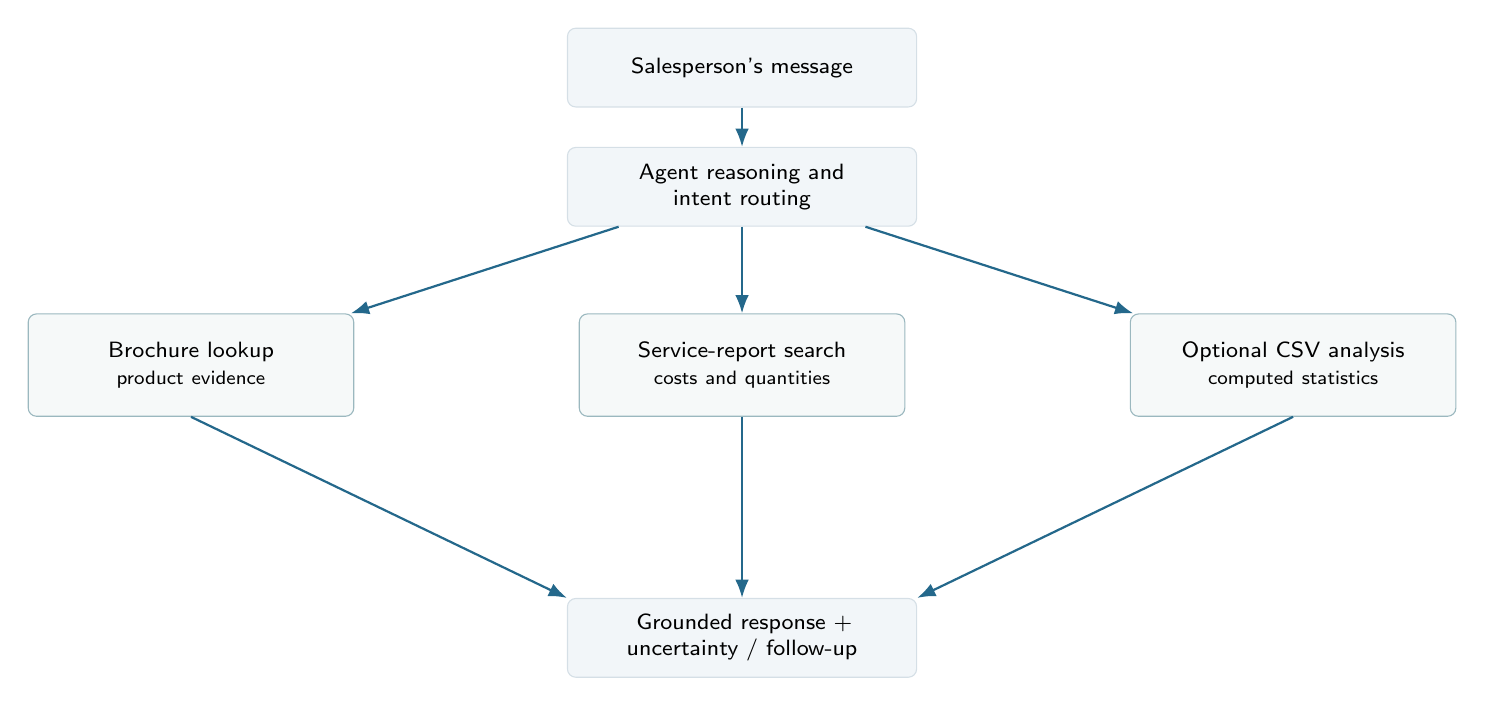
\begin{tikzpicture}[node distance=5mm and 7mm, every node/.style={font=\sffamily\footnotesize,align=center}, block/.style={draw=Rule,fill=Pale,rounded corners=3pt,minimum height=10mm,text width=42mm}, src/.style={draw=Sea!55,fill=Sea!5,rounded corners=3pt,minimum height=13mm,text width=39mm}, arr/.style={-Latex,thick,draw=Blue}]
\node[block] (user) {Salesperson's message};
\node[block,below=of user] (route) {Agent reasoning and\\intent routing};
\node[src,below left=11mm and 27mm of route] (prod) {Brochure lookup\\\scriptsize product evidence};
\node[src,below=11mm of route] (cost) {Service-report search\\\scriptsize costs and quantities};
\node[src,below right=11mm and 27mm of route] (csv) {Optional CSV analysis\\\scriptsize computed statistics};
\node[block,below=23mm of cost] (answer) {Grounded response +\\uncertainty / follow-up};
\draw[arr] (user)--(route);
\draw[arr] (route)--(prod);
\draw[arr] (route)--(cost);
\draw[arr] (route)--(csv);
\draw[arr] (prod.south)--(answer.north west);
\draw[arr] (cost)--(answer);
\draw[arr] (csv.south)--(answer.north east);
\end{tikzpicture}%
}
\end{center}

\textbf{Multiple tools can be appropriate.} The instruction ``which product should we use and what would installing it cost?'' could require a brochure recommendation \emph{and} report-based service assessment. A rigid one-intent-only design may miss this. On the other hand, the assistant should not analyze the entire CSV for a simple pump brochure question.

\textbf{Clarifying questions should be selective.} Ask about a missing detail only when it affects the recommendation or arithmetic enough to matter. For instance, for the Chile repair request, whether Metso supplies the 12 cloths can substantially alter the budget. An overly chatty agent that asks ten questions before answering anything would frustrate a salesperson on a call.

\subsubsection{Correct source-of-truth boundaries}
\begin{tabularx}{\textwidth}{@{}L{39mm}L{45mm}Y@{}}
\toprule\textbf{Question asked} & \textbf{Permitted basis} & \textbf{Avoid}\\\midrule
What does this filter do? & Product brochures & Unsupported remembered specifications or online marketing assumptions.\\
Which product suits unstable filtration? & Brochure features + customer's described need & Guaranteed benefit or model compatibility without proof.\\
What should a technician visit cost? & Historical field-service reports + explicit arithmetic & Arbitrary parts prices, rates, currency conversions or taxes.\\
Are silica and iron readings typical? & Statistical computations on CSV & Generic unsupported claims about standards/targets.\\
Can we guarantee plant performance? & No sufficient basis in this package & Confident guarantee. Explain missing engineering evidence.\\
\bottomrule
\end{tabularx}

\subsubsection{Why uncertainty is a feature, not a weakness}
The supplied materials include imperfect extracted documents, inconsistent terminologies, missing cost lines and heterogeneous service scopes. A defensible assistant must be able to say:
\begin{itemize}
\item ``The brochure supports this capability, but I cannot confirm compatibility with your exact installation.''
\item ``The closest 12-cloth case was in Sweden; the price is a historical comparison, not a Chile quotation.''
\item ``This report mentions an invoice but does not contain the monetary amount.''
\item ``The process values are different from the historical mean; acceptability depends on the customer's specification.''
\end{itemize}
These are not evasions. They are correct responses to missing information and exemplify the primary evaluation criterion of non-invented answers.

\subsection{Data-quality risks and how they change the intended answers}
\begin{longtable}{@{}L{39mm}L{60mm}L{49mm}@{}}
\toprule\textbf{Risk} & \textbf{Observed example} & \textbf{Required caution}\\\midrule\endfirsthead
\toprule\textbf{Risk} & \textbf{Observed example} & \textbf{Required caution}\\\midrule\endhead
Flattened PDF extraction & Brochure tables are represented as plain Markdown text, sometimes without original layout. & Check PDF before asserting delicate numeric specifications.\\
Multiple documents per family & Two distinct Larox PF brochures describe one product family. & Avoid double counting or treating them as separate families.\\
Missing invoice & \code{FSR-0005}, \code{FSR-0028}, \code{FSR-0037} use ``invoice to follow'' / other absent-price wording. & Use as work-description context, not as proof of a price.\\
Truncated record & \code{FSR-0027} ends midway through its cost table. & Label reconstructed figures and cite individual line items.\\
Different scope & \code{FSR-0014} combines cloth replacement and hydraulic service. & Never use bundled total as the pure price of 12 cloths.\\
Currency mismatch & Service records include EUR, CAD, USD, AUD, SEK and ZAR, among others. & Never sum or compare numerically as if units were identical.\\
Tax treatment & \code{FSR-0031} explicitly lists VAT; other documents may not. & Distinguish tax-inclusive and tax-exclusive values.\\
Inconsistent terminology & PF-DS endless-cloth brochure versus multi-cloth replacement counts in reports. & Flag for validation; do not assert identical physical units.\\
Approximate time & Some informal reports contain phrases such as ``about'' or ``roughly''. & Do not present precision absent in the source.\\
Missing engineering units & Flow/level CSV headers provide no explicit engineering unit. & Avoid invented units and operating limits.\\
Time-series gap & One 13-day-7-hour interval is missing between observations. & Do not claim continuous data throughout the date span.\\
Statistical vs contractual normal & A silica value can occur historically without meeting the contract. & Distinguish empirical prevalence from acceptance criteria.\\
\bottomrule
\end{longtable}

\subsection{What a successful answer looks like: acceptance criteria}
This section translates the brief into observable behaviors. It is a requirements checklist, \emph{not} a specification for a large new platform.

\begin{longtable}{@{}L{13mm}L{56mm}L{79mm}@{}}
\toprule\textbf{ID} & \textbf{Requirement} & \textbf{How it can be demonstrated}\\\midrule\endfirsthead
\toprule\textbf{ID} & \textbf{Requirement} & \textbf{How it can be demonstrated}\\\midrule\endhead
R1 & The assistant can converse through a working CLI/simple chat. & Run the program and enter an arbitrary new user message.\\
R2 & It routes requests to the appropriate action. & The product prompt invokes brochure retrieval; the cost prompt invokes service evidence/calculation.\\
R3 & Product responses are brochure-grounded. & Cite at least a file and page; demonstrate that a specification is supported there.\\
R4 & Product recommendations explain fit. & Connect Filter Optimizer features to changing operating conditions.\\
R5 & Service estimates come from the historical reports. & Display the chosen precedents, quantities/rates and arithmetic.\\
R6 & The assistant does not invent unavailable facts. & Ask for a missing site or supply detail; refuse unsupported product pricing or currency conversion.\\
R7 & The model handles imperfect data honestly. & Recognize the truncated FSR and distinguish partial/unknown price evidence.\\
R8 & The runtime source and configuration are reproducible. & README describes dependencies, commands and where local \code{data/} goes.\\
R9 & The public code archive is safe to share. & No \code{data/}, secrets or private API keys in Git history / distributed ZIP.\\
R10 & The recorded demonstration matches the brief. & Run the two exact mandatory prompts live; add the optional prompt only if implemented.\\
R11 & The candidate understands their own code and AI assistance. & Explain routing, evidence choice, calculations, trade-offs and what AI coding tools helped generate.\\
R12 & The final Recright process is completed on time. & Paste code/video links and answer all five recorded questions by the deadline.\\
\bottomrule
\end{longtable}

\subsection{Exactly what must be submitted and when}
\subsubsection{Deliverable 1: publicly accessible code}
The brief allows a public repository (for example GitHub) or a publicly accessible ZIP link (for example OneDrive or Google Drive). The submission must contain the implementation and a short ``how to run'' explanation. It must \emph{not} contain the provided \code{data/} folder or API keys. The receiving evaluator should be able to infer how the authorized local data would be placed for a run.

\subsubsection{Deliverable 2: a 5--7 minute walkthrough video}
Record the screen, describe the key components, and run the following two prompts \emph{live}:
\begin{enumerate}
\item ``We have Larox pressure filters but performance drops whenever our feed grade changes''
\item ``A customer in Chile needs 12 filter cloths replaced on a Larox PF-DS tower press. What should I budget for the service visit?''
\end{enumerate}
If the optional CSV feature is implemented, also run:
\begin{quote}
``The customer is getting 3.1\% silica and 64.5\% iron in their concentrate. They think that's normal. What do you think?''
\end{quote}
If the agent asks a question, answer it briefly and naturally during the recording. Put the video at a publicly accessible URL (for example an unlisted YouTube video) and share the URL.

\subsubsection{Deliverable 3: the separate Recright interview}
A separate invitation from the interview platform supplies the entry link. The candidate pastes \emph{both public links} and records answers to \term{five undisclosed questions about the candidate's own solution}. Each question allows one minute of preparation, up to five minutes of answering and up to three retakes. The session is continuous once started; time should be reserved to complete it in one sitting. The questions are not disclosed ahead of time; any proposed interview questions in prep materials are necessarily speculative.

\subsubsection{Deadline and contacts}
\begin{keybox}
\textbf{Final deadline: Tuesday, 20 October 2026, 23:59 Helsinki local time.} The code link alone is not the full submission: the walkthrough link \emph{and} the Recright interview must also be completed before the deadline.\\[3pt]
\textbf{Assignment questions:} \href{mailto:tarek.ali@metso.com}{tarek.ali@metso.com}.\\
\textbf{Interview-platform technical issues:} \href{mailto:support@recright.com}{support@recright.com}.
\end{keybox}

\subsection{Reasonable priorities under the imposed time box}
The brief is explicitly not a challenge to build the biggest system. A reasonable interpretation of priorities is:\\
\textbf{First:} make product search/recommendations work on the provided brochures, with a traceable citation.\\
\textbf{Second:} make historical-visit cost estimation work, using honest report selection and numerical calculation.\\
\textbf{Third:} test missing-info behavior and both exact evaluation prompts.\\
\textbf{Fourth:} document the setup and prepare the demonstration.\\
\textbf{Fifth (only if time permits):} add basic descriptive flotation analysis, capped at 45 minutes.

A credible account of how one would scale the design to many more documents is useful in the video interview, but the candidate is \emph{not asked to deploy it at scale}. Likewise, AI coding assistance is explicitly acceptable, provided the candidate can explain exactly what the code does.

\subsection{Frequently misunderstood parts of the assignment}
\textbf{Does the candidate have to train an LLM?} No. The brief permits any language, LLM API or agent framework. The requirement is a working agent with candidate-owned implementation, not model pretraining or fine-tuning.

\textbf{Must the candidate use the original PDFs?} No. The provided Markdown extractions may be used as-is, although the PDFs are useful for verifying problematic text extraction and numeric tables.

\textbf{Are the two Larox PF brochure variants two new products?} No. They are two documents about the Larox PF family. The total is 12 brochure pairs, not 24 unrelated products.

\textbf{Can the assistant use online costs or generic ``industry rates''?} No. The historical FSRs are explicitly the sole allowed cost-estimation data source. It can explain that a missing locally supported rate prevents a reliable quotation.

\textbf{Does the Chile prompt require a guaranteed amount in USD?} No. It asks for a rough budget but lacks some crucial commercial details; the data contains a direct Swedish task match and non-identical Chilean rates. A careful estimate or comparable historical range with explicit limitations is preferable to a made-up exact amount.

\textbf{Must the assistant respond without asking anything?} No. The instructions expressly reward asking for missing information when needed. The video walkthrough even explains how to handle clarifying questions on screen.

\textbf{Is the optional flotation test necessary for passing?} No; the brief explicitly says skipping it will not count against the candidate. It is a bonus chance to show disciplined numerical analysis.

\textbf{Is an elaborate GUI an advantage?} No; the evaluators specifically say they are not interested in one. A terminal is enough.

\textbf{Is finishing the code by the deadline sufficient?} No. The public code link, public walkthrough link, and continuous Recright video interview are all required by 23:59 Helsinki time on 20 October.

\subsection{Part I conclusions: what should be understood before coding}
\begin{keybox}
\textbf{The essence of the problem} is task selection plus evidence handling. For a product question, use the brochures; for a cost question, use actual service records and explicit arithmetic; for optional plant-quality assessment, compute with the CSV. A successful agent is small, functioning, grounded, transparent about uncertainty, and understandable to its developer.
\end{keybox}
\begin{enumerate}
\item The main task is a practical industrial sales-support agent rather than a generic question-answering system.
\item It has two required, separate knowledge domains: product capability and field-service cost history.
\item The data package is finite but deliberately heterogeneous: 12 paired brochures, 50 technician reports and one optional hourly process dataset.
\item The most likely first-demo retrieval destination is \code{filter-optimizer.md}, supported by Larox PF context.
\item A central second-demo task analog is \code{FSR-0027.txt}, but it is truncated, from Sweden and not a ready-made Chile quotation.
\item The CSV shows the example's 3.1\% silica and 64.5\% iron values are less favorable than historical center values, but roughly 20.09\% of hourly rows satisfy both threshold conditions.
\item Missing information and data inconsistencies must be disclosed instead of hidden by confident language.
\item Metso will evaluate functioning routing, design decisions, source grounding and the candidate's ability to explain the work; not UI polish or production infrastructure.
\item Delivery is a process: public code, public walkthrough and five-question video interview, all before the deadline.
\end{enumerate}

\subsection{Reference inventory: all 50 field-service files}
The following compact index documents the general task represented by \emph{every} supplied report. It is an orientation aid for navigating the folder, not an assertion that all reported costs are complete or directly comparable. The strongest evidence for each specific new service request must still be evaluated at the source level.
\small
\begin{longtable}{@{}L{22mm}L{72mm}L{55mm}@{}}
\toprule\textbf{File} & \textbf{Equipment / main service described} & \textbf{Location / notable data issue}\\\midrule\endfirsthead
\toprule\textbf{File} & \textbf{Equipment / main service described} & \textbf{Location / notable data issue}\\\midrule\endhead
\code{FSR-0001} & ColumnCell inspection, sparger cleaning and seals. & Chile; detailed USD cost breakdown.\\
\code{FSR-0002} & ColumnCell flotation-column inspection and cleaning. & Sweden; itemized EUR total.\\
\code{FSR-0003} & Orion horizontal slurry pump overheating check / service. & Russia; narrative, bundled total.\\
\code{FSR-0004} & CellStation software and controls servicing. & Peru; narrative, bundled total.\\
\code{FSR-0005} & Concorde Cell maintenance and consumable replacement. & Australia; invoice to follow.\\
\code{FSR-0006} & MD mill-discharge pumps, preventive maintenance and impellers. & Peru; USD total with task summary.\\
\code{FSR-0007} & CellStation commissioning on rougher flotation cells. & Zambia; bundled total.\\
\code{FSR-0008} & Larox PF preventive maintenance and cloth inspection. & Australia; AUD total.\\
\code{FSR-0009} & MD600 mill-discharge pump service. & Canada; detailed cost table.\\
\code{FSR-0010} & Filter Optimizer tuning after feed changes. & Australia; AUD total, no parts.\\
\code{FSR-0011} & Larox PF emergency filtration-line repair. & Canada; CAD bundled total.\\
\code{FSR-0012} & Orion slurry pumps, multi-unit maintenance. & Zambia; detailed cost items.\\
\code{FSR-0013} & Concorde Cell emergency intervention / blocked feed pipe. & Russia; EUR bundled total.\\
\code{FSR-0014} & Larox PF-DS 16-cloth change plus hydraulic/nozzle service. & Canada; fully itemized CAD total.\\
\code{FSR-0015} & Filter Optimizer hardware installation on Larox PF units. & Chile; fully itemized USD total.\\
\code{FSR-0016} & CellStation commissioning and panel/control work. & Australia; abbreviated informal notes.\\
\code{FSR-0017} & Concorde Cell air calibration, rotor-related work. & Sweden; costs refer to agreement.\\
\code{FSR-0018} & Larox PF cloths and equipment checks. & Australia; invoice later / agreement.\\
\code{FSR-0019} & ColumnCell calibration of level and air-related systems. & Canada; structured cost record.\\
\code{FSR-0020} & Concorde Cell equipment and rotor-related inspection. & South Africa; ZAR bundled total.\\
\code{FSR-0021} & MD650 mill-discharge pumps, impellers replaced. & Zambia; invoice to follow.\\
\code{FSR-0022} & ColumnCell, sparger and wash-water nozzle service. & Zambia; invoice to follow.\\
\code{FSR-0023} & Filter Optimizer update and recalibration. & Sweden; structured cost information.\\
\code{FSR-0024} & Concorde Cell rotor/stator wear inspection. & Peru; invoice to follow.\\
\code{FSR-0025} & Two MD650 pumps, impeller replacement and maintenance. & Australia; AUD bundled total.\\
\code{FSR-0026} & Larox PF plate-pack inspection and damaged-plate replacement. & Sweden; SEK itemized costs.\\
\code{FSR-0027} & Larox PF-DS inspection and exactly 12-cloth replacement. & Sweden; closest task match; \textbf{truncated cost table}.\\
\code{FSR-0028} & Larox PF-DS partial cloth change and hydraulic work. & Sweden; unfinished work; price absent.\\
\code{FSR-0029} & MD mill-discharge pump bearings/seal and equipment work. & Sweden; informal notes; contract cost.\\
\code{FSR-0030} & Concorde Cell rotor/stator wear assessment. & Finland; incomplete work; contract cost.\\
\code{FSR-0031} & Larox PF-DS 24-cloth change and hydraulic/nozzle service. & Finland; EUR costs and separate VAT.\\
\code{FSR-0032} & Concorde Cell maintenance and rotor wear inspection. & Sweden; invoice to follow.\\
\code{FSR-0033} & SALA VSP-750 sump-pump maintenance and impeller. & Finland; invoice to follow.\\
\code{FSR-0034} & ColumnCell inspection, cleaning and nozzles. & Chile; itemized USD cost table.\\
\code{FSR-0035} & Filter Optimizer algorithm update and retuning. & Chile; USD bundled total.\\
\code{FSR-0036} & SALA VSP-750 sump-pump service and seals. & Peru; informal notes, variable times.\\
\code{FSR-0037} & Larox PF-DS preventive maintenance and cloth work. & Finland; invoice to follow.\\
\code{FSR-0038} & Orion slurry pump seal and bearing service. & South Africa; informal detailed technician log.\\
\code{FSR-0039} & SALA VSP-750 sump-pump impeller replacement. & Zambia; cost per agreement.\\
\code{FSR-0040} & SALA VSP-750 sump-pump service. & Australia; structured AUD cost record.\\
\code{FSR-0041} & CellStation software update after process changes. & Russia; EUR bundled total.\\
\code{FSR-0042} & Larox PF emergency filter-line repair. & Russia; invoice to follow.\\
\code{FSR-0043} & SALA VSP-750 full inspection and maintenance. & South Africa; ZAR bundled total.\\
\code{FSR-0044} & Larox PF-DS full-cloth/hydraulic maintenance. & Sweden; SEK bundled total.\\
\code{FSR-0045} & Concorde Cell rotor/stator inspection and service. & Zambia; invoice to follow.\\
\code{FSR-0046} & ColumnCell equipment checks and partial servicing. & Chile; contract-based, price not stated.\\
\code{FSR-0047} & SALA VSP-750 column pipe and impeller service. & Canada; CAD bundled total.\\
\code{FSR-0048} & Concorde Cell rotor/stator inspections on two units. & Peru; structured technician report.\\
\code{FSR-0049} & ColumnCell / SonicSparger inspection and cleaning. & Finland; EUR bundled total.\\
\code{FSR-0050} & Orion slurry-pump multi-unit checks and service. & Zambia; informal notes; no quoted final cost.\\
\bottomrule
\end{longtable}
\normalsize

\subsection{Source and reproducibility notes}
\textbf{Direct source of assignment rules:} \code{candidate-brief.md} in the supplied archive and the invitation email dated 12 October 2026. The brief governs priority, scope, source restrictions, public deliverables and timing.

\textbf{Direct source of product statements:} the 12 \code{data/brochures/*.md} files and corresponding original PDFs. Where this report gives a product detail, it identifies the relevant file and (where material) the page range.

\textbf{Direct source of cost comparisons:} relevant \code{data/HistoricalServices/FSR-####.txt} files. All reconstructed arithmetic is clearly differentiated from a source's printed total.

\textbf{Direct source of statistical statements:} the supplied CSV, read as a 4,097-row table; mean, median, quantile, threshold-count, standard-deviation and correlation results were computed from numeric columns. The timestamp analysis used explicit ISO-like year-month-day parsing.

\textbf{Privacy and distribution note:} this document is a candidate's private study report derived from the supplied assignment materials. The official public code submission must exclude the \code{data/} directory. The report itself is not required as part of the public source repository; do not publish supplied material or detailed source extracts under the assumption that the employer's restriction applies only to raw file extensions.

\vfill
\begin{center}
{\sffamily\color{Gray}\footnotesize END OF PART I -- CONTINUED IN PART II}\\[2mm]
{\sffamily\bfseries\color{Navy}AG is your G!}
\end{center}
\clearpage
\section{Part II: My Plan for Solving the Problem}
\sloppy
\label{sec:plan}
\begin{keybox}
\textbf{My engineering objective.} Build a small but rigorously evaluated, evidence-grounded conversational agent that can (1) explain and recommend Metso products exclusively from the supplied brochures, (2) derive transparent preliminary service-visit estimates exclusively from historical field-service reports, and (3) optionally assess flotation readings through deterministic statistical computation. The system must choose the relevant tool or combination of tools from each natural-language message, request only consequential missing facts, and explicitly acknowledge unsupported conclusions. This part is a \emph{prospective implementation plan}; completing this document does not mean the software has been built or tested.
\end{keybox}

\subsection{Planning assumptions, priorities, and scope}
\textbf{Binding employer instructions versus my preferred engineering approach.} Metso's official brief specifies a roughly four-hour implementation time box and, if the optional task is attempted, a maximum of 45 minutes for flotation analysis. My plan below documents the best-quality implementation path, including extra verification and evaluation. These enhancements are \emph{my proposed methods}, not newly imposed employer requirements. I will prioritize a working, explainable solution over unrelated production infrastructure. The final submission must still respect the 20 October 2026, 23:59 Helsinki deadline and the restriction on publishing the \code{data/} folder.

\textbf{Primary optimization objective.} Favor evidence correctness and traceability over the apparent fluency of answers. Specifically: (i) do not hallucinate product specifications; (ii) do not invent cost rates or exchange rates; (iii) separate recorded facts, reconstructed calculations, estimates, and unanswered questions; and (iv) ensure the exact mandatory demonstration prompts and relevant paraphrases work reproducibly.

\begin{tabularx}{\textwidth}{@{}L{31mm}Y L{37mm}@{}}
\toprule\textbf{Priority} & \textbf{Required engineering capability} & \textbf{Proof of completion}\\\midrule
P0 & Executable CLI with autonomously selected brochure lookup and relevant product recommendation. & Live Larox/feed-change prompt; source references.\\
P0 & Executable report retrieval and deterministic, currency-safe service calculation. & Live Chile/12-cloth prompt; evidence ledger and calculations.\\
P0 & Honest clarification, no unsupported claims, repeatable setup and tests. & Negative, missing-data and verification tests.\\
P1 & Reliable semantic and lexical retrieval; structured extraction validation. & Golden query tests and documented failure analysis.\\
P2 & Optional flotation statistics computed from the supplied CSV. & Reproducible third-prompt answer.\\
Out of scope & Fancy UI, fine-tuning, cloud production deployment, multi-agent orchestration for its own sake, live quotes or control-system actuation. & Intentionally not developed.\\
\bottomrule
\end{tabularx}

\subsection{Target architecture and rationale}
\textbf{Design choice: a hybrid agent, not a generic chatbot.} I will use an LLM for natural-language intent interpretation, tool selection, follow-up management, and grounded synthesis, while local Python functions perform document retrieval, numeric operations, and validation. Tool call outputs will be structured, auditable, and typed. The solution remains small enough for a reader to understand end-to-end.

\begin{center}
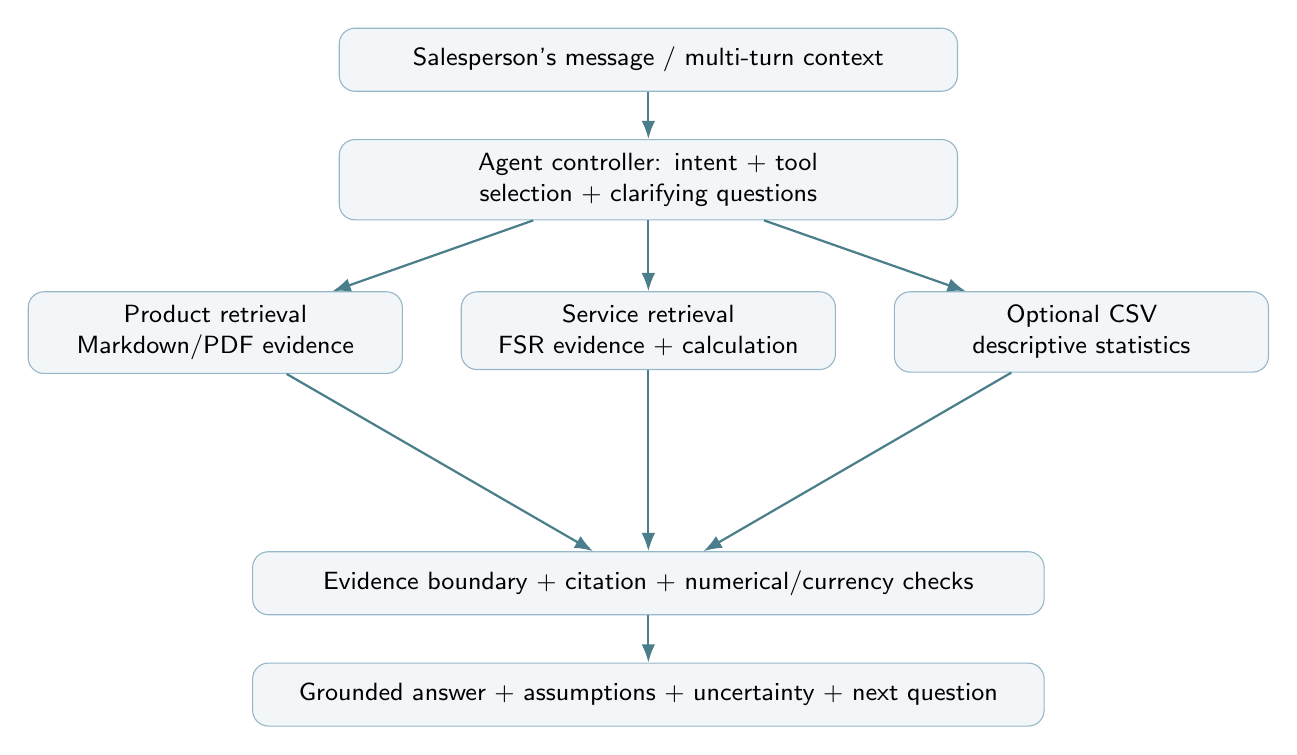
\begin{tikzpicture}[node distance=6mm, >=Latex, every node/.style={font=\sffamily\small}, box/.style={draw=Blue!48,rounded corners=2mm,fill=Pale,align=center,minimum height=8mm,inner sep=5pt},arr/.style={-Latex,thick,draw=Sea}]
\node[box,text width=75mm] (user) {Salesperson's message / multi-turn context};
\node[box,text width=75mm,below=of user] (core) {Agent controller: intent + tool selection + clarifying questions};
\node[box,text width=44mm,below=9mm of core,xshift=-55mm] (bro) {Product retrieval\\Markdown/PDF evidence};
\node[box,text width=44mm,below=9mm of core] (service) {Service retrieval\\FSR evidence + calculation};
\node[box,text width=44mm,below=9mm of core,xshift=55mm] (flot) {Optional CSV\\descriptive statistics};
\node[box,text width=97mm,below=23mm of service] (validation) {Evidence boundary + citation + numerical/currency checks};
\node[box,text width=97mm,below=of validation] (answer) {Grounded answer + assumptions + uncertainty + next question};
\draw[arr] (user) -- (core);
\draw[arr] (core) -- (bro);\draw[arr] (core) -- (service);\draw[arr] (core) -- (flot);
\draw[arr] (bro) -- (validation);\draw[arr] (service) -- (validation);\draw[arr] (flot) -- (validation);
\draw[arr] (validation) -- (answer);
\end{tikzpicture}
\end{center}

\textbf{Recommended stack.} Python 3.12 (or an available recent compatible release); an LLM API that supports structured tool/function calls; \code{pydantic} for schemas; \code{scikit-learn} for baseline TF--IDF; optionally \code{rank-bm25} and local embeddings for hybrid retrieval; \code{pandas} and \code{numpy} for CSV statistics; \code{decimal.Decimal} for monetary arithmetic; \code{pytest} for tests; \code{rich} for readable terminal output; Git for reproducibility. I prefer direct, understandable Python orchestration over a heavy agent framework. SQLite or JSON may hold a small local evidence index; it is not essential to introduce a networked database.

\begin{warnbox}
\textbf{Source-of-truth contract.} Product capabilities and specifications come only from the 12 supplied brochures. Service amounts and rates come only from the 50 supplied reports. Flotation historical claims come from computation on the supplied CSV. Neither general model knowledge nor web search may fill data gaps with unsupported specifications, commercial rates, contractual quality limits, or exchange rates.
\end{warnbox}

\subsection{Implementation phases and dependency order}
\begin{longtable}{@{}L{18mm}L{36mm}L{63mm}L{28mm}@{}}
\toprule\textbf{Stage} & \textbf{Workstream} & \textbf{Concrete deliverable} & \textbf{Requires}\\\midrule\endfirsthead
\toprule\textbf{Stage} & \textbf{Workstream} & \textbf{Concrete deliverable} & \textbf{Requires}\\\midrule\endhead
00 & Environment and safety & Local repo, secure configuration, reproducible run command. & Brief\\
01 & Data audit & Inventory, checksums, risks and corpus coverage. & 00\\
02 & Evidence schema & Typed record models and normalized metadata. & 01\\
03 & Brochure retrieval & Page-grounded search with scored candidate passages. & 02\\
04 & FSR extraction & Structured historical service ledger with quality flags. & 02\\
05 & Cost computation & Strict monetary calculator and comparison selection. & 04\\
06 & Agent controller & Multi-turn tool selection, clarifications and composed output. & 03, 05\\
07 & Evidence guards & Citation verification, claim validation and abstention. & 03--06\\
08 & Flotation (optional) & Deterministic descriptive-analysis tool. & 01, 02\\
09 & Evaluation & Golden tests, integration tests, error taxonomy. & 03--08\\
10 & Developer-friendly CLI & Display sources, tool trace and follow-up responses. & 06--09\\
11 & Distribution & README, tested installation, clean public Git history. & 09--10\\
12 & Demonstration & 5--7 minute walkthrough, public links, Recright answers. & 11\\
\bottomrule
\end{longtable}
\textbf{Milestone gates.} Gate A: data and evidence schemas valid; Gate B: each mandatory tool works by itself; Gate C: the agent autonomously routes both mandatory prompts; Gate D: calculations and citations pass verification; Gate E: public package, recording, and Recright submission are complete.

\subsection{Stage 00 --- Set up the development environment and protect the data}
\textbf{Goal.} Create a local environment that can be rebuilt and cannot accidentally publish assignment files or API credentials.

\textbf{Actions, in order:}
\begin{enumerate}
\item Create a dedicated working directory (e.g., \code{metso-sales-agent/}) with Git initialized, and establish a Python virtual environment.
\item Extract the supplied ZIP \emph{locally} into the expected \code{data/} layout. Retain the original archive as a read-only reference.
\item Add \code{data/}, \code{.env}, \code{.venv/}, caches, generated indexes and logs that may contain source text to \code{.gitignore} before the first commit.
\item Provide \code{.env.example} with placeholder configuration only, such as \code{OPENAI_API_KEY=YOUR_KEY_HERE}; never commit real secrets.
\item Create \code{pyproject.toml} and define a reproducible installation command, development/test commands, and a single CLI entry point.
\item Decide whether an external LLM API is allowed under the employer's handling expectations for restricted source material. The brief allows LLM APIs, but the email marks attachments restricted: avoid unnecessarily persisting raw files in external tools, public prompts, telemetry or logs.
\end{enumerate}
\textbf{Expected artifacts:} project scaffold, \code{.gitignore}, \code{.env.example}, reproducible dependencies, and a short installation section in README.

\textbf{Exit gate:} a fresh local clone can install dependencies, but \code{git status} and \code{git ls-files} do not expose \code{data/} or secrets. A missing API key generates an actionable configuration error instead of a crash.

\subsection{Stage 01 --- Audit and characterize every supplied data source}
\textbf{Goal.} Understand file coverage, format problems, and source limitations \emph{before} choosing parsers or retrieval assumptions.

\subsubsection{01A. Archive and brochure audit}
\begin{enumerate}
\item Verify the package contains one official brief, 12 PDF/Markdown brochure pairs, 50 numbered FSR text files, and one CSV. Flag missing or duplicate stems.
\item Preserve document stems and page boundaries such as \code{## Page 2}; map each PDF to its Markdown counterpart.
\item Log brochure title/product family, number of extracted pages, page-marker positions, table/layout risk, and any mismatches in technical specifications.
\item Manually inspect high-risk numeric claims in the original PDFs, especially Larox PF model specifications and the PF-DS cloth description.
\item Treat the two Larox PF brochures as two sources describing a related product family; do not count their overlapping claims as independent proof of multiple models.
\end{enumerate}
\subsubsection{01B. Field-service audit}
\begin{enumerate}
\item Enumerate \code{FSR-0001.txt} to \code{FSR-0050.txt}; classify each as itemized, narrative total, or cost-unavailable/partial.
\item Record the country, site, date, equipment, activities, quantities, parts, labor hours, travel hours, currency, rate, tax, and total \emph{when explicitly present}.
\item Tag missing invoices, approximate hours, truncated reports, conflicting subtotals, ambiguous part units, contract-only pricing, and blended service scopes.
\item Verify FSR-0027 (matching 12-cloth work but truncated), FSR-0014 and FSR-0031 (different quantities/scopes), and Chile reports FSR-0001, 0015, 0034, 0035, 0046.
\item Check for conflicting hour descriptions and distinguish reported/billed hours from a recomputed activity timeline. Do not silently overwrite either.
\end{enumerate}
\subsubsection{01C. Flotation file audit}
\begin{enumerate}
\item Parse timestamps and numeric columns, inspect nulls/duplicates/time gaps, and list 24 fields by engineering meaning.
\item Preserve original numeric precision; do not infer missing units for reagent flows, air flows or column levels.
\item Establish baseline descriptive statistics and guard against treating time-correlated hourly measurements as independent operating experiments.
\end{enumerate}
\textbf{Artifacts:} \code{docs/data_audit.md} (\emph{private} if detailed source extracts are included), an inventory table, and a data-quality issue log. The code repository can share the methodology but must not publish the employer's source records.

\textbf{Exit gate:} all 76 actual files have an accounted-for purpose; the listed critical anomalies are recorded; no unsupported normalization has destroyed original values.

\subsection{Stage 02 --- Define canonical evidence schemas and traceability}
\textbf{Goal.} Give each downstream tool consistent typed inputs and outputs, with strong provenance.

\textbf{Product evidence record.} \code{document_id}, \code{product_family}, \code{page_number}, \code{chunk_id}, \code{source_path}, \code{source_excerpt}, \code{extraction_method}, and \code{quality_flags}. Keep enough original text to check whether the final claim is actually supported, without exposing the full data in the public repository.

\textbf{Service evidence record.} Group the fields as follows:
\begin{itemize}
\item Identity: \code{report_id}, \code{site}, \code{country}, and \code{date}.
\item Scope: \code{equipment_model}, \code{job_actions}, \code{quantity}.
\item Timing and charges: \code{labor_hours}, \code{travel_hours}, \code{cost_items}, \code{currency}, \code{tax_treatment}, and \code{reported_total}.
\item Traceability: \code{cost_status}, \code{source_span}, \code{quality_flags}.
\end{itemize}
Optional or missing numeric fields remain null, never fabricated zero.

\textbf{Cost item record.} A structured tuple of \emph{type, quantity, unit, rate, currency, extended cost, tax flag, evidence reference, quality status}. Store \emph{observed value} separately from \emph{derived value} to make arithmetic review possible.

\textbf{Response contracts.} Tools return a route/intent, supporting evidence IDs, numbers with units, calculation steps and unknowns. The status is one of \code{SUPPORTED}, \code{PARTIAL}, \code{INSUFFICIENT}, or \code{CONFLICTING}. The LLM may phrase a response but cannot upgrade partial evidence into a verified fact.

\begin{examplebox}
\textbf{Example service-item contract (illustrative only).} ``Report FSR-0027 / item filter cloth / quantity 12 / unit cost 98 EUR / line amount 1176 EUR / observed; on-site hours 8.4 h / labor rate 78 EUR per hour / derived amount 655.20 EUR / quality: report truncated.'' The record is \emph{an evidence statement}, not a validated offer for the Chilean customer.
\end{examplebox}

\textbf{Exit gate:} parser outputs are validated before use; unknown currency, missing parts prices and invalid quantities cannot be silently accepted as complete prices. Every output points back to a source file and, where available, page/section or text span.

\subsection{Stage 03 --- Implement brochure-grounded product retrieval}
\textbf{Goal.} Find the relevant \emph{solution to a customer problem}, not merely the document containing the most repeated product name.

\textbf{03A. Ingestion and indexing.} Read all 12 Markdown brochures with UTF-8; split at explicit page markers; optionally split lengthy pages into coherent passages (initial target roughly 350--650 tokens with overlap, adjusted for natural headings). Keep page number, document stem, local offsets, and product-family metadata. Never flatten away citation identity. Verify numeric specification tables against source PDFs when needed.

\textbf{03B. Lexical baseline.} Implement TF--IDF or BM25 ranking for exact model names, technical terms, and part references. Normalize common casing/hyphen differences without merging PF with PF-DS. Use a concise domain synonym dictionary for user wording versus brochure wording, but do not write hidden answers to the demonstration prompts.

\textbf{03C. Optional semantic retrieval.} Evaluate embeddings on a labeled set of paraphrased product questions. If semantic retrieval beats the lexical baseline, combine scores or ranks (e.g., reciprocal rank fusion) and, if warranted, rerank the top candidates. It is not necessary to operate a vector database for this small corpus.

\textbf{03D. Evidence selection.} Return a bounded set of passages with \code{source}, \code{page}, \code{score}, and \code{excerpt}. Ask the LLM to connect the customer problem to a documented mechanism and to distinguish a \emph{promising investigation} from guaranteed equipment compatibility.

\begin{keybox}
\textbf{Golden product example.} For ``We have Larox pressure filters but performance drops whenever our feed grade changes'', the system should find \code{filter-optimizer.md}, particularly pages 2--3, and may use Larox PF brochures for context. It should say that changing feed grade alone does \emph{not} prove changes in slurry density, moisture, or particle size. The agent should ask whether throughput, cycle time, or cake moisture is deteriorating and should not promise compatibility with an unspecified installation.
\end{keybox}

\textbf{Quality tests.} Query the corpus with exact names, paraphrases, ambiguous failure descriptions, false premises, conflicting specs, and unknown products. Measure whether the expected evidence appears in the top-ranked results and whether the agent refuses unlisted performance guarantees.

\textbf{Exit gate:} the mandatory product demo and materially different paraphrases retrieve the correct underlying brochure, with source- and page-specific grounded answers.

\subsection{Stage 04 --- Extract and verify the historical service reports}
\textbf{Goal.} Convert semi-structured technician prose into an auditable \emph{historical evidence ledger}, while preserving original text and incompleteness.

\textbf{04A. Parse context.} For each report, detect report ID, equipment type and model, country and customer site, date, technician observations, exact work completed, parts quantities, and whether the visit was completed. A report's title or short summary alone is insufficient to distinguish inspection from actual replacement work.

\textbf{04B. Parse time and money.} Extract separately: (a) reported on-site hours; (b) time window or activity timeline; (c) travel hours; (d) charged labor and travel rates; (e) unit price, quantity, subtotal and currency for each part; (f) tax or other fees. Classify whether each value was explicit, reconstructed by arithmetic, approximate, or absent. Validate all amounts with \code{Decimal}.

\textbf{04C. Track uncertain reports.} Do not assign numeric cost to ``invoice to follow'', ``cost as per agreement'', or an unpriced visit. Store such visits as task/effort evidence only. For bundled totals, mark that the scope cannot safely be decomposed into a per-cloth price. For truncated cost tables, mark incomplete and use clearly labeled arithmetic reconstruction only when individual rates/quantities are independently known.

\textbf{04D. Human-reviewed reference cases.} Create a small, private ``gold'' extraction sheet for representative reports; compare the parser against it and manually review mismatches. At minimum include FSR-0027, FSR-0014, FSR-0031, one Chile USD report, and one unpriced narrative report.

\begin{warnbox}
\textbf{Critical FSR-0027 consistency tests.} The source provides a reported \(8.4\) on-site hours and a listed activity window of 07:30--16:15 (\(8.75\) elapsed hours). The associated working total using \(8.4\) hours is a reconstructed EUR 2,215.40, while substituting \(8.75\) hours would change the arithmetic to EUR 2,242.70. These are competing \emph{calculation assumptions}, not two validated invoices. The cost table itself is also truncated. Retain both time measurements and never assert that the alternative duration is billable without additional evidence.
\end{warnbox}

\textbf{Exit gate:} each report has a traceable record and quality status; the parser distinguishes completed and incomplete work and never treats an unpriced report as a free-of-charge service. A small human-reviewed set matches the original text for all material fields.

\subsection{Stage 05 --- Build an evidence-based service-cost estimator}
\textbf{Goal.} Return a commercially useful, transparent \emph{preliminary planning comparison} without disguising differences in currency, geography, scope or report quality.

\subsubsection{05A. Interpret the customer request}
Represent the incoming request as \emph{country/site, equipment model, task type, quantity, requested currency, parts supplied by whom, and requested inclusion of travel/tax}. For the mandatory prompt, the observed values are \emph{Chile, Larox PF-DS, 12 filter cloths}; precise site, travel origin, parts supply, crew and tax remain unknown. Avoid asking about details that do not materially affect the useful answer.

\subsubsection{05B. Retrieve precedents on two axes}
\textbf{Task similarity:} prefer the same equipment, action, quantity and finished work. \code{FSR-0027} is the strongest 12-cloth PF-DS activity analog; \code{FSR-0014} and \code{FSR-0031} have related but broader scopes. \textbf{Geographic context:} retrieve Chilean visits such as \code{FSR-0001}, \code{FSR-0015}, and \code{FSR-0034} to understand \emph{historically recorded} labor/travel charges, not to imply current tariff validity or identical scope. Do not use the cost of installing Filter Optimizer controllers as a cloth-replacement price.

\subsubsection{05C. Separate evidence from arithmetic}
For each item \(i\), let \(q_i\) be a verified quantity and \(r_i\) a verified monetary rate in the \emph{same currency}. The only allowed cost arithmetic is:
\begin{equation}
C_{\mathrm{known}} = C_{\mathrm{labor}}+C_{\mathrm{travel}}+\sum_i q_i r_i + C_{\mathrm{other\ known}}.
\end{equation}
When amounts are in incompatible currencies, \emph{do not sum them}. Missing charges stay unknown and should be listed explicitly, rather than replaced by zero. Historical amounts may be shown individually as examples, not transformed into a quote without evidence.

\subsubsection{05D. Define estimate status and safe output}
Use the distinct statuses \code{HISTORICAL_ANALOG}, \code{PARTIAL_ESTIMATE}, and \code{SUFFICIENT_FOR_ROUGH_BUDGET} (the last only when a defensible common-currency calculation exists and scope is clear). Include a breakdown of observed/derived items, report IDs, dates, geography, exclusions, inconsistency flags, and one concise follow-up question if needed.

\begin{examplebox}
\textbf{Desired response shape for Chile.} ``A directly comparable 12-cloth PF-DS intervention appears in FSR-0027 (Sweden, 2023). Using that report's item rates and its stated 8.4 billed/on-site hours gives a reconstructed EUR 2,215.40 historical component total. Its cost table is truncated and its activity timeline differs from the stated hours. This is \emph{not} a Chile-specific price. Chilean reports record USD labor/travel rates for other equipment and scopes, so I cannot responsibly combine them with EUR parts into one supported total. Is the customer supplying the cloths, and at which Chilean site will the work occur?'' The final implementation must compute these values, not paste a hard-coded answer.
\end{examplebox}

\textbf{Special handling rules:}
\begin{itemize}
\item Do not silently infer a fixed crew size, accommodation, tax rate or technician origin.
\item Distinguish part \emph{quantity} from physical unit: the PF-DS brochure describes an endless-cloth arrangement while some reports count multiple ``cloths.'' Flag this ambiguity before using the estimate commercially.
\item Do not compute cross-currency averages; if comparing multiple records, group and label the results by currency and scope.
\item Do not extrapolate complete job totals linearly with cloth count when fixed travel/hydraulic tasks are bundled.
\item Label historical rates with the year and site; they are not guaranteed present-day market tariffs.
\end{itemize}
\textbf{Exit gate:} unit tests reproduce the verified FSR arithmetic exactly, detect missing prices and mismatched currencies, and make the required Chile prompt return an appropriately qualified, evidence-backed answer.

\subsection{Stage 06 --- Build the autonomous conversational agent controller}
\textbf{Goal.} Connect the tools so the user provides \emph{only a natural-language message}; the agent itself chooses the appropriate action.

\textbf{06A. Register a small tool set.} Each tool returns typed data; the user never manually selects a mode.
\begin{itemize}
\item \code{search_product_brochures(query)} --- page-grounded product evidence.
\item \code{search_service_reports(...)} --- similar jobs and local-rate evidence.
\item \code{calculate_service_estimate(...)} --- validated components and arithmetic.
\item \code{analyze_flotation(...)} --- optional computed process comparison.
\end{itemize}

\textbf{06B. Define agent execution loop.}
\begin{enumerate}
\item Receive a message and available conversation history.
\item Choose zero, one, or several allowed tools based on intent and missing fields.
\item Validate arguments before executing each tool; reject unsupported names or malformed types.
\item Run retrieval/calculation tools and return their structured results to the controller.
\item If more evidence is necessary, permit a bounded additional tool call; otherwise synthesize the answer with citations, explicit assumptions and relevant next question.
\item Store only the minimum context needed for a follow-up (e.g., model, site, parts-supply assumption) in the conversation state.
\end{enumerate}
\textbf{06C. Combined questions.} Support user messages such as ``Which product addresses feed variability, and what do similar installation visits cost?'' by invoking both brochure and service tools when applicable. The former can suggest a relevant feature; the latter must refuse to imply the same product necessarily has the requested historical installation cost when there is no matching record.

\textbf{06D. Operational robustness.} Establish maximum tool-call rounds, timeouts, API failure messages, deterministic validation of tool arguments, and preservation of question context across one or two clarifying turns. Any routing fallback must not mislabel unsupported answers as sourced facts.

\textbf{Exit gate:} the two exact mandatory prompts automatically select the correct tools; paraphrases and combined questions work; one natural follow-up updates the context without restarting the conversation.

\subsection{Stage 07 --- Validate claims, source boundaries, and uncertainty}
\textbf{Goal.} Prevent the answer-generation step from negating the safeguards provided by the tools.

\begin{longtable}{@{}L{35mm}L{78mm}L{32mm}@{}}
\toprule\textbf{Control} & \textbf{Implementation rule} & \textbf{Pass criterion}\\\midrule\endfirsthead
\toprule\textbf{Control} & \textbf{Implementation rule} & \textbf{Pass criterion}\\\midrule\endhead
Citation existence & Every returned brochure citation refers to a real stem/page and a retrieved passage. & No invented page or report IDs.\\
Citation support & For sensitive claims, test that the passage meaning supports the claim; human-review a sample. & No unsupported numeric specifications.\\
Currency integrity & Every monetary arithmetic result carries one currency; reject mixed-currency addition. & Invalid additions blocked.\\
Cost provenance & Each subtotal points to observed line items and the derived arithmetic. & Recomputable result.\\
Source isolation & Product facts from brochures; rates only from FSRs; statistics only from CSV. & No source-domain crossover.\\
Missing evidence & If insufficient, answer partially, ask once, or abstain clearly. & No fabricated figures.\\
Data quality & Report truncated, bundled, approximate and contradictory values. & Warnings included.\\
Prompt-injection defense & Treat retrieved document text as untrusted content, not model instructions. & Ignore hostile ``instructions'' in documents.\\
API error handling & If a tool/model call fails, report failure without presenting it as a factual negative result. & Clear recoverable errors.\\
\bottomrule
\end{longtable}

\textbf{Important design distinction.} A valid citation \emph{location} does not automatically prove a claim. Citation validity checks whether the file/page exists; citation support tests whether the retrieved excerpt actually entails the claim. Both matter. Likewise, an estimate with arithmetic precision can still be \emph{commercially uncertain} if its service scope is mismatched.

\textbf{Exit gate:} invalid citations, invented prices, missing-data fabrications, hidden currency conversions, and unsupported compatibility guarantees are rejected in targeted tests.

\subsection{Stage 08 --- Implement optional flotation data analysis}
\textbf{Goal.} Use the 4,097 hourly records to answer the provided silica/iron scenario using actual numbers, not inferred industry specifications.

\textbf{08A. Data handling.} Load the CSV once, preserve timestamps and numeric columns, verify missingness and the known time gap, and never invent units not present in the headers. Avoid claiming it represents a continuous full-period dataset.

\textbf{08B. Numerical functions.} Compute historical means, medians, quantiles, sample sizes, the empirical frequency of threshold conditions, and where appropriate a descriptive correlation. Return a typed result including assumptions about the comparison direction and the denominator \(N\).

For the required example, the calculations to reproduce are:
\begin{align}
P(S\ge 3.1\%) &= 981/4097 \approx 23.94\%,\\
P(F\le 64.5\%) &= 1142/4097 \approx 27.87\%,\\
P(S\ge 3.1\%, F\le 64.5\%) &= 823/4097 \approx 20.09\%.
\end{align}
Here \(S\) denotes silica percentage and \(F\) iron percentage in the concentrate. These are \emph{sample proportions of historical records}, not estimates of a contractual reject rate.

\textbf{08C. Interpretation.} State that 3.1\% silica exceeds the historical mean (about 2.327\%), while 64.5\% iron is below its historical mean (about 65.050\%). The joint condition is present in about one-fifth of recorded hours: not unprecedented, yet not automatically acceptable. Do not identify a causal mechanism or prescribe process settings solely from these associations.

\textbf{08D. Relevant follow-up.} Ask about the customer's contractual quality limits, recent operating trends, or feed changes. If suggesting an area for investigation (such as pulp level or air-flow control), consult an appropriate brochure to describe the capability \emph{without} promising an improvement in measured quality.

\textbf{Exit gate:} the numbers match direct Pandas calculations; edge cases with missing or invalid parameters fail clearly; the answer distinguishes historical occurrence from acceptable concentrate specification.

\subsection{Stage 09 --- Create a genuine evaluation and regression-test suite}
\textbf{Goal.} Establish evidence that the agent works beyond two memorized demonstration strings.

\textbf{09A. Golden test set.} Prepare a small \emph{private} labeled set of 30--50 questions, spanning product selection, exact specifications, costs, mixed questions, unknown products, currency conflicts, ambiguous sites, follow-up replies, and optional flotation queries. For each test, label expected route(s), key evidence IDs and unacceptable claims. Do not seed answers into runtime code.

\textbf{09B. Test layers.}
\begin{itemize}
\item \textbf{Unit tests:} page parsing, service extraction, currency checks, Decimal arithmetic, CSV statistics, and missing-field validation.
\item \textbf{Retrieval tests:} exact names and semantically varied requests, with source-level relevance judgments and retrieval recall at rank \(k\).
\item \textbf{Agent integration tests:} tool selection, multi-tool execution, one-step clarification, refusal when evidence is absent, and recovery from invalid arguments.
\item \textbf{Adversarial tests:} invented price requests, forged citations, requests to ignore source restrictions, hostile pseudo-instructions in retrieved text, and incorrect units.
\item \textbf{Demo regression tests:} both exact mandatory prompts, and the exact optional prompt if built; run all immediately before recording.
\end{itemize}

\textbf{09C. Suggested quality indicators (targets, not achieved results).}\par\medskip\noindent
\begin{tabularx}{\textwidth}{@{}L{39mm}L{38mm}Y@{}}
\toprule\textbf{Metric} & \textbf{Suggested target} & \textbf{Measurement method}\\\midrule
Intent routing & \(\geq95\%\) labeled accuracy & Correct tool route on hand-labeled holdout prompts.\\
Relevant evidence & \(\geq95\%\) recall@5 & Expected source passage among five retrieved results.\\
Cost arithmetic & 100\% on fixtures & Exact Decimal comparisons for explicit line items.\\
Currency safety & Zero cross-currency sums & Rejection tests with EUR/CAD/USD inputs.\\
Citation integrity & All references exist & Verify file IDs, pages and passage IDs.\\
Missing-data conduct & No fabricated prices & Unknown-rate and unpriced-report tests.\\
Reproducibility & Fresh setup succeeds & Recreate environment and execute smoke tests.\\
\bottomrule
\end{tabularx}\par\medskip
The targets are aspirational acceptance criteria selected for this implementation; neither the brief nor the current analysis demonstrates that these scores have been achieved. Report failures alongside successes rather than hide them.

\textbf{09D. Error analysis.} Record whether a failure originated in routing, retrieval, report extraction, arithmetic, synthesis or unsupported inference. Fix root causes in the correct component and rerun the same test set. Keep benchmark prompts separate from source-code special cases.

\textbf{Exit gate:} all arithmetic/security unit tests pass; the exact demo prompts work; documented retrieval and routing evaluation meets a consciously chosen threshold or describes observed weaknesses explicitly.

\subsection{Stage 10 --- Build a clear, minimal command-line demonstration}
\textbf{Goal.} Make the technical workflow inspectable without spending effort on an unnecessary graphical interface.

\textbf{CLI behavior.} Launch with a single documented command; prompt for user text; show a concise action trace such as \code{Route: Product lookup -> Source: filter-optimizer.md p. 2--3}; render the final answer and relevant warnings; keep interaction state for a clarifying reply; handle \code{exit} and API failures politely. A \code{--verbose} flag can show tool arguments/evidence IDs for the walkthrough while ordinary use stays compact.

\textbf{Trace transparency.} Do \emph{not} expose private model reasoning or dump entire confidential reports. Display factual evidence IDs, selected tool names, and numeric calculation steps instead. If a follow-up is asked, the salesperson can type a brief response in the same terminal session.

\textbf{Exit gate:} a reviewer can understand how the agent selected the action and arrived at the result, and the walkthrough runs without manual editing between prompts.

\subsection{Stage 11 --- Package, document, and safely publish the code}
\textbf{Goal.} Deliver a self-explanatory, reproducible \emph{public code-only} artifact.

\textbf{Proposed project tree (illustrative; module count may be reduced):}
\begin{Verbatim}[fontsize=\footnotesize]
metso-sales-agent/
  main.py
  pyproject.toml
  README.md
  .env.example
  .gitignore
  src/metso_agent/
    agent.py                # tool routing and context
    schemas.py              # typed input/output records
    ingestion/              # brochure and FSR parsers
    retrieval/              # lexical/semantic search
    tools/                  # product, service, flotation
    validation/             # provenance/currency checks
    cli.py
  tests/                    # unit and integrated behavior
  data/                     # LOCAL ONLY -- never publish
\end{Verbatim}

\textbf{README requirements.} Explain the business objective, architecture and why each tool exists; Python requirements, local setup, environment variables, authorized \code{data/} placement, run command, three demonstrations, testing command, trust boundaries, known limitations, and a future scaling strategy. Include neither credentials nor embedded employer data.

\textbf{Suggested local commands (Windows PowerShell):}
\begin{Verbatim}[fontsize=\footnotesize]
py -3.12 -m venv .venv
.\.venv\Scripts\Activate.ps1
python -m pip install --upgrade pip
python -m pip install -e ".[dev]"
python main.py
pytest -q
\end{Verbatim}
Adjust the installation command to the final packaging configuration; verify it on a clean environment before publishing. For API-driven runs, place a valid key in a local, ignored \code{.env} rather than hard-coding it.

\textbf{Publishing gate.} Inspect \code{git status}, \code{git ls-files} and the repository \emph{history} for data or secrets. Scan README/tests for copied confidential source excerpts and real customer details. Verify the public link in a private/incognito browser and confirm code is readable without special access. A \code{.gitignore} created \emph{after} committing sensitive files does not remove them from history.

\textbf{Exit gate:} another developer can read the README, install the package and run it with their own authorized local copy of the source data; the public repository contains neither the data folder nor private credentials.

\subsection{Stage 12 --- Record the walkthrough and complete the interview}
\textbf{Goal.} Demonstrate real, understandable behavior with the two mandated requests and submit all artifacts before the deadline.

\textbf{Walkthrough target: six minutes within the required 5--7 minute window.}\par\medskip\noindent
\begin{tabularx}{\textwidth}{@{}L{26mm}Y@{}}
\toprule\textbf{Time} & \textbf{What the viewer should see}\\\midrule
00:00--00:40 & Problem summary, objectives and evidence-only source boundaries.\\
00:40--01:35 & Agent controller, retrieval, calculator and validation components.\\
01:35--02:55 & Exact Larox pressure-filter changing-feed prompt; document/page citations and one meaningful follow-up if needed.\\
02:55--04:40 & Exact Chile, PF-DS, 12-cloth prompt; report selection, EUR historical analog, local USD evidence and clear limitations.\\
04:40--05:30 & Optional silica/iron prompt, only if the feature has been implemented and tested.\\
05:30--06:20 & What was validated, limitations, how AI coding assistance was used, and scaling rationale.\\
\bottomrule
\end{tabularx}\par\medskip

\textbf{Mandatory product prompt.} ``We have Larox pressure filters but performance drops whenever our feed grade changes''.

\textbf{Mandatory cost prompt.} ``A customer in Chile needs 12 filter cloths replaced on a Larox PF-DS tower press. What should I budget for the service visit?''

\textbf{Optional prompt.} ``The customer is getting 3.1\% silica and 64.5\% iron in their concentrate. They think that's normal. What do you think?''

\textbf{Before recording.} Test the actual API configuration, terminal readability, audio, recording permission, and both live prompts. If the agent asks a question, give one short realistic answer on screen. Do not paste precomputed canned answers and misrepresent them as live agent behavior.

\textbf{Submission.} Upload the 5--7 minute video to an accessible link (unlisted video is acceptable), verify that it opens without permission requests, and provide the code and video URLs in the separate Recright session. Finish all five unseen interview questions in one sitting: each permits one minute of preparation, up to five minutes of answering and up to three retakes. The full submission, \emph{not only the GitHub repository}, is due 20 October 2026 at 23:59 Helsinki time.

\textbf{Exit gate:} both URLs work for viewers outside the account, and the full Recright process is completed before the deadline.

\subsection{System-wide acceptance checklist}
\begin{longtable}{@{}L{13mm}L{111mm}L{24mm}@{}}
\toprule\textbf{ID} & \textbf{Observable acceptance requirement} & \textbf{Owner / proof}\\\midrule\endfirsthead
\toprule\textbf{ID} & \textbf{Observable acceptance requirement} & \textbf{Owner / proof}\\\midrule\endhead
A01 & User can enter free-text requests with no manual mode selection. & CLI test\\
A02 & Product questions use brochure evidence with actual file/page references. & RAG test\\
A03 & Product recommendation connects documented features to the user's stated need. & Golden prompts\\
A04 & Cost questions search analogous FSR tasks and local-country examples separately. & Retrieval test\\
A05 & Cost calculations are reproducible and use \code{Decimal}. & Unit test\\
A06 & Missing rate, inconsistent hours and truncated FSR data are surfaced. & Adversarial test\\
A07 & No conversion or addition across currencies without an authorized rate. & Currency test\\
A08 & Multi-turn follow-up retains the correct equipment and task context. & Session test\\
A09 & Combined product and service question can invoke multiple tools. & Integration test\\
A10 & No invented product spec, price, guaranteed compatibility or contractual limit. & Negative tests\\
A11 & Optional flotation result uses calculated historical sample proportions. & CSV fixture\\
A12 & Source and credential files never enter the public code repository. & Git audit\\
A13 & README setup works in a clean environment with authorized local data. & Install smoke\\
A14 & Walkthrough plays and contains exact demonstration prompts. & Video review\\
A15 & Code/video links and all five Recright answers submitted before cutoff. & Submission check\\
\bottomrule
\end{longtable}

\subsection{Risk register and fallback strategies}
\begin{longtable}{@{}L{34mm}L{65mm}L{48mm}@{}}
\toprule\textbf{Risk} & \textbf{Impact} & \textbf{Mitigation / fallback}\\\midrule\endfirsthead
\toprule\textbf{Risk} & \textbf{Impact} & \textbf{Mitigation / fallback}\\\midrule\endhead
Semantic retrieval misses Filter Optimizer & First demo answers from a generic PF brochure. & Maintain a lexical baseline, synonym checks, and evaluated hybrid retrieval.\\
LLM invents a service quote & Financially misleading answer. & Arithmetic and cost provenance only in deterministic tools; explicit abstention.\\
Irregular FSR parsing & Wrong hours, rates or part quantity. & Source spans, quality flags, human-reviewed gold cases.\\
Incomplete or conflicting invoices & Unsupported precise totals. & Label analog vs estimate; show conflicting data and ask a clarification.\\
Currency and tax mismatch & Incorrect monetary summation. & Currency-typed values, tax flag, fail-closed validation.\\
LLM API connection fails & Agent demo cannot run. & Preflight API test, clear error/retry; retain local deterministic unit tests.\\
Too much abstraction & Hard to explain within seven minutes. & Favor direct Python modules and a single small controller.\\
Confidential data leak & Violates submission restriction. & Ignore data/ and caches; audit Git history and upload contents.\\
Deadline compression & Code succeeds but Recright unfinished. & Freeze working build early; reserve a separate demo/interview window.\\
\bottomrule
\end{longtable}

\subsection{How I would explain scalability without overbuilding}
The provided task contains only 12 brochures and 50 service reports. I should \emph{not} deploy a complex cloud stack for it. Yet modular boundaries create a credible path to larger corpora: switch local document indexing to a managed/full-text and vector-retrieval service; batch-ingest new reports with provenance, version IDs and validation; retain typed cost records in a governed database; introduce document-level access controls and observability; evaluate retrieval drift and incomplete-record rates; and separate background indexing from interactive queries. These are \emph{future extension options}, not capabilities claimed for the take-home deliverable.

\subsection{My implementation sequence and decision gates}
\begin{enumerate}
\item \textbf{Establish one reproducible run command} and ensure the \code{data/} directory is ignored. \emph{Do not proceed until the repository is safe.}
\item \textbf{Inventory and audit the actual source material}; write down anomalies rather than assuming clean invoices.
\item \textbf{Make the typed evidence ledger}; keep observed and calculated fields separate.
\item \textbf{Finish and test brochure retrieval as an independent Python function}; verify the correct page appears for the required Larox question.
\item \textbf{Finish and test FSR search plus Decimal calculation}; verify the FSR-0027 analog and the Chile data limitations.
\item \textbf{Add the agent controller}; ensure it chooses tools from free-text input, supports clarification and preserves conversation context.
\item \textbf{Add evidence/currency validation and negative tests}; do not allow unsupported assertions through response formatting.
\item \textbf{Build the optional CSV analyzer only after the mandatory flows pass}; calculate from the file at runtime.
\item \textbf{Run all evaluation cases, fix regressions, and freeze dependencies}; prioritize correctness over new features.
\item \textbf{Publish code only, record live walkthrough, verify both links, and complete Recright.}
\end{enumerate}

\begin{keybox}
\textbf{Definition of done.} The project is done \emph{only} when the public source code is safe and reproducible, the agent successfully routes and answers both exact mandatory prompts with authentic evidence, monetary arithmetic is traceable and currency-safe, unsupported claims are handled honestly, the walkthrough is viewable, and all five Recright answers have been submitted before the employer's deadline.
\end{keybox}


\subsection{Execution work tickets: exact artifacts and completion tests}
The following is my day-to-day checklist. Each ticket names the file or evidence to create and a test that can be run before proceeding. These are \emph{planned artifacts}, not files that already exist in the submitted code.
\begin{longtable}{@{}L{14mm}L{48mm}L{82mm}@{}}
\toprule\textbf{Step} & \textbf{Files / outputs to create} & \textbf{Definition of done --- tangible evidence}\\\midrule\endfirsthead
\toprule\textbf{Step} & \textbf{Files / outputs to create} & \textbf{Definition of done --- tangible evidence}\\\midrule\endhead
00 & \code{pyproject.toml}, \code{.gitignore}, \code{.env.example}, \code{README.md} skeleton & \code{python --version} reports a supported release; test runner starts; Git tracks no \code{data/}, credentials or private logs.\\
01 & \code{docs/data_audit.md} (private); inventory script & Exactly 12 MD and 12 PDF brochures, 50 distinct FSRs, CSV with 4,097 rows/24 columns; anomaly log exists.\\
02 & \code{schemas.py}, canonical evidence fixtures & Invalid currencies/negative quantities or missing required source identifiers are rejected or explicitly marked missing.\\
03 & \code{brochure_loader.py}, \code{product_search.py} & For the mandatory Larox question, retrieval returns a relevant Filter Optimizer passage with document ID/page; paraphrases also tested.\\
04 & \code{service_parser.py}, local \code{service_ledger.json} & Source trace for FSR-0027 and Chile reports; truncation, ambiguous labor hours, and absent invoices have named flags.\\
05 & \code{cost_estimator.py}, \code{test_costs.py} & EUR 2,215.40 is reproduced as the historical FSR-0027 reconstruction, \emph{not} misreported as a Chile quote; cross-currency arithmetic is blocked.\\
06 & \code{agent.py}, \code{tools.py}, session state & Free-text messages autonomously choose product, cost, both, or optional statistics. One short follow-up retains context.\\
07 & \code{evidence_checks.py}, negative tests & Unsupported brochures/prices are withheld; all displayed citation IDs resolve; contradictory or absent evidence is acknowledged.\\
08 & \code{flotation_analyzer.py}, \code{test_flotation.py} & 981 silica-threshold, 1,142 iron-threshold and 823 joint-threshold rows computed directly from the authorized CSV.\\
09 & \code{tests/}, \code{docs/evaluation.md} & Test output is saved, failures categorized, both employer prompts tested from a fresh session; no hidden canned responses.\\
10 & \code{cli.py}, \code{main.py} & Interactive prompt accepts arbitrary English questions, displays tool/evidence trace and continues a clarification dialogue.\\
11 & Final \code{README.md}, locked dependencies, public code link & Clean installation works; public repository has no raw data, derived confidential cache, real keys, or private-source excerpt dump.\\
12 & 5--7 min screen recording, public video URL, Recright responses & Both URLs open in a private browser; mandatory prompts execute live; all five video interview answers are submitted before deadline.\\
\bottomrule
\end{longtable}

\subsection{Hands-on kickoff: what to execute in the first session}
\textbf{A. Windows environment preparation.} Run the following in a PowerShell terminal, after installing Python, VS Code and Git. Ensure the virtual environment activation policy on your machine permits activation; if not, use \code{.venv\\Scripts\\python.exe} explicitly rather than changing global security settings.
\begin{Verbatim}[fontsize=\footnotesize]
mkdir metso-sales-agent
cd metso-sales-agent
py -3.12 -m venv .venv
.\.venv\Scripts\python.exe -m pip install --upgrade pip
git init
mkdir src, tests, docs, data
\end{Verbatim}

\textbf{B. Protect source materials before any Git commit.} Create an ignored \code{.gitignore} in the repository root. The cache and artifact paths should be tailored to where the ingestion code actually writes output.
\begin{Verbatim}[fontsize=\footnotesize]
data/
.env
.venv/
__pycache__/
.pytest_cache/
*.pyc
logs/
local_cache/
*.sqlite
\end{Verbatim}

\textbf{C. Place the authorized employer files locally.} Extract the archive using Windows Explorer into a temporary directory, then copy its \code{data/} directory beneath \code{metso-sales-agent/data/}. The original \code{candidate-brief.md} may be kept outside the repository; it does not need to be republished. The folder hierarchy must be maintained.

\textbf{D. Verify the basic inventory using PowerShell:}
\begin{Verbatim}[fontsize=\footnotesize]
(Get-ChildItem .\data\brochures -Filter *.md).Count  # 12
(Get-ChildItem .\data\brochures -Filter *.pdf).Count # 12
(Get-ChildItem .\data\HistoricalServices -Filter *.txt).Count # 50
Test-Path .\data\flotation_process_data_hourly.csv # True
\end{Verbatim}

\textbf{E. Run a safety check:}
\begin{Verbatim}[fontsize=\footnotesize]
git status --short --ignored
git ls-files
\end{Verbatim}
The \code{data/} directory may appear as \emph{ignored} but must never be staged for a public commit. If a private artifact was previously committed, the solution is to audit/remove it from the repository's history, not merely to add a new ignore rule.

\begin{keybox}
\textbf{First-session signoff.} Stage 00 is complete when Python and Git work and private files are ignored. Stage 01 begins with inventory checks and a \emph{private} anomaly register; it ends only when the source counts, page markers, report coverage and CSV shape have been verified. The next session should not jump straight into an LLM prompt before the underlying evidence has been organized.
\end{keybox}

\subsection{Answer quality contract: what a reviewer should see}
\begin{enumerate}
\item \textbf{Product result:} problem summary; evidence-backed candidate recommendation; why the specific brochure feature fits; actual file/page citation; suitability limitations; at most one or two high-value clarification questions.
\item \textbf{Service result:} requested equipment/task/quantity/site; historical analogs (scope, year and currency); verified line-item calculation; what is observed versus reconstructed; exclusions and site-specific missing details; explicit statement that no final commercial quote has been issued.
\item \textbf{Optional flotation result:} observation, computed reference distribution and threshold frequencies, note on historical prevalence versus contractual acceptability, and a hypothesis-level next measurement or brochure search (not a claimed causal remedy).
\item \textbf{Agent trace:} selected tool names, evidence identifiers and numerical audit trail are observable; confidential raw documents and private reasoning are not dumped to terminal output or public logs.
\end{enumerate}

\subsection{Part II conclusion: the engineering thesis}
The proposed solution is a deliberately compact, testable \emph{evidence-grounded agent}. Its strongest qualities are not an elaborate interface or the number of libraries used. The differentiators are correct dynamic routing, page-specific product citations, structured interpretation of imperfect service records, deterministic financial calculations, careful multi-currency handling, transparent uncertainty and tests covering both typical and adversarial inputs. Each stage has an explicit artifact and exit gate so the design can be implemented incrementally and defended clearly in an interview.

\vspace{5mm}
\begin{center}
{\sffamily\color{Gray}\footnotesize END OF PART II -- CONTINUED IN PART III}\\[2mm]
{\sffamily\bfseries\color{Navy}AG is your G!}
\end{center}

\clearpage
\section[Part III: The Steps I Have Planned to Complete This Project]{Part III: The Steps I Have Planned\\to Complete This Project}
\begin{keybox}
\textbf{Purpose of Part III.} Parts I and II explain the assignment and justify the proposed engineering design. This chapter converts that design into an \emph{executable sequence of work}: what I will do, in which order, with which local files and Python components, what to verify, and the explicit conditions for moving forward. It is written as a hands-on implementation playbook for a developer starting with no existing code.
\end{keybox}
\textbf{Document status.} The procedures and file names below are \emph{planned implementation artifacts}, not evidence that the agent has already been implemented. The source inventory and historical figures come from the analysis in Part I; the tool choices, tests, and engineering gates are my design decisions. The official brief remains authoritative when it differs from a proposed enhancement.

\subsection{My execution principles and definition of progress}
I will advance in small, independently testable increments. First, I will establish a secure and reproducible local project. Then I will inventory all source evidence, define typed interfaces, implement and verify the two mandatory tools independently, and only then place an LLM-powered conversational controller around them. Quality safeguards and regression tests are part of the build process, not a final cosmetic pass. The optional flotation tool is added only after the required paths run successfully.

\begin{tabularx}{\textwidth}{@{}L{27mm}Y L{33mm}@{}}
\toprule\textbf{Milestone} & \textbf{What must work} & \textbf{Proof}\\\midrule
Gate A: foundation & Safe environment, complete file inventory, typed records & Inventory and schema tests\\
Gate B: tools & Brochure search and service calculator work separately & Targeted unit tests\\
Gate C: agent & Free-text input automatically triggers correct tool(s) & Interactive transcripts\\
Gate D: trust & References, arithmetic, unknowns and currencies are controlled & Negative and regression tests\\
Gate E: delivery & Runnable package, public links, recording and Recright & Submission checklist\\
\bottomrule
\end{tabularx}

\begin{warnbox}
\textbf{Scope discipline.} Metso asks for approximately four hours of implementation and at most 45 minutes on the optional analysis. This chapter documents a high-quality, more exhaustive route at the candidate's request; it does \emph{not} change the employer's time-box instruction. Under deadline pressure, freeze the working mandatory flows before adding optional features or architectural complexity. The final code/video/Recright submission is due 20 October 2026 at 23:59 Helsinki local time.
\end{warnbox}

\subsection{Stage 00 --- Prepare the development environment and repository}
\textbf{Outcome sought.} A fresh Windows Python project with safe local-only storage for the employer's restricted data. There should be one repeatable run command and one repeatable test command.
\begin{enumerate}
\item \textbf{Verify prerequisites.} Install or verify Python 3.12, Visual Studio Code and Git. In PowerShell check \code{py -3.12 --version} and \code{git --version}. A compatible recent Python release can be used if 3.12 is unavailable.
\item \textbf{Create the project and virtual environment.} Create a dedicated \code{metso-sales-agent} folder; execute the commands below from its root. Use the virtual-environment Python directly when terminal activation is disabled.
\item \textbf{Create the project skeleton.} Prepare \code{src/metso_agent/}, \code{tests/}, \code{docs/} and \code{data/}. Add \code{README.md}, \code{pyproject.toml}, \code{.gitignore} and \code{.env.example}. The last file must contain placeholders, never a real key.
\item \textbf{Establish the confidentiality boundary.} Ignore \code{data/}, \code{.env}, Python virtual environments, model indexes, SQLite extracts, temporary logs and caches before any Git commit. Avoid exporting source passages and real customer details to public documentation or test fixtures.
\item \textbf{Install only the initial dependencies.} Start with the core packages; add embeddings, PDF extraction or optional analytics dependencies if the measured need arises. Avoid committing keys or private evidence while experimenting.
\end{enumerate}
\begin{Verbatim}[fontsize=\footnotesize]
# PowerShell, from the chosen parent folder
mkdir metso-sales-agent
cd metso-sales-agent
py -3.12 -m venv .venv
.\.venv\Scripts\python.exe -m pip install --upgrade pip
git init
mkdir src, tests, docs, data
.\.venv\Scripts\python.exe -m pip install pydantic pytest
\end{Verbatim}
\textbf{Deliverables.} Working repository, isolated interpreter, skeleton, minimal dependency declaration, \code{.gitignore}, safe \code{.env.example} and setup notes.
\textbf{Acceptance check.} Git tracks no \code{data/}, \code{.env} or locally generated evidence; executing a Python import works; the test runner launches; a missing API key will later produce a helpful configuration message, not an obscure exception. \emph{Do not publish anything yet.}

\subsection{Stage 01 --- Inspect every source and record data-quality findings}
\textbf{Outcome sought.} A complete, machine-readable inventory and a private, human-readable issue log. This is a data-audit step, not an opportunity to silently repair source values.
\subsubsection{01A. Inventory and read the brochure corpus}
\begin{enumerate}
\item Extract the supplied ZIP locally; place its \code{data/} contents under the project's ignored \code{data/}. Retain the original ZIP privately for comparison.
\item Confirm the 12 Markdown and 12 PDF files have matching stems. Read \code{candidate-brief.md} separately and treat its restrictions as authoritative.
\item Capture document ID, source path, PDF page count, Markdown page markers, product family, and page headings in a \code{brochure_inventory.json} or equivalent local table.
\item Flag flattened tables, missing page markers and ambiguous technical numbers; cross-check sensitive PF/ PF-DS claims against the original PDF rather than relying on corrupted table extraction.
\item Confirm that the two Larox PF brochures are distinct documents about a related product family, not two independent machine identities.
\end{enumerate}
\subsubsection{01B. Profile all 50 service reports}
\begin{enumerate}
\item Enumerate \code{FSR-0001.txt} through \code{FSR-0050.txt} and identify any missing or repeated report ID.
\item Record the country, site, date, machine, actual work performed, number of parts, travel/labor hours, rate and currency where explicitly present.
\item Classify each report as itemized cost, bundled/narrative cost, incomplete/truncated, or no price provided. A note that an invoice will follow is \emph{not} a zero-cost service.
\item Flag mixed service scope, ambiguous physical part units, a truncated table, time discrepancies, inconsistent tax treatment and incompatible currencies.
\item Manually verify the high-value examples \code{FSR-0027}, \code{FSR-0014}, \code{FSR-0031}, and the relevant Chilean reports (\code{FSR-0001}, \code{FSR-0015}, \code{FSR-0034}, \code{FSR-0035}, \code{FSR-0046}).
\end{enumerate}
\subsubsection{01C. Profile the optional CSV}
\begin{enumerate}
\item Read the CSV with Pandas, explicitly parse timestamps and numeric fields, and inspect the shape and column names.
\item Check nulls, duplicates, minimum and maximum timestamp, and gaps in hourly coverage; do not confuse no missing cells with uninterrupted time coverage.
\item Capture summaries for iron and silica concentrate. Do not invent engineering units absent from the headers.
\end{enumerate}
\begin{Verbatim}[fontsize=\footnotesize]
(Get-ChildItem .\data\brochures -Filter *.md).Count       # 12
(Get-ChildItem .\data\brochures -Filter *.pdf).Count      # 12
(Get-ChildItem .\data\HistoricalServices -Filter *.txt).Count # 50
Test-Path .\data\flotation_process_data_hourly.csv      # True
\end{Verbatim}
\textbf{Deliverables.} \code{scripts/inventory.py}, local \code{data_inventory.json}, local \code{data_quality_issues.json} and a private \code{docs/data_audit.md}. Keep those outputs outside the published source if they reproduce restricted data.
\textbf{Acceptance check.} All 76 source files are accounted for; the CSV has 4,097 rows and 24 columns; the 50 FSRs have quality classifications; the FSR-0027 truncation and hour discrepancy and PF-DS cloth-terminology mismatch are captured.

\subsection{Stage 02 --- Design typed data contracts and evidence provenance}
\textbf{Outcome sought.} Every tool can exchange a validated record rather than loosely formatted prose. Every important factual or monetary value can be traced back to its origin.
\begin{enumerate}
\item Define \code{ProductEvidence} with \code{document_id}, \code{page}, \code{chunk_id}, \code{excerpt}, \code{product_family}, and \code{quality_flags}.
\item Define \code{ServiceReport} with report identity, date, location, equipment, completed activities, quantity, on-site/travel times, monetary lines, tax information and source spans.
\item Define \code{CostItem} with the expense category, quantity, unit, currency, observed rate, derived amount, source reference and a label indicating \emph{observed} versus \emph{calculated}.
\item Define \code{AgentResponse} and \code{ToolResult} with selected route(s), evidence identifiers, claims, limitations, clarifying question and an evidence state such as \code{SUPPORTED}, \code{PARTIAL}, \code{INSUFFICIENT} or \code{CONFLICTING}.
\item Create validators: positive quantities, permitted identifiers, numeric types, currency identity and required citation fields. Keep unknown values as \code{None}, never fabricated zero.
\item Write tests for missing sources, negative quantities, malformed report identifiers and mixed-currency aggregates.
\end{enumerate}
\begin{keybox}
\textbf{Example distinction.} The source reports 12 filter cloths at EUR 98 per unit. The calculated EUR 1,176 line amount is derived from these two observed inputs. A future Chilean quote is \emph{neither} the source observation nor the derived Swedish analog amount.
\end{keybox}
\textbf{Deliverables.} \code{src/metso_agent/schemas.py}, \code{tests/test_schemas.py} and minimal \emph{nonconfidential} sample fixtures.
\textbf{Acceptance check.} Malformed records fail validation and every accepted evidence item includes an origin; an unavailable price remains unknown in all downstream outputs.

\subsection{Stage 03 --- Build and test brochure-grounded product retrieval}
\textbf{Outcome sought.} A search tool that retrieves why a product might fit the customer's problem and retains exact page evidence for the subsequent answer.
\begin{enumerate}
\item \textbf{Load.} Read every \code{*.md} brochure and split at the provided \code{#### Page N} markers. Preserve original document stem and page number.
\item \textbf{Chunk.} If a page is long, divide it at logical headings or roughly 350--650 tokens, with small overlap. Preserve tables as coherent units and keep original text offsets.
\item \textbf{Baseline search.} Build a TF--IDF or BM25 index to capture exact names, model suffixes, filtration terminology and technical concepts. Normalize punctuation cautiously: PF is not PF-DS.
\item \textbf{Semantic expansion (conditional).} If tests expose lexical failures, test local embedding search. Combine lexical and semantic ranks only if holdout retrieval quality improves; no network vector database is required for 12 brochures.
\item \textbf{Selection.} Return a small evidence list containing \code{document_id}, \code{page}, excerpt and relevance score, not an unsupported prose answer.
\item \textbf{Recommendation.} From the selected passages, explain a documented match to the customer's problem and ask for the most consequential missing detail (such as whether performance refers to throughput, cycle time or cake moisture).
\item \textbf{Test.} Use the exact mandatory Larox prompt, rephrasings and counterexamples (e.g., torn cloth versus unstable cycle). Verify that the system does not invent guaranteed retrofit compatibility or specifications.
\end{enumerate}
\begin{examplebox}
\textbf{Golden query:} ``We have Larox pressure filters but performance drops whenever our feed grade changes.''\par
\textbf{Expected evidence to consider:} \code{filter-optimizer.md}, particularly pp. 2--3, plus the Larox PF material when needed for context.\par
\textbf{Expected limit:} Changing feed \emph{grade} does not itself prove a change in slurry density, particle size or moisture. The recommendation must be framed as a promising investigation, not a proven diagnosis.
\end{examplebox}
\textbf{Deliverables.} \code{ingestion/brochure_loader.py}, \code{retrieval/lexical_search.py}, optional \code{retrieval/semantic_search.py}, \code{tools/product_tool.py}, \code{tests/test_product_retrieval.py}.
\textbf{Acceptance check.} The expected source/page appears among retrieved evidence for the official question and its paraphrases; citations survive chunking; unknown capabilities are not silently asserted.

\subsection{Stage 04 --- Extract a trustworthy service-report evidence ledger}
\textbf{Outcome sought.} A structured, traceable view of historical service work that preserves heterogeneous report styles and exposes incompleteness.
\begin{enumerate}
\item \textbf{Parse identity and context.} Extract report ID, timestamp/date, country, site, equipment name/model and technician narrative. Keep the raw file available locally.
\item \textbf{Detect completed work.} Separate an intended replacement from a completed replacement, and separate a cloth change from bundled hydraulic servicing.
\item \textbf{Parse cost fields.} Extract reported hours, time windows, parts quantities, labor/travel rates, currencies, line totals, tax, and printed overall total \emph{when present}. Track original line/section locations.
\item \textbf{Recalculate without overwriting.} Rebuild sums with \code{decimal.Decimal} and store them in new derived fields. Do not replace the source's printed values with reconstructed values.
\item \textbf{Assign quality flags.} Examples: \code{TRUNCATED}, \code{HOURS_CONFLICT}, \code{MISSING_COST}, \code{BUNDLED_SCOPE}, \code{TAX_UNKNOWN}, \code{CURRENCY_UNKNOWN}, and \code{PART_UNIT_AMBIGUOUS}.
\item \textbf{Review a private gold sample.} Hand-verify at least FSR-0027, 0014, 0031, a Chile report with USD rates and one unpriced narrative. Compare extracted fields with originals and correct the parser, not the underlying files.
\end{enumerate}
\begin{warnbox}
\textbf{FSR-0027: retain both hour definitions.} The report lists 8.4 on-site hours, while 07:30--16:15 spans 8.75 hours. The former reproduces a EUR 2,215.40 reconstructed component total; substituting the latter would yield EUR 2,242.70 under a different assumption. Neither is an authenticated Chile quotation, and the cost table is truncated.
\end{warnbox}
\textbf{Deliverables.} \code{ingestion/service_parser.py}, private \code{local_cache/service_ledger.json}, \code{tests/test_service_parser.py}, and a private extraction-audit sheet.
\textbf{Acceptance check.} All 50 reports parse into records with explicit status; missing invoices never become zero prices; unrelated bundled jobs do not become a per-cloth rate; selected gold cases agree with source text.

\subsection{Stage 05 --- Implement an evidence-based cost-estimation engine}
\textbf{Outcome sought.} A budgeting aid that separates historical analogs from estimates for a new site and calculates only from approved monetary evidence.
\begin{enumerate}
\item \textbf{Parse the request.} Extract country/site, equipment model, work type, quantity, parts-supply assumption, requested currency and desired cost inclusions. Treat missing fields as unknown.
\item \textbf{Find task analogs.} Rank reports by equipment match, work performed, quantity similarity, scope completeness, recency and source quality. FSR-0027 is a key 12-cloth PF-DS match.
\item \textbf{Find regional-rate evidence separately.} Retrieve Chilean visits for local historical labor/travel rates. Do not treat a ColumnCell inspection or Filter Optimizer installation total as a PF-DS cloth-replacement price.
\item \textbf{Break down costs.} Calculate labor hours times recorded labor rate, travel hours times recorded travel rate, parts quantity times recorded unit price, and supported consumables/fees. Include tax only when the source and scope justify it.
\item \textbf{Prevent unsourced currency conversion.} Never sum EUR, CAD, USD, SEK and other currencies into one number without a permitted, documented conversion rate; none is provided in the assignment package.
\item \textbf{Label uncertainty.} Return \code{HISTORICAL_ANALOG}, \code{PARTIAL_ESTIMATE} or \code{SUFFICIENT_FOR_ROUGH_BUDGET} based on verified coverage, not on the model's confidence wording.
\item \textbf{Ask one useful follow-up.} In the Chile example, the exact site and who supplies the cloths materially affect a practical budget. Provide evidence already known rather than withholding all information while asking.
\end{enumerate}
\[
C_{\mathrm{known}}=C_{\mathrm{labor}}+C_{\mathrm{travel}}+
\sum_i q_i r_i+C_{\mathrm{other,known}}.
\]
\begin{examplebox}
\textbf{Required cost prompt:} ``A customer in Chile needs 12 filter cloths replaced on a Larox PF-DS tower press. What should I budget for the service visit?''\par
\textbf{Safe result design:} Explain the Swedish FSR-0027 historical reconstruction in EUR, note its incomplete table and hour inconsistency, separately summarize observed Chilean USD labor/travel precedent(s), refrain from blending currencies, and state the unknown site, crew, parts-supply and taxes.
\end{examplebox}
\textbf{Deliverables.} \code{retrieval/service_search.py}, \code{tools/service_tool.py}, \code{cost_estimator.py}, \code{tests/test_costs.py}.
\textbf{Acceptance check.} All source-derived arithmetic is reproducible to the cent; invalid currency combinations fail safely; FSR-0027 is never described as the future Chile price; unpriced evidence is not used to invent monetary amounts.

\subsection{Stage 06 --- Connect the tools through a conversational AI controller}
\textbf{Outcome sought.} One natural-language interface that independently routes each message to the required action(s), supports short clarifications and never relies on hard-coded demonstration answers.
\begin{enumerate}
\item Choose an LLM API supporting structured tool/function calls. Configure the model name and API key from a private environment file, not from committed source.
\item Register \code{search_product_brochures}, \code{search_service_reports}, \code{calculate_service_estimate} and, if completed, \code{analyze_flotation}; each validates its arguments and returns structured evidence.
\item Implement the loop: receive text $\rightarrow$ choose zero/one/multiple tools $\rightarrow$ validate arguments $\rightarrow$ run Python tools $\rightarrow$ process tool results $\rightarrow$ compose a grounded reply.
\item Allow mixed requests that need both brochure retrieval and cost evidence. Do not force every message into exactly one exclusive category.
\item Maintain limited session context: the customer site, equipment model, current issue, quantity and prior clarified facts. Respect changed details in later messages.
\item Bound tool-call rounds; handle API timeouts, malformed calls, missing credentials and unsupported tools. A connection failure must not be misreported as \emph{no relevant historical report}.
\item Use a controlled system prompt describing source boundaries, permitted tools, the difference between recorded and calculated facts, and when to clarify or abstain.
\end{enumerate}
\textbf{Deliverables.} \code{agent.py}, \code{tools.py}, \code{conversation_state.py} and integration tests for one-tool, multi-tool and follow-up behavior.
\textbf{Acceptance check.} The two exact required prompts autonomously select the correct paths. A second-turn answer such as ``It's the PF-DS; the main issue is throughput'' updates the active context instead of starting an unrelated conversation.

\subsection{Stage 07 --- Add evidence validation, source guards and safe failure modes}
\textbf{Outcome sought.} A final-response safety layer that cannot be bypassed merely because an LLM produces confident wording.
\begin{enumerate}
\item Verify that every brochure reference points to a real file and a real page/chunk returned by retrieval. For material technical assertions, confirm that the cited passage actually supports the claim.
\item Recompute or independently check key numerical output against the calculator's structured result. The response composer must not alter quantities or currency units.
\item Keep source domains separate: product facts from brochures, service amounts from FSRs, optional historical plant statistics from CSV.
\item Test and reject attempts to invent catalogue prices, current hourly tariffs, currency conversions, contractual silica limits, compatibility guarantees or unsupported performance improvements.
\item Treat any text within retrieved brochures and reports as evidence, not privileged instructions; ignore hostile in-document instructions that attempt to override the tool rules.
\item When data are missing, return a partial answer, concise clarification or explicit non-answer with relevant evidence and remaining unknowns. Avoid claiming that absence of evidence proves an event never happened.
\item Validate error responses too: distinguish missing files, malformed source records, failed API calls and genuinely insufficient evidence.
\end{enumerate}
\textbf{Deliverables.} \code{validation/citations.py}, \code{validation/cost_checks.py}, \code{validation/evidence_checks.py}, \code{tests/test_safety.py}.
\textbf{Acceptance check.} No fictitious source IDs, arithmetic from incompatible currencies, unsupported technical guarantees or invented costs survive the targeted regression cases.

\subsection{Stage 08 --- Implement the optional flotation-analysis tool}
\textbf{Outcome sought.} Actual statistics computed from the supplied CSV and carefully interpreted, without making unsupported causal or contractual claims.
\begin{enumerate}
\item Load \code{flotation_process_data_hourly.csv}; validate expected column names, numeric types, record count, timestamp parsing and known time gap.
\item Given the customer's iron and silica values, calculate means, medians, quantiles and empirical threshold frequencies with Pandas/NumPy. Use percentages consistently.
\item Reproduce the documented query values directly from the data: $981$ of $4097$ hours with silica $\geq3.1\%$, $1142$ with iron $\leq64.5\%$, and $823$ with both conditions.
\item Explain that higher silica and lower iron than the historical center are potentially worth investigating, but the historical dataset alone supplies neither contract acceptance limits nor proof of a cause.
\item If the answer includes a candidate process-control product, retrieve its brochure evidence as a separate tool call; do not infer a guaranteed improvement from correlations.
\item Add tests for invalid percentages, missing columns, new threshold inputs and repeatable sample proportions. Keep this step lower priority than the required flows.
\end{enumerate}
\textbf{Deliverables.} \code{tools/flotation_tool.py}, \code{flotation_analyzer.py}, \code{tests/test_flotation.py}.
\textbf{Acceptance check.} The tool reproduces the three counts and associated proportions from the CSV at runtime; its explanation distinguishes \emph{common in history} from \emph{acceptable to a customer}.

\subsection{Stage 09 --- Evaluate robustness beyond the demonstration prompts}
\textbf{Outcome sought.} Evidence that the program generalizes and that numerical and source-boundary controls are not accidental.
\begin{enumerate}
\item Write a private gold evaluation set of around 30--50 questions. Cover product selection, exact specifications, PF versus PF-DS, service geography, ambiguous quantities, unavailable rates, combined requests, follow-up turns, and optional flotation variations.
\item Annotate each example with expected tool(s), relevant report/brochure IDs, required qualifiers and \emph{prohibited} unsupported claims. Keep answer keys out of runtime routing rules.
\item Run unit tests for parsers, schemas, monetary \code{Decimal} arithmetic, page citations and CSV calculations.
\item Run retrieval tests with paraphrases and score relevant evidence using recall@5 or an explicitly chosen rank metric.
\item Run integration tests using mocked model/tool responses, then a small number of live API tests to verify actual tool-call behavior.
\item Run negative and adversarial tests: forged citations, unsourced prices, mixed currencies, hostile text in retrieved snippets, timeouts and missing records.
\item Classify every failure as routing, retrieval, extraction, arithmetic, synthesis or missing-data handling; fix the root cause and rerun the same regression suite.
\end{enumerate}
\begin{tabularx}{\textwidth}{@{}L{50mm}Y@{}}
\toprule\textbf{Suggested target} & \textbf{How to measure it (targets, not achieved results)}\\\midrule
Routing $\geq95\%$ & Correct chosen tool(s) on independently labelled test questions\\
Retrieval recall@5 $\geq95\%$ & Expected evidence among top five items for judged queries\\
Exact cost arithmetic & All fixed \code{Decimal} test cases pass without approximation\\
Citation validity & Every displayed reference resolves to an actual source item\\
Currency integrity & Zero cross-currency additions without an authorized rate\\
Unknown-data behavior & Zero fabricated prices or specifications in negative tests\\
\bottomrule
\end{tabularx}
\textbf{Deliverables.} \code{tests/}, local test fixtures, \code{docs/evaluation.md} (sanitize before publishing) and a recorded defect list.
\textbf{Acceptance check.} All arithmetic/source-safety tests pass; mandatory prompts work on a fresh session; measured weaknesses are described accurately rather than hidden by hard-coded special cases.

\subsection{Stage 10 --- Build a clear, inspectable command-line interface}
\textbf{Outcome sought.} A reliable interface aligned with the employer's emphasis on engineering functionality rather than GUI design.
\begin{enumerate}
\item Create a single launch command such as \code{python main.py} from the project root.
\item Accept arbitrary user requests and print concise outputs: selected tool(s), product/report evidence identifiers, recommendations or estimates, warnings and a clarifying question where appropriate.
\item Support a \code{--verbose} mode that shows factual tool names, source IDs and numerical steps without revealing private model reasoning or dumping full restricted reports.
\item Preserve one session's key facts and support a short follow-up response without restarting the program.
\item Handle \code{exit}, \code{help}, missing configuration, keyboard interruption and temporary LLM errors gracefully.
\item Perform a live rehearsal of both exact employer prompts without modifying code between them.
\end{enumerate}
\begin{Verbatim}[fontsize=\footnotesize]
METSO SALES ASSISTANT
You > We have Larox pressure filters but performance drops...
Route > Product retrieval
Source > filter-optimizer.md, pages 2-3
Answer > [grounded product discussion and one follow-up]
You > exit
\end{Verbatim}
\textbf{Deliverables.} \code{src/metso_agent/cli.py}, \code{main.py} and CLI smoke tests.
\textbf{Acceptance check.} Free-text interaction, trace output, follow-up and safe exit all work in a standard Windows terminal; no complicated UI dependency exists.

\subsection{Stage 11 --- Package the code, document it and publish safely}
\textbf{Outcome sought.} A public code-only artifact that an authorized reviewer can understand and run with their own local copy of the data.
\begin{enumerate}
\item Complete the README: business problem, architecture diagram, required and optional tools, data-layout assumption, installation, API configuration, run examples, tests and known limitations.
\item Confirm \code{pyproject.toml} and dependency versions; test a clean virtual environment and a fresh install. Provide a placeholder-only \code{.env.example}.
\item Run \code{git status --short --ignored} and \code{git ls-files}; also inspect Git history for accidentally committed source material. Ignoring a file later does not erase an earlier commit.
\item Remove raw \code{data/}, generated private evidence ledgers, embedding caches, logs containing report excerpts, sensitive customer details and actual API keys from the public distribution.
\item Publish a code-only GitHub repository or a public ZIP link. Verify that the repository or ZIP can be opened in a signed-out/incognito browser.
\item Perform a final smoke test of the documented installation and launch commands. Document practical scalability as a future improvement, not as a deployed capability.
\end{enumerate}
\begin{Verbatim}[fontsize=\footnotesize]
# Before sharing
python -m pytest tests/ -q
git status --short --ignored
git ls-files
# Manually inspect the repository history and public contents
\end{Verbatim}
\textbf{Deliverables.} Final \code{README.md}, runnable source, versioned dependency metadata, safe public code URL and a brief limitations section.
\textbf{Acceptance check.} A new authorized developer can install and run the system after placing the supplied data in the documented local folder; the public package contains no employer data or credentials.

\subsection{Stage 12 --- Record the walkthrough and complete the submission}
\textbf{Outcome sought.} Deliver the actual working artifact and demonstrate an understandable engineering process within the employer's recorded-interview format.
\begin{enumerate}
\item Before recording, confirm the live model API, terminal, audio, recording permission, source paths and output readability. Test the final frozen build.
\item Record one 5--7 minute screen walkthrough introducing the architecture and showing both exact mandatory questions, the selected tools, cited sources and actual computation. If the optional tool is complete, show the flotation prompt too.
\item If the agent asks a clarifying question, answer it briefly during the recording. Do not substitute prewritten canned answers for live program output.
\item Upload the walkthrough to a service allowing a link accessible without login (for example an unlisted video). Verify its playback in a private/incognito browser.
\item Open the separate Recright invitation, paste the public code and video links, and answer five continuous interview questions. Each question offers one minute to prepare, up to five minutes to answer and up to three retakes.
\item Finish \emph{all} submission actions before the deadline of 20 October 2026, 23:59 Helsinki time, allowing a buffer for connection or platform problems.
\end{enumerate}
\begin{tabularx}{\textwidth}{@{}L{31mm}Y@{}}
\toprule\textbf{Video timeline} & \textbf{Proposed content}\\\midrule
00:00--00:40 & Business scenario and why the evidence sources are separated\\
00:40--01:35 & Agent routing, retrieval tools, calculator and validation design\\
01:35--02:55 & Live Larox changing-feed product prompt and source citation\\
02:55--04:40 & Live Chile 12-cloth cost prompt, reconstructed analog and limitations\\
04:40--05:30 & Optional flotation analysis if actually implemented\\
05:30--06:20 & Testing, engineering trade-offs, acknowledged limitations and AI tool usage\\
\bottomrule
\end{tabularx}
\textbf{Deliverables.} Public code URL, playable 5--7 minute video URL, completed Recright answers and private final-submission checklist.
\textbf{Acceptance check.} Both links open unauthenticated, the recorded prompts execute live, the full interview is completed, and everything is submitted before the stated time.

\subsection{Dependency map: which stages can be parallelized?}
\begin{center}
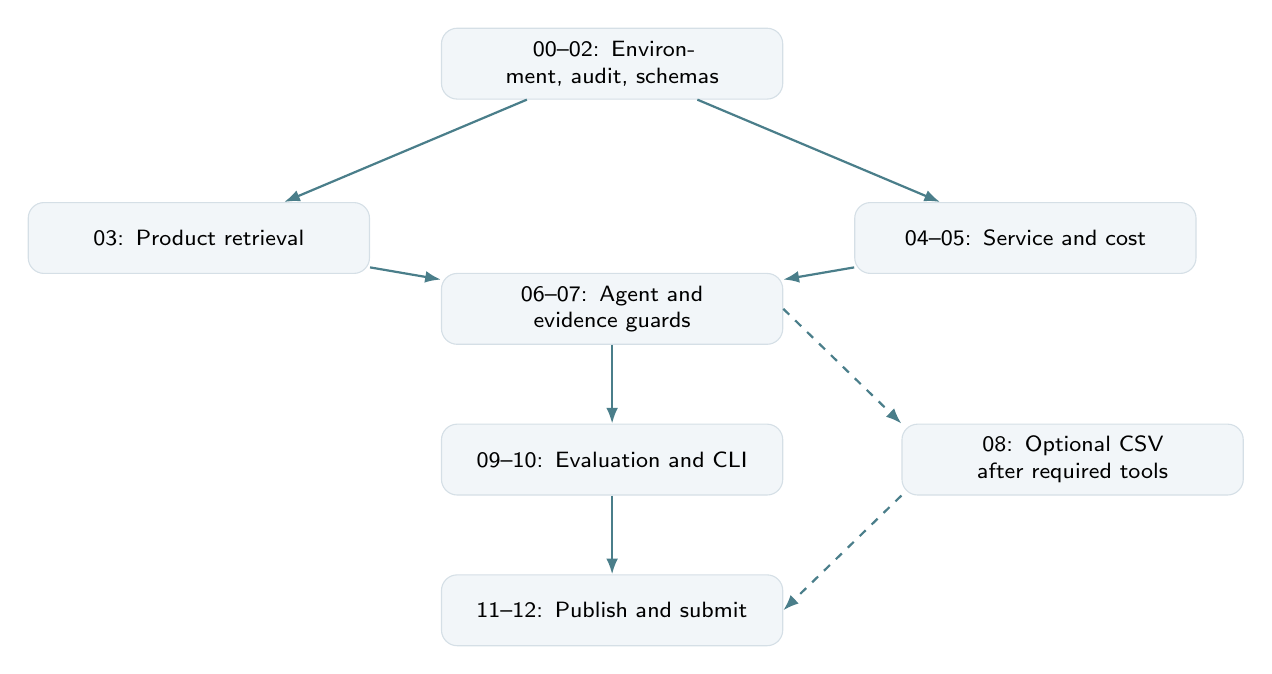
\begin{tikzpicture}[node distance=7mm and 9mm, every node/.style={font=\sffamily\footnotesize},
  B/.style={draw=Rule,rounded corners=2mm,fill=Pale,minimum height=9mm,text width=41mm,align=center},
  A/.style={-{Latex[length=2mm]},draw=Sea,thick}]
\node[B] (a) {00--02: Environment, audit, schemas};
\node[B,below left=13mm and 9mm of a] (b) {03: Product retrieval};
\node[B,below right=13mm and 9mm of a] (c) {04--05: Service and cost};
\node[B,below=22mm of a] (d) {06--07: Agent and evidence guards};
\node[B,below=10mm of d] (e) {09--10: Evaluation and CLI};
\node[B,below=10mm of e] (f) {11--12: Publish and submit};
\draw[A] (a) -- (b);\draw[A] (a) -- (c);
\draw[A] (b) -- (d);\draw[A] (c) -- (d);
\draw[A] (d) -- (e);\draw[A] (e) -- (f);
\node[B,right=15mm of e] (g) {08: Optional CSV\ after required tools};
\draw[A,dashed] (d.east) -- (g.north west);
\draw[A,dashed] (g.south west) -- (f.east);
\end{tikzpicture}
\end{center}
The brochure and service pipelines can be implemented and tested independently after shared schemas exist. The optional CSV analysis may be written as a separate deterministic tool, but it must never delay completion of the required product and cost workflows. The final regression pass and the demonstration require the integrated system.

\subsection{My concrete artifact checklist and sign-off table}
\begin{longtable}{@{}L{12mm}L{54mm}L{77mm}@{}}
\toprule\textbf{Stage} & \textbf{Artifact or file to create} & \textbf{Objective sign-off evidence}\\\midrule\endfirsthead
\toprule\textbf{Stage} & \textbf{Artifact or file to create} & \textbf{Objective sign-off evidence}\\\midrule\endhead
00 & \code{pyproject.toml}, \code{.gitignore}, \code{.env.example} & Working interpreter and Git privacy inspection.\\
01 & \code{scripts/inventory.py}; private inventory and issue log & Counts 12+12 brochures, 50 FSRs, 4097-by-24 CSV and known anomalies.\\
02 & \code{schemas.py}; \code{test_schemas.py} & Invalid and unknown fields handled without invented defaults.\\
03 & Brochure loader and retrieval module & Filter Optimizer page evidence retrieved for the product scenario.\\
04 & Service parser; private evidence ledger & FSR-0027 truncation and discrepancies flagged; other FSRs classified.\\
05 & Cost calculator; \code{test_costs.py} & Reconstructed EUR 2,215.40 clearly labelled; no mixed-currency totals.\\
06 & Agent/controller, tool schemas, session state & Both mandatory prompts route automatically; short follow-up works.\\
07 & Citation and numerical guards & Unsupported specification, price and fake citation blocked.\\
08 & Optional CSV analyzer; \code{test_flotation.py} & Empirical counts 981, 1142, 823 reproduced from data.\\
09 & Private golden-query set; evaluation results & Arithmetic passes, routes measured, failures reported honestly.\\
10 & \code{cli.py} and \code{main.py} & Live CLI with traces, conversation and graceful termination.\\
11 & Final README; public code-only URL & Fresh setup reproducible; data and secrets absent from Git history.\\
12 & Walkthrough; code and video URLs; Recright & Both public links play/open and the interview is submitted.\\
\bottomrule
\end{longtable}

\subsection{My daily working routine and decision rules}
At the start of each session, I will read the current Git status, the latest failing test and the pending stage's exit gate. I will implement the smallest change that satisfies the stage, run its targeted tests, then run the broader suite after any cross-module change. At the end of the session, I will write a brief note recording files changed, tests passed, remaining issues and the next stage. I will never mark a stage complete simply because a file exists; only a passing observable behavior counts.

\textbf{Fallback priorities.} If semantic retrieval adds complexity but not measured quality, keep lexical retrieval. If service-report extraction is imperfect, manually verify a limited set of relevant reports rather than pretending all 50 have clean costs. If the LLM API is temporarily unavailable, preserve offline tool tests and resolve access before recording. If time becomes constrained, skip optional flotation, fancy formatting and nonessential abstractions; stabilize and submit the mandatory demonstrable paths first.

\begin{keybox}
\textbf{Overall definition of done.} The agent is ready only when a salesperson can type natural-language product and service questions; the program chooses relevant tools without manual mode switching; evidence and arithmetic are traceable; unknown product capabilities, missing rates and incompatible currencies do not become invented answers; the code-only public artifact is safe; and both the recorded walkthrough and five-question Recright interview are completed by the employer's deadline.
\end{keybox}

\subsection{Part III conclusion: from a design to a defensible implementation}
My chosen workflow turns the Metso problem into a series of observable engineering decisions: first protect and inspect the evidence, then type it, retrieve it, calculate from it, orchestrate the tools, verify the claims, test beyond the sample prompts, and only then demonstrate the result. The quality of the work will be measured by accurate sourcing, reliable calculations, honest limitations, independent tool routing and reproducibility---not by an elaborate user interface or an unnecessarily large technology stack.

\vspace{5mm}
\begin{center}
{\sffamily\color{Gray}\footnotesize END OF PART III -- THE STEPS I HAVE PLANNED TO COMPLETE THIS PROJECT}\\[2mm]
{\sffamily\bfseries\color{Navy}AG is your G!}
\end{center}


\clearpage
\section{Step One --- Stage 01: Comprehensive Data Audit}
\begin{center}
{\sffamily\large\bfseries\color{Blue}Step One --- Stage 01: Comprehensive Data Audit}\par
{\small\color{Gray}An executable, traceable audit of every authorized Metso data source}
\end{center}

\begin{keybox}
\textbf{Purpose of this new chapter.} This chapter converts the Stage 01 plan from Parts II and III into a reproducible hands-on procedure tailored to my existing Windows project. It explains how to account for every brochure, every field-service report, and the optional flotation CSV; how to preserve the original evidence; and how to identify limitations before building retrieval or cost-estimation components. It is intended as an execution manual and sign-off checklist, not a claim that Stage 01 has already been run.
\end{keybox}

\subsection{Where I actually am: verified progress versus pending checks}
\textbf{Verified from my Windows PowerShell output (17 October 2026).} The selected root is a real directory under my job-application folder ending in \code{interview/project}. Python 3.12.4, Git 2.45.2, and VS Code 1.142.0 are available. The project has an isolated \code{.venv} environment with pip 26.2.1; its editable installation was corrected from an initial unintended 0.0.0 install to \code{metso-sales-agent==0.1.0}. The \code{metso-agent.exe} entry point executes successfully, detects the raw-data directory, and prints ``Stage 00 smoke test passed!'' Pytest ran one collected test and reported \textbf{1 passed in 0.14 seconds}. These checks demonstrate a working scaffold, not a functioning product or service AI agent.

\begin{tabularx}{\textwidth}{@{}L{51mm}L{27mm}Y@{}}
\toprule\textbf{Activity} & \textbf{Status} & \textbf{Evidence / limitation}\\\midrule
Python environment and CLI entry point & Confirmed & Python 3.12.4; \code{metso-agent.exe} runs.\\
Source folders available locally & Partly confirmed & One brief, 12 Markdown brochures, 12 corresponding PDFs, and 50 service reports identified by count; existence of the expected raw-data folder confirmed.\\
Unit-test runner & Confirmed & \code{tests/test_smoke.py}: one passing test; it tests importability, not document correctness.\\
Git confidentiality review & \textbf{Pending} & No final \code{git check-ignore}, \code{git status}, or \code{git ls-files} proof has yet been supplied.\\
Comprehensive Stage 01 audit & \textbf{Not executed} & This chapter specifies the audit and outputs; successful audit results should be filled in only after running the scripts.\\
Product RAG, cost engine, routing agent & Not built & Planned for later stages and never to be represented as tested here.\\
\bottomrule
\end{tabularx}

\subsection{The actual on-disk layout used in this project}
I will use the current \code{project/} directory \emph{itself} as the Python and Git repository root; I will not introduce an extra nested \code{metso-sales-agent/} directory. My original input files are already extracted under \code{raw/}. They should remain immutable source evidence. The code will read from \code{raw/data/} rather than from the \code{data/} path shown in the original ZIP.
\begin{Verbatim}[fontsize=\footnotesize]
project/
  raw/                            # CONFIDENTIAL; never publish
    candidate-brief.md
    data/
      brochures/                  # 12 x .md and 12 x .pdf
      HistoricalServices/         # 50 x FSR-NNNN.txt
      flotation_process_data_hourly.csv
  src/metso_agent/                # existing Python package
    __init__.py
    cli.py
  tests/test_smoke.py             # existing first unit test
  scripts/                        # create at Stage 01
    inventory.py
  docs/                           # share sanitized methods only
    private/                      # confidential reviews, ignored
  local_cache/audit/              # private machine-readable outputs
  logs/                           # private runtime logs
  .venv/                          # local interpreter and packages
  .gitignore
  .env.example
  pyproject.toml
\end{Verbatim}
\textbf{Why location matters.} Relative paths in Python will be derived using \code{Path(__file__).resolve()} and the project root. For example, \code{RAW_DATA_DIR=raw/data} points to \code{project/raw/data/}. Re-extracting the ZIP into \code{project/data/} is unnecessary and risks creating competing copies.

\subsection{Stage 01 must begin with a confidentiality gate}
The employer expressly prohibits including its \code{data/} materials in public code submissions, and the email labels attachments \emph{RESTRICTED}. Before generating an inventory or committing code, I must check the ignore configuration. A private report containing customer sites, historical rates or direct source excerpts must stay outside any public Git history, and copied raw PDF/ZIP/report files must not remain unignored in the root.

\begin{Verbatim}[fontsize=\footnotesize]
# Windows PowerShell; run from the existing project/ root
Get-Location
Test-Path .\raw\candidate-brief.md
Test-Path .\raw\data\flotation_process_data_hourly.csv
# inspect .gitignore; it must cover at least:
# raw/  .venv/  .env  local_cache/  docs/private/
# logs/  .pytest_cache/  *.egg-info/
git init
git check-ignore -v raw/candidate-brief.md
git check-ignore -v raw/data/brochures/filter-optimizer.md
git status --short --ignored
git ls-files
\end{Verbatim}

\begin{warnbox}
\textbf{Do not stage or publish until the check passes.} If \code{git ls-files} already lists private files, adding an ignore rule is insufficient: Git must stop tracking them, and the history must be reviewed before any public push. The original ZIP and private analytical PDF/TeX reports should be kept inside an ignored private location (for example \code{raw/}), or covered by explicit additional ignore rules. The \code{docs/} folder is not automatically private; use \code{docs/private/} for raw-derived observations.
\end{warnbox}

\subsection{The audit question and the three evidence domains}
Stage 01 is a \textbf{descriptive inspection}, not model training, retrieval ranking, cost prediction or a source-cleaning rewrite. It answers: ``Exactly what information was supplied? Which files and fields can support which later questions? Where is that information incomplete, inconsistent or ambiguous?''
\begin{tabularx}{\textwidth}{@{}L{36mm}L{46mm}Y@{}}
\toprule\textbf{Source} & \textbf{Later allowable claim} & \textbf{Main audit concern}\\\midrule
\code{brochures/*.md,pdf} & Product capabilities and specifications & Missing pages, flattened technical tables, model differences and correct page attribution.\\
\code{FSR-*.txt} & Historical task evidence, rates, parts and service costs & Missing invoices, inconsistent times, mixed currencies, bundled work and truncated records.\\
\code{flotation*.csv} & Historical concentration and process statistics & Data types, missing cells, duplicate timestamps, time gaps, units absent from headers.\\
\code{candidate-brief.md} & Binding task instructions & Whether every mandatory behavior, restriction and deliverable is carried through.\\
\bottomrule
\end{tabularx}

\subsection{01.1 --- Establish a read-only baseline and manifest}
\begin{enumerate}
\item \textbf{Capture the source boundary.} Confirm \code{candidate-brief.md} lives in \code{raw/} and confirm brochure, FSR and CSV subdirectories are present. Preserve their file names exactly; do not rename or edit the originals.
\item \textbf{Count and classify.} Expected baseline from the provided source package: 1 brief + 24 brochure files + 50 FSR text files + 1 CSV = \textbf{76 actual files}. The archive also contained three folder entries, which must not be counted as files.
\item \textbf{Hash every source.} Calculate SHA-256 checksums so that a later processing step can demonstrate that its input corresponds to the same original file. A hash does not validate semantic correctness; it validates byte identity.
\item \textbf{Record reproducibility metadata.} Include the relative source path, file extension, file size, and hash. It is sensible to include modification time for diagnostics, but file modification time must not be assumed to be the field-visit date.
\item \textbf{Report exceptions.} Unexpected files, duplicate names, absent expected IDs, empty files or unreadable text must produce explicit issues; do not silently skip them.
\end{enumerate}
\textbf{Planned artifact:} \code{local_cache/audit/data_inventory.json}; generated by \code{scripts/inventory.py}. The inventory stays private and can be regenerated from the locally authorized source materials.

\subsection{01.2 --- Brochure audit: all 12 PDF/Markdown pairs}
\subsubsection{Inventory and pairing rules}
For every \code{*.md} under \code{raw/data/brochures/}, a PDF with the same stem should exist. Use sets of \code{Path.stem} values to detect missing counterparts. Two different source documents can address the same product family: \code{larox-pf-brochure-a} and \code{larox-pf-brochure-b} must not be merged or falsely counted as independent products.

\begin{longtable}{@{}L{50mm}L{13mm}L{81mm}@{}}
\toprule\textbf{Brochure stem} & \textbf{Pages} & \textbf{Main coverage to verify}\\\midrule\endfirsthead
\toprule\textbf{Brochure stem} & \textbf{Pages} & \textbf{Main coverage to verify}\\\midrule\endhead
\code{ac-filter} & 2 & Solvent/organic polishing of process solutions.\\
\code{cellstation} & 3 & Air and pulp-level control for flotation cells.\\
\code{columncell} & 4 & Column flotation processes and claims.\\
\code{concorde-cell} & 12 & High-intensity flotation of fine and ultrafine material.\\
\code{filter-optimizer} & 4 & Changing feed conditions and filtration setpoint optimization.\\
\code{floatforce-upgrade} & 3 & Rotor/stator mixing mechanism upgrade.\\
\code{gm-filter} & 1 & Coalescing removal of insoluble organics.\\
\code{larox-pf-brochure-a} & 8 & General Larox PF family operation.\\
\code{larox-pf-brochure-b} & 12 & More detailed Larox PF series and specifications.\\
\code{larox-pf-ds} & 8 & Double-sided tower press and cloth arrangement.\\
\code{md-series-pump} & 4 & Mill-discharge slurry pumps.\\
\code{orion-series-pump} & 12 & Horizontal slurry pumps and configurations.\\
\midrule\textbf{Total labeled Markdown pages} & \textbf{73} & Baseline documented in the prior analysis; audit must recompute.\\
\bottomrule
\end{longtable}

\subsubsection{Page and content integrity}
\begin{enumerate}
\item Identify explicit Markdown page markers (the supplied extractions use headings such as \code{#### Page 2}). Verify page numbers form the expected sequence, with no missing or duplicate labels.
\item Record the first and last marker and number of pages per document. Where possible, compare with the original PDF page count. If PDF parsing libraries are unavailable, first flag the PDF check as pending instead of asserting the counts match.
\item Sample technical tables in \code{larox-pf-brochure-b} and \code{larox-pf-ds}; inspect the PDF layout to verify any numeric values flattened by Markdown extraction.
\item Record title, product family, canonical document ID, aliases, source file and per-page location. Do not correct a suspicious number in the original Markdown; add an issue and reference the source PDF.
\item Create a small gold set of reliable page references that a future retrieval component should find. This is \emph{audit evidence}, not a preprogrammed answer to the final customer prompt.
\end{enumerate}

\begin{examplebox}
\textbf{Priority product cross-check (previously identified, requiring confirmation in this run).} The Filter Optimizer brochure, especially pages 2--3, describes adapting filtration setpoints to changing process conditions. The PF-DS brochure describes an endless filter cloth, whereas some FSRs count replacement of multiple ``cloths.'' This terminology conflict should be recorded now, without resolving it through assumption.
\end{examplebox}

\subsection{01.3 --- Field-service audit: all 50 FSR files}
\subsubsection{Completeness and classification}
Expected names are \code{FSR-0001.txt} through \code{FSR-0050.txt}, with no missing or duplicate identifiers. A report may have itemized costs, a single bundled total, narrative work descriptions, or no actual price. Its cost availability must be classified independently of whether the service description is useful.

\begin{tabularx}{\textwidth}{@{}L{40mm}Y@{}}
\toprule\textbf{Status} & \textbf{Audit meaning}\\\midrule
\code{ITEMIZED_COST} & Quantity and rate/amount evidence for separable line items is present.\\
\code{BUNDLED_TOTAL} & A total price is reported, but individual services or parts cannot be reliably isolated.\\
\code{PARTIAL_COST} & Only some components are priced or a table/statement is cut off.\\
\code{UNPRICED} & ``Invoice to follow,'' ``as per agreement'' or no monetary amount. Not a free visit.\\
\code{AMBIGUOUS} & Conflicting or unclear quantities, units, rates or totals need manual review.\\
\bottomrule
\end{tabularx}

\subsubsection{Record-level fields to inspect}
For each report retain these field groups with a corresponding source line or source span whenever extraction becomes automated:
\begin{itemize}
\item \textbf{Identity:} report ID, date, country, customer, site, technician/report style.
\item \textbf{Equipment and action:} model, inspected equipment, intended activities versus completed activities, number of units replaced, secondary tasks.
\item \textbf{Timing:} reported on-site hours, billable labor hours, travel hours, arrival/departure time, sums of listed activity durations.
\item \textbf{Monetary:} currency, labor and travel rates, parts quantities and prices, consumables, printed line totals, printed subtotal, tax and final total.
\item \textbf{Evidence quality:} approximate language, contradictions, truncation, missing prices, bundled repair scope, tax inclusion and unit ambiguity.
\end{itemize}

\subsubsection{Priority manual review queue}
\begin{longtable}{@{}L{23mm}L{54mm}L{67mm}@{}}
\toprule\textbf{Report} & \textbf{Relevance} & \textbf{Known risk to recheck}\\\midrule\endfirsthead
\toprule\textbf{Report} & \textbf{Relevance} & \textbf{Known risk to recheck}\\\midrule\endhead
\code{FSR-0027} & PF-DS 12-cloth replacement, Sweden & Truncated cost summary; stated 8.4 h versus 8.75 h elapsed activity window.\\
\code{FSR-0014} & PF-DS 16-cloth case, Canada & Additional hydraulic/nozzle work and CAD price.\\
\code{FSR-0031} & PF-DS 24-cloth case, Finland & Broader scope, EUR unit price variation and VAT.\\
\code{FSR-0028} & Incomplete cloth replacement & Intended scope differs from completed scope; no verified fee.\\
\code{FSR-0001} & Chile local-rate context & ColumnCell task; not a PF-DS cloth replacement.\\
\code{FSR-0015} & Chile local-rate context & Filter Optimizer hardware included in total.\\
\code{FSR-0034} & Chile local-rate context & ColumnCell maintenance, different scope.\\
\code{FSR-0035} & Chile local context & Bundled USD amount; no separable rates.\\
\code{FSR-0046} & Chile local context & Agreement-based pricing absent from text.\\
\bottomrule
\end{longtable}

\begin{warnbox}
\textbf{The FSR-0027 arithmetic is an example of why auditing precedes estimation.} The previously reviewed line items reconstruct EUR~2,215.40 when using the report's 8.4 on-site hours. Its 07:30--16:15 window spans 8.75 hours, and changing the labor assumption would produce EUR~2,242.70. Neither value is a source-printed, complete invoice, and neither is a Chile quote. Stage 01 must record the discrepancy; Stage 05 will eventually decide how to present supported cost components.
\end{warnbox}

\subsection{01.4 --- Flotation CSV audit: structure, time and units}
The optional CSV is still relevant for understanding source coverage even if the optional tool is deferred. The existing report identifies \textbf{4,097 rows and 24 columns}, with a date column and 23 numeric fields. This is the expected baseline and must be recomputed locally.

\begin{enumerate}
\item Check file readability, encoding and delimiter. Print original column names before attempting any normalization.
\item Verify exact dimensions; inspect dtypes, missing values, failed numeric conversions and duplicate complete rows.
\item Parse the original timestamp string with an explicit verified format. Inspect duplicate timestamps, sorting, expected one-hour intervals and all gaps greater than one hour.
\item Retain the original precision. Do not assume that reagent/air flows and column levels have a particular physical unit when the header does not state one.
\item Profile \texttt{\% Iron Concentrate} and \texttt{\% Silica Concentrate} with mean, median, minimum, maximum, quantiles and threshold counts; do not label these operational readings as contractual limits.
\item Keep the statistics in the local audit output, explicitly labeled as \emph{computed from the file}. They should not be presented as proof of a model, diagnosis or causal mechanism.
\end{enumerate}

\begin{tabularx}{\textwidth}{@{}L{54mm}L{27mm}Y@{}}
\toprule\textbf{Check} & \textbf{Prior baseline} & \textbf{What counts as passing}\\\midrule
Rows / columns & 4,097 / 24 & Direct CSV load gives same shape.\\
Null cells & 0 & Recompute; flag if nonzero.\\
Duplicate complete rows & 0 & Recompute and record separately from duplicate timestamps.\\
Observed time coverage & Mar--Sep 2017 & Parse date column explicitly and inspect extremes.\\
Known gap & 13 d 7 h & Identify the interval in consecutive timestamp differences.\\
Joint example threshold & 823 / 4,097 & Independently recomputed only if the optional numeric check is enabled.\\
\bottomrule
\end{tabularx}

\subsection{01.5 --- Issue register and severity policy}
Each anomaly should be written to a local machine-readable log rather than corrected in place. A minimal issue record includes \code{issue_id}, \code{source_path}, \code{category}, \code{severity}, \code{observed_evidence}, \code{why_it_matters}, \code{action}, and \code{review_status}.

\begin{tabularx}{\textwidth}{@{}L{22mm}L{55mm}Y@{}}
\toprule\textbf{Severity} & \textbf{Interpretation} & \textbf{Example}\\\midrule
\textbf{Critical} & Prevents a supported calculation or makes an identity uncertain. & Unsupported monetary rate, missing source file, cross-currency arithmetic.\\
\textbf{High} & Could materially change a product or service recommendation. & Conflicting PF-DS cloth units; truncated FSR-0027; inconsistent hours.\\
\textbf{Medium} & Limits coverage or reduces precision without necessarily blocking use. & Flattened table; missing nonessential metadata; undocumented units.\\
\textbf{Low} & Mainly documentation or formatting issue. & Inconsistent report headings or date presentation if parseable.\\
\bottomrule
\end{tabularx}

\begin{examplebox}
\textbf{Example private issue record (illustrative, not automatically generated):} \code{ID=FSR-0027-HOURS-01}; source \code{FSR-0027.txt}; category \code{HOURS_CONFLICT}; severity \code{HIGH}; observed 8.4 reported hours versus 8.75 elapsed hours; action: preserve both values, avoid selecting one as indisputable billable time.\par
\textbf{Do not mark this record resolved} until a reviewer verifies the original fields and explicitly decides what downstream use is allowed.
\end{examplebox}

\subsection{01.6 --- Implement the first repeatable inventory script}
I will introduce \code{scripts/inventory.py} as a minimal \emph{read-only} collector. It will use Python's standard library plus already installed Pandas, compute file hashes, check brochure and FSR naming, count Markdown page markers, inspect the CSV dimensions, and save a structured manifest to \code{local_cache/audit/}. Later, dedicated human review and PDF-level verification will add richer findings. The script must never rewrite \code{raw/}.

\begin{Verbatim}[fontsize=\scriptsize]
# scripts/inventory.py -- read-only Stage 01 baseline
from pathlib import Path
import hashlib
import json
import re
import pandas as pd

ROOT = Path(__file__).resolve().parents[1]
RAW = ROOT / "raw"
DATA = RAW / "data"
OUT = ROOT / "local_cache" / "audit"
PAGE = re.compile(r"^#{1,6}\s*Page\s+(\d+)\s*$", re.M)


def sha256(path: Path) -> str:
    digest = hashlib.sha256()
    with path.open("rb") as stream:
        for block in iter(lambda: stream.read(65536), b""):
            digest.update(block)
    return digest.hexdigest()


def record(path: Path) -> dict:
    return {
        "path": str(path.relative_to(ROOT)).replace("\\", "/"),
        "bytes": path.stat().st_size,
        "sha256": sha256(path),
    }


def main() -> None:
    brochures = DATA / "brochures"
    reports = DATA / "HistoricalServices"
    csv_file = DATA / "flotation_process_data_hourly.csv"
    brief = RAW / "candidate-brief.md"
    required = [brief, brochures, reports, csv_file]
    missing = [str(p) for p in required if not p.exists()]
    if missing:
        raise SystemExit(f"Required sources missing: {missing}")

    md = sorted(brochures.glob("*.md"))
    pdf = sorted(brochures.glob("*.pdf"))
    fsr = sorted(reports.glob("FSR-*.txt"))
    md_ids = {p.stem for p in md}
    pdf_ids = {p.stem for p in pdf}
    expected = {f"FSR-{i:04d}" for i in range(1, 51)}
    actual = {p.stem for p in fsr}

    pages = {}
    for path in md:
        txt = path.read_text(encoding="utf-8-sig")
        pages[path.stem] = [int(n) for n in PAGE.findall(txt)]

    df = pd.read_csv(csv_file)
    sources = [brief, *md, *pdf, *fsr, csv_file]
    manifest = {
        "counts": {
            "markdown": len(md), "pdf": len(pdf),
            "reports": len(fsr), "csv_rows": len(df),
            "csv_columns": len(df.columns),
            "all_actual_files": len(sources),
        },
        "unpaired_markdown": sorted(md_ids - pdf_ids),
        "unpaired_pdf": sorted(pdf_ids - md_ids),
        "missing_fsr": sorted(expected - actual),
        "unexpected_fsr": sorted(actual - expected),
        "pages_by_brochure": pages,
        "csv_columns": df.columns.tolist(),
        "csv_missing_cells": int(df.isna().sum().sum()),
        "files": [record(p) for p in sources],
    }
    OUT.mkdir(parents=True, exist_ok=True)
    target = OUT / "data_inventory.json"
    target.write_text(json.dumps(manifest, indent=2),
                      encoding="utf-8")
    print(json.dumps(manifest["counts"], indent=2))
    print(f"PRIVATE inventory saved: {target}")


if __name__ == "__main__":
    main()
\end{Verbatim}

\begin{warnbox}
\textbf{Correct interpretation of this script.} It is a \emph{starter inventory}, not a complete forensic audit. It does not validate PDF numerical tables, parse all cost components, classify FSR billing reliability, or confirm timestamp parsing. Those tasks require the manual and follow-on checks specified in this chapter. A successfully written JSON file does not prove every source is semantically correct.
\end{warnbox}

\subsection{01.7 --- Run the inventory and verify its first output}
Create the folder and file in VS Code, save the code above, then execute from the actual \code{project/} root:
\begin{Verbatim}[fontsize=\footnotesize]
New-Item -ItemType Directory -Force -Path .\scripts
.\.venv\Scripts\python.exe .\scripts\inventory.py
Get-Content .\local_cache\audit\data_inventory.json |
    Select-Object -First 25
\end{Verbatim}
\begin{tabularx}{\textwidth}{@{}L{55mm}L{26mm}Y@{}}
\toprule\textbf{Inventory field} & \textbf{Target} & \textbf{If the value differs}\\\midrule
\code{markdown} & 12 & Verify expected brochure location and extensions.\\
\code{pdf} & 12 & Investigate missing/misnamed PDF pairs.\\
\code{reports} & 50 & Investigate unexpected numbering or nested folders.\\
\code{csv_rows} & 4097 & Check parser, extra header rows and source version.\\
\code{csv_columns} & 24 & Inspect delimiter and duplicate/unnamed headers.\\
\code{all_actual_files} & 76 & Verify the complete expected package files.\\
\code{unpaired_markdown/pdf} & Empty lists & Review stems without renaming originals.\\
\code{missing_fsr} & Empty list & Check the sequential 0001--0050 identifiers.\\
\bottomrule
\end{tabularx}

\textbf{Important:} If counts are correct, only the \emph{structural inventory} passes. Still inspect the page-marker lists for all 12 Markdown files and manually verify at least the priority PDF tables and cost reports.

\subsection{01.8 --- Follow-on CSV profiling commands}
The inventory code establishes CSV shape and missing cells. The next focused inspection should examine timestamps, duplicate rows and historical thresholds. A short private notebook or script can begin as follows (confirm the actual date representation before locking a strict parser format):
\begin{Verbatim}[fontsize=\footnotesize]
from pathlib import Path
import pandas as pd

p = Path("raw/data/flotation_process_data_hourly.csv")
df = pd.read_csv(p)
print("Shape:", df.shape)
print("Null cells:", int(df.isna().sum().sum()))
print("Duplicate rows:", int(df.duplicated().sum()))
print("Columns:", df.columns.tolist())

# Inspect several raw timestamp strings first.
print(df["date"].head(5).tolist())
# Then select and document a matching explicit date format.
\end{Verbatim}
A separate reviewed step should compute intervals \code{dates.sort_values().diff()}, verify the known time gap, and recompute the optional silica/iron descriptive statistics. This avoids disguising an unverified date-format assumption as an audit result.

\subsection{01.9 --- Manual review procedure for high-risk sources}
\begin{enumerate}
\item \textbf{Open the original and extraction side by side.} Use the PDF to assess brochure tables and the TXT to assess report monetary statements. Avoid optical character recognition unless a source is genuinely unreadable.
\item \textbf{Quote only the minimal necessary fragment in private review notes.} Keep enough context to support the finding while respecting the employer's restricted distribution instruction.
\item \textbf{Verify fields independently.} For cost records compare quantities, currency symbols, explicit rates, multiplication, source-printed totals, on-site activity time and billed time as distinct fields.
\item \textbf{Assign an issue ID and state.} Mark each observation \code{OPEN}, \code{REVIEWED}, or \code{RESOLVED}; never set \code{RESOLVED} merely because a parser produced a number.
\item \textbf{Record permissible downstream use.} A truncated report may be a good task match but only partial cost evidence; a Chilean ColumnCell report may supply country context but not a PF-DS cloth unit price.
\end{enumerate}

\subsection{01.10 --- Deliverables, naming and safe storage}
\begin{longtable}{@{}L{51mm}L{23mm}L{69mm}@{}}
\toprule\textbf{Artifact} & \textbf{Visibility} & \textbf{Purpose}\\\midrule\endfirsthead
\toprule\textbf{Artifact} & \textbf{Visibility} & \textbf{Purpose}\\\midrule\endhead
\code{scripts/inventory.py} & Public-safe code & Reproducible scan of local authorized files; no embedded Metso data.\\
\code{tests/test_inventory.py} & Public-safe code & Synthetic fixtures for names, hash stability and count/flag behavior.\\
\code{data_inventory.json} & \textbf{Private} & Full source list, hashes, count and page metadata.\\
\code{data_quality_issues.json} & \textbf{Private} & Structured missing/conflicting/uncertain source findings.\\
\code{docs/private/data_audit.md} & \textbf{Private} & Human-readable audit memo with source-specific evidence notes.\\
\code{docs/audit_methodology.md} & Public-safe & Method, command examples and generic quality checks without restricted content.\\
\bottomrule
\end{longtable}
A privacy review is required even for apparently harmless metadata. File names, customer locations and historical amounts may be sensitive when combined. Do not assume a generated summary is automatically safe to publish simply because it is not a raw \code{.txt} or \code{.pdf}.

\subsection{01.11 --- Test plan for the audit itself}
A trustworthy audit also needs tests. The first small \code{pytest} suite should check the following with \emph{synthetic temporary files} so it can run on a clean clone without the Metso data:
\begin{enumerate}
\item \textbf{Pairing test:} matching \code{alpha.md} and \code{alpha.pdf} gives no missing counterpart; a missing PDF is flagged.
\item \textbf{FSR identifier test:} expected names in a synthetic range reveal omissions and unexpected names without treating a different equipment label as a filename error.
\item \textbf{Hash stability test:} identical file bytes yield the same SHA-256; changing one byte changes the hash.
\item \textbf{Page-marker test:} explicit \code{#### Page 1} and \code{#### Page 2} are recognized, while repeated or missing markers are surfaced by validation.
\item \textbf{Missing-file failure:} absent \code{candidate-brief.md} or CSV produces a clear error rather than a false successful audit.
\item \textbf{Read-only behavior:} source checksums before and after the inventory are unchanged.
\item \textbf{Privacy test:} generated manifest is placed in the ignored local-cache path, not in an unignored \code{docs/} directory.
\end{enumerate}
The existing \code{tests/test_smoke.py} remains a separate test of the installed CLI package. Its successful result must not be counted as an audit correctness test.

\subsection{01.12 --- Stage 01 decision gate: when may I proceed to Stage 02?}
\begin{tabularx}{\textwidth}{@{}L{12mm}L{105mm}Y@{}}
\toprule\textbf{ID} & \textbf{Required observation} & \textbf{Sign-off}\\\midrule
G01 & Git ignores \code{raw/}, caches, credentials and private reports; no sensitive tracked paths. & Pending\\
G02 & One candidate brief and exactly 76 expected actual source files accounted for. & Pending\\
G03 & Twelve PDF/Markdown brochure stems pair correctly and page marker issues are logged. & Pending\\
G04 & All 50 FSR IDs exist; each is provisionally classified by cost evidence status. & Pending\\
G05 & FSR-0027 truncation/hour discrepancy, PF-DS cloth ambiguity and currency/tax risks are logged. & Pending\\
G06 & CSV structure, nulls, duplicates, chronological gaps and column units are checked. & Pending\\
G07 & Private JSON inventory and issue register exist, with reproducible code and source checksums. & Pending\\
G08 & A human-readable private audit summary states what evidence can and cannot justify. & Pending\\
G09 & Synthetic unit tests for the inventory pass; no original source bytes are modified. & Pending\\
\bottomrule
\end{tabularx}
\begin{keybox}
\textbf{Definition of done for Stage 01.} I can account for each authorized source file, explain its scope, identify the principal quality defects and trace audit results to the unchanged raw materials. The outputs are local, reproducible and safe from accidental public inclusion. Only then should Stage 02 formalize Pydantic \code{ProductEvidence}, \code{ServiceReport}, \code{CostItem} and other schemas based on facts uncovered here. The table above intentionally remains \emph{Pending}: this document is the audit plan, not a fictional execution log.
\end{keybox}

\subsection{01.13 --- First working session: precise order of actions}
\begin{enumerate}
\item Run the Git ignore/tracking commands from the actual \code{interview/project} root. Fix any privacy problem before staging files.
\item Confirm the existing \code{raw/} file paths and run a four-item PowerShell count check (Markdown, PDF, FSR and CSV presence).
\item Create \code{scripts/} and save \code{inventory.py} above. Run it with \code{.venv/Scripts/python.exe}.
\item Inspect the JSON counts, all 12 document stems, page-marker sequences and all 50 FSR IDs. Record any mismatch in the issue register rather than modifying source files.
\item Run focused CSV metadata and timeline profiling. Record null/duplicate/gap checks and original header names.
\item Review the priority brochure PDFs and FSR reports manually. Record high-severity risks with evidence pointers.
\item Write a private Stage 01 sign-off note: checks performed, observed findings, outstanding uncertainties, tests executed and readiness for Stage 02.
\end{enumerate}

\begin{warnbox}
\textbf{Final boundary.} This chapter does not authorize publishing the supplied Metso documents, full report excerpts, price lists or customer-site data. It does not replace the employer's roughly four-hour suggested implementation scope. The practical goal is to protect the evidence and produce only the audit depth needed to make the two mandatory workflows reliable before the 20 October deadline.
\end{warnbox}

\vspace{4mm}
\begin{center}
{\sffamily\color{Gray}\footnotesize END OF PART IV -- STAGE 01 DATA AUDIT EXECUTION GUIDE}\\[2mm]
{\sffamily\bfseries\color{Navy}AG is your G!}
\end{center}

\clearpage
\section{Step Two --- Stage 02: Design Typed Data Contracts and Evidence Provenance}
\begin{center}
{\sffamily\large\bfseries\color{Blue}Implementation Evidence, Validation Rules, and Verified Test Results}\par
{\small\color{Gray}An engineering execution record for the Metso AI Sales Assistant Agent, 17 October 2026}
\end{center}

\begin{keybox}
\textbf{Chapter objective.} Document exactly what was performed in Stage 02, why typed schemas and provenance matter for the assignment, what was proven by local PowerShell and Pytest output, and which contractual safeguards still require implementation. This is a \emph{verified foundation report}, not an assertion that the complete AI agent, service parser, retrieval pipeline, or comprehensive data audit is finished.\\[3pt]
\textbf{Primary evidence.} The developer's supplied Windows PowerShell transcript shows Python 3.12.4, Pydantic 2.14.1, Git initialization and ignore checks, thirteen passing schema tests, fourteen passing full-suite tests, and successful instantiation of a source-reference object. These are the observed results described below. They were reported by the developer; this report did not directly execute commands on the developer's Windows machine.
\end{keybox}

\subsection{Scope, sequencing, and the exact state at the start of Stage 02}
Stage 02 is the \term{typed-data and provenance layer} between unstructured evidence and downstream AI tools. Product brochures are page-oriented technical documents; service reports are semi-structured accounts of technician activities and charges; the optional flotation CSV contains time-indexed measurements. They cannot safely be handled as indistinguishable free-form strings when the system must support auditable claims and cost calculations.

In the intended project sequence, Stage 01 first inspects the corpus and registers its quality issues. Stage 02 then defines the contracts that parsers, search tools, calculators and the response composer will exchange. In actual development, the developer began implementing the independent Stage 02 schemas before providing proof that the complete Stage 01 inventory script and issue register had been executed. \textbf{This dependency remains open.} Passing schema tests does not establish that all 50 reports were parsed or that the CSV was profiled.

\begin{tabularx}{\textwidth}{@{}L{41mm}L{24mm}Y@{}}
\toprule\textbf{Component} & \textbf{Observed status} & \textbf{Evidence and appropriate interpretation}\\\midrule
Python environment & Confirmed & Python 3.12.4 inside the dedicated \code{.venv}; installation check for Pydantic succeeds.\\
Schema implementation & Confirmed by tests & \code{tests/test_schemas.py} imported the expected types and passed 13 tests.\\
Full test runner & Confirmed & Pytest collected 14 tests; all 14 passed.\\
Local Git repository & Confirmed & \code{git init} created the \code{.git} directory.\\
Ignored source folder & Confirmed & \code{git check-ignore} resolved \code{raw/} via \code{.gitignore}; private files were moved inside \code{raw/}.\\
Complete Git safety audit & Partial & Ignore status observed; \code{git ls-files}, Git history and \code{.env.example} contents were not shown in the final transcript.\\
Stage 01 full data audit & Not demonstrated & No generated audited inventory, anomaly register, or source-by-source validation logs supplied.\\
Schema design memo & Not demonstrated & No output confirming the presence of \code{docs/data_schema_design.md}.\\
\bottomrule
\end{tabularx}

\subsection{The actual working environment and directory structure}
The implementation runs from the existing \code{interview/project} directory; no extra nested repository root is necessary. The supplied materials are already located below \code{raw/data/}, so future scripts should use that authorized local source location rather than duplicating the original ZIP's \code{data/} directory.

\begin{Verbatim}[fontsize=\footnotesize]
project/
  .git/                       # created with git init (local history)
  .gitignore                  # protects raw/ and local artifacts
  .env.example                # placeholders; inspect before publication
  pyproject.toml              # editable package and test configuration
  .venv/                      # Python 3.12.4 isolated environment
  raw/                        # employer material: ignored by Git
    candidate-brief.md
    AI-Engineer-Task.zip
    Metso_Report_Parts_1_2_3_4.pdf
    Metso_Report_Parts_1_2_3_4.tex
    data/
      brochures/
      HistoricalServices/
      flotation_process_data_hourly.csv
  src/metso_agent/
    __init__.py
    cli.py
    schemas.py                # added for Stage 02
  tests/
    test_smoke.py
    test_schemas.py           # 13 targeted validations
  docs/                       # public-safe methodology only
  local_cache/                # generated confidential data
  logs/                       # local and ignored
\end{Verbatim}
\textbf{Directory status convention.} The tree combines confirmed paths with the intended project arrangement. In particular, the most recent logs prove that \code{schemas.py} is importable through Pytest, not that every documentation file mentioned elsewhere in the plan exists. The names of moved files were demonstrated by the \code{Move-Item} commands and their disappearance from the untracked root listing.

\subsection{Execution chronology: what was run, why, and what changed}
\subsubsection{02.1 --- Confirm the interpreter, validation library, and baseline test}
The developer activated the dedicated virtual environment. These commands established the active toolchain:
\begin{Verbatim}[fontsize=\footnotesize]
.\.venv\Scripts\python.exe --version
.\.venv\Scripts\python.exe -m pip show pydantic
.\.venv\Scripts\python.exe -m pytest -q
\end{Verbatim}
Observed output included \code{Python 3.12.4}, \code{pydantic 2.14.1}, and \code{1 passed in 0.09s}. At this point only the original smoke test was collected. The result showed that the package and basic test runner worked; it did \emph{not} establish the schema implementation yet.

Using the explicit interpreter path makes package resolution reproducible despite other Python versions installed on the machine. Pydantic was selected to validate fields and model invariants at the boundaries between document parsers, pricing logic, and the agent controller.

\subsubsection{02.2 --- Initialize Git, then verify the local confidentiality boundary}
An early attempt to inspect Git status returned \code{fatal: not a git repository}; the developer then executed \code{git init}, creating a local repository. The developer's \code{git check-ignore -v raw/candidate-brief.md} output identified \code{.gitignore:5:raw/}, confirming that this source file was excluded by the ignore rule.

The first Git status showed three sensitive or private study files still untracked in the public-code root: the assignment ZIP, a private PDF report, and its LaTeX source. The developer moved them under the already-ignored \code{raw/} directory. A later status no longer listed those files as untracked, while \code{raw/}, \code{.venv/} and cache paths were shown with \code{!!}, the Git marker for ignored files. This is a \emph{local safety improvement}, not proof that no past commit could ever contain restricted material.

\subsubsection{02.3 --- Diagnose the initial missing-module exception}
The developer first attempted to import \code{metso_agent.schemas} and received:
\begin{Verbatim}[fontsize=\footnotesize]
ModuleNotFoundError: No module named 'metso_agent.schemas'
\end{Verbatim}
A direct file check returned \code{False} for \code{src/metso_agent/schemas.py}, and the directory listing showed only \code{__init__.py}, \code{cli.py} and \code{__pycache__}. Thus the immediate cause was an absent schema source file, \emph{not} a broken Pydantic installation or an unexplained model-library failure.

The developer then added the schema module and the corresponding unit-test module. The later successful tests prove that Python subsequently found and executed those definitions. This is an example of evidence-based debugging: check the filesystem first, correct the missing artifact, then retest without reinstalling the entire environment.

\subsubsection{02.4 --- Execute targeted and whole-project tests}
The developer ran the two relevant test commands:
\begin{Verbatim}[fontsize=\footnotesize]
.\.venv\Scripts\python.exe -m pytest tests/test_schemas.py -v
.\.venv\Scripts\python.exe -m pytest -v
\end{Verbatim}
The targeted command collected 13 tests and reported \textbf{13 passed in 0.53 seconds}. The broader command collected 14 tests and reported \textbf{14 passed in 0.38 seconds}. The full suite comprised those 13 schema tests plus \code{tests/test_smoke.py::test_cli_entrypoint_exists}. No failures or errors were shown in the final test sessions.

\subsubsection{02.5 --- Verify direct object construction and serialization}
A separate Python command created a brochure-origin \code{SourceRef} and printed its \code{model_dump()} result:
\begin{Verbatim}[fontsize=\footnotesize]
from metso_agent.schemas import SourceRef

ref = SourceRef(
    source_kind="brochure",
    document_id="demo",
    page_number=1,
)
print(ref.model_dump())
\end{Verbatim}
Observed result:
\begin{Verbatim}[fontsize=\footnotesize]
{'source_kind': 'brochure', 'document_id': 'demo',
 'page_number': 1, 'location': None}
\end{Verbatim}
This confirms a valid typed source reference can be instantiated and converted to a Python dictionary. The \code{location} field remains \code{None} because it was not provided; it was not silently invented.

\subsection{Why typed data contracts matter to this agent}
The agent will ultimately implement a controlled flow:
\begin{center}
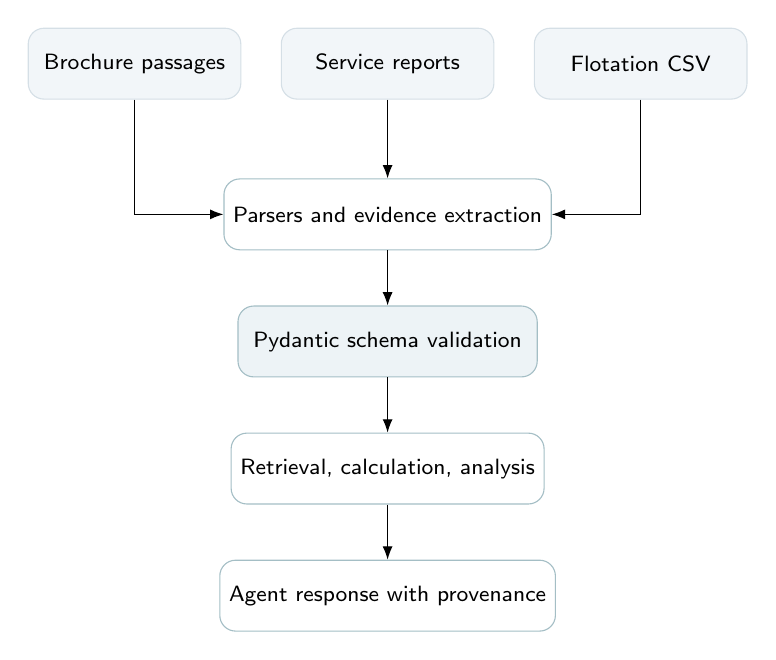
\begin{tikzpicture}[node distance=6mm,>=Latex,
  every node/.style={font=\sffamily\footnotesize,align=center},
  source/.style={draw=Rule,fill=Pale,rounded corners=2mm,minimum width=2.7cm,minimum height=9mm},
  stage/.style={draw=Sea!50,fill=white,rounded corners=2mm,minimum width=3.8cm,minimum height=9mm}]
\node[source] (b) {Brochure passages};
\node[source,right=5mm of b] (s) {Service reports};
\node[source,right=5mm of s] (f) {Flotation CSV};
\node[stage,below=10mm of s] (p) {Parsers and evidence extraction};
\node[stage,below=7mm of p,fill=Blue!8] (v) {Pydantic schema validation};
\node[stage,below=7mm of v] (t) {Retrieval, calculation, analysis};
\node[stage,below=7mm of t] (a) {Agent response with provenance};
\draw[->] (b.south) |- (p.west); \draw[->] (s.south) -- (p.north); \draw[->] (f.south) |- (p.east);
\draw[->] (p)--(v); \draw[->] (v)--(t); \draw[->] (t)--(a);
\end{tikzpicture}
\end{center}
\textbf{The role of Pydantic is specific.} It can reject malformed fields, negative quantities, invalid source-kind combinations and inconsistent identifiers. It cannot, by itself, prove that a cited brochure claim is true, that a reported hour is billable, that a product fits a particular customer installation, or that a current Chilean service quote follows from a historical Swedish report. Those are later extraction, evidence and business-rule responsibilities.

\subsection{Data-contract inventory and exact responsibilities}
\begin{longtable}{@{}L{35mm}L{48mm}L{62mm}@{}}
\toprule\textbf{Class / enum} & \textbf{Important fields} & \textbf{Invariant and downstream use}\\\midrule\endfirsthead
\toprule\textbf{Class / enum} & \textbf{Important fields} & \textbf{Invariant and downstream use}\\\midrule\endhead
\code{EvidenceStatus} & \code{SUPPORTED}, \code{PARTIAL}, \code{INSUFFICIENT}, \code{CONFLICTING} & Expresses evidence completeness and conflicts; not a probabilistic accuracy score.\\
\code{SourceRef} & \code{source_kind}, \code{document_id}, optional \code{page_number}, \code{location} & Carries the identifier needed to trace a tool output back to its input domain.\\
\code{ProductEvidence} & \code{product_name}, \code{chunk_id}, \code{excerpt}, \code{source}, \code{quality_flags} & Requires a brochure source and a positive page reference; feeds product recommendations.\\
\code{CostItem} & \code{category}, \code{description}, \code{quantity}, \code{unit}, \code{unit_rate}, \code{currency}, \code{amount_reported}, \code{source} & Models one historical cost component; derived arithmetic remains separate from reported amount.\\
\code{ServiceReport} & \code{report_id}, visit and site fields, \code{equipment_model}, \code{tasks}, labor/travel hours, cost items, reported total & Preserves a historical visit as a structured record; report source ID must match.\\
\code{FlotationStatistic} & \code{metric}, \code{value}, \code{sample_size}, \code{unit}, \code{source} & Statistical output identifies CSV provenance and a positive sample count.\\
\code{AgentResponse} & \code{answer}, \code{routes}, \code{status}, \code{sources}, \code{warnings}, \code{clarification_question} & Final response structure; a fully supported domain answer must carry a source reference.\\
\bottomrule
\end{longtable}

\subsubsection{SourceRef --- the unit of traceability}
The source identity is constrained to three domains: \code{brochure}, \code{service_report}, and \code{flotation}. A \code{document_id} cannot be blank; a supplied \code{page_number} must be at least one. This enables later audit checks such as verifying that page 2 of a brochure is an actual returned passage. It also lets cost records reject citations to irrelevant brochure sources.

\subsubsection{ProductEvidence --- brochure-grounded technical statements}
A product evidence entry includes its product name, a nonempty passage ID, its text excerpt, a nested source reference and quality flags. The current validator requires the source kind to be \code{brochure} and a positive page number to be present. This is valuable because an answer about Larox or Filter Optimizer must ultimately point to a real brochure passage, not an unstructured recollection of a model response.

\begin{warnbox}
\textbf{Boundary: source location is not semantic proof.} An existing file and page can still be irrelevant to the generated claim. Stage 07 must later verify \emph{claim-to-passage support}, not only that the cited identifier exists.
\end{warnbox}

\subsubsection{CostItem --- observed values and computed amounts}
The cost item model distinguishes \code{amount_reported} from the method \code{derived_amount()}. Its quantity must be greater than zero when present; a unit rate and reported amount must be nonnegative. A source must identify a service report. The three-letter uppercase currency rule validates formatting, not full ISO currency membership or an exchange rate.

For example, a \emph{synthetic} test item with quantity 3, unit rate 12.50 and currency EUR yields \code{Decimal('37.50')}. The corresponding business logic is:
\[
 C_{\mathrm{derived}} = q\times r
 \quad\text{only if }q,\ r\text{ and currency are known.}
\]
If the rate or the currency is unavailable, the current method returns \code{None}. This avoids an especially hazardous error in the Metso case: treating an unpriced service report as a zero-cost service.

\begin{Verbatim}[fontsize=\footnotesize]
from decimal import Decimal

# Synthetic example only: no Metso pricing or report content.
quantity = Decimal("3")
unit_rate = Decimal("12.50")
derived_amount = quantity * unit_rate
assert derived_amount == Decimal("37.50")
\end{Verbatim}

\subsubsection{ServiceReport --- heterogeneous technician visits}
A service record preserves the document identifier \code{FSR-NNNN}, date, country, site, equipment name, activity descriptions, on-site and travel hours, monetary entries, optional total and quality flags. Its model validator requires \code{source.document_id} to equal \code{report_id}, so an apparently valid report cannot silently claim an unrelated source ID.

Not all reports contain a quoted price; consequently \code{reported_total=None} and \code{cost_items=[]} are legitimate structural states. They indicate incomplete monetary evidence, \emph{not} a completed visit with zero cost. Once Stage 04 parses real files, records such as FSR-0027 will need explicit quality flags for truncation and reported-versus-timeline hour disagreements.

\subsubsection{FlotationStatistic --- computed evidence with sample support}
An optional flotation statistic stores a metric name, numeric value, positive sample size, optional unit and a source reference of kind \code{flotation}. In Stage 08 the program must compute each statistic from the CSV, identify the relevant sample and avoid hard-coding the answer to the employer's example. The present model validates the output shape but does not yet calculate a single real plant statistic.

\subsubsection{AgentResponse and EvidenceStatus --- an auditable answer envelope}
\code{AgentResponse} separates the natural-language answer from selected routes, evidence status, source references, warnings and a possible follow-up. A route may be \code{product}, \code{service_cost}, or \code{flotation}. A \code{SUPPORTED} answer with an active domain route requires at least one source. A \code{PARTIAL} answer can honestly identify a missing price and ask who supplies the replacement parts.

\begin{tabularx}{\textwidth}{@{}L{26mm}Y@{}}
\toprule\textbf{Status} & \textbf{Practical use}\\\midrule
\code{SUPPORTED} & Sufficient documented evidence for the particular claim; still no implied commercial guarantee.\\
\code{PARTIAL} & Some relevant evidence exists, but key assumptions, costs or requirements remain unknown.\\
\code{INSUFFICIENT} & The authorized data do not support a defensible answer to the requested question.\\
\code{CONFLICTING} & Available source values disagree materially and the conflict must be surfaced.\\
\bottomrule
\end{tabularx}

\subsection{The thirteen schema tests: exactly what each result establishes}
The supplied targeted Pytest transcript lists every test below as \code{PASSED}. These tests use synthetic values, not employer data, which is appropriate for a public-safe core-validation suite.

\begin{longtable}{@{}L{58mm}L{86mm}@{}}
\toprule\textbf{Test name (abbreviated namespace)} & \textbf{Behavior verified}\\\midrule\endfirsthead
\toprule\textbf{Test name} & \textbf{Behavior verified}\\\midrule\endhead
\path{test_product_evidence_has_page} & A product evidence entry with a brochure source and valid page is accepted.\\
\path{test_product_evidence_missing_page_rejected} & A product evidence entry lacking the required page is rejected.\\
\path{test_cost_item_calculates_derived_amount} & The quantity--rate multiplication yields the exact expected Decimal amount.\\
\path{test_missing_rate_is_not_zero} & The absence of a rate results in \code{None}, not a manufactured zero value.\\
\path{test_unknown_currency_prevents_derived_amount} & Unknown currency prevents the derived monetary amount from being returned.\\
\path{test_negative_quantity_rejected} & A cost item with negative quantity fails Pydantic validation.\\
\path{test_bad_currency_rejected} & An invalid currency string such as \code{euros} is rejected.\\
\path{test_report_can_have_unknown_cost} & A historical report can validly have no reported total and no cost items.\\
\path{test_report_id_mismatch_rejected} & The report ID cannot disagree with the ID of its cited service-report source.\\
\path{test_supported_answer_requires_evidence} & A supported domain answer without any source is rejected.\\
\path{test_partial_answer_can_ask_question} & A partial response may retain a meaningful clarification question.\\
\path{test_flotation_statistic_has_source_and_sample_size} & A valid statistic includes flotation provenance and positive sample size.\\
\path{test_flotation_statistic_rejects_wrong_source} & A flotation statistic cannot cite a service-report source as its provenance.\\
\bottomrule
\end{longtable}

\textbf{Interpretation.} These are \emph{unit tests for the present implementation}, not a benchmark of the full assistant's reasoning quality. They do not yet verify TF--IDF retrieval, extraction of 50 FSRs, Chile-specific prices, meaningful cross-currency aggregation, or citations in generated LLM prose.

\subsection{Exact verified local test transcript and acceptance evidence}
The final targeted and full-suite summaries supplied by the developer were:
\begin{Verbatim}[fontsize=\footnotesize]
# Targeted schema tests
.\.venv\Scripts\python.exe -m pytest tests/test_schemas.py -v
collected 13 items
========================== 13 passed in 0.53s ==========================

# All currently discovered tests
.\.venv\Scripts\python.exe -m pytest -v
collected 14 items
========================== 14 passed in 0.38s ==========================

# Source reference object check
.\.venv\Scripts\python.exe -c "from metso_agent.schemas import
 SourceRef; print(SourceRef(source_kind='brochure',
 document_id='demo', page_number=1).model_dump())"
{'source_kind': 'brochure', 'document_id': 'demo',
 'page_number': 1, 'location': None}
\end{Verbatim}
\textbf{Why the total is fourteen.} Thirteen tests belong to the new \code{test_schemas.py}; one older smoke test checks that the CLI entry-point function is callable. No duplicate schema tests are implied. The two timings reflect separate local test sessions, not a claim about runtime cost of a real AI query.

\subsection{Important limitations discovered by comparing plan and implementation}
A high-quality engineering report should identify gaps \emph{even when all existing tests pass}. The initial design chapters specify a stronger future contract than the small Stage 02 implementation currently proves.

\begin{longtable}{@{}L{39mm}L{55mm}L{50mm}@{}}
\toprule\textbf{Planned requirement} & \textbf{Current evidence} & \textbf{Required follow-up}\\\midrule\endfirsthead
\toprule\textbf{Planned requirement} & \textbf{Current evidence} & \textbf{Required follow-up}\\\midrule\endhead
Origin and page tracking & \code{SourceRef} stores kind, ID and optional page; product evidence requires brochure/page. & Add exact source file path, chunk offsets/section and check genuine claim support later.\\
Product family metadata & Product evidence currently stores \code{product_name}, excerpt, chunk ID. & Add \code{product_family} and extraction method if corpus metadata requires them.\\
Service-part quantities & Report tasks and cost items exist; a complete structured activity/part list is not yet demonstrated. & Extend after Stage 01/04 to capture completed quantities and part-unit ambiguity.\\
Observed versus derived fields & \code{amount_reported} and \code{derived_amount()} are distinct. & Add provenance labels for each extracted rate and compare printed totals against computed totals.\\
Tax and billed-time treatment & Basic reported total, cost items and hours exist. & Add tax treatment, billable-hour basis, date/locale quality flags and source spans.\\
Currency-safe aggregation & Individual currency formatting and unknown-currency behavior are tested. & Implement an aggregator that \emph{rejects mixed-currency sums}; add corresponding tests in Stage 05.\\
Tool output schema & \code{AgentResponse} defined. & Define \code{ToolResult} or typed per-tool return structures during integration.\\
Source validation & Valid domain ID and required page/source kind tested. & Validate actual returned snippets, page indexes and support for generated claims in Stage 07.\\
Real corpus coverage & No raw-file parser, index or inventory results in final output. & Run Stage 01 audit; later integrate actual brochure/FSR/CSV loaders.\\
Design documentation & Code and tests are demonstrated. & Confirm or create \code{docs/data_schema_design.md}.\\
\bottomrule
\end{longtable}

\begin{warnbox}
\textbf{Do not overstate completion.} The fact that all 14 current tests pass proves the named tests pass. It does \emph{not} prove that negative money cannot ever appear downstream, that currencies cannot be mixed by an as-yet-unwritten aggregator, or that a referenced page supports an LLM claim. These are deliberate future engineering gates.
\end{warnbox}

\subsection{Planned integration with actual Metso evidence}
\textbf{Product workflow.} A Markdown brochure loader will read authorized local files, preserve page markers, generate passage IDs, and instantiate \code{ProductEvidence}. Retrieval should return both relevant passages and provenance. For the mandatory changing-feed prompt, Filter Optimizer is a candidate to retrieve, but the evidence object must precede the recommendation; no runtime answer should be hard-coded to the demonstration text.

\textbf{Service workflow.} A parser will convert each report to \code{ServiceReport} and its charges to \code{CostItem}; missing prices remain \code{None}. Stage 04 will classify truncated, bundled and incomplete records. Stage 05 will perform deterministic cost arithmetic with currency integrity. For the Chile request, FSR-0027 is relevant as a historical Swedish 12-cloth task analog; the schema itself must never relabel its reconstructed EUR amount as a confirmed Chile price.

\textbf{Flotation workflow.} When implemented, numeric calculations on \code{flotation_process_data_hourly.csv} will return \code{FlotationStatistic} objects tied to the CSV source and the actual sample count. The schema does not impose contractual concentrate-quality limits, since the supplied dataset does not establish them.

\textbf{Agent workflow.} The controller will choose the correct tool(s), consume validated objects, and produce an \code{AgentResponse} that separates answer prose from source references, warnings and clarifying questions. Source-domain checks must occur before synthesis; LLM-generated wording is not permitted to upgrade a partial or conflicting result into a fully supported commercial claim.

\subsection{Security, reproducibility and source-of-truth boundaries}
The developer's latest Git output showed ignored \code{raw/}, \code{.venv/} and test caches after relocating previously exposed untracked private files. That is an appropriate intermediate control. The final publish gate still requires \code{git ls-files}, inspection of \code{git status}, checking for keys and private copied evidence in README/tests, and reviewing any existing commits. Ignore rules protect \emph{untracked} files; they do not erase a file already committed.

The synthetic test fixtures are intentionally safe to include in a public code-only repository. Real report content, customer names or charges copied from Metso source files should remain under ignored private directories. Because the invitation is marked \term{RESTRICTED}, any use of a third-party model API should also follow the developer's authorized handling of the documents.

\subsection{Recommended final documentation and repeatable verification}
To finish the documentation portion of Stage 02, confirm \code{docs/data_schema_design.md} exists and describes each model, provenance design, validation rules, missing-value handling, current limitations and next consumers. Keep illustrative examples synthetic. Then run:
\begin{Verbatim}[fontsize=\footnotesize]
# From interview/project, in Windows PowerShell
.\.venv\Scripts\python.exe -m pytest tests/test_schemas.py -v
.\.venv\Scripts\python.exe -m pytest -v
.\.venv\Scripts\python.exe -m pip check

# Privacy check before staging or publishing
git check-ignore -v raw/candidate-brief.md
git status --short --ignored
git ls-files

# Check the documentation artifact (not yet evidenced)
Test-Path .\docs\data_schema_design.md
\end{Verbatim}
The test counts should be reported from a fresh run; future additional tests will naturally change the total. The documentation check must only be marked confirmed when its command returns \code{True}. If \code{git ls-files} reveals restricted content, correct the tracking or history before any public push.

\subsection{Stage 02 verification matrix and sign-off judgment}
\begin{tabularx}{\textwidth}{@{}L{10mm}L{101mm}Y@{}}
\toprule\textbf{ID} & \textbf{Acceptance observation} & \textbf{Status}\\\midrule
S02-01 & Python 3.12.4 and Pydantic 2.14.1 are available in \code{.venv}. & Confirmed\\
S02-02 & Git repository initialized; \code{raw/} is ignored. & Confirmed\\
S02-03 & \code{schemas.py} is importable and the schema tests collect. & Confirmed\\
S02-04 & All 13 targeted schema tests pass. & Confirmed\\
S02-05 & All 14 available project tests pass together. & Confirmed\\
S02-06 & A valid \code{SourceRef} can be instantiated and serialized. & Confirmed\\
S02-07 & Public-safe documentation file is present and reviewed. & Not yet shown\\
S02-08 & Full Stage 01 audit outputs and issues exist. & Not yet shown\\
S02-09 & Mixed-currency aggregation fails safely. & Future Stage 05\\
S02-10 & Tool-level and semantic citation checks pass with real evidence. & Future Stages 03--07\\
S02-11 & Tracked files and Git history are verified private-data-free. & Final check pending\\
\bottomrule
\end{tabularx}

\begin{keybox}
\textbf{Engineering sign-off for this chapter.} Stage 02's \emph{core schema implementation and its current unit-test suite are verified}: 13 targeted tests and 14 total tests pass, and direct source-reference serialization succeeds. The broader intended data-contract design is \emph{not fully closed}: the public-safe design memo has not been confirmed, full Stage 01 audit is outstanding, and more sophisticated financial, source-span and citation semantics belong to subsequent implementation stages. The correct next action is to confirm the remaining documentation and complete the real data audit before using these schemas to power product retrieval or cost estimation.
\end{keybox}

\subsection{What this step taught me and how it improves the agent}
This step established the difference between writing plausible text and constructing auditable data. A reference must identify a permitted source. Missing prices must remain unknown. Financial values have both original-document and computed representations. A report identifier must match its purported origin. A final response should declare whether its supporting evidence is sufficient, partial, missing or conflicting. The sequence also demonstrated disciplined debugging: the first import failure was a missing file, not a reason to reinstall Python, and the repair was proven by tests instead of assumed from an editor view.

The most valuable outcome is a stable foundation for the next engineering work. These contracts will allow independent modules to exchange structured evidence and will create points where unsupported claims, invalid numbers or source mismatches can be detected before they reach a salesperson. The full-quality objective remains to verify these contracts against real source files, build and evaluate the mandatory tools, and deliver a small, explainable, evidence-grounded agent within the submission requirements.

\vspace{4mm}
\begin{center}
{\sffamily\color{Gray}\footnotesize END OF PART V -- STAGE 02 TYPED DATA CONTRACTS AND EVIDENCE PROVENANCE}\\[2mm]
{\sffamily\bfseries\color{Navy}AG is your G!}
\end{center}

\clearpage
\section{Step Three --- Stage 03: Brochure-Grounded Product Retrieval}
\begin{center}
{\sffamily\large\bfseries\color{Blue}3.5 Stage 03 --- Build and test brochure-grounded product retrieval}\\[2mm]
{\sffamily\color{Gray}\small Implementation record, technical rationale, observed results, and honest completion gate}
\end{center}

\begin{keybox}
\textbf{Purpose and scope.} This sixth chapter documents how I developed the independent product-retrieval component for the Metso Sales Assistant Agent. It explains each Stage 03 action, why it was necessary, what the code produces, the tests performed, and the evidence and limitations visible at the time of the report. It expands the \emph{planned} Stage 03 in Section 3.5 into a concrete implementation account. No previous chapter is replaced.

\textbf{Verified or previously reported outcome.} Twelve Markdown/PDF brochure pairs were available locally; the retrieval run reported \textbf{89 indexed passages from 12 brochures}; the required Larox changing-feed query returned \code{filter-optimizer.md}, page 2, as its top-ranked hit; \textbf{seven Stage 03 tests and 21 whole-project tests passed} in the user's earlier local verification. The complete runtime repository is not supplied with this report, so these are documented local observations rather than a fresh independent rerun of the Windows project.
\end{keybox}

\subsection{The business requirement and why a retrieval layer comes first}
A salesperson should be able to describe a customer's problem in natural language rather than search a catalog by exact part number. For example, the required prompt describes worsening Larox pressure-filter performance whenever the incoming feed grade changes. A useful system must find \emph{why} a documented product might be relevant rather than simply select the brochure containing the most occurrences of ``Larox.''

The authoritative source for product capabilities and specifications is the \textbf{supplied brochure corpus only}. The 50 historical service reports belong to the separate cost-evidence workflow and must not be treated as technical specifications. The optional flotation CSV belongs to a third evidence domain. Stage 03 therefore implements a narrowly defined tool: it receives a query and returns ranked, traceable \emph{evidence candidates}, not a commercial proposal, diagnosis, or completed conversational answer.

\textbf{Architecture decision.} I deliberately built the lexical retrieval baseline \emph{before} adding an LLM controller. A deterministic local search tool is inexpensive to run, easier to debug, and independently testable. It also creates a precise boundary: the future agent may choose and explain retrieved claims, but it should not create undocumented product specifications.

\subsection{03.1 --- Prerequisites, repository location, and baseline checks}
The development environment is Windows 64-bit with \textbf{Python 3.12.4} inside \code{.venv}. For Stage 03, \code{scikit-learn 1.9.1} was shown installed in the VS Code terminal. Earlier Stage 02 verification had established an importable Pydantic schema module, one CLI smoke test, and 13 passing schema tests. The project is the existing \code{interview/project} directory, \emph{not} an additional nested repository.

\begin{Verbatim}[fontsize=\footnotesize]
# Run in the existing interview/project directory (PowerShell)
.\.venv\Scripts\python.exe --version
.\.venv\Scripts\python.exe -m pip show scikit-learn
.\.venv\Scripts\python.exe -m pytest -q
(Get-ChildItem '.\raw\data\brochures' -Filter '*.md').Count
(Get-ChildItem '.\raw\data\brochures' -Filter '*.pdf').Count
Test-Path '.\src\metso_agent\schemas.py'
\end{Verbatim}

\textbf{Why these checks mattered.} The search module depends on an isolated Python interpreter, a valid TF--IDF implementation, and the \code{ProductEvidence}/\code{SourceRef} contracts from Stage 02. Missing or misplaced source files would invalidate the demonstration before any ranking could be evaluated. The reported inventory of 12 Markdown and 12 PDF files does not, by itself, certify the PDF content; paired-stem and page-marker validation is handled in the loader.

\begin{tabularx}{\textwidth}{@{}L{45mm}L{48mm}Y@{}}
\toprule
\textbf{Dependency} & \textbf{Observed / expected} & \textbf{Role}\\
\midrule
Python interpreter & 3.12.4 (observed) & Runs parsing, search, and tests.\\
\code{scikit-learn} & 1.9.1 (observed) & Builds sparse TF--IDF vectors.\\
\code{schemas.py} & Present and importable in Stage 02 & Validates evidence metadata.\\
Brochure pairs & 12 Markdown and 12 PDF files & Sole product-knowledge corpus.\\
Previous suite & 14 passing tests before Stage 03 & Regression baseline.\\
\bottomrule
\end{tabularx}

\subsection{03.2 --- Create a focused retrieval package}
Rather than mixing document loading, ranking, CLI routing and service-cost logic, I placed product retrieval in a small Python subpackage. The actual implementation uses \code{retrieval/brochure_loader.py} and \code{retrieval/product_search.py}, names that differ harmlessly from some illustrative file names in the early architectural plan.

\begin{Verbatim}[fontsize=\footnotesize]
project/
  raw/                          # restricted employer data
    data/brochures/             # 12 Markdown/PDF brochure pairs
  src/metso_agent/
    __init__.py
    cli.py                      # existing development CLI
    schemas.py                  # Stage 02 typed evidence
    retrieval/
      __init__.py
      brochure_loader.py        # pages, chunks, provenance
      product_search.py         # TF-IDF index, ranking, local CLI
  tests/
    test_smoke.py
    test_schemas.py
    test_product_retrieval.py
  docs/product_retrieval.md     # sanitized design description
\end{Verbatim}

\textbf{Why modularity matters.} This layout allows unit tests to instantiate a loader or index without calling an API. It makes it clear where to fix a source-extraction defect versus a ranking defect, and will later let an agent controller invoke \code{ProductSearcher.search()} through a stable tool interface. It avoids unnecessary model frameworks for a 12-document corpus.

\subsection{03.3 --- Implement the brochure loader and preserve source identity}
\subsubsection{Read each Markdown/PDF pair from the authorized directory}
The loader reads local UTF-8-with-optional-BOM text and compares the stems of all \code{*.md} files with all \code{*.pdf} files. It fails when a Markdown or PDF partner is missing. The PDF is retained as the visual authority for ambiguous tables and specifications; the current runtime \emph{does not extract or validate the PDF text itself}.

\subsubsection{Use explicit page headings as citation boundaries}
The page parser detects headings such as \code{#### Page 2}. It checks that page numbers are consecutive from one, rejecting absent, duplicate, unordered, or skipped page markers. This is deliberately strict: an invalid page map must not silently produce persuasive but fictitious citations.

A useful simplified view of the underlying algorithm is:
\begin{Verbatim}[fontsize=\footnotesize]
for md_file in brochure_files:
    assert matching_pdf_exists(md_file)
    pages = split_at_explicit_page_markers(md_file)
    assert page_numbers_are_consecutive(pages)
    for page_number, page_text in pages:
        for window in page_local_overlapping_windows(page_text):
            emit ProductEvidence(
                excerpt=window.text,
                chunk_id=stable_document_page_window_id,
                source=SourceRef(
                    source_kind='brochure',
                    document_id=md_file.stem,
                    page_number=page_number,
                    location=window.local_offsets,
                ),
            )
\end{Verbatim}

This is an explanatory pseudocode outline, not a copy of the restricted documents. Actual source strings remain in the user's ignored \code{raw/} folder.

\subsubsection{Chunk one page at a time: 300 words with 45-word overlap}
The implemented settings are \textbf{300 whitespace-delimited words per window} and \textbf{45 overlapping words}, producing an effective stride of \(300-45=255\) words. A short page becomes one chunk; a longer page becomes multiple chunks. Because the outer loop processes one page at a time, a passage never crosses a citation page boundary.

\begin{center}
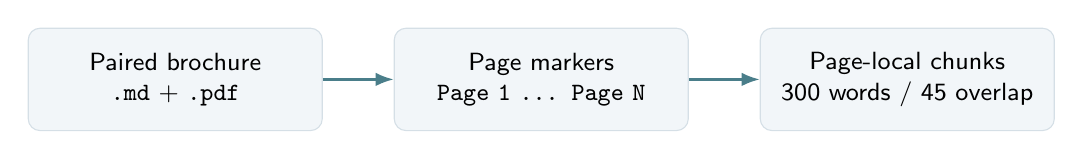
\begin{tikzpicture}[node distance=5mm,>=Latex,
  unit/.style={draw=Rule,fill=Pale,rounded corners=1.5mm,text width=35mm,align=center,minimum height=13mm,font=\sffamily\small},
  arrow/.style={-{Latex[length=2.3mm]},thick,color=Sea}]
\node[unit] (doc) {Paired brochure\\\code{.md} + \code{.pdf}};
\node[unit,right=9mm of doc] (pages) {Page markers\\\code{Page 1 ... Page N}};
\node[unit,right=9mm of pages] (chunks) {Page-local chunks\\300 words / 45 overlap};
\draw[arrow] (doc)--(pages);
\draw[arrow] (pages)--(chunks);
\end{tikzpicture}
\end{center}

\textbf{Why this choice.} It is a simple, measurable baseline. Overlap reduces the risk of cutting a useful statement at a window boundary. Page-local splitting preserves meaningful source references. The initial plan mentioned 350--650 \emph{tokens} and optional semantic/heading-aware segmentation; the actual implementation uses \emph{words} and character positions, and is not claimed to provide heading-aware or table-preserving chunking. These are explicitly recognized future improvements rather than capabilities silently attributed to the current code.

\subsubsection{Attach typed provenance to every chunk}
Each emitted passage is an instance of the Stage 02 \code{ProductEvidence} model. Its associated \code{SourceRef} contains the document stem, the source kind \code{brochure}, the page number, and a page-local span such as \code{page_char:...}. The chunk ID is stable for a fixed source and splitting configuration, for example \code{filter-optimizer:p2:c01}. This permits downstream traceability and regression testing.

\begin{warnbox}
\textbf{Precise provenance limitation.} The recorded character span identifies positions in the loader's \emph{trimmed page text}, not an independently verified absolute byte range in the original Markdown or PDF. A ``page exists'' check is weaker than checking whether a particular technical claim is \emph{entailed} by the cited passage. The latter belongs to Stage 07.
\end{warnbox}

\subsection{03.4 --- Build the lexical baseline with two TF--IDF views}
The search module uses \code{TfidfVectorizer} from scikit-learn. The first vectorizer represents word unigrams and bigrams, lowercases text, removes English stopwords and applies sublinear term frequency. The second vectorizer captures character \(n\)-grams of lengths 3--5 using \code{char_wb}. Character-level matching helps with variations in spelling or minor word-form differences, while word-level matching captures exact equipment names and technical phrases.

For each customer query \(q\) and brochure chunk \(d\), the implemented combined ranking score is
\[
S(q,d)=0.75\,S_{\mathrm{word}}(q,d)+0.25\,S_{\mathrm{character}}(q,d).
\]
The two component scores arise from normalized sparse-vector dot products (cosine-like TF--IDF similarity). \textbf{A score is a ranking signal, not a probability that a recommendation is true.} The coefficients 0.75 and 0.25 are initial engineering settings, not learned, calibrated or globally optimal weights.

\textbf{Query-time behavior.} The function \code{expand_query()} adds task-related search vocabulary when a query contains concepts involving filtration, changing operating conditions, performance or filter cloths. This addresses possible differences between ordinary customer wording and brochure terminology. Expansion is not a license to assume new process measurements or source facts. In particular, \emph{feed grade change} is not automatically evidence of a particular slurry density, particle-size shift or moisture change.

\textbf{Bounded selection.} The default search returns up to five results and at most two chunks per document. Non-positive scores are suppressed; empty queries and invalid count limits produce clear errors. A deterministic tie-break on the chunk ID makes repeated rankings easier to reproduce. Showing only a few passages avoids overwhelming the future agent with duplicates of one long brochure.

\begin{tabularx}{\textwidth}{@{}L{45mm}L{43mm}Y@{}}
\toprule\textbf{Setting} & \textbf{Implemented value} & \textbf{Reason and qualification}\\\midrule
Word TF--IDF & 1--2 word terms & Exact technical word/phrase matching.\\
Character TF--IDF & 3--5 character \(n\)-grams & Tolerates local wording variation.\\
Combination weights & 0.75 word / 0.25 character & Transparent baseline, not calibrated.\\
Query expansion & Small rule-based dictionary & Bridges vocabulary; does not establish facts.\\
\code{top_k} & 5 by default & Returns a focused evidence set.\\
\code{max_per_document} & 2 by default & Prevents one brochure dominating the result list.\\
No-match behavior & No positive lexical match & No invented product answer.\\
\bottomrule
\end{tabularx}

\subsection{The end-to-end Stage 03 data path}
\begin{center}
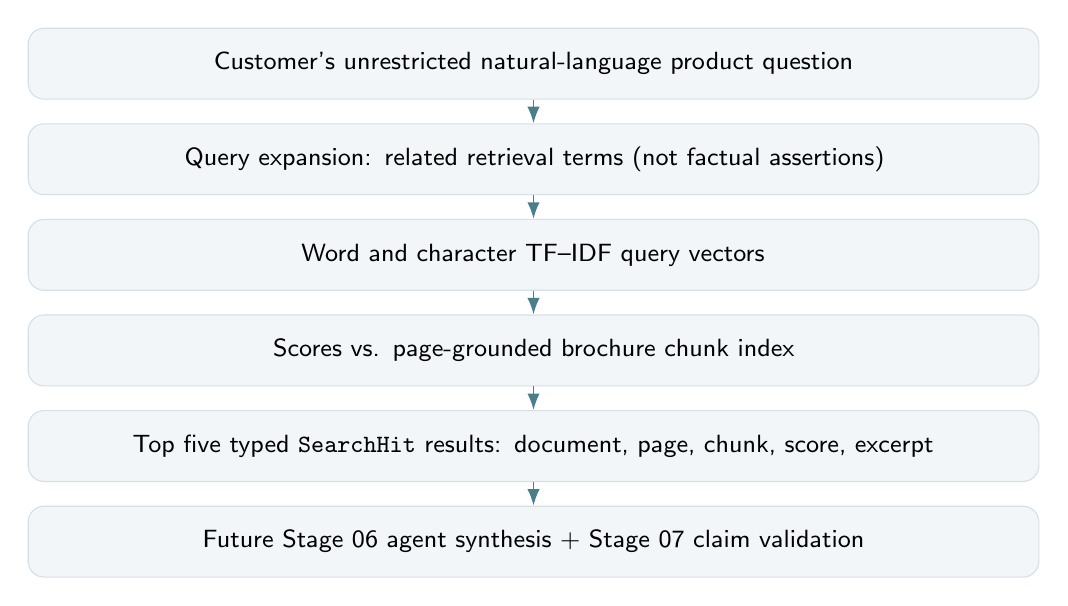
\begin{tikzpicture}[>=Latex,node distance=3mm,
 stage/.style={draw=Rule,fill=Pale,rounded corners=2mm,align=center,text width=126mm,minimum height=9mm,font=\sffamily\small},
 next/.style={-{Latex[length=2.1mm]},line width=0.65pt,draw=Sea}]
\node[stage] (q) {Customer's unrestricted natural-language product question};
\node[stage,below=of q] (exp) {Query expansion: related retrieval terms (not factual assertions)};
\node[stage,below=of exp] (vec) {Word and character TF--IDF query vectors};
\node[stage,below=of vec] (rank) {Scores vs. page-grounded brochure chunk index};
\node[stage,below=of rank] (out) {Top five typed \code{SearchHit} results: document, page, chunk, score, excerpt};
\node[stage,below=of out] (future) {Future Stage 06 agent synthesis + Stage 07 claim validation};
\foreach \a/\b in {q/exp,exp/vec,vec/rank,rank/out,out/future}{\draw[next](\a)--(\b);}
\end{tikzpicture}
\end{center}
The upper five boxes are the implemented retrieval path. The final box represents later integration; it is \emph{not} a capability verified by the Stage 03 tests.

\subsection{03.5 --- Run the mandatory Larox product scenario}
\textbf{Employer-provided demonstration query:}
\begin{examplebox}
\emph{We have Larox pressure filters but performance drops whenever our feed grade changes}
\end{examplebox}
The command-line runner loads the local corpus, builds the TF--IDF index and ranks the question. It prints a compact source/page/score summary and a short excerpt preview. The developer can inspect source identity without making a complete agent call.

\begin{Verbatim}[fontsize=\footnotesize]
.\.venv\Scripts\python.exe -m metso_agent.retrieval.product_search `
  'We have Larox pressure filters but performance drops whenever our feed grade changes' `
  --top-k 5
\end{Verbatim}

The earlier local verification reported \textbf{89 chunks indexed from 12 brochures} and the following ranked output. Scores are displayed to three decimal places and should be treated as \emph{observed for that run}, not as permanent thresholds:
\begin{tabularx}{\textwidth}{@{}L{10mm}L{72mm}L{20mm}Y@{}}
\toprule\textbf{Rank} & \textbf{Brochure} & \textbf{Page} & \textbf{Score}\\
\midrule
1 & \code{filter-optimizer.md} & 2 & 0.254\\
2 & \code{larox-pf-ds.md} & 2 & 0.172\\
3 & \code{filter-optimizer.md} & 2 & 0.159\\
4 & \code{larox-pf-brochure-b.md} & 4 & 0.147\\
5 & \code{larox-pf-brochure-a.md} & 2 & 0.145\\
\bottomrule
\end{tabularx}

\textbf{Why the first result is useful.} The Filter Optimizer brochure discusses adjusting filter operation cycle by cycle under changing process characteristics. The documented variables include feed amount, pressing differential pressure and air-drying time. The Larox PF brochures add information about the filtration equipment and variants. Thus the top result supports a plausible \emph{investigation candidate} rather than a mere lexical match to ``Larox.''

\textbf{What it does not establish.} The query does not specify the exact Larox model, the measurement defining ``performance'', which feed characteristic actually changed, or whether a specific optimizer retrofit is compatible. A proper future answer should ask whether throughput, cycle time or residual cake moisture has deteriorated, and should not represent changing \emph{grade} as proof of changing \emph{density}.

\subsection{03.6 --- Try paraphrases, distinct products, and a false guarantee}
One successful employer prompt is insufficient proof of general retrieval quality. The local follow-up tests broadened the surface of the problem to nearby wording, other product families and a deliberately unsupported commercial statement.

\begin{longtable}{@{}L{45mm}L{57mm}L{42mm}@{}}
\toprule\textbf{Probe} & \textbf{Observed first hit} & \textbf{Interpretation}\\
\midrule\endfirsthead
\toprule\textbf{Probe} & \textbf{Observed first hit} & \textbf{Interpretation}\\
\midrule\endhead
Unstable pressure-filter operation when conditions change & \code{filter-optimizer.md}, p. 2; score 0.233 & Relevant capability retrieved using a paraphrase.\\
Question about the Orion series pump & \code{orion-series-pump.md}, p. 1; score 0.586 & Retrieval applies beyond the Larox case.\\
Question about CellStation air/level control & \code{cellstation.md}, p. 1; score 0.156 & Retrieves a separate flotation-control product.\\
Claim of a guaranteed 50\% saving with Larox & \code{larox-pf-ds.md}, p. 2 & A related hit \emph{does not} substantiate the claimed saving.\\
\bottomrule
\end{longtable}

\textbf{Negative-case lesson.} A brochure passage mentioning ``guaranteed'' in a different context (such as cake discharge) is not evidence for a universal \emph{50\% saving}. Lexical retrieval cannot decide that kind of semantic entailment reliably. For the future conversational system, an affirmative guarantee must be blocked unless the specific statement, conditions and scope are actually supported by the cited source. This is a planned Stage 07 claim-support gate, not an existing Stage 03 feature.

\subsection{03.7 --- Add seven independent retrieval unit tests}
The new test module \code{tests/test_product_retrieval.py} uses \textbf{synthetic} Markdown text and dummy PDF pair files. Test fixtures do not reproduce Metso's proprietary brochures, historical prices or customer reports. This permits a useful public code-only test suite while preserving the source-data boundary.

\begin{longtable}{@{}L{58mm}L{84mm}@{}}
\toprule\textbf{Test} & \textbf{What passing establishes}\\
\midrule\endfirsthead
\toprule\textbf{Test} & \textbf{What passing establishes}\\
\midrule\endhead
\code{test_page_provenance} & Distinct source pages retain the correct document ID and page numbers.\\
\code{test_missing_pdf_pair_fails} & A Markdown brochure without its paired PDF triggers a clear failure.\\
\code{test_missing_page_marker_fails} & Unmarked text is not treated as a safely citable page.\\
\code{test_nonconsecutive_pages_fail} & A skipped or discontinuous source page sequence is rejected.\\
\code{test_search_finds_relevant_product} & A synthetic changing-filtration question favors the corresponding filter-optimization description over an unrelated pump description.\\
\code{test_empty_query_rejected} & Blank input fails validation rather than returning a misleading ranking.\\
\code{test_chunks_never_cross_pages} & A multi-window source preserves strict page boundaries.\\
\bottomrule
\end{longtable}

These are seven \emph{behavioral tests}, not seven independent guarantees about all industrial recommendations. For example, the pairing test confirms filenames, not that a valid PDF file can be rendered; and the relevance test examines a small synthetic corpus, not a statistically representative sample of customer questions.

\subsection{03.8 --- Targeted and complete regression results}
The developer's previous session reported the dedicated Stage 03 suite passing all seven cases and the complete project suite passing \textbf{21 tests}: one CLI smoke test, 13 Stage 02 schema tests, and seven Stage 03 retrieval tests. No failures were reported in those sessions.

\begin{Verbatim}[fontsize=\footnotesize]
# Dedicated retrieval checks
.\.venv\Scripts\python.exe -m pytest tests/test_product_retrieval.py -v
# Reported: 7 passed

# Complete local regression suite
.\.venv\Scripts\python.exe -m pytest -v
# Reported: 21 passed
\end{Verbatim}

\begin{tabularx}{\textwidth}{@{}L{73mm}L{35mm}Y@{}}
\toprule\textbf{Test group} & \textbf{Passed / run} & \textbf{Result}\\
\midrule
Stage 02 schema tests & 13 / 13 & Pass (previous stage)\\
Stage 03 retrieval tests & 7 / 7 & Pass\\
Existing CLI smoke test & 1 / 1 & Pass\\
\midrule
\textbf{Total project suite} & \textbf{21 / 21} & \textbf{All passed}\\
\bottomrule
\end{tabularx}

\begin{keybox}
\textbf{Interpretation of the 21/21 result.} It demonstrates that the \emph{defined tests} passed in the reported environment. It does not show a validated retrieval recall@5, a production-ready recommendation engine, a service-cost estimate, autonomous tool routing, or factual correctness of an LLM-generated answer. Those require additional evidence and separate tests.
\end{keybox}

\subsection{03.9 --- Document the implementation and protect restricted data}
The VS Code screenshot confirms that \code{docs/product_retrieval.md} exists and includes its concluding sections about limitations and confidentiality. Its complete content has not been independently inspected line by line through the uploaded materials. The implementation memo should document corpus boundaries, chunking, scoring and search parameters, tests, reproducibility commands, and present limitations without embedding private source excerpts.

The actual brochure files remain under the Git-ignored \code{raw/} directory. A previous Git test confirmed the ignore rule for restricted source material, but the \textbf{final tracked-file and commit-history audit is still pending}. This distinction matters: \code{.gitignore} does not remove a private file already committed. Additionally, the developer's VS Code view showed private five-part PDF/TeX study reports in the repository root; these should be stored in an ignored private location after checking for filename collisions.

\begin{Verbatim}[fontsize=\footnotesize]
# Final local verification, before any publication
Test-Path '.\docs\product_retrieval.md'
Test-Path '.\src\metso_agent\retrieval\brochure_loader.py'
Test-Path '.\src\metso_agent\retrieval\product_search.py'
.\.venv\Scripts\python.exe -m pytest -q
git status --short --ignored
git ls-files
# Inspect tracked files and commit history for any private data.
\end{Verbatim}

\subsection{A closer engineering review: what has and has not been delivered}
\begin{longtable}{@{}L{45mm}L{47mm}L{52mm}@{}}
\toprule\textbf{Area} & \textbf{Established evidence} & \textbf{Remaining work / qualification}\\
\midrule\endfirsthead
\toprule\textbf{Area} & \textbf{Established evidence} & \textbf{Remaining work / qualification}\\
\midrule\endhead
Brochure enumeration & 12 pairs indexed in local run & Full content/page-to-PDF agreement should be audited.\\
Page-grounded chunks & Seven synthetic tests; 89 reported real chunks & Original PDF text/table verification is not implemented.\\
Typed evidence references & Loader emits Stage 02 models with page/ID/span & Claim-level evidence entailment is not yet checked.\\
Lexical ranking & TF--IDF returns relevant Larox, Orion and CellStation top hits & No labeled holdout recall@5 or semantic benchmark yet.\\
Query expansion & Simple rule-based terms available & Requires false-positive analysis and product/model disambiguation.\\
Customer response & Search results and excerpt previews only & No autonomous conversational synthesis or clarification here.\\
Confidentiality & \code{raw/} ignored in earlier Git tests & \code{git ls-files}, history, generated artifacts and public preview pending.\\
Documentation & \code{product_retrieval.md} visible in editor & Full text review and reproducibility check pending.\\
Stage 01 source audit & Count checks and earlier audit methodology & Comprehensive executed audit evidence remains outstanding.\\
\bottomrule
\end{longtable}

\subsection{Why I did not add embeddings or a vector database}
For the current corpus of only 12 brochures, the TF--IDF baseline is interpretable and demonstrated to retrieve the principal product candidates. Building an external vector database or a complicated hybrid search architecture before measuring retrieval failures would increase implementation time, dependency risk and confidentiality surface area. The appropriate next decision is empirical: create a private, labeled set of varied queries, calculate document- and passage-level recall@5 and inspect false matches. Only if the observed failure cases justify the extra complexity should embeddings or reranking be introduced.

An important future error category is short product-name overlap: a PF and a PF-DS are related but not interchangeable. Character-level similarity and query expansion can amplify that confusion. A model/variant disambiguation check should therefore accompany any stronger semantic retrieval.

\subsection{Exact acceptance commands and interpretation guide}
All commands below assume the user's actual \code{interview/project} root and its local virtual environment. They make the stage independently reproducible by an authorized developer who has the original data on disk.

\begin{Verbatim}[fontsize=\footnotesize]
# 1) Confirm the brochure corpus
(Get-ChildItem '.\raw\data\brochures' -Filter '*.md').Count
(Get-ChildItem '.\raw\data\brochures' -Filter '*.pdf').Count

# 2) Verify loader counts and distinct source documents
.\.venv\Scripts\python.exe -c "from pathlib import Path; from metso_agent.retrieval.brochure_loader import load_brochures; a=load_brochures(Path('raw/data/brochures')); print(len(a), len({x.source.document_id for x in a}))"

# 3) Run the exact mandatory product question
.\.venv\Scripts\python.exe -m metso_agent.retrieval.product_search `
  'We have Larox pressure filters but performance drops whenever our feed grade changes' --top-k 5

# 4) Run component and project tests
.\.venv\Scripts\python.exe -m pytest tests/test_product_retrieval.py -v
.\.venv\Scripts\python.exe -m pytest -q

# 5) Inspect Git handling of restricted materials
git check-ignore -v raw/candidate-brief.md
git status --short --ignored
git ls-files
\end{Verbatim}

\textbf{Acceptance interpretation.} The first checks should return 12 and 12. The loader was previously observed to return 89 chunks representing 12 brochures. The mandatory query should show a relevant Filter Optimizer passage with a true page reference, not a fabricated final recommendation. The test suites should remain green. The Git report must reveal no tracked private materials. If any result differs, record the actual behavior and investigate; do not change a benchmark target merely to make the report appear successful.

\subsection{Stage 03 sign-off matrix}
\begin{tabularx}{\textwidth}{@{}L{13mm}L{106mm}Y@{}}
\toprule\textbf{ID} & \textbf{Stage 03 observation or requirement} & \textbf{Status}\\
\midrule
S03-01 & Python, scikit-learn and typed schema dependencies are usable. & Confirmed\\
S03-02 & Twelve brochure pairs are found in the authorized local path. & Confirmed\\
S03-03 & Page-marker validation and page-local chunking pass synthetic tests. & Confirmed\\
S03-04 & Indexed real corpus run reports 89 chunks from 12 brochures. & Reported\\
S03-05 & Required Larox prompt finds Filter Optimizer, page 2, as top hit. & Reported\\
S03-06 & Orion, CellStation and a changing-conditions paraphrase retrieve relevant first hits. & Reported\\
S03-07 & All seven targeted retrieval tests pass. & Confirmed\\
S03-08 & Entire 21-test project suite passes. & Confirmed\\
S03-09 & Sanitized retrieval-design memo exists; full content reviewed. & Partly confirmed\\
S03-10 & Tracked Git files/history inspected for confidential content. & Pending\\
S03-11 & Labeled multi-query recall@5 is measured and satisfactory. & Future Stage 09\\
S03-12 & Generated claims are semantically checked against retrieved passages. & Future Stage 07\\
S03-13 & Autonomous agent selects this tool and delivers a grounded answer. & Future Stage 06\\
\bottomrule
\end{tabularx}

\begin{keybox}
\textbf{Engineering conclusion.} Stage 03's \emph{core local retrieval implementation is successful}: the 12-brochure corpus was indexed, page-grounded evidence was returned for the mandatory Larox query, cross-product probes were run, and the seven dedicated plus 21 total tests passed in the reported Windows sessions. It is not accurate to call the \emph{complete Metso AI agent} finished. The remaining gates are final Git/document review, broader labeled evaluation, semantic claim-support checks, and conversational integration with the separate historical-service workflow.
\end{keybox}

\subsection{What this stage taught me and the hand-off to Stage 04}
This stage converted a static brochure folder into an inspectable, testable evidence service. The most important implementation decision was to preserve \emph{document identity, exact page identity and chunk identity} all the way from ingestion to the search output. This made the retrieval result independently checkable and provided a clean input for the later LLM controller. Pair-validation, strict page-marker checks and synthetic regression tests turned silent evidence corruption into explicit errors.

The main business result is not that a search score reached a certain number. It is that a natural-language complaint about changing Larox filtration performance can discover the documented Filter Optimizer candidate \emph{without claiming unverified retrofit compatibility or guaranteed savings}. The principal engineering lesson is equally important: lexical relevance is not factual support. That gap must be closed deliberately in the answer-validation stage.

The next separate component is \textbf{Stage 04: Historical Service Report Extraction}, where the 50 technician reports will be parsed into typed, quality-flagged records for later cost estimation. Stage 03 retrieval and Stage 04 extraction may be developed independently, but both must be integrated by the Stage 06 controller before the two required demonstrations count as a working agent.

\vspace{4mm}
\begin{center}
{\sffamily\color{Gray}\footnotesize END OF PART VI -- STAGE 03 BROCHURE-GROUNDED PRODUCT RETRIEVAL}\\[2mm]
{\sffamily\bfseries\color{Navy}AG is your G!}
\end{center}


\clearpage
\section{Stage 04 --- Extract and verify the historical service reports}
\label{sec:executed-stage04}
\begin{keybox}
\textbf{Implementation status at 18 October 2026.} The local Stage 04 ingestion pipeline was executed against the \textbf{50 supplied historical field-service reports}. It produced a private structured ledger with 50 records and a separate quality-issue file with \textbf{41 flagged reports}. The developer's Windows terminal shows \textbf{12/12 dedicated parser tests passed} and \textbf{33/33 project tests passed}. The generated records are \emph{provisional evidence}, not fully adjudicated source truth: the human-review worksheet is present, but the visible decisions are still \code{Pending}. Stage 05 pricing must not treat those entries as approved historical rates until material fields have been checked against the originals.
\end{keybox}

\subsection{The question I needed to solve and why this stage matters}
The second mandatory business capability is a rough, defensible budget for a technician visit. A sales agent cannot responsibly estimate a Larox PF-DS cloth replacement simply by searching for a total that looks similar. Historical reports mix completed work, intended work, travel, on-site labor, parts, tax, contract amounts, missing invoices and different currencies. The input is \emph{semi-structured evidence}, not an invoice database.

My Stage 04 objective was therefore narrower than quotation: \textbf{convert the fifty heterogeneous technician files into typed, traceable records without inventing missing values}. The next stage will decide which records are appropriate comparisons and apply deterministic arithmetic. Separating extraction from estimation makes parsing failures detectable before they affect a customer-facing budget.

\begin{tabularx}{\textwidth}{@{}L{33mm}Y Y@{}}
\toprule
\textbf{Layer} & \textbf{Responsibility} & \textbf{Deliberate limitation}\\
\midrule
Original text reports & Provide the only permitted historical service-cost observations. & The files are heterogeneous and sometimes incomplete.\\
Stage 04 parser & Extract typed values, source positions, hashes, and quality indicators. & Does not issue a quote or invent missing monetary details.\\
Private review ledger & Retain recoverable evidence and ambiguous candidates. & Entries with flags require source-level adjudication.\\
Stage 05 estimator & Select comparators and compute well-supported historical breakdowns. & Must not silently substitute a Chile tariff or mix currencies.\\
Agent controller & Choose tools and communicate a qualified answer. & Not demonstrated by Stage 04 tests.\\
\bottomrule
\end{tabularx}

\subsection{04.1 --- Verify the environment, prior regression baseline, and input coverage}
\textbf{What I did.} I worked in the existing Windows project under the \code{interview/project} directory, with its activated Python virtual environment. I verified Python \textbf{3.12.4}, ran the previously established tests, counted the input reports, and checked the typed-schema module. The baseline before installing Stage 04 remained \textbf{21 passed in 4.48 seconds}. The report glob returned exactly \textbf{50} files named \code{FSR-*.txt}, and the Stage 02 \code{schemas.py} file existed.

\textbf{Why.} This made the Stage 04 change attributable to a new component, not an already-broken development environment. It also made explicit that the expected corpus contains 50 visits; a successful extraction from only 49 files would be a coverage failure.

\begin{Verbatim}[fontsize=\footnotesize]
.\.venv\Scripts\python.exe --version
.\.venv\Scripts\python.exe -m pytest -q
(Get-ChildItem '.\raw\data\HistoricalServices' -Filter 'FSR-*.txt').Count
Test-Path '.\src\metso_agent\schemas.py'
\end{Verbatim}

\textbf{Observed output.} Python 3.12.4; \code{21 passed in 4.48s}; report count \code{50}; schema existence \code{True}. One early terminal error arose when a long Windows path containing spaces was typed as if it were an executable command. It did not stop or invalidate the subsequent successful tests. Paths with spaces should instead be handled with \code{Set-Location -LiteralPath} or quoted arguments.

\subsection{04.2 --- Add a dedicated ingestion package without replacing earlier work}
The Stage 04 code was added to the existing project tree, preserving the Stage 02 schemas and Stage 03 brochure retrieval. Four file-existence checks returned \code{True} for the parser, its synthetic tests, the local review script and the extraction-design document.

\begin{Verbatim}[fontsize=\footnotesize]
project/
  raw/data/HistoricalServices/FSR-0001.txt ... FSR-0050.txt  # private
  src/metso_agent/schemas.py                         # Stage 02
  src/metso_agent/retrieval/                          # Stage 03
  src/metso_agent/ingestion/__init__.py               # Stage 04
  src/metso_agent/ingestion/service_parser.py         # Stage 04
  tests/test_service_parser.py                        # Stage 04
  scripts/review_stage04.py                           # Stage 04
  docs/service_extraction.md                          # Stage 04
  docs/private/stage04_gold_review.md                 # private review
  local_cache/service_ledger.json                     # private result
  local_cache/service_quality_issues.json             # private result
\end{Verbatim}

\textbf{Design rationale.} I did not put the parsing logic in the CLI or the LLM controller. The \code{ingestion} package handles extraction; \code{schemas.py} defines accepted shapes; \code{scripts/review_stage04.py} makes inspectable summaries; and \code{tests/test_service_parser.py} exercises edge cases using synthetic material. The reviewer can inspect each responsibility without running a language model.

\subsection{04.3 --- A conservative extraction contract: evidence first, assumptions second}
The parser reads the authorized text files and produces typed service records plus supplementary extraction evidence. The previous Pydantic contracts include report identity, visit date, country/site, equipment model, work descriptions, labor and travel hours, individual cost items, an explicitly reported total, currency and quality flags. The Stage 04 ledger also retains candidate material rows, candidate cost rows, task evidence, source-line locations and source-file hashes where produced.

\begin{tabularx}{\textwidth}{@{}L{39mm}Y@{}}
\toprule
\textbf{Evidence field} & \textbf{Rule used and reason}\\
\midrule
\code{report_id}, source ID & Preserve the FSR identity and support traceable lookup in the original file.\\
\code{visit_date} & Keep unknown or ambiguous date as null; do not infer from geography.\\
Country, site, equipment & Extract when supported; flag ambiguous or unrecognized mentions.\\
Tasks / completed work & Separate performed work from plans, failed attempts and partial completion.\\
Labor and travel hours & Keep source-observed hours separate from clock-time elapsed and travel-direction ambiguity.\\
Itemized monetary rows & Keep individual printed cost-summary amounts and their source locations.\\
Material-row candidates & Retain material mentions separately; do not double-count them with cost-summary rows.\\
\code{reported_total} & Populate only from a complete, printed source total; missing never becomes zero.\\
\code{total_currency} & Do not infer a currency solely from country or an ambiguous dollar symbol.\\
Quality flags / SHA-256 & Explain limitations and permit source-integrity and human-review checks.\\
\bottomrule
\end{tabularx}

\textbf{Crucial distinction.} An itemized monetary row, a materials-list mention and a grand total are three different observations. A materials section can help determine what was installed, but it must not be blindly added to a cost-summary section that already prices the same parts. Similarly, a bundled total cannot safely be decomposed into a unit price without a supporting breakdown.

\subsubsection{The three major source shapes}
\begin{enumerate}
\item \textbf{Itemized report.} Detailed cost-summary rows may permit extraction of hours, quantities, rates, line amounts, tax and total. The parser preserves each cost row's original location rather than silently recalculating an invoice during Stage 04.
\item \textbf{Bundled report.} A reported total may exist while cost rows are absent. The full amount is observed, but the decomposition is unknown; it must never be relabeled a per-cloth price or a labor rate.
\item \textbf{Unpriced, partial or truncated report.} Phrases such as ``invoice to follow'' and ``as per agreement'' are not numeric invoices. Incomplete work must be distinguished from a completed replacement. Truncated tables are retained and flagged rather than completed with guessed values.
\end{enumerate}

\subsubsection{Provenance and reproducibility}
Each record carries source identity, and the source-file SHA-256 makes later changes detectable. Source-line references enable checking a figure in the corresponding private \code{FSR-####.txt} file. A checksum shows that bytes are reproducible; it does \emph{not} independently establish that the parser's interpretation is correct. That requires field-level source review.

\subsection{04.4 --- Test irregular report interpretation before using live files}
I ran the dedicated parser suite before treating any generated ledger as trustworthy. The submitted Windows output collected \textbf{12 tests}, and every one passed in \textbf{0.68 seconds}. The tests intentionally use synthetic report fixtures, so they are suitable for a code-only repository and do not contain verbatim restricted customer reports.

\begin{longtable}{@{}L{68mm}L{77mm}@{}}
\toprule
\textbf{Passed test name} & \textbf{Behavior it checks}\\
\midrule\endfirsthead
\toprule
\textbf{Passed test name} & \textbf{Behavior it checks}\\
\midrule\endhead
{\ttfamily\footnotesize test\_\allowbreak{}itemized\_\allowbreak{}costs\_\allowbreak{}have\_\allowbreak{}lines} & Captures itemized amounts with evidence locations.\\
{\ttfamily\footnotesize test\_\allowbreak{}truncated\_\allowbreak{}does\_\allowbreak{}not\_\allowbreak{}invent\_\allowbreak{}total} & A truncated cost table cannot produce a fabricated printed total.\\
{\ttfamily\footnotesize test\_\allowbreak{}invoice\_\allowbreak{}to\_\allowbreak{}follow\_\allowbreak{}not\_\allowbreak{}zero} & No written price does not mean a zero-charge service.\\
{\ttfamily\footnotesize test\_\allowbreak{}unknown\_\allowbreak{}dollar\_\allowbreak{}does\_\allowbreak{}not\_\allowbreak{}infer\_\allowbreak{}currency} & Ambiguous dollar notation is not assigned a guessed currency.\\
{\ttfamily\footnotesize test\_\allowbreak{}country\_\allowbreak{}not\_\allowbreak{}inferred\_\allowbreak{}from\_\allowbreak{}ambiguous\_\allowbreak{}date} & Ambiguous date interpretation does not establish a country.\\
{\ttfamily\footnotesize test\_\allowbreak{}partial\_\allowbreak{}work\_\allowbreak{}and\_\allowbreak{}travel\_\allowbreak{}each\_\allowbreak{}way\_\allowbreak{}flag} & Partial work and unclear one-way/return travel require flags.\\
{\ttfamily\footnotesize test\_\allowbreak{}report\_\allowbreak{}id\_\allowbreak{}mismatch\_\allowbreak{}flagged} & Conflicting source/report identifiers are detected.\\
{\ttfamily\footnotesize test\_\allowbreak{}wrong\_\allowbreak{}report\_\allowbreak{}count\_\allowbreak{}rejected} & Missing coverage is rejected rather than accepted as a full corpus.\\
{\ttfamily\footnotesize test\_\allowbreak{}no\_\allowbreak{}cross\_\allowbreak{}currency\_\allowbreak{}aggregation} & The tested aggregation path does not silently combine currencies.\\
{\ttfamily\footnotesize test\_\allowbreak{}timeline\_\allowbreak{}is\_\allowbreak{}separate\_\allowbreak{}from\_\allowbreak{}billable\_\allowbreak{}hours} & Clock interval and reported working hours remain distinct.\\
{\ttfamily\footnotesize test\_\allowbreak{}completed\_\allowbreak{}work\_\allowbreak{}and\_\allowbreak{}materials\_\allowbreak{}preserved} & Work-completion and material evidence are retained.\\
{\ttfamily\footnotesize test\_\allowbreak{}bundle\_\allowbreak{}is\_\allowbreak{}not\_\allowbreak{}itemized} & A bundled amount is not misrepresented as line-item detail.\\
\bottomrule
\end{longtable}

\begin{keybox}
\textbf{What 12/12 passing establishes.} The tested extraction decisions worked on the constructed fixtures. It does \emph{not} establish perfect extraction accuracy on all irregular real-world reports, that every field in the 50 resulting records is correct, or that a customer quotation is ready. The private review step exists precisely because synthetic tests cannot cover all document variation.
\end{keybox}

\subsection{04.5 --- Execute the parser on all 50 historical reports}
After the tests passed, I ran the ingestion module against the authorized source directory, writing the structured results into the already-ignored \code{local_cache/} path.

\begin{Verbatim}[fontsize=\footnotesize]
.\.venv\Scripts\python.exe -m metso_agent.ingestion.service_parser `
  --source '.\raw\data\HistoricalServices' `
  --output '.\local_cache\service_ledger.json'
\end{Verbatim}

\textbf{The actual terminal evidence was:}
\begin{Verbatim}[fontsize=\footnotesize]
Processed: 50 reports
Private ledger: local_cache\service_ledger.json
Private issue log: local_cache\service_quality_issues.json
  (41 records flagged)
WARNING: extraction is provisional; review flagged fields
  against originals before pricing.
\end{Verbatim}

Both output-file existence checks returned \code{True}. Reading the ledger as JSON in PowerShell and checking \code{Count} returned \textbf{50}. This verifies that all fifty report IDs are represented in the output collection; it is not proof of the accuracy or completeness of every extracted field.

\subsection{Observed corpus-wide extraction and quality profile}
The following quantities are computed from the \emph{per-report summary lines in the supplied Windows terminal transcript}, rather than assumed from the raw documents. Multiple flags can apply to one report; the category counts below therefore overlap.

\begin{tabularx}{\textwidth}{@{}L{102mm}r@{}}
\toprule
\textbf{Observed measure} & \textbf{Count}\\
\midrule
Source reports processed / ledger records & 50\\
Records with one or more quality flags & 41\\
Records without emitted flags (still eligible for sample review) & 9\\
Reports with at least one parsed cost row & 14\\
Reports with zero parsed cost rows & 36\\
Total parsed cost rows across all reports & 69\\
Reports flagged \code{TASKS_REQUIRE_REVIEW} & 36\\
Reports flagged \code{TOTAL_NOT_REPORTED} & 26\\
Reports flagged \code{EQUIPMENT_REQUIRES_REVIEW} & 23\\
Reports flagged \code{PRICE_NOT_AVAILABLE} & 20\\
Reports flagged \code{BUNDLED_TOTAL_NOT_ITEMIZED} & 12\\
Reports flagged \code{TRUNCATED_COST_TABLE} & 1\\
\bottomrule
\end{tabularx}

\textbf{Interpretation.} Forty-one flags are not forty-one parser crashes. The program deliberately emits review signals where the underlying report is incomplete or interpretation is risky. The nine records with no emitted flags are not automatically ``audited correct'': absence of a detected problem does not prove the parser found everything. Likewise, 36 reports without itemized cost rows may still contain a legitimate bundled total or useful operational information.

The high frequency of task and equipment review flags signals that narrative understanding is a weak point worth prioritizing in a human-reviewed sample. A practical next improvement would be a targeted classifier or additional report-template rules, but only after manually confirming where the current extraction actually fails.

\subsection{04.6 --- Inspect the private artifacts and source-reported values}
Two JSON artifacts were observed in VS Code:
\begin{itemize}
\item \code{local_cache/service_ledger.json}: a list of typed report records with additional observations, candidate cost/material lines, source metadata, flags and hashes.
\item \code{local_cache/service_quality_issues.json}: a compact list of report identifiers and their quality flags; 41 entries were reported during parsing.
\end{itemize}

The user opened both artifacts in VS Code. Their presence and the 50-record count corroborate the CLI's successful output step. Because the outputs contain derived information from restricted reports, they are intentionally local-only and must not be uploaded with public project source code.

For focused verification, I used \code{scripts/review_stage04.py} to display a small set of representative cases. It reads the private ledger without generating a customer quote. Its reported outputs are reproduced below as summaries, with the distinction between \emph{printed totals} and \emph{unpriced evidence} preserved.

\begin{longtable}{@{}L{18mm}L{26mm}L{32mm}L{68mm}@{}}
\toprule
\textbf{ID} & \textbf{Place} & \textbf{Printed total} & \textbf{Observed scope / parsing qualification}\\
\midrule\endfirsthead
\toprule
\textbf{ID} & \textbf{Place} & \textbf{Printed total} & \textbf{Observed scope / parsing qualification}\\
\midrule\endhead
FSR-0027 & Sweden & Missing & PF-DS, 12-cloth case; truncated cost table; 3 parsed rows and 3 material candidates.\\
FSR-0028 & Sweden & Missing & Incomplete intervention; 0 parsed cost rows; equipment and travel need review.\\
FSR-0031 & Finland & EUR 2,580.44 & PF-DS scope including more cloths and hydraulic work; 5 parsed cost rows.\\
FSR-0014 & Canada & CAD 4,367.00 & Broader PF-DS service with additional hydraulic scope; 7 parsed cost rows.\\
FSR-0035 & Chile & USD 2,850 & Filter Optimizer work; bundled total; 0 itemized rows.\\
FSR-0044 & Sweden & SEK 19,850 & PF-DS service with bundled total; 0 itemized rows.\\
\bottomrule
\end{longtable}

\textbf{Why these examples matter.} The six reports cover both close task similarity and distinct geographic context, itemized versus bundled pricing, absent prices, incomplete work, and tax/scope differences. They demonstrate why a simplistic ``take the nearest total'' approach would be unsafe. In particular, no Chilean case shown is a verified exact 12-cloth PF-DS price precedent.

\subsection{04.7 --- The decisive case: FSR-0027 and the 12-cloth PF-DS question}
\begin{warnbox}
\textbf{Source-handling boundary.} The parsed record for \code{FSR-0027} describes a Swedish Larox PF-DS visit at Aitik on 12 May 2023. The local review shows \textbf{8.4 on-site labor hours}, \textbf{4.9 travel hours}, \textbf{three parsed cost-summary rows}, and \textbf{three separate candidate material rows}. Critically, the extracted \code{reported_total} is \code{None}. The parser does not invent the remaining lines of the truncated cost table or silently label an analyst-derived sum an invoice.
\end{warnbox}

\textbf{The five quality flags actually observed for FSR-0027 were:}
\begin{itemize}
\item \code{COST_ROW_REVIEW_LINE_76}: at least one candidate line needs a human decision.
\item \code{ELAPSED_VS_REPORTED_HOURS}: clock-span and reported working-time evidence differ.
\item \code{PARTIAL_ITEMIZED_COST_ONLY}: the parsed cost rows do not prove a complete invoice.
\item \code{TOTAL_NOT_REPORTED}: no complete printed grand total is captured.
\item \code{TRUNCATED_COST_TABLE}: the original cost presentation ends before completion.
\end{itemize}

\textbf{Two time concepts must be preserved.} The report's 07:30--16:15 activity window spans \(8.75\) elapsed hours, while the reported on-site figure is \(8.4\) hours. Their difference is \(0.35\) hours. It would be unjustified to replace reported/billable time with elapsed time as though they were interchangeable.

\textbf{Relation to the earlier book analysis.} Part I separately reconstructed \textbf{EUR 2,215.40} from five identified monetary components in the original textual evidence. That number is \emph{not} a printed grand total, and the current Stage 04 parser output does not certify all five components as accepted cost-summary rows. Stage 05 must first reconcile the original rate/quantity evidence with the three parsed rows and three material candidates, avoiding double counting, before independently reproducing any historical component sum with \code{Decimal}. The alternative EUR 2,242.70 figure discussed earlier is simply a different assumption using 8.75 rather than 8.4 hours; it is not an invoice.

\textbf{Commercial consequence.} Even if the Swedish historical reconstruction is verified, it remains a 2023 Swedish comparator rather than a contemporary Chile-specific budget. Customer location, parts supply, mobilization, crew requirements, tax, physical cloth nomenclature and applicability of historical rates remain open questions.

\subsection{04.8 --- Additional cases: absence, scope, currency and tax}
\subsubsection{FSR-0028: evidence of work, not evidence of price}
The review script reports Aitik, Sweden; \(8.8\) labor hours; an unknown travel-hours field; \code{None} for visit date and equipment model; zero itemized monetary rows; and no printed total. It flags incomplete work, missing price, ambiguous travel direction and fields requiring review. This demonstrates why the absence of a parsed equipment label should not be repaired by guessing from a nearby report, even when the source analysis suggests a PF-DS-related context. The correct response is to inspect that file and retain the uncertainty until verified.

\subsubsection{FSR-0031 and FSR-0014: related equipment, different scopes}
The Finnish \code{FSR-0031} provides an explicitly reported \textbf{EUR 2,580.44} total, including the tax treatment discussed in Part I. The Canadian \code{FSR-0014} provides \textbf{CAD 4,367.00} and has a broader intervention scope than the customer's exact 12-cloth request. Neither total is a direct 12-cloth service charge. Extracting both without overwriting currency or collapsing labor, parts and ancillary work is essential to selecting honest Stage 05 comparators.

\subsubsection{FSR-0035 and FSR-0044: preserve bundled amounts intact}
For \code{FSR-0035} the local review reports a Chilean \textbf{USD 2,850} bundled Filter Optimizer service with zero cost-summary rows and approximate hour flags. For \code{FSR-0044} it reports a Swedish \textbf{SEK 19,850} bundled PF-DS job with zero itemized rows. Their printed totals can be retained as totals \emph{for those historical jobs}, but not converted into a parts unit cost by dividing by a quantity. They also must not be added together or combined with the EUR/CAD examples in an unsourced exchange calculation.

\subsection{04.9 --- Establish the private human-reviewed gold set}
I created the private folder \code{docs/private/}, and the VS Code screenshots confirm the worksheet \code{stage04_gold_review.md} exists. Its visible table includes the six representative cases above and fields for the parsed value, source line, review decision and notes.

\begin{warnbox}
\textbf{Pending gate, not an achieved check.} In the provided screenshot, the individual source-line cells still read ``Verify'' and decisions remain \code{Pending}. Thus the worksheet is a \emph{prepared review queue}, not completed human verification. The Stage 04 extraction run may be called technically successful, but the quality gate for using all material fields in pricing is not yet passed.
\end{warnbox}

The required review action is to open each matching source file locally; inspect the exact task, rate, quantity, tax and timeline lines; record the one-based source location; label the extraction \code{CONFIRMED}, \code{INCORRECT}, \code{AMBIGUOUS} or \code{NOT_AVAILABLE}; and document the reasoning. If the parser is wrong, correct its extraction rule and rerun tests and the ledger. Do \emph{not} alter the historical source to make the software pass. At minimum, adjudicate FSR-0027, FSR-0028, FSR-0014, FSR-0031, FSR-0035 and FSR-0044 before relying on them for the Chile case.

\subsection{04.10 --- Whole-project regression: no Stage 02 or 03 regression}
After processing the real reports, I executed the full test suite. The provided transcript lists \textbf{33 collected tests}, all passed in \textbf{4.21 seconds}:

\begin{tabularx}{\textwidth}{@{}L{110mm}r@{}}
\toprule
\textbf{Test family} & \textbf{Passed}\\
\midrule
Stage 03 brochure retrieval synthetic tests & 7\\
Stage 02 schema / evidence-contract tests & 13\\
Stage 04 service-parser synthetic tests & 12\\
Stage 00 CLI smoke test & 1\\
\midrule
\textbf{Combined project result} & \textbf{33/33}\\
\bottomrule
\end{tabularx}

\begin{Verbatim}[fontsize=\footnotesize]
.\.venv\Scripts\python.exe -m pytest tests/test_service_parser.py -v
# Observed: 12 passed in 0.68s

.\.venv\Scripts\python.exe -m pytest -v
# Observed: 33 passed in 4.21s
\end{Verbatim}

\textbf{Interpretation.} Earlier typed-schema and product-retrieval behaviors have not regressed under their defined tests. The new FSR parser cases also pass. This is meaningful integration progress, but not evidence that the agent can yet automatically select tools, calculate the correct Chile budget, or provide a reviewed customer answer.

\subsection{04.11 --- Git confidentiality checks and remaining exposure}
I checked \code{git status --short --ignored}, \code{git ls-files}, and specific ignore rules for both generated JSON artifacts. The terminal output confirmed the following entries were ignored: \code{raw/}, \code{local_cache/}, \code{docs/private/}, \code{.venv/}, test caches and package metadata. Explicit \code{git check-ignore -v} checks resolved both ledger and issue JSON to the \code{local_cache/} rule. \code{git ls-files} had no tracked entries in that local session.

\textbf{Important unresolved item.} The six-part study \code{.pdf} and \code{.tex} files were visible as \code{??} (untracked) in the repository root. The \code{??} marker is not an upload, but these private reports could be accidentally staged by \code{git add .}. They must be moved to an ignored location or covered by an appropriate explicit ignore rule \emph{before} any staging/commit operation. A public repository still requires a separate review of future tracked content and history; no successful public release is claimed here.

\begin{Verbatim}[fontsize=\footnotesize]
# Repeat before making a commit or publishing:
git status --short --ignored
git ls-files
git check-ignore -v local_cache/service_ledger.json
git check-ignore -v local_cache/service_quality_issues.json
git check-ignore -v docs/private/stage04_gold_review.md
# Confirm any private book PDFs/TEX have been moved or excluded.
\end{Verbatim}

\subsection{04.12 --- What I can conclude, and what I cannot yet claim}
\begin{longtable}{@{}L{52mm}L{47mm}L{50mm}@{}}
\toprule
\textbf{Acceptance criterion} & \textbf{Verified or observed evidence} & \textbf{Status / residual risk}\\
\midrule\endfirsthead
\toprule
\textbf{Acceptance criterion} & \textbf{Verified or observed evidence} & \textbf{Status / residual risk}\\
\midrule\endhead
Expected source files present & Count 50 and consecutive named report series in parser output. & Achieved for observed corpus run.\\
Parser files installed & Four file checks returned \code{True}. & Achieved.\\
Dedicated parser regression & 12/12 passed. & Achieved on synthetic fixtures.\\
All reports represented in ledger & Processed 50; JSON record count 50. & Achieved for coverage, not full accuracy.\\
Issue-log creation & Private issue JSON exists; 41 reports flagged. & Achieved; review work outstanding.\\
No invented total for FSR-0027 & \code{reported_total=None}; truncated flag; 3 rows only. & Achieved for the observed local output.\\
Missing-price case surfaced & FSR-0028 missing total and uncertain travel. & Achieved as extraction behavior.\\
Bundled vs itemized distinguished & FSR-0035/0044 retained as bundle totals. & Achieved in observed selected-case output.\\
Source-integrity metadata & SHA-256 prefixes printed for selected files. & Implemented; not semantic validation.\\
Human-approved gold cases & Worksheet exists with \code{Pending} decisions. & \textbf{Not yet completed}.\\
Original-line reconciliation for FSR-0027 & Cost candidate at line 76 flagged for review. & \textbf{Not yet approved}.\\
Whole-project regression & 33/33 passed. & Achieved for defined tests.\\
Local confidentiality of outputs & \code{raw/}, cache and private review ignored. & Achieved locally; root report files need action.\\
Formal Chile service estimator & No Stage 05 cost computation tested here. & \textbf{Not implemented in Stage 04}.\\
Autonomous conversation and citations & Separate Stage 06 and 07 work. & \textbf{Not established}.\\
\bottomrule
\end{longtable}

\begin{keybox}
\textbf{Stage 04 sign-off verdict.} \textbf{Automated implementation and ingestion: PASS.} All fifty inputs were processed; the two private outputs exist; the 12 dedicated and 33 whole-project tests passed; incomplete data is visibly surfaced instead of silently filled. \textbf{Human verification gate: OPEN.} With 41 flagged records and \code{Pending} manual reference decisions, the ledger is not yet a fully verified financial dataset. This distinction is central to the reliability of the resulting sales assistant.
\end{keybox}

\subsection{04.13 --- Immediate actions before Stage 05 estimation}
\begin{enumerate}
\item Finish the private \code{stage04_gold_review.md} adjudication for the six critical cases, recording accurate source-line citations and corrections.
\item Reconcile \code{FSR-0027}'s three parsed cost-summary rows, three material candidates, flagged line 76, truncated table and reported 8.4 hours. Do not promote EUR 2,215.40 to an authenticated invoice total.
\item Review Chile-local reports separately for \emph{geography/rates} and PF-DS reports for \emph{task/parts similarity}; do not assume the scopes or currencies are interchangeable.
\item Rerun the parser and all 33 tests after any parser correction, and confirm the two ignored JSON artifacts are recreated.
\item Move private study PDF/LaTeX files out of the untracked repository root before staging code; audit tracked files and future history before publishing.
\item Build the Stage 05 deterministic estimator on top of approved \code{CostItem}/\code{ServiceReport} evidence, keeping a clear boundary between printed totals, reconstructed historical amounts and uncertain future budgets.
\end{enumerate}

\subsection{Lessons learned and hand-off to the next implementation stage}
The central engineering result is that a heterogeneous folder of fifty technician notes has become a reproducible, inspectable \emph{evidence ledger} rather than a collection of ad hoc copied prices. The code can distinguish a printed total from a missing total, itemized costs from bundled prices, and reported working hours from an elapsed activity window. It records the uncertainty rather than masking it. This is particularly valuable for FSR-0027, whose task matches the evaluation prompt but whose truncated cost table makes any exact source-total claim unsafe.

The \textbf{41 flagged reports} are a finding about the complexity of the data and the conservatism of the parser, not a reason to skip review. The strongest next step is targeted human verification of financially material cases, followed by a currency-safe \code{Decimal} estimator. That workflow will support an honest customer-facing comparison: \emph{what was observed historically, what was derived mathematically, what is missing for Chile, and what must still be confirmed}. It does not yet substitute for a commercial quotation.

\vspace{4mm}
\begin{center}
{\sffamily\color{Gray}\footnotesize END OF PART VII -- STAGE 04 HISTORICAL SERVICE REPORT EXTRACTION}\\[2mm]
{\sffamily\bfseries\color{Navy}AG is your G!}
\end{center}


\clearpage
\section{Stage 05 --- Implement an evidence-based cost-estimation engine}
\begin{keybox}
\textbf{Implementation status, 18 October 2026.} The deterministic historical-cost comparison engine has been installed and executed in the user's Windows project. The targeted Stage 05 suite passed \textbf{18 of 18 tests in 0.25 seconds}; the full regression suite passed \textbf{51 of 51 tests in 4.71 seconds}. The live Chile/12-cloth PF-DS request selected \code{FSR-0027} as its highest-ranking task analog and returned a \textbf{provisional EUR 2,215.40 historical component reconstruction}, while correctly withholding any unsupported \emph{Chile-specific commercial budget}. Source-sensitive manual adjudication inherited from Stage 04 remains pending. This chapter documents observed executions separately from planned enhancements.
\end{keybox}

\subsection{The operational problem: estimates require evidence, not plausible prices}
Stage 04 converted fifty irregular technician narratives into a private JSON ledger and registered uncertainties rather than silently repairing incomplete source records. Stage 05 builds a \emph{deterministic calculation and comparison layer} on that ledger. Its purpose is not to ask a language model to guess the price of a service visit. Its purpose is to identify historical work resembling a request, verify numerical provenance, compute only supported components, and communicate what cannot be priced responsibly.

The binding evaluation request is: \emph{``A customer in Chile needs 12 filter cloths replaced on a Larox PF-DS tower press. What should I budget for the service visit?''} The request specifies Chile, a PF-DS tower press, cloth replacement and a quantity of twelve. It does not specify the actual site, technician origin, parts provider, travel and accommodation rules, crew, applicable taxes or a valid current local service rate. It follows that a historical comparison can be useful without constituting an authorized Chile quotation.

\begin{warnbox}
\textbf{The governing distinction.} A source-reported invoice total, an arithmetic reconstruction of source line items, and a proposed future service budget are \emph{three different objects}. This implementation preserves that difference. It never treats an unreported total as zero, never converts currencies without evidence, and never relabels a 2023 Sweden analog as a Chile rate.
\end{warnbox}

\subsection{05.1 --- Confirm the Windows project and Stage 04 prerequisites}
The user worked under the preexisting project root shown below. Existing packages for brochure retrieval, schema validation and report ingestion were retained; this stage added one independent estimation package.

\begin{Verbatim}[fontsize=\footnotesize]
C:\1.Personality\2.Scaned\CV\Job2\Job\
87.Metso _ AI Solution Engineer\interview\project
\end{Verbatim}

The recorded shell verified Python \textbf{3.12.4}, the presence of \code{local_cache/service_ledger.json}, and the original \code{raw/data/HistoricalServices/FSR-0027.txt}. At the start of the new implementation, the previously expanded suite already had thirty-three successful tests. The new component therefore depended on an existing local evidence ledger rather than creating an independent, conflicting service-data copy.

\begin{tabularx}{\textwidth}{@{}L{54mm}Y@{}}
\toprule
\textbf{Observed prerequisite} & \textbf{Reason it matters}\\
\midrule
Python 3.12.4 & Use the intended interpreter and installed dependencies.\\
Private Stage 04 ledger present & Avoid parsing prices anew in an unrelated component.\\
Original FSR-0027 TXT present & Allow integrity checks against the source used for extraction.\\
Stage 04 parser and typed schemas & Preserve an explicit boundary from extraction to calculation.\\
Prior 33 passing tests & Establish the regression baseline before adding financial logic.\\
\bottomrule
\end{tabularx}

\subsection{05.2 --- Add the estimator package without altering earlier modules}
The Stage 05 code-only add-on was merged into the existing project. The user subsequently verified that all three new primary artifacts existed:

\begin{Verbatim}[fontsize=\footnotesize]
src/metso_agent/estimation/__init__.py
src/metso_agent/estimation/cost_estimator.py
tests/test_cost_estimator.py
docs/service_cost_estimation.md
STAGE05_README.md
\end{Verbatim}

\textbf{Why this structure?} The estimator concerns historical monetary evidence and must not become entangled with product brochure ranking. It reads the private Stage 04 ledger; it does not change \code{schemas.py}, the product retriever, or the service-report parser. The test module uses synthetic fixtures rather than reproducing restricted employer reports, while the English design document records assumptions, command-line usage and limitations.

\subsection{05.3 --- Represent and validate the service request explicitly}
The module defines an immutable \code{ServiceRequest} record. The required fields are country, equipment, task and positive quantity. The optional fields are site and parts supplier, where supplier must be one of \code{unknown}, \code{customer} or \code{supplier}. Invalid quantities and unknown supplier choices are rejected before any cost evidence is processed.

\begin{examplebox}
\textbf{First request representation:} \code{country=Chile}; \code{equipment=Larox PF-DS tower press}; \code{task=filter cloth replacement}; \code{quantity=12}; \code{site=None}; \code{parts_supplier=unknown}. This data structure is a boundary for future natural-language tool calling. In Stage 05, the user still passes explicit flags to the CLI; free-text intent routing is a Stage 06 responsibility.
\end{examplebox}

\subsection{05.4 --- Read a trusted ledger and re-check original sources}
\textbf{Ledger loading.} The \code{load_ledger()} function reads the private JSON array, verifies a nested \code{report} object, checks the \code{FSR-XXXX} identifier format, checks agreement between report ID and document ID, and rejects duplicate report IDs. This defends against inconsistent or accidentally duplicated input rows before historical matches are selected.

\textbf{File integrity.} \code{verify_original()} reads each referenced original TXT report and computes SHA-256, comparing it with the hash stored during Stage 04 ingestion. If a source is missing or changed, the calculation fails closed. The comparison validates the \emph{identity of the extracted source}, not the semantic correctness of every parsed rate. An incorrect amount can be faithfully hashed; therefore line-level manual verification remains a distinct task.

\textbf{Scope of the check.} The engine validates originals for the displayed top task analogs and reports contributing local hourly-rate evidence, as well as the leading source used for component reconstruction. This is stronger than merely trusting a cached price array, but it is not a substitute for human approval of all forty-one Stage 04 reports marked for review.

\subsection{05.5 --- Protect monetary arithmetic using Decimal and strict checks}
The functions \code{dec()}, \code{exact_line()}, \code{money()} and \code{same_currency_sum()} form the numeric trust boundary. \code{dec()} rejects missing values and non-finite expressions such as NaN. \code{exact_line()} verifies a recorded extension against its quantity times its unit rate, allowing proper cent quantization; invalid quantities, negative rates and inconsistent totals trigger an \code{EvidenceError}. The summation function accepts a set of components only when every component has the same explicit three-letter currency code.

\begin{equation}
C_{\mathrm{evidence}} = \sum_{i=1}^{n} q_i r_i,
\quad q_i>0,\quad r_i\ge 0,\quad \mathrm{currency}(i)=c\;\forall i.
\end{equation}

The formula is an accounting method for \emph{supported historical lines}, not an authorization to assume missing transport, mobilization, taxes or material prices. In particular, adding an amount in EUR to an amount in USD without a cited exchange rate is rejected instead of returning a superficially precise mixed-currency number.

\begin{tabularx}{\textwidth}{@{}L{61mm}Y@{}}
\toprule
\textbf{Control} & \textbf{Reason and behavior}\\
\midrule
Missing source value stays unknown & No automatic zero for absent price, travel, or quantity.\\
One monetary unit per sum & EUR, USD, CAD and SEK evidence remain distinct.\\
Reported vs. derived amounts & Original total and reconstructed components are different fields.\\
Exact source-line check & Reject contradiction between quantity, rate and extension.\\
Source line recorded per component & Permit trace-back from every selected cost to a TXT line.\\
No decomposition of bundled totals & Avoid manufacturing per-cloth charges from mixed service scopes.\\
\bottomrule
\end{tabularx}

\subsection{05.6 --- Rank comparable tasks separately from the destination geography}
\textbf{Task similarity.} The \code{score_task()} heuristic considers equipment identity, completed cloth-replacement language and an explicitly matching cloth count. A partial or unfinished visit receives a penalty. Importantly, PF and PF-DS are not silently treated as interchangeable variants. The matching system is deterministic and inspectable, rather than an opaque LLM estimate of similarity.

\textbf{Geographic relevance.} The \code{historical_local_rates()} function independently selects reports from the requested country that contain source-supported labor or travel rates. A visit in Chile may inform local historical rates even if the equipment and task are different; it does \emph{not} automatically become an appropriate full-price analog for PF-DS cloth replacement. This separation prevents the cost of installing Filter Optimizer hardware, for instance, from being presented as the cost of twelve cloths.

\begin{center}
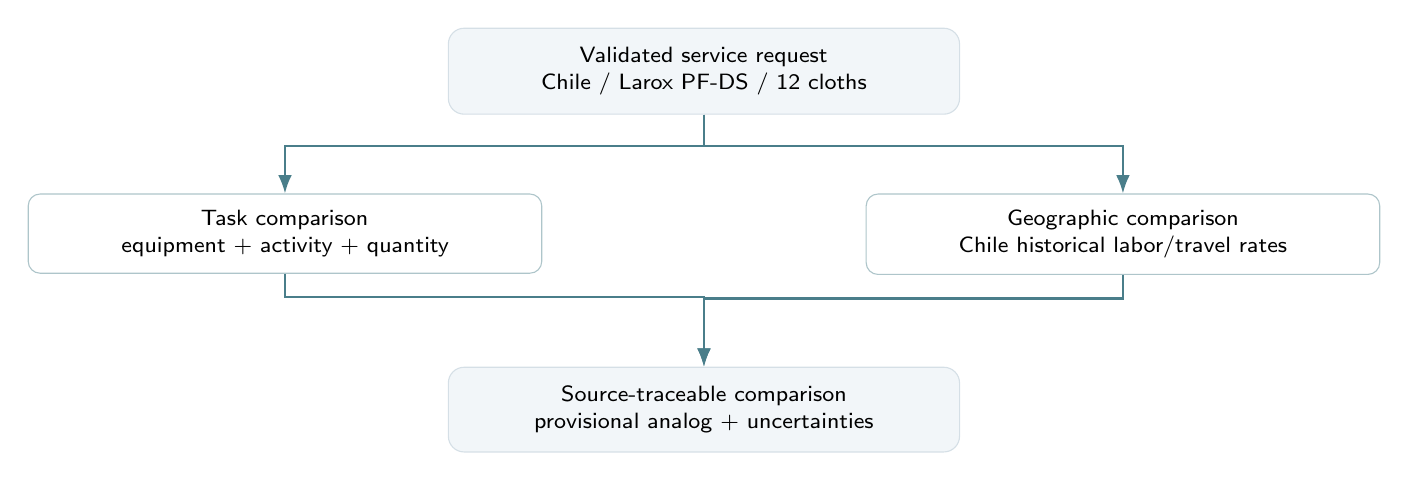
\begin{tikzpicture}[>=Latex,node distance=7mm,
 every node/.style={font=\sffamily\footnotesize},
 box/.style={draw=Rule,rounded corners=2mm,fill=Pale,align=center,text width=60mm,inner sep=7pt},
 smallbox/.style={draw=Sea!45,rounded corners=1.5mm,fill=white,align=center,text width=61mm,inner sep=6pt}]
\node[box] (q) {Validated service request\\Chile / Larox PF-DS / 12 cloths};
\node[smallbox,below left=10mm and -12mm of q] (t) {Task comparison\\equipment + activity + quantity};
\node[smallbox,below right=10mm and -12mm of q] (g) {Geographic comparison\\Chile historical labor/travel rates};
\node[box,below=32mm of q] (o) {Source-traceable comparison\\provisional analog + uncertainties};
\draw[->,thick,Sea] (q.south) -- ++(0,-4mm) -| (t.north);
\draw[->,thick,Sea] (q.south) -- ++(0,-4mm) -| (g.north);
\draw[->,thick,Sea] (t.south) -- ++(0,-3mm) -| (o.north);
\draw[->,thick,Sea] (g.south) -- ++(0,-3mm) -| (o.north);
\end{tikzpicture}
\end{center}

\subsection{05.7 --- Why the missing FSR-0027 source total remains missing}
The highest-ranked task analog, \code{FSR-0027}, describes a Swedish PF-DS intervention involving twelve filter cloths. Its service-cost summary stops during the fastening-clip row. Stage 04 preserved three complete cost-summary rows and separately stored priced material candidates. Stage 05 recovers additional documented material components \emph{only after checking} the original material-table headings, the source line, the currency and the arithmetic. A source-item signature avoids counting the same quantity, rate and amount twice when a material also appears in the summary.

The observed historical reconstruction was:

\begin{tabularx}{\textwidth}{@{}L{50mm}L{45mm}r@{}}
\toprule
\textbf{Component} & \textbf{Verified calculation / source} & \textbf{EUR}\\
\midrule
Travel & 4.9 h $\times$ 62; line 73 & 303.80\\
Labour & 8.4 h $\times$ 78; line 74 & 655.20\\
Filter cloths & 12 $\times$ 98; line 75 & 1,176.00\\
Fastening clips & 24 $\times$ 2.60; material line 43 & 62.40\\
Cleaning supplies & 1 lot $\times$ 18; material line 44 & 18.00\\
\midrule
\textbf{Provisional historical component sum} & \textbf{NOT the printed report total} & \textbf{2,215.40}\\
\bottomrule
\end{tabularx}

\begin{equation}
303.80 + 655.20 + 1176.00 + 62.40 + 18.00
= \boxed{2{,}215.40\;\mathrm{EUR}}.
\end{equation}

\textbf{Source identifiers actually returned by the program:} \code{FSR-0027:line:73}, \code{line:74}, \code{line:75}, \code{line:43}, and \code{line:44}; each entry also carries a \code{basis} recording whether it came from a reported cost-summary line or a priced material table supplement. The program classified the result as \code{PROVISIONAL_COMPONENT_SUM_NOT_SOURCE_TOTAL}.

\begin{warnbox}
\textbf{Never call this a source-printed invoice or a Chile quote.} FSR-0027 contains a truncated cost table, its recorded 8.4 work hours differ from the 8.75-hour activity window, and its Swedish prices do not establish local Chilean charges. The extracted sources also have a PF-DS cloth-count terminology ambiguity relative to the endless-cloth brochure. The correct status is a provisional, historically reconstructed comparator requiring source review.
\end{warnbox}

\subsection{05.8 --- Execute the required Chile demonstration in Windows PowerShell}
The user executed the following command from the project root. It calls the deterministic estimator directly; no LLM is asked to select the tool in this stage.

\begin{Verbatim}[fontsize=\footnotesize]
.\.venv\Scripts\python.exe -m metso_agent.estimation.cost_estimator `
  --country Chile `
  --equipment "Larox PF-DS tower press" `
  --task "filter cloth replacement" --quantity 12
\end{Verbatim}

The captured output stated:
\begin{Verbatim}[fontsize=\footnotesize]
Stage05 historical evidence comparison -- NOT A COMMERCIAL QUOTE
Target: 12 filter cloth replacement on Larox PF-DS
        tower press in Chile
Task analogs: ['FSR-0027', 'FSR-0014',
               'FSR-0031', 'FSR-0044']
Closest historical item sum: 2215.40 EUR
PROVISIONAL reconstruction -- NOT an invoice total or Chile price
Geographic comparator reports with supported hourly rates: 3
Site-specific budget: INSUFFICIENT EVIDENCE (no invented number)
Follow-up: What is the exact customer site in Chile?
Follow-up: Who supplies the replacement cloths?
\end{Verbatim}

\textbf{Interpretation.} The task-matching path, historical arithmetic, country-rate discovery, abstention behavior and clarification requirements all worked together. This is the most significant Stage 05 integration result. A credible answer includes a useful comparison but explicitly refuses to imply that it is a fully supported Chile budget.

\subsection{05.9 --- Inspect ranking results and the evidence-bearing JSON}
The program wrote the comparison into \code{local_cache/stage05_cost_comparison.json}. Its existence was confirmed by \code{Test-Path=True}, after which the user imported it using \code{ConvertFrom-Json} and inspected the individual fields. The top four observed task analogs were:

\begin{tabularx}{\textwidth}{@{}L{29mm}L{39mm}cY@{}}
\toprule
\textbf{Report} & \textbf{Country} & \textbf{Score} & \textbf{Relevance and limitation}\\
\midrule
FSR-0027 & Sweden & 20 & Closest 12-cloth PF-DS task; truncated summary.\\
FSR-0014 & Canada & 16 & Related PF-DS cloths; additional service work.\\
FSR-0031 & Finland & 16 & PF-DS cloths plus other work; VAT considerations.\\
FSR-0044 & Sweden & 10 & PF-DS work, bundled SEK price, not itemized.\\
\bottomrule
\end{tabularx}

These scores are deterministic \emph{ranking heuristic values}, not percentage probabilities, confidence intervals or empirically calibrated commercial similarity. In the generated object, \code{best_historical_analog.reconstructed} contained \code{amount=2215.40} and \code{currency=EUR}. The five components and their specific source lines were displayed separately. Most importantly, \code{site_specific_budget} remained JSON \code{null}; the explicit test \code{$null -eq $result.site_specific_budget} returned \code{True}.

\subsection{05.10 --- Inspect Chilean rates without borrowing their unrelated scopes}
Three Chilean reports contributed source-supported historical labor and travel rate observations:

\begin{tabularx}{\textwidth}{@{}L{24mm}L{49mm}r r L{19mm}@{}}
\toprule
\textbf{Report} & \textbf{Equipment / scope} & \textbf{Labor / h} & \textbf{Travel / h} & \textbf{Currency}\\
\midrule
FSR-0001 & ColumnCell inspection & 110 & 75 & USD\\
FSR-0015 & Filter Optimizer installation & 95 & 70 & USD\\
FSR-0034 & ColumnCell inspection & 110 & 80 & USD\\
\bottomrule
\end{tabularx}

The user's JSON inspection confirmed the presence of all three source IDs. These are \emph{observed past rates for other equipment and jobs}. They are not a current Chile PF-DS rate card. The engine therefore does not merge them into the EUR reconstruction. Nor does it use the bundled FSR-0035 amount as an hourly rate or the equipment-inclusive installation total in FSR-0015 as the price of a cloth change.

\subsection{05.11 --- Test a follow-up with a site and a named parts supplier}
The user then reran the estimator with two additional facts: \code{site=Antofagasta} and \code{parts_supplier=customer}. The call used \code{--site "Antofagasta" --parts-supplier customer}. The observed output still selected FSR-0027 first, preserved the provisional EUR reconstruction, and retained the status \code{INSUFFICIENT EVIDENCE} for the site-specific budget. The two earlier follow-up questions no longer appeared because these two fields had been supplied.

\textbf{What this confirms.} Request fields affect which clarifications are asked, without forcing an unjustified monetary answer. The CLI can process separate, explicit input configurations. \textbf{What this does not confirm.} It is not yet an interactive multi-turn AI conversation and it does not calculate a Chilean quote. The later conversational controller must preserve prior context when natural-language follow-up messages are provided.

\subsection{05.12 --- Dedicated unit tests: eighteen safeguards}
The user ran the Stage 05 test module explicitly; the terminal showed \textbf{18 passed in 0.25 seconds}. Each test used synthetic data and was designed to prevent a particular failure, as summarized below.

\begin{longtable}{@{}L{76mm}L{70mm}@{}}
\toprule
\textbf{Test identifier} & \textbf{Failure mode prevented or behavior verified}\\
\midrule\endfirsthead
\toprule\textbf{Test identifier} & \textbf{Purpose}\\
\midrule\endhead
{\footnotesize\ttfamily test\_\allowbreak decimal\_\allowbreak amounts\_\allowbreak are\_\allowbreak exact} & Exact line-item arithmetic with Decimal.\\
{\footnotesize\ttfamily test\_\allowbreak invalid\_\allowbreak line\_\allowbreak arithmetic\_\allowbreak rejected} & Reject contradictory quantity-rate-extension tuples.\\
{\footnotesize\ttfamily test\_\allowbreak unknown\_\allowbreak is\_\allowbreak not\_\allowbreak zero} & Do not substitute zero for missing numeric data.\\
{\footnotesize\ttfamily test\_\allowbreak non\_\allowbreak finite\_\allowbreak numeric\_\allowbreak rejected} & Reject non-finite monetary inputs.\\
{\footnotesize\ttfamily test\_\allowbreak mixed\_\allowbreak currency\_\allowbreak sum\_\allowbreak rejected} & Block mixed-currency addition.\\
{\footnotesize\ttfamily test\_\allowbreak same\_\allowbreak currency\_\allowbreak sum} & Permit a supported same-currency sum.\\
{\footnotesize\ttfamily test\_\allowbreak request\_\allowbreak rejects\_\allowbreak zero\_\allowbreak quantity} & Reject nonpositive service quantities.\\
{\footnotesize\ttfamily test\_\allowbreak request\_\allowbreak rejects\_\allowbreak invalid\_\allowbreak supplier} & Validate parts-supplier choices.\\
{\footnotesize\ttfamily test\_\allowbreak loader\_\allowbreak rejects\_\allowbreak duplicates} & Reject duplicate ledger report IDs.\\
{\footnotesize\ttfamily test\_\allowbreak original\_\allowbreak digest\_\allowbreak detects\_\allowbreak tamper} & Detect a source file changed since ingestion.\\
{\footnotesize\ttfamily test\_\allowbreak partial\_\allowbreak materials\_\allowbreak reconstructed\_\allowbreak without\_\allowbreak double\_\allowbreak count} & Supplement supported material lines in an incomplete case without duplicate components.\\
{\footnotesize\ttfamily test\_\allowbreak missing\_\allowbreak material\_\allowbreak currency\_\allowbreak header\_\allowbreak not\_\allowbreak supplemented} & Do not infer an unstated material-table currency.\\
{\footnotesize\ttfamily test\_\allowbreak printed\_\allowbreak total\_\allowbreak kept\_\allowbreak separate\_\allowbreak from\_\allowbreak reconstruction} & Preserve a printed total independently from reconstructed amounts.\\
{\footnotesize\ttfamily test\_\allowbreak exact\_\allowbreak equipment\_\allowbreak filter\_\allowbreak excludes\_\allowbreak pf\_\allowbreak without\_\allowbreak ds} & Distinguish PF from PF-DS when selecting analogs.\\
{\footnotesize\ttfamily test\_\allowbreak local\_\allowbreak rates\_\allowbreak keep\_\allowbreak original\_\allowbreak currency\_\allowbreak and\_\allowbreak provenance} & Preserve currency and source for local rate observations.\\
{\footnotesize\ttfamily test\_\allowbreak no\_\allowbreak site\_\allowbreak specific\_\allowbreak price\_\allowbreak is\_\allowbreak invented} & Withhold unsupported country-specific commercial amounts.\\
{\footnotesize\ttfamily test\_\allowbreak extracted\_\allowbreak line\_\allowbreak has\_\allowbreak source\_\allowbreak location} & Require source line traceability for cost evidence.\\
{\footnotesize\ttfamily test\_\allowbreak unpriced\_\allowbreak report\_\allowbreak keeps\_\allowbreak unknown} & Represent price absence as insufficient evidence, not free service.\\
\bottomrule
\end{longtable}

\textbf{Important qualification.} These tests validate specified functions and synthetic edge cases. They do not mean every one of the fifty historical service records has been human-validated, nor that a live quotation has been commercially approved.

\subsection{05.13 --- Whole-project regression: fifty-one passing tests}
The user next ran \code{python -m pytest -v} against the complete existing codebase. The real terminal transcript recorded \textbf{51 collected and 51 passed in 4.71 seconds}. Another quick run reported \textbf{51 passed in 10.86 seconds}. Variation in wall-clock time is not a functional failure; the important results are test collection and status.

\begin{tabularx}{\textwidth}{@{}Y r@{}}
\toprule
\textbf{Test group} & \textbf{Passing tests}\\
\midrule
Stage 05 cost estimation and evidence guards & 18\\
Stage 04 service parser & 12\\
Stage 03 product retrieval & 7\\
Stage 02 schema / provenance & 13\\
Stage 00 CLI smoke test & 1\\
\midrule
\textbf{Combined passing test count} & \textbf{51 / 51}\\
\bottomrule
\end{tabularx}

This is evidence that adding the estimation module did not break behavior exercised by earlier unit tests. It does not validate free-text tool routing, citation entailment, end-user conversational quality or commercial price accuracy. These remain later integration and evaluation tasks.

\subsection{05.14 --- Validate private output handling and identify residual publication risks}
The user ran \code{git check-ignore -v local_cache/stage05_cost_comparison.json}; the output mapped the comparison JSON to \code{.gitignore:60:local_cache/}. The broader Git status showed \code{raw/}, \code{docs/private/}, \code{local_cache/}, virtual environments, caches and package metadata as ignored. The \code{git ls-files} command displayed no tracked files in this local session.

\begin{warnbox}
\textbf{Unresolved safety item.} The seven-part private study PDF and TeX files were still shown as \code{??} at the repository root, not as ignored. Although untracked is not published, a future \code{git add .} could stage them. Move these private documents into an ignored location or explicitly ignore them before the first public commit. Also check for credentials or confidential excerpts in all proposed public files. \code{.gitignore} alone cannot remove files from an already-published Git history.
\end{warnbox}

\subsection{05.15 --- Acceptance decision and remaining work}
\begin{longtable}{@{}L{54mm}L{50mm}L{43mm}@{}}
\toprule
\textbf{Criterion} & \textbf{Observed evidence} & \textbf{Conclusion}\\
\midrule\endfirsthead
\toprule\textbf{Criterion} & \textbf{Observed evidence} & \textbf{Conclusion}\\
\midrule\endhead
Required input artifacts & Source TXT, ledger and three implementation files exist. & Verified on Windows.\\
Standalone estimator & CLI completed both requested argument sets. & Executed successfully.\\
Accurate historical reconstruction & Five components sum to EUR 2,215.40. & Arithmetic verified, source review pending.\\
Comparable PF-DS ranking & FSR-0027 ranked first with score 20. & Verified for demonstration request.\\
Country-specific rate discovery & Three Chilean rate-bearing FSRs found. & Verified, not scope-equivalent.\\
Currency protection & Explicit mixed-currency unit test passed. & Verified on synthetic cases.\\
Unpriced report handling & Unknown/None test passed. & Verified on synthetic cases.\\
No fabricated Chile budget & \code{site_specific_budget=null} and \code{True} check. & Verified live output.\\
Follow-up update & Known site/supplier removed corresponding questions. & Verified on repeat CLI run.\\
Stage 05 unit regression & 18/18 passed. & Complete for defined tests.\\
Whole project regression & 51/51 passed. & Complete for defined tests.\\
Generated JSON confidentiality & Ignore rule confirmed. & Local boundary confirmed.\\
Manual Stage 04 approval & Reference review still had Pending decisions. & \textbf{Open}.\\
Private report in repository root & PDF/TeX remained untracked, not ignored. & \textbf{Action required}.\\
True conversational agent & Requires intent routing and multi-turn LLM controller. & \textbf{Not Stage 05}.\\
Customer-ready commercial estimate & No current Chile/site-specific supporting evidence. & \textbf{Not established}.\\
\bottomrule
\end{longtable}

\begin{keybox}
\textbf{Stage 05 sign-off.} \textbf{Implementation, live demonstration and defined test suite: PASS.} The observed output correctly identifies the nearest historical work, rebuilds a defensible provisional source-component amount, preserves original currencies and citations, and declines to invent a Chile-specific site-visit budget. \textbf{Evidence certification and commercial suitability: NOT YET VERIFIED.} Manual adjudication of sensitive reports, actual customer-specific rate/scope confirmation and public-repository safety remain open. These are substantive trust boundaries, not test failures to conceal.
\end{keybox}

\subsection{Lessons learned and hand-off to Stage 06}
The central result is an operational separation of \emph{historical evidence}, \emph{verified arithmetic} and \emph{decision uncertainty}. A weak solution could have copied EUR 2,215.40 and labeled it the price in Chile, or averaged EUR and USD because both appeared near the desired work. The implemented estimator avoids those mistakes. It also shows why the highest-ranked report is not necessarily complete, why a source hash does not prove every extracted value, and why passing unit tests does not replace human review.

The next deliverable is a conversational controller that accepts the customer's original free-text request, chooses brochure search, service comparison or both, and asks for relevant missing information without requiring the user to pass command-line mode flags. Stage 07 must then verify that final narrative claims and citations actually follow from the evidence rather than relying on lexical similarity or apparently precise numerical formatting.

\textbf{Immediate practical priorities:} finalize manual review for FSR-0027 and other high-impact reports; remove the private report files from the unignored repository root; preserve the fully passing 51-test baseline; and integrate the product retriever and estimator with a bounded, auditable tool-calling agent. The binding deadline and public-code/video/independent interview requirements remain separate completion gates.

\vspace{4mm}
\begin{center}
{\sffamily\color{Gray}\footnotesize END OF PART VIII -- STAGE 05 EVIDENCE-BASED COST ESTIMATION}\\[2mm]
{\sffamily\bfseries\color{Navy}AG is your G!}
\end{center}

\clearpage
\section{Stage 06 --- Build the autonomous conversational agent controller}
\label{sec:executed-stage06}

\begin{keybox}
\textbf{Execution verdict, 19 October 2026.} The autonomous controller was implemented and exercised through both a synthetic unit-test suite and a live OpenAI API session. The user-reported Windows run yielded \textbf{12/12 Stage 06 tests} and \textbf{63/63 tests across the project}; the local dependency check recognized the product retriever and a 50-report service ledger. A live \code{gpt-5-mini} session automatically invoked \code{search_product_brochures} for the changing-feed question and \code{compare_service_costs} for the Chile service-budget question. A combined request invoked \emph{both} tools, and follow-up turns preserved site and parts-supply context. \textbf{The engineering Stage 06 milestone is reached for the observed cases, but the agent is not yet fully claim-validated or commercially approved.}
\end{keybox}

\subsection{06.1 --- The operational gap between standalone tools and a working agent}
At the end of Stage 05, the product retriever and service-cost estimator could be executed individually from PowerShell. That proved the evidence mechanisms, but a Metso salesperson would still have needed to recognize the intent, choose a command, supply the right parameters, and interpret the output. The assignment explicitly requires the \emph{assistant itself} to select the right action from a natural-language customer question. Stage 06 therefore connected the already tested components through a conversational controller rather than building a second retrieval method or recalculating money inside the language model.

\textbf{The engineering objective was fivefold:} (1) accept unstructured English messages; (2) let an LLM select one or more approved tools; (3) validate the selected tool and arguments before local execution; (4) synthesize an answer with evidence, limitations and a useful question when information is missing; and (5) preserve relevant conversational context over follow-up turns. The implementation was intentionally a command-line program: a graphical interface is not required by the brief.

\subsection{06.2 --- The existing architecture reused in Stage 06}
The implementation maintained the source-of-truth boundaries established in the earlier chapters. Brochure search is supported by the 12 Markdown/PDF product pairs; service comparisons are supported by the 50 historical FSRs and the private structured ledger. The LLM handles language, routing and response phrasing, while Python remains responsible for lookup and exact money arithmetic.

\begin{center}
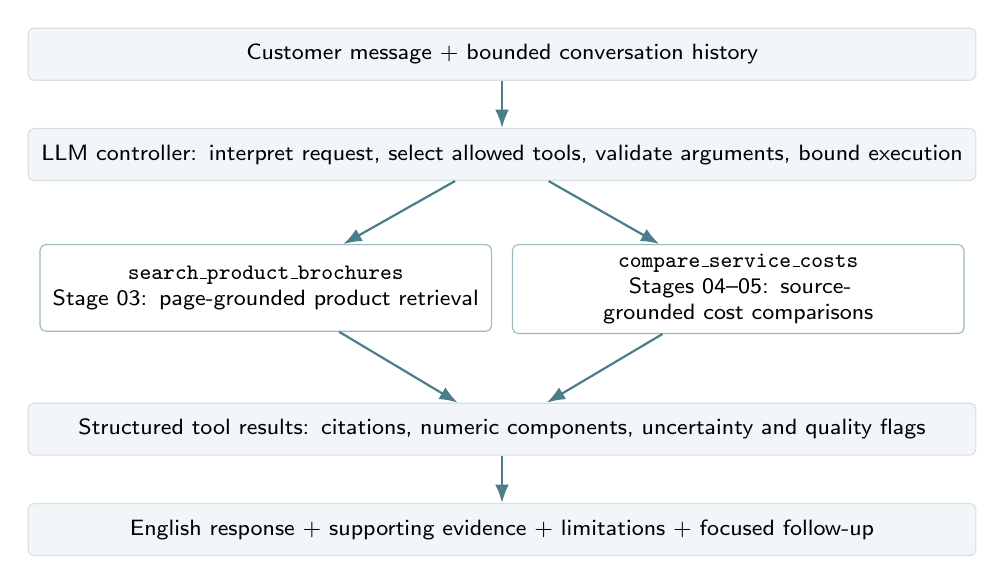
\begin{tikzpicture}[node distance=6mm and 8mm, every node/.style={font=\footnotesize\sffamily}, box/.style={draw=Rule, rounded corners=2pt, fill=Pale, text width=11.8cm, align=center, minimum height=0.66cm}, sourcebox/.style={draw=Sea!55, rounded corners=2pt, text width=5.5cm, align=center, minimum height=1.1cm}, arr/.style={-Latex, thick, draw=Sea}]
\node[box] (user) {Customer message + bounded conversation history};
\node[box, below=of user] (ctrl) {LLM controller: interpret request, select allowed tools, validate arguments, bound execution};
\node[sourcebox, below=8mm of ctrl,xshift=-3.0cm] (prod) {\texttt{search\_product\_brochures}\\Stage 03: page-grounded product retrieval};
\node[sourcebox, below=8mm of ctrl,xshift=3.0cm] (cost) {\texttt{compare\_service\_costs}\\Stages 04--05: source-grounded cost comparisons};
\node[box, below=9mm of prod,xshift=3.0cm] (result) {Structured tool results: citations, numeric components, uncertainty and quality flags};
\node[box, below=of result] (answer) {English response + supporting evidence + limitations + focused follow-up};
\draw[arr] (user) -- (ctrl);
\draw[arr] (ctrl) -- (prod);
\draw[arr] (ctrl) -- (cost);
\draw[arr] (prod) -- (result);
\draw[arr] (cost) -- (result);
\draw[arr] (result) -- (answer);
\end{tikzpicture}
\end{center}

This separation matters because a plausible-sounding LLM response is not itself proof of a supported product specification or service rate. For example, the provisional EUR~2,215.40 analog is calculated from report-backed components in the estimator, not invented as a completion by the model. The final narrative can still overstate a conclusion; that remaining risk belongs to Stage 07.

\subsection{06.3 --- Project files created, and why each exists}
The user added the Stage 06 module under the established editable Python package without replacing the previous product or service engines.

\begin{tabularx}{\textwidth}{@{}L{53mm}Y@{}}
\toprule
\textbf{Path} & \textbf{Responsibility and rationale}\\\midrule
{\footnotesize\path{src/metso_agent/agent/tools.py}} & Tool adapters joining LLM-compatible input contracts to the independently tested product retrieval and service-cost engines.\\
{\footnotesize\path{src/metso_agent/agent/controller.py}} & Conversation state, Responses API interaction, bounded tool-calling loop, tool-name checks, argument validation and safe error handling.\\
{\footnotesize\path{src/metso_agent/agent/chat.py}} & Terminal entry point, local dependency check, live chat loop, verbose tool trace and the \code{exit} command.\\
{\footnotesize\path{src/metso_agent/agent/__init__.py}} & Makes \code{agent} an importable Python package.\\
{\footnotesize\path{tests/test_agent_controller.py}} & Twelve offline tests for routing, combined questions, history, malformed inputs, API errors and tool budgets.\\
{\footnotesize\path{docs/agent_controller.md}} & Describes the routing architecture, execution contract, safeguards, limitations and repeatable commands. The presence and complete content of this file were \emph{not} independently proven by the captured transcript.\\
\bottomrule
\end{tabularx}

\subsection{06.4 --- 06.1--06.2: verify the Windows interpreter and installation}
The operator used the existing project root under \path{C:/1.Personality/2.Scaned/CV/Job2/Job/87.Metso _ AI Solution Engineer/interview/project}. An initial pasted command had accidentally concatenated \code{Set-Location} and the PowerShell activation expression; PowerShell rejected the malformed command. A corrected standalone \code{Set-Location -LiteralPath} succeeded. This was a command-entry issue, not a broken environment.

\begin{examplebox}
\textbf{Observed environment:} \code{Python 3.12.4}; \code{openai 2.54.0}; \code{python-dotenv 1.2.4}; \code{pydantic 2.14.1} appears in the dependency report. A subsequent \code{pip install} call reported \emph{Requirement already satisfied} for the OpenAI and dotenv packages. \code{Test-Path} returned \code{True} for \code{tools.py}, \code{controller.py}, \code{chat.py} and \code{test_agent_controller.py}.\\[3pt]
\textbf{Reason:} isolating dependencies under \code{.venv} makes the Windows development environment consistent and prevents system-wide package changes from being mistaken for project correctness.
\end{examplebox}

\subsection{06.5 --- 06.3: register only the two required tools}
The live agent exposes exactly the two required decision paths at this milestone:
\begin{itemize}
\item \code{search_product_brochures}: searches the supplied brochure corpus and returns product passages with document/page identifiers, suitable for questions about Larox filters and Filter Optimizer.
\item \code{compare_service_costs}: accepts structured service-request fields, selects historical task and geographic comparators, and returns traceable monetary components, the estimate status, warnings and unanswered questions.
\end{itemize}
The controller is allowed to invoke both tools in the same turn. It is \emph{not} required to invent a product price when a product question is asked, or to search brochures simply because a service record mentions Larox. Tool names and input fields function as a contract; the LLM does not acquire arbitrary Python execution privileges. The optional flotation-analysis tool was not demonstrated as part of Stage 06 and is not claimed as completed here.

\subsection{06.6 --- 06.4: implement a bounded function-calling controller}
The \code{controller.py} program communicates with the OpenAI Responses API, supplies the approved tool schemas, validates tool-call requests, executes local tools, and returns their outputs so the model can formulate a response. The controller keeps a bounded session history for natural follow-ups rather than asking the user to retype an entire question after every clarification. Tool-result context and final response text are different trust domains: retrieved evidence informs the answer but should not be accepted as instructions directing the agent's behavior.

\begin{tabularx}{\textwidth}{@{}L{49mm}Y@{}}
\toprule
\textbf{Safety or robustness measure} & \textbf{Reason for the implementation choice}\\\midrule
Approved tool names only & Reject calls to functions outside the authorized sales-assistant operations.\\
Strict input schema validation & Reject unknown fields, invalid quantities and malformed requests before reading local sources.\\
Bounded tool-call budget & Prevent uncontrolled recursion, repeated API usage and non-terminating action loops. The code package was designed around a small fixed execution budget.\\
Limited conversation history & Preserve relevant customer parameters without unnecessarily growing the context or repeatedly transmitting bulky tool outputs.\\
Safe API-failure handling & Report a recoverable failure class instead of displaying sensitive internal exception details to the customer.\\
Local computation boundary & Preserve \code{Decimal} money arithmetic, currency checks and source references in the deterministic estimator.\\
Explicit external-data switch & Live mode requires \code{--allow-external-evidence}; the local dependency test runs without an external request.\\
\bottomrule
\end{tabularx}

\subsection{06.7 --- 06.5: the twelve targeted offline tests}
The user executed the following command in the project's Python environment:
\begin{examplebox}
\small\ttfamily
.\textbackslash.venv\textbackslash Scripts\textbackslash python.exe -m pytest tests/test\_agent\_controller.py -v
\end{examplebox}
The recorded output collected \textbf{12 items}, and every item was marked \code{PASSED}; elapsed test time was \textbf{3.13 seconds}. The descriptions below preserve the scope of the actual test names, while avoiding the mistaken claim that mock-driven tests establish live-model reliability.

\begin{longtable}{@{}L{8mm}L{68mm}L{64mm}@{}}
\toprule
\textbf{No.} & \textbf{Test case from the Windows run} & \textbf{Specific behavior covered}\\\midrule\endfirsthead
\toprule\textbf{No.} & \textbf{Test case} & \textbf{Behavior}\\\midrule\endhead
1 & Product tool routed from natural language & Product-related text selects the retrieval adapter.\\
2 & Cost tool routed and budget remains null & A cost request selects the service tool without inventing a site price.\\
3 & Combined question can call both tools & Multi-intent requests can invoke product and service tools.\\
4 & Follow-up carries chat history, not private tool results & Conversational continuity while limiting carried evidence payload.\\
5 & Bounded tool calls fail closed & An exceeded tool budget is handled safely.\\
6 & API failure reports only class name & Error handling does not leak a detailed exception trace.\\
7 & Invalid argument or unknown tool rejected without crash & Defensive dispatch handles malformed calls.\\
8 & Product arguments reject extra properties & Unapproved fields are rejected before source reads.\\
9 & Service request rejects unknown quantity & An invalid service quantity is not accepted as a real estimate.\\
10 & API tool schemas are strict & Declared argument contracts are enforceable.\\
11 & Blank message rejected & Empty user input is not treated as a valid task.\\
12 & Failed API turn does not add session history & Failed operations do not silently pollute the next conversation turn.\\
\bottomrule
\end{longtable}

\subsection{06.8 --- 06.6: whole-project regression and no-network smoke check}
After the dedicated suite, the user ran \code{python -m pytest -v}. The terminal collected \textbf{63 tests}, all passed in \textbf{4.31 seconds}. A prior quick run also reported \textbf{63 passed in 11.74 seconds}. Together with Stage 06, the test inventory is:

\begin{tabularx}{\textwidth}{@{}Y r@{}}
\toprule
\textbf{Test group} & \textbf{Tests passed}\\\midrule
Stage 06 autonomous agent controller & 12\\
Stage 05 deterministic cost estimator & 18\\
Stage 04 historical service parser & 12\\
Stage 03 brochure retrieval & 7\\
Stage 02 typed data contracts & 13\\
Stage 00 CLI smoke test & 1\\\midrule
\textbf{Total} & \textbf{63 / 63}\\\bottomrule
\end{tabularx}

The independent no-network check also succeeded:
\begin{examplebox}
\footnotesize\ttfamily
Checking local-only dependencies (no network calls)...\\
Product retrieval usable: True\\
Service ledger readable: 50 reports\\
Check completed without external API calls.
\end{examplebox}

\textbf{Why both checks matter.} Unit tests verify controlled cases, while the local check verifies that the new controller can reach the already prepared retrieval and service artifacts in the real project. Neither proves that a live LLM will always choose correctly or that its final prose will be faithful; those require observed live examples and Stage 07 validation.

\subsection{06.9 --- 06.7--06.9: employer clarification, billing and API configuration}
The official assignment allows use of an LLM API. On 19 October 2026, the user also received an explicit clarification from the Metso contact, Tarek Ali, describing the supplied assignment material as public/non-secret and indicating that an enterprise-specific OpenAI agreement was not expected for this exercise. This resolved the previously open ambiguity about using an ordinary external model API with the provided evidence for this assignment. The original submission rule \emph{not to publish the supplied data directory or any API credentials} still applies.

Initially the live chat command returned \code{Missing OPENAI_API_KEY in private .env}. This was a configuration failure, not a tool-routing failure. The user subsequently configured a private \code{.env} containing an API key and the selected model identifier \code{gpt-5-mini}. A diagnostic printed \code{API key configured: True} and \code{Model: gpt-5-mini} without printing the secret. The user then made a minimal Responses API request with an ordinary public prompt, \code{store=False}, and received the exact result \code{CONNECTED}. This confirmed authentication, billing/model access and end-to-end API reachability for that test.

The user chose an initial USD~5 API-credit purchase and asked for automatic recharging to be disabled; the supplied terminal transcript \emph{does not independently show the final billing toggle state}. Recording \emph{Auto-reload disabled} as a verified fact would therefore exceed the evidence. The environment ignore rule was verified for \code{.env}; the secret itself was not reproduced in this report.

\subsection{06.10 --- 06.10--06.11: live product-routing demonstration}
The operator started the live console with:
\begin{examplebox}
\small\ttfamily
.\textbackslash.venv\textbackslash Scripts\textbackslash python.exe -m metso\_agent.agent.chat --allow-external-evidence --verbose
\end{examplebox}
The application displayed \code{Metso Evidence Agent / Stage 06} and prompted for \code{You >}. The exact required product question was entered: ``We have Larox pressure filters but performance drops whenever our feed grade changes.'' The runtime trace stated \textbf{\code{Tools used: search_product_brochures}}.

The model's answer identified the Metso Filter Optimizer as relevant, cited \code{filter-optimizer} page~2, and referenced Larox PF-DS page~2 for automatic cycles and page~3 for cloth-cleaning context. It also cited the two broader Larox PF brochures for cloth/plate options. The answer suggested checking control settings, cleaning and material/filter configuration, and asked for the exact Larox model, the nature of feed variability and the control mode.

\begin{keybox}
\textbf{Observed success:} The agent selected the product tool automatically and produced a brochure-referenced recommendation plus a targeted follow-up.\\[3pt]
\textbf{Observed limitation:} It opened by asserting that this behavior is ``common when slurry properties change faster than the filter control or media can adapt.'' This is a plausible hypothesis, but the customer's single sentence does not prove a mechanism. It also drew on PF-DS-specific information before the customer's installed variant had been identified. These statements should be qualified as investigation hypotheses and model-dependent options in Stage 07.
\end{keybox}

\subsection{06.11 --- 06.12: live Chile service-budget demonstration}
The mandatory service prompt was entered: ``A customer in Chile needs 12 filter cloths replaced on a Larox PF-DS tower press. What should I budget for the service visit?'' The observed trace stated \textbf{\code{Tools used: compare_service_costs}}. The agent selected \code{FSR-0027}, a Swedish 12-cloth Larox PF-DS service case, as its strongest operational analog. It preserved the provisional reconstruction status and cited individual source lines rather than falsely presenting an incomplete report as a verified invoice.

\begin{tabularx}{\textwidth}{@{}Y r r r@{}}
\toprule
\textbf{FSR-0027 documented component} & \textbf{Quantity} & \textbf{EUR/unit} & \textbf{EUR total}\\\midrule
Travel, line 73 & 4.9 & 62.00 & 303.80\\
Technician labor, line 74 & 8.4 & 78.00 & 655.20\\
Filter cloths, line 75 & 12 & 98.00 & 1,176.00\\
Fastening clips, line 43 & 24 & 2.60 & 62.40\\
Cleaning supplies, line 44 & 1 & 18.00 & 18.00\\\midrule
\textbf{Reconstructed historical components} & & & \textbf{2,215.40}\\\bottomrule
\end{tabularx}

The model explicitly described this as an internal historical planning reference from Sweden, not the commercial price in Chile. It disclosed truncated cost lines, lack of a printed total, incomplete travel/local tax assumptions and the PF-DS endless-cloth versus multiple-cloth terminology concern. It kept alternative totals in their original currencies: Finland EUR~2,580.44, Canada CAD~4,367 and Sweden SEK~19,850. It asked for the exact Chile site and the party providing the cloths.

\textbf{The important boundary held:} the estimator did not supply a verified Chile site budget (\code{site_specific_budget = null}), and the model's answer did not convert historical amounts into an unsupported binding quote. This test demonstrates operational routing and appropriately caveated presentation, not commercial approval of EUR~2,215.40.

\subsection{06.12 --- 06.13: follow-up, site and customer-supplied parts}
The user then added: ``The customer site is in Antofagasta, Chile, and the customer will supply the 12 replacement filter cloths.'' The trace again showed \code{compare_service_costs}. The assistant retained the earlier equipment, task and quantity and removed the historical cloth-purchase line from a \emph{new comparison calculation}:
\[
\underbrace{303.80}_{\text{travel}} + \underbrace{655.20}_{\text{labor}} + \underbrace{62.40}_{\text{clips}} + \underbrace{18.00}_{\text{supplies}} = \boxed{1{,}039.40\ \text{EUR}}.
\]
The separate historical all-component amount of EUR~2,215.40 was not erased; the EUR~1,039.40 value is a provisional recalculation after \emph{excluding customer-supplied cloths}. It remains based on Swedish historic rates and is \emph{not} a verified Chile job price. The assistant asked where technicians would originate, correctly identifying another influential unknown.

\begin{warnbox}
\textbf{Remaining interpretation risk.} Excluding the cloth \emph{purchase cost} is reasonable only because the customer says they will supply the cloths. This does not establish that all other labor, clip and cleaning charges are complete or currently applicable, or that a narrower commercial range can definitely be computed after one more answer. In later live responses the model sometimes promised a ``tighter planning range'' despite continuing insufficient evidence. This expectation must be constrained by the evidence gate in Stage 07.
\end{warnbox}

\subsection{06.13 --- 06.13--06.14: combined-intent and multi-turn behavior}
The user tested a compound message seeking a product solution for variable feed conditions \emph{and} historical cost evidence for twelve PF-DS cloths in Chile. The runtime trace explicitly recorded:
\begin{examplebox}
\small\ttfamily
Tools used: search\_product\_brochures, compare\_service\_costs
\end{examplebox}
The assistant combined citations to the Filter Optimizer and PF-DS brochures with the FSR-0027 cost breakdown, retained the Antofagasta/customer-supplied cloth context, and repeated the recalculated provisional EUR~1,039.40 reference. This is direct live evidence that routing was \emph{not} hard-coded as exactly one intent per message.

A subsequent sequence continued with ``I need a service cost estimate for replacing 12 filter cloths,'' ``It is a Larox PF-DS in Chile,'' and ``The site is in Antofagasta and the customer provides the cloths.'' In each observed turn the service tool was selected; the model retained the twelve-cloth request and the previously established site/supplier facts. The user ended the session by typing \code{exit}; the console displayed \code{Session ended.}.

\textbf{A precise caveat about the test:} these were conducted in the \emph{same live session} as the earlier Chile scenario. The short first message already inherited Antofagasta and customer-supplied cloths from prior turns. That verifies carry-over across turns, but it is not an independent demonstration of eliciting all missing information from an empty conversation. For an unbiased first-turn test, start a fresh \code{chat.py} session or reset conversation state.

\subsection{06.14 --- Agent traces and explicit comparison of requested vs. observed behavior}
\begin{longtable}{@{}L{43mm}L{60mm}L{43mm}@{}}
\toprule
\textbf{Scenario} & \textbf{Observed tool and output} & \textbf{Assessment}\\\midrule\endfirsthead
\toprule\textbf{Scenario} & \textbf{Observed behavior} & \textbf{Assessment}\\\midrule\endhead
Larox feed-change request & \code{search_product_brochures}; Filter Optimizer and Larox page references. & \textbf{Pass for tool routing}; causal phrasing needs a guard.\\
Chile 12-cloth cost request & \code{compare_service_costs}; FSR-0027; provisional EUR~2,215.40. & \textbf{Pass for routing/arithmetic}; commercial price withheld.\\
Known site and parts supplier & \code{compare_service_costs}; Antofagasta; customer cloths removed from new component sum. & \textbf{Pass for context}; provisional EUR~1,039.40 remains a Swedish analog.\\
Combined product and cost request & Both named tools explicitly invoked in the trace. & \textbf{Pass for multi-tool action}.\\
Three-message follow-up sequence & Service tool called repeatedly; prior scenario fields carried forward. & \textbf{Pass for same-session context}, not a fresh-session clarification test.\\
Program termination & \code{exit} produced \code{Session ended.} & \textbf{Pass for interactive CLI exit}.\\
Refusal of unsupported Chile quote & \code{site_specific_budget=null} remained explicit in narrative. & \textbf{Pass for observed case}; generalized validation pending.\\
Optional flotation question & No Stage 06 live output in this transcript. & \textbf{Not tested / optional}.\\
\bottomrule
\end{longtable}

\subsection{06.15 --- Source discipline, Git status and controlled API use}
The operator verified \code{git check-ignore -v .env}, returning \code{.gitignore:63:.env}, and \code{git check-ignore -v local_cache/service_ledger.json}, returning \code{.gitignore:60:local_cache/}. The final \code{git status --short --ignored} showed \code{.env}, \code{raw/}, \code{docs/private/}, \code{local_cache/}, virtual environments and Python cache directories as ignored. \code{git ls-files} returned an empty list: nothing had yet been committed or tracked in that local repository.

\begin{warnbox}
\textbf{Public-release blocker still open.} The eight-part study PDF and TeX files remained \code{??} at the repository root. Untracked does \emph{not} mean published, but it does mean a broad \code{git add .} could stage them. Move them into an ignored private folder or explicitly exclude them before staging. Validate the staged file list and the full history before making the GitHub repository public. The employer's clarification permitting an external LLM API does not override the official request to omit \code{data/} and secret keys from the public submission.
\end{warnbox}

The user confirmed the API could be reached with a harmless test prompt before sending selected source excerpts in live mode. No actual secret key was included in the supplied test transcript or in this report. For the recording, show tool names and evidence IDs, but not the contents of \code{.env}, account billing information or private local paths beyond what is necessary to explain setup.

\subsection{06.16 --- Stage 06 sign-off, limits and hand-off to Stage 07}
\begin{longtable}{@{}L{55mm}L{50mm}L{41mm}@{}}
\toprule
\textbf{Acceptance requirement} & \textbf{Recorded evidence} & \textbf{Judgment}\\\midrule\endfirsthead
\toprule\textbf{Requirement} & \textbf{Evidence} & \textbf{Judgment}\\\midrule\endhead
New module exists and is importable & Four \code{Test-Path} results were \code{True}; 12 tests ran. & \textbf{Verified}.\\
Twelve Stage 06 unit tests & 12 passed in 3.13 s. & \textbf{Verified}.\\
Whole-project regression & 63 passed in 4.31 s (verbose run). & \textbf{Verified}.\\
Local evidence integrations & Product retrieval usable, ledger 50 reports. & \textbf{Verified}.\\
LLM API connection & \code{CONNECTED} using \code{gpt-5-mini}. & \textbf{Verified}.\\
Automatic product routing & Product prompt called brochure tool. & \textbf{Verified for example}.\\
Automatic service routing & Chile prompt called cost tool. & \textbf{Verified for example}.\\
Combined-tool request & Live trace explicitly named both tools. & \textbf{Verified for example}.\\
Multi-turn continuity & Site/supplier persisted in same live chat. & \textbf{Verified within session}.\\
Monetary provenance and boundaries & EUR~2,215.40 historical; EUR~1,039.40 without cloths; Chile budget null. & \textbf{Verified as provisional output}.\\
Fully supported final wording & Some causal/compatibility and future-range language is too strong. & \textbf{Requires Stage 07}.\\
Independent cold-start clarification & Not exercised in a reset session. & \textbf{Not yet verified}.\\
Manual review of high-impact FSR fields & Prior \code{stage04_gold_review.md} decisions were still pending. & \textbf{Open}.\\
Public Git repository safety & Private study PDF/TeX untracked at root; no commits yet. & \textbf{Open}.\\
Final published deliverables & No public code/video links or Recright completion in this evidence. & \textbf{Not established}.\\
\bottomrule
\end{longtable}

\begin{keybox}
\textbf{Stage 06 engineering conclusion: PASS for the required autonomous conversational workflows observed.} The application is now a functioning tool-calling CLI rather than two standalone commands. Both mandatory customer prompts route correctly, a compound query invokes both tools, and same-session clarifications influence the output. The controller's twelve dedicated tests and the full 63-test project suite passed. \textbf{Not a blanket reliability guarantee:} evidence entailment, unsupported causal language, premature promises of numeric refinement, human validation of sensitive FSRs and final publication safety remain outside this stage's verified completion.
\end{keybox}

\textbf{What I learned.} Autonomy is operationally useful only when paired with clear tool boundaries. The model can infer customer intent, but tool outputs remain the only permitted evidence for product capabilities and service costs. A passed routing test is weaker than a source-supported answer; and a source-supported historical amount is weaker than a justified current customer quote. The Antofagasta follow-up illustrated both strengths and remaining risks: relevant context was retained, and the customer-supplied cloth line was excluded transparently, but the remaining EUR amount still derives from a Swedish precedent rather than Chile-specific verified pricing.

\textbf{Immediate continuation.} Stage 07 should verify claim-to-citation support; prohibit unsupported root-cause statements and guarantees; enforce unknown-value and currency safety in final prose; constrain promises of a ``tighter'' range to cases where additional data genuinely supports it; treat retrieved text as untrusted instructions; and test fresh-session clarifications. After that, prioritize the clean public-code package, a 5--7 minute recorded walkthrough, and the separate Recright submission by \textbf{20 October 2026 at 23:59 Helsinki time}. No evidence in the provided transcript establishes that these delivery requirements have already been completed.

\vspace{4mm}
\begin{center}
{\sffamily\color{Gray}\footnotesize END OF PART IX -- STAGE 06 AUTONOMOUS CONVERSATIONAL AGENT}\\[2mm]
{\sffamily\bfseries\color{Navy}AG is your G!}
\end{center}


\clearpage
\section{Stage 07 --- Validate claims, source boundaries, and uncertainty}
\begin{keybox}
\textbf{Engineering objective.} Insert a deterministic post-generation evidence gate between the autonomous Stage 06 controller and the customer-facing response. The gate must check references and supported monetary figures against the \emph{actual tool results from the current turn}, decline selected unsupported claims, and prevent rejected prose from entering the conversation history. \textbf{The observed result is 16/16 Stage 07 tests and 79/79 project tests passing on Windows after integration.} Live demonstrations \emph{after} the patch, a full manual claim-entailment audit and the release audit have not yet been evidenced.
\end{keybox}

\subsection{07.1 --- Why a working tool-calling agent still needs a validation boundary}
The Stage 06 controller already routed customer questions to two independently tested local tools: \code{search_product_brochures} for product evidence and \code{compare_service_costs} for historical service costs. The live demonstrations showed correct tool choices and cited historical evidence. Nevertheless, the language model was still responsible for transforming those tool results into free-form English. That transformation is a separate reliability boundary: it can overstate a hypothesis, attach a real citation to a claim that the cited source does not support, or promote an old reconstructed expense into a current commercial quotation.

For the Larox complaint, the first live response described a particular slurry/control adaptation mechanism as ``common'' even though the customer had not supplied evidence establishing that mechanism. For the Chile cloth-replacement question, the controller correctly displayed an \emph{EUR 2,215.40 provisional Swedish historical reconstruction}, while an unsupported confirmed Chilean quote would have been wrong. A follow-up in which the customer supplied the cloths yielded \emph{EUR 1,039.40} after subtracting EUR 1,176.00, but that new value was still a historical arithmetic comparator, not a Chile-specific commercial price. These observed risks supplied concrete reasons for adding Stage 07.

\textbf{Trust distinction.} A tool's correct answer is a structured observation. The final model-written sentence is a new claim requiring its own check. Correct tool selection and passing arithmetic unit tests do not automatically guarantee that the final narrative preserves source scope, qualification, currency or uncertainty.

\subsection{07.2 --- Scope and source boundaries carried forward from earlier stages}
The final-answer guard was designed as a small new component, not a replacement for the existing data, retrieval or cost-calculation logic. The following boundaries remained unchanged:
\begin{longtable}{@{}L{37mm}L{65mm}L{43mm}@{}}
\toprule
\textbf{Evidence domain} & \textbf{Legitimate claims} & \textbf{Claims to avoid}\\\midrule\endfirsthead
\toprule\textbf{Domain} & \textbf{Supported use} & \textbf{Unsafe shortcut}\\\midrule\endhead
Product brochures & Capabilities and specifications linked to a retrieved brochure identifier and page. & Unverified equipment compatibility, quantified savings or physical diagnosis.\\
Historical service reports & Identified visits, observed monetary lines and explicitly labeled reconstructions. & Invented current prices, fabricated site-specific quotes or treating incomplete invoices as complete.\\
Flotation CSV (optional) & Computed descriptive frequencies and sample statistics, if this optional tool is actually implemented. & Contractual acceptance limits or causal explanations inferred from descriptive data alone.\\
Agent conversation context & Prior customer-supplied facts such as site, equipment and parts supplier. & Treating previous model guesses as newly verified source evidence.\\
\bottomrule
\end{longtable}

The Stage 07 implementation concentrates on checks that can be made deterministically with the existing tool payloads. Full semantic verification of industrial claims, automatic product-compatibility assessment and production-quotation authorization are explicitly outside its present capabilities.

\subsection{07.3 --- Files added and the safe integration strategy}
The Stage 07 code-only package introduced the following artifacts. They were merged into the existing project; earlier schema, retrieval, ingestion and estimator implementations were retained.
\begin{longtable}{@{}L{70mm}L{75mm}@{}}
\toprule
\textbf{Path under project root} & \textbf{Purpose}\\\midrule\endfirsthead
\toprule\textbf{Path} & \textbf{Purpose}\\\midrule\endhead
\path{src/metso_agent/validation/response_guard.py} & Pure validator for supported citations, monetary values and selected prohibited statements.\\
\path{src/metso_agent/validation/__init__.py} & Marks the importable validation package.\\
\path{tests/test_response_guard.py} & Sixteen isolated, synthetic tests, including controller enforcement.\\
\path{scripts/apply_stage07_guard.py} & Narrow, layout-sensitive patch for the Stage 06 controller and CLI.\\
\path{docs/response_validation.md} & Design decisions, limitations, run commands and manual-review procedure.\\
\path{STAGE07_README.md} & Short operator hand-off and package instructions.\\
\bottomrule
\end{longtable}

\textbf{Why a patch script instead of copying a replacement controller?} The user's working Stage 06 already contained the verified function-calling loop and conversation state. Replacing its entire file with a generic template risked erasing behavior and previous fixes. The patch script instead searches for a small set of exact code snippets, aborts if the expected source layout is different, and writes original-file backups under the ignored \code{local_cache/stage07_backups/} path before applying changes. This supports rollback and makes the integration observable rather than silent.

\subsection{07.4 --- The observed first test run: diagnose rather than conceal the failure}
At the start of the recorded Stage 07 session, the user activated the project's virtual environment and confirmed \textbf{Python 3.12.4}. The initial complete test command was:
\begin{examplebox}
\footnotesize\ttfamily
.\textbackslash.venv\textbackslash Scripts\textbackslash python.exe -m pytest -q
\end{examplebox}

That initial run reported \textbf{77 passed and 2 failed} in 5.12 seconds. The failures were:
\begin{itemize}
\item \path{test_controller_enforcement_prevents_history_pollution}
\item \path{test_controller_enforcement_permits_supported_answer}
\end{itemize}
Both failed before validation could occur, for the same reason:
\begin{examplebox}
\footnotesize\ttfamily
TypeError: AgentController.\_\_init\_\_() got an unexpected\newline
keyword argument 'enforce\_evidence\_guards'
\end{examplebox}

\textbf{Diagnosis.} The test package had been copied into the project, but the Stage 06 \code{AgentController} constructor had not yet been extended with the opt-in evidence-guard flag. This was an integration-order problem, not evidence that the validator's monetary arithmetic or source checks were incorrect. The remaining 77 tests passed; the appropriate corrective action was to run the intended integration script, not to reinstall dependencies or weaken the tests.

\subsection{07.5 --- Apply the guard and preserve the previous working version}
The user then executed:
\begin{examplebox}
\footnotesize\ttfamily
.\textbackslash.venv\textbackslash Scripts\textbackslash python.exe\newline
\hspace*{2em}.\textbackslash scripts\textbackslash apply\_stage07\_guard.py
\end{examplebox}
The Windows terminal showed both intended files patched:
\begin{examplebox}
\footnotesize\ttfamily
Patched: src\textbackslash metso\_agent\textbackslash agent\textbackslash controller.py\newline
Patched: src\textbackslash metso\_agent\textbackslash agent\textbackslash chat.py\newline
Ignored backups: local\_cache\textbackslash stage07\_backups\textbackslash\newline
\hspace*{2em}20261019T114429Z
\end{examplebox}
The tool reported that tests should be rerun and deployment should wait for both tests and a live check. An additional \code{Select-String} inspection found \code{enforce_evidence_guards} in \code{controller.py} at lines 45, 54 and 84: as a constructor argument, an instance variable and the conditional final-answer gate. These three sightings are direct evidence that the intended integration code was present after the patch.

A later unsuccessful command accidentally concatenated the patch-script path and a Python executable path into one argument; Python could not locate that artificial combined path. It did \emph{not} reverse the successful patch. Subsequent targeted and full test runs passed without any further repair, so the accidental shell command is best classified as an operator input error with no observed lasting effect.

\subsection{07.6 --- What the controller integration actually enforces}
The patch added an optional constructor parameter \code{enforce_evidence_guards=False} to preserve compatibility with existing direct-instantiation tests. The interactive CLI was updated to construct the controller with that flag set to \code{True}. The current-turn tool results are accumulated in a local \code{tool_evidence} list and supplied to \code{validate_answer} immediately before the final assistant response is committed to session history.

\begin{center}
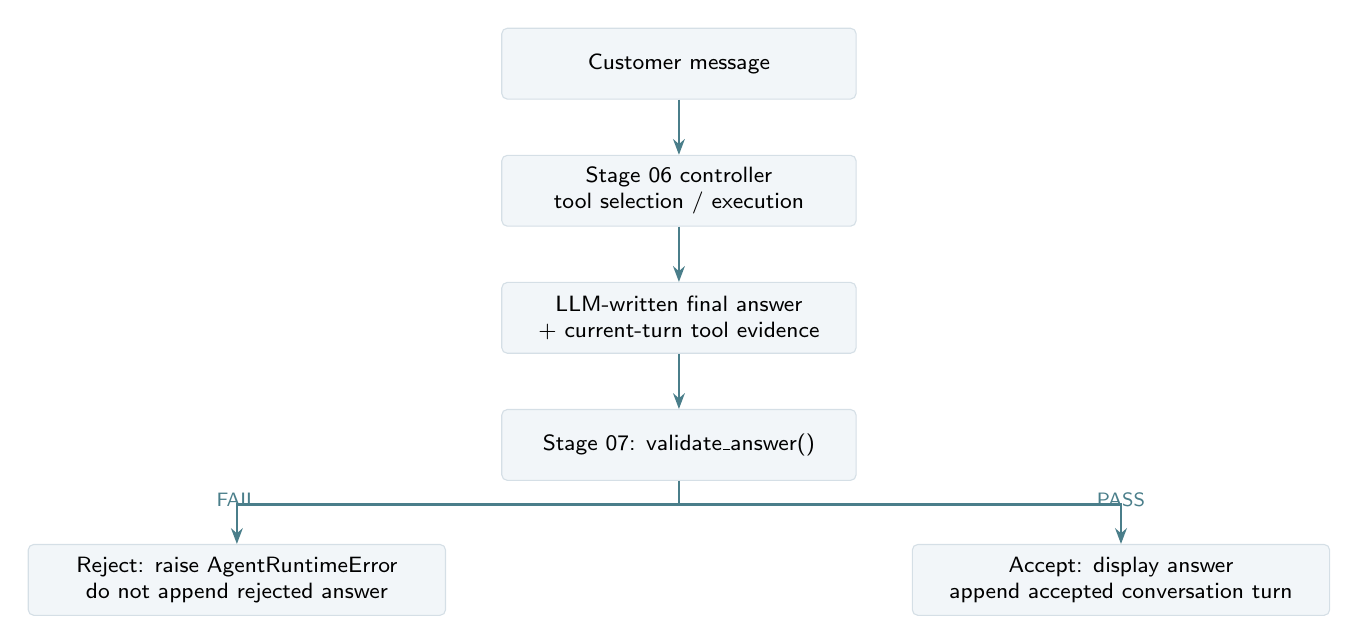
\begin{tikzpicture}[node distance=7mm, every node/.style={font=\sffamily\footnotesize},
 b/.style={draw=Rule,fill=Pale,rounded corners=2pt,align=center,minimum width=45mm,minimum height=9mm},
 arrow/.style={-{Stealth[length=2.0mm]},thick,color=Sea}]
\node[b] (user) {Customer message};
\node[b,below=of user] (ctrl) {Stage 06 controller\\tool selection / execution};
\node[b,below=of ctrl] (llm) {LLM-written final answer\\+ current-turn tool evidence};
\node[b,below=of llm] (guard) {Stage 07: validate\_answer()};
\node[b,below left=8mm and 7mm of guard,minimum width=53mm] (reject) {Reject: raise AgentRuntimeError\\do not append rejected answer};
\node[b,below right=8mm and 7mm of guard,minimum width=53mm] (accept) {Accept: display answer\\append accepted conversation turn};
\draw[arrow] (user)--(ctrl); \draw[arrow] (ctrl)--(llm); \draw[arrow] (llm)--(guard);
\draw[arrow] (guard.south) -- ++(0,-3mm) -| node[pos=0.65,above]{\scriptsize FAIL} (reject.north);
\draw[arrow] (guard.south) -- ++(0,-3mm) -| node[pos=0.65,above]{\scriptsize PASS} (accept.north);
\end{tikzpicture}
\end{center}

\textbf{Fail-closed behavior.} A rejected answer raises a controlled \code{AgentRuntimeError} listing issue codes and is not appended as a successful assistant response. The two controller-level tests were designed to verify both sides: blocking an invalid answer without polluting history and permitting a supported answer. \textbf{Important limitation:} the guard presently rejects; it does not automatically regenerate a corrected response. A live rejection therefore requires inspection and, if appropriate, better retrieval or prompt instructions.

\subsection{07.7 --- Citation verification: where a reference comes from matters}
The validator accepts \emph{current-turn} tool payloads with tool names and structured outputs. For product references, it constructs a set of observed \code{(source_id, page)} pairs from \code{search_product_brochures} results. The final answer's explicit citation patterns, such as \code{filter-optimizer, p.2}, must resolve to one of those retrieved pairs. A brochure file that exists in the corpus but was not returned in that turn is not silently considered supporting evidence.

For service references, it collects the report IDs exposed by \code{compare_service_costs}: task analogs, the best historical analog and regional historical rate comparators. References such as \code{FSR-0027} must appear in that evidence set. A fabricated ID such as \code{FSR-9999} is rejected with a citation error.

\begin{warnbox}
\textbf{Reference existence is not semantic entailment.} The successful validation of \code{filter-optimizer, p.2} means the cited page was returned by the authorized retrieval tool. It does not mean that the page proves a given diagnosis or a guaranteed performance outcome. Claims about physical causes, model suitability and compatibility still require direct scrutiny of source wording, ideally including the original brochure PDF when needed.
\end{warnbox}

\subsection{07.8 --- Monetary checks, currencies and site-specific uncertainty}
The cost validator collects permitted numeric amounts \emph{per currency} from the output of the deterministic estimator. These include recorded line totals, relevant unit rates, the historical reconstructed amount, explicitly reported totals from selected precedents and appropriate local historical hourly rates. It also allows the single transparent deduction modeled for customer-supplied cloths when the source contains an identifiable cloth component.

For the mandatory Chile case, the controlling historical comparison is:
\[
 303.80 + 655.20 + 1{,}176.00 + 62.40 + 18.00
 = \boxed{2{,}215.40\ \mathrm{EUR}}.
\]
When the customer supplies twelve replacement cloths, the observed EUR~1,176.00 cloth-purchase line can be removed from that \emph{historical planning comparison}, yielding:
\[
 2{,}215.40 - 1{,}176.00 = \boxed{1{,}039.40\ \mathrm{EUR}}.
\]
These results are not a new invoice, approved tariff or Chilean quote. The first is reconstructed from a truncated Swedish report, \code{FSR-0027}; the second is an explicitly qualified arithmetic scenario excluding a historical part-purchase line. The estimator's Chile \code{site_specific_budget} remains unavailable without adequate evidence.

The guard checks explicit amounts with currency identifiers (for example, \code{2215.40 EUR}) as well as amounts preceded by the euro sign. It rejects unsupported monetary figures and selected syntactic cases of mixed-currency addition. It blocks affirmative wording claiming a confirmed/final Chilean quote when the tool payload reports no site-specific budget. The code permits narrowly labeled approximate integer rounding within fifty euro cents of a supported number; that behavior should not be mistaken for free permission to round other numbers.

\textbf{What this accomplishes.} The LLM may explain a calculation, but it cannot freely substitute a convincing new rate or invent a current price without risking rejection. \textbf{What it does not accomplish.} The implementation does not parse every possible mathematical expression, currency symbol or linguistic paraphrase; it does not authorize exchange rates or infer current VAT, travel origin or labor tariffs.

\subsection{07.9 --- Additional guard checks and the exact limitations of a pattern-based gate}
Other rules reject empty answers, malformed tool outputs, tool failures and some unsupported quantified performance guarantees. The latter is motivated by an adversarial request such as ``Can you guarantee 50\% cost savings if we install Filter Optimizer?'' A confident model response cannot transform that request into brochure evidence that does not exist.

\begin{longtable}{@{}L{44mm}L{55mm}L{46mm}@{}}
\toprule
\textbf{Guarded category} & \textbf{Example unsafe behavior} & \textbf{Expected check}\\\midrule\endfirsthead
\toprule\textbf{Category} & \textbf{Illustrative violation} & \textbf{Check}\\\midrule\endhead
Brochure citation & Page 99 cited when page 99 was not retrieved. & Reject unknown brochure/page pair.\\
Service citation & Invented \code{FSR-9999}. & Reject non-retrieved report ID.\\
Monetary provenance & Claim of unsupported \code{9999 EUR}. & Reject ungrounded currency amount.\\
Currencies & \code{300 EUR + 500 USD}. & Reject detected cross-currency addition.\\
Quote boundary & ``Confirmed Chile quote'' with a null site budget. & Reject designated definitive pricing language.\\
Performance guarantee & Unsupported quantitative improvement guarantee. & Reject targeted guarantee pattern.\\
Tool integrity & Empty answer or tool execution error. & Reject or surface controlled error.\\
\bottomrule
\end{longtable}

\textbf{Known blind spots must be disclosed.} Regular expressions cannot prove that a real page entails an industrial claim. Alternative currency notations, unrecognized arithmetic syntax and subtle implied guarantees may evade matching. Legitimate complex responses can also encounter false positives. The current code provides narrow prompt-injection resistance through tool boundaries, but the evidence supplied here does \emph{not} establish a comprehensive prompt-injection security evaluation. A complete semantic critic, automatic retry strategy and independent engineering sign-off were not implemented or verified in this recorded stage.

\subsection{07.10 --- The sixteen targeted tests: what each one demonstrates}
After the patch, Windows PowerShell reported \textbf{16 collected tests and 16 passed} in \textbf{3.61 seconds}; the targeted suite was repeated and again reported \textbf{16 passed}, in \textbf{3.58 seconds}. The actual test names and their intended coverage are summarized below.

\begin{longtable}{@{}L{8mm}L{68mm}L{69mm}@{}}
\toprule
\textbf{No.} & \textbf{Actual test} & \textbf{Validation concern}\\\midrule\endfirsthead
\toprule\textbf{No.} & \textbf{Test} & \textbf{Concern}\\\midrule\endhead
1 & \path{test_valid_brochure_citation} & A retrieved, real brochure/page is accepted.\\
2 & \path{test_made_up_brochure_page_fails} & A fabricated page for a known brochure is rejected.\\
3 & \path{test_made_up_brochure_fails} & An unknown brochure source is rejected.\\
4 & \path{test_grounded_report_citation} & A report ID returned by the cost tool is permitted.\\
5 & \path{test_nonexistent_report_citation_fails} & A nonexistent service-report ID is rejected.\\
6 & \path{test_unsupported_price_fails} & An invented price unsupported by tool evidence is rejected.\\
7 & \path{test_supported_components_and_derived_minus_cloth} & Supported cost components and the explicit cloth deduction are accepted.\\
8 & \path{test_mixed_currency_arithmetic_fails} & A detected mixed-currency sum is rejected.\\
9 & \path{test_confirmed_site_quote_fails} & A definitive site quote is rejected without a site budget.\\
10 & \path{test_guaranteed_savings_without_evidence_fails} & An unsupported quantitative guarantee is rejected.\\
11 & \path{test_euro_symbol_amount_is_grounded} & A supported euro-sign amount is accepted.\\
12 & \path{test_invented_euro_symbol_amount_rejected} & An unsupported euro-sign amount is rejected.\\
13 & \path{test_empty_output_rejected} & A blank model response is invalid.\\
14 & \path{test_missing_evidence_rejects_money} & A monetary statement without supporting evidence is rejected.\\
15 & \path{test_controller_enforcement_prevents_history_pollution} & Guard failure does not commit invalid response to history.\\
16 & \path{test_controller_enforcement_permits_supported_answer} & Guard permits a grounded controller response.\\
\bottomrule
\end{longtable}

All sixteen tests are offline/synthetic acceptance examples. They establish the specified cases under controlled test fixtures; they do not establish population-level routing accuracy, complete semantic citation support, or robustness to every adversarial phrasing.

\subsection{07.11 --- Whole-project regression: successful integration without earlier-stage breakage}
The user subsequently executed the full project suite. The terminal returned \textbf{79 passed in 4.12 seconds} and, on a repeated run, \textbf{79 passed in 4.13 seconds}. The combined inventory is:
\begin{tabularx}{\textwidth}{@{}Y r@{}}
\toprule
\textbf{Test family} & \textbf{Passed}\\\midrule
Stage 00 CLI smoke test & 1\\
Stage 02 typed evidence schemas & 13\\
Stage 03 brochure retrieval & 7\\
Stage 04 historical service extraction & 12\\
Stage 05 evidence-based cost estimation & 18\\
Stage 06 autonomous controller & 12\\
Stage 07 response guard and integration & 16\\\midrule
\textbf{Total} & \textbf{79 / 79}\\\bottomrule
\end{tabularx}

This progression is an important piece of engineering evidence: the user did not simply ignore an initial failure. Two missing-integration tests first failed, the patch was applied, its constructor flag was visibly present, the sixteen targeted tests passed, and the full cross-stage suite passed twice. It demonstrates both the intended new behavior and the absence of regressions \emph{among the tested cases}.

\subsection{07.12 --- Reverify the local dependencies without spending API credits}
The user also ran:
\begin{examplebox}
\footnotesize\ttfamily
.\textbackslash.venv\textbackslash Scripts\textbackslash python.exe -m\newline
\hspace*{2em}metso\_agent.agent.chat --check-local
\end{examplebox}
The check returned:
\begin{examplebox}
\footnotesize\ttfamily
Checking local-only dependencies (no network calls)...\\
Product retrieval usable: True\\
Service ledger readable: 50 reports\\
Check completed without external API calls.
\end{examplebox}

The conclusion is narrowly scoped: after the patch, both local evidence resources were reachable and the no-network smoke check still worked. This does \emph{not} prove that the external LLM model will produce an acceptable answer when the new guard is enabled; that requires a separate observed live run.

\subsection{07.13 --- What remains unverified in the supplied execution transcript}
An accurate sign-off must separate success from outstanding requirements. At the end of the supplied Stage 07 transcript, the following work was \emph{not demonstrated}:
\begin{enumerate}
\item \textbf{Live guarded execution.} Re-run the two mandatory Metso prompts under the updated interactive CLI. Record selected tool names and whether the response is accepted or blocked. In particular, the first Larox answer must not assert an unproven physical cause, and the second must keep a reconstructed Swedish EUR historical amount separate from any unsupported Chile quote.
\item \textbf{Adversarial live trials.} Try an unsupported 50\% savings guarantee, an invented Chile quotation, a nonexistent FSR reference, and mixed-currency arithmetic. Confirm that the response is either already cautious or the guard refuses it. An uncaught or unjustified rejection should be documented as a defect.
\item \textbf{Human evidence review.} Compare consequential brochure claims with original pages, and reconcile cost facts against source lines in \code{FSR-0027} and selected Chile reports. Prior snapshots of \path{docs/private/stage04_gold_review.md} showed pending decisions; the present log does not show those decisions completed.
\item \textbf{Prompt-injection and fresh-session evaluation.} Test a synthetic hostile instruction embedded in a retrieved passage and a clean-session clarification sequence. The existing sixteen tests do not by themselves establish comprehensive security or independent cold-start behavior.
\item \textbf{Release safety.} Verify the exact staged Git files, any prior commits, public documentation, archived PDFs/TeX and private cache/secret exclusions. The current transcript does not independently establish a publishable Git history.
\end{enumerate}

A manual source-validation sheet should record: \emph{case ID, customer prompt, selected tool(s), exact claim, retrieved file/page or FSR/line, whether the source actually entails the claim, numerical check, guard decision, reviewer notes and correction}. Test results should be reproducible without copying private raw data into the public code repository.

\subsection{07.14 --- Exact commands for the final acceptance gate}
From the project's existing Windows PowerShell prompt, the validated commands are:
\begin{examplebox}
\small\ttfamily
.\textbackslash.venv\textbackslash Scripts\textbackslash python.exe -m pytest\newline
\hspace*{2em}tests/test\_response\_guard.py -v\\[2pt]
.\textbackslash.venv\textbackslash Scripts\textbackslash python.exe -m pytest -q\\[2pt]
.\textbackslash.venv\textbackslash Scripts\textbackslash python.exe -m\newline
\hspace*{2em}metso\_agent.agent.chat --check-local
\end{examplebox}
These commands already passed in the reported Windows session. The \emph{remaining} executable acceptance action is a guarded live run:
\begin{examplebox}
\small\ttfamily
.\textbackslash.venv\textbackslash Scripts\textbackslash python.exe -m\newline
\hspace*{2em}metso\_agent.agent.chat --allow-external-evidence\newline
\hspace*{2em}--verbose
\end{examplebox}
The original two mandatory prompts must then be entered verbatim, starting from an ordinary new chat session. If a response is blocked by \code{Evidence guard rejected response}, record the issue code and the responsible sentence; do not disable the guard merely to make a demonstration look successful. Correct the source selection, overly broad system instructions or output formatting, then repeat the targeted regression suite.

The source-publication commands should be repeated separately before any \code{git add} or public push: \code{git status --short --ignored}, \code{git ls-files}, and \code{git check-ignore -v} on \code{.env}, \code{raw/}, \code{local_cache/}, \path{docs/private/} and any private study-book artifacts. A successful Python test result says nothing about whether \code{git add .} would include an unignored report PDF.

\subsection{07.15 --- Stage 07 acceptance matrix and defensible status}
\begin{longtable}{@{}L{53mm}L{56mm}L{36mm}@{}}
\toprule
\textbf{Requirement} & \textbf{Evidence in the Windows log} & \textbf{Status}\\\midrule\endfirsthead
\toprule\textbf{Requirement} & \textbf{Observed support} & \textbf{Status}\\\midrule\endhead
Validation source files available & Targeted suite imports and executes all new tests. & \textbf{Verified}\\
Controller patch applied & Both files patched; backup path reported. & \textbf{Verified}\\
Guard constructor present & Three matching code locations returned. & \textbf{Verified}\\
Initial test failure diagnosed & 77 passed, 2 failed before integration. & \textbf{Explained}\\
Targeted guard tests & 16/16 passed twice. & \textbf{Verified}\\
Entire regression suite & 79/79 passed twice. & \textbf{Verified}\\
Local brochure and FSR tools & Retrieval usable; 50 reports readable. & \textbf{Verified}\\
Live response gate accepts both demonstrations & No post-patch live trace supplied. & \textbf{Pending}\\
Human technical claim/source checks & No completed signed review shown. & \textbf{Pending}\\
General semantic entailment and injection resistance & Not covered comprehensively by current patterns. & \textbf{Limited}\\
Public repository confidentiality & No final staged/history audit in this log. & \textbf{Pending}\\
Public video and Recright submission & Not evidenced in current transcript. & \textbf{Pending}\\
\bottomrule
\end{longtable}

\begin{keybox}
\textbf{Stage 07 engineering judgment: automatic integration and regression testing PASS; final live/manual sign-off remains OPEN.} The user's actual Windows log confirms the evidence-guard patch, two independent passes of the sixteen new targeted tests, two full successful 79-test runs, and a successful local-source check. The implementation is a meaningful and tested boundary against several common citation and monetary hallucinations. It is \emph{not} a complete proof of factual correctness, does not automatically issue commercial quotations, and has not yet been demonstrated in a fresh live session after activation.
\end{keybox}

\subsection{07.16 --- Lessons learned and priorities before the employer deadline}
This stage illustrates why testing both \emph{the validator itself} and \emph{its placement inside the agent} matters. A component can pass fourteen logic tests while its two controller-level checks fail because the integration has not been installed. The progression from \emph{77 passed / 2 failed} to \emph{79 passed / 0 failed} is the strongest directly observed integration result. The intervention also preserves the useful Stage 06 implementation rather than replacing it wholesale.

The next priority is not another large subsystem. It is to run the two official prompts under the guarded CLI; correct any false positive or unsupported output; make a brief human check of high-risk source claims; and freeze a clean, reproducible public code package. Metso's required deliverables also include a publicly accessible 5--7 minute walkthrough and the separate Recright video interview, all due \textbf{20 October 2026 at 23:59 Helsinki local time}. Optional flotation analysis should not displace those mandatory steps.

\vspace{4mm}
\begin{center}
{\sffamily\color{Gray}\footnotesize END OF PART X -- STAGE 07 EVIDENCE AND RESPONSE VALIDATION}\\[2mm]
{\sffamily\bfseries\color{Navy}AG is your G!}
\end{center}


\clearpage
\section{Stage 08 --- Implement optional flotation data analysis}
\label{sec:stage08}
\begin{keybox}
\textbf{Stage 08 decision: IMPLEMENTED AND LIVE-DEMONSTRATED, WITH QUALIFIED LIMITATIONS.}
The candidate's 19 October 2026 Windows transcript establishes that a local flotation analytics module ran on the supplied 4,097-row CSV, twelve dedicated statistical tests passed, a third tool named \code{analyze_flotation} was connected to the conversational controller, the optional prompt was answered through that tool, and the final complete project regression reached \textbf{113 passed / 0 failed}. The last live Chile service-cost question also succeeded after a narrowly scoped evidence-guard correction. Eighteen recurring deprecation warnings and a minor statistical phrasing issue remain; neither should be hidden or conflated with test failure. This is not proof of contractual product quality or commercial quotation readiness.
\end{keybox}

\subsection{08.1 --- The actual question and the purpose of this optional feature}
The Metso assignment includes a third, explicitly optional conversation:
\begin{examplebox}
\textit{``The customer is getting 3.1\% silica and 64.5\% iron in their concentrate. They think that's normal. What do you think?''}
\end{examplebox}
The user is asking whether a reported concentrate composition is \emph{normal}. There are at least two possible meanings: (1) whether similar observations occurred in the available historical record, and (2) whether the composition satisfies the customer's contractual quality limit. The supplied CSV can support the first answer. No provided contract, specification or customer-specific acceptance threshold supports the second.

\textbf{Why build a third tool?} A general-purpose LLM cannot be treated as the authoritative calculator for empirical percentiles and simultaneous conditions across thousands of rows. A small deterministic Python analyzer can produce the counts, summary statistics and data-quality flags directly from source measurements, after which the agent can explain what they mean in conversational terms. This preserves the existing division of responsibility: \emph{the LLM selects and explains; local tools retrieve and compute}. The optional task was explicitly constrained by a 45-minute suggested time box; the design intentionally avoids predictive modeling, new infrastructure, a GUI and causality claims.

\subsection{08.2 --- Starting point: existing agent and safeguards}
When Stage 08 began, the project already included the Stage 03 brochure retriever, Stage 04 service-report parser, Stage 05 historical cost estimator, Stage 06 tool-calling controller, and Stage 07 response guard. The first later recorded local baseline was \textbf{85 passed} following the Stage 07 live-guard hotfix. The guarded CLI could already use \code{search_product_brochures} and \code{compare_service_costs}; \code{--check-local} could access product retrieval and all 50 historical service reports without an external API call.

The new feature needed to be \emph{additive}. The source CSV was required to remain inside \path{raw/data/}; source files, generated data outputs, API secrets and private review worksheets must not be published. The previous Stage 07 validator also had to remain attached to the agent. Accordingly, the analytics module and its tests were added before the optional integration patch was run, and the patch reported a local backup rather than deleting earlier modules.

\subsection{08.3 --- Concrete implementation artifacts and responsibilities}
\begin{tabularx}{\textwidth}{@{}L{59mm}Y@{}}
\toprule
\textbf{Path or component} & \textbf{Role in the observed implementation}\\\midrule
\path{src/metso_agent/analytics/flotation.py} & Reads historical measurements; checks inputs and schema; calculates statistics, threshold frequencies and time gaps; offers a standalone CLI and structured output.\\
\path{src/metso_agent/analytics/__init__.py} & Makes the analytics directory an importable Python package.\\
\path{tests/test_flotation.py} & Twelve dedicated tests of numerical, validation, missing-input and data-quality behavior.\\
\path{tests/test_flotation_agent_optional.py} & Four agent-facing tests of the optional tool's dispatch and use, as represented in the later 101-test suite.\\
\path{scripts/apply_stage08_tool.py} & Installs the third tool into the existing agent structure; the run patched \path{tools.py} and \path{controller.py}.\\
\path{docs/flotation_analysis.md} & Standalone explanatory documentation for the method and its boundaries.\\
\path{docs/private/stage07_manual_validation.md} & Private, Git-ignored manual source-review checklist carried forward from Stage 07; not evidence that review decisions are complete.\\
\path{local_cache/stage08_flotation_result.json} & User-selected private destination for machine-readable output; the command ran and printed the structured result.\\
\bottomrule
\end{tabularx}

\textbf{Source of truth.} The filename used during computation was \code{flotation_process_data_hourly.csv}. Every historical statistic below comes from the observed executable output, not from guessing an ore-quality standard or constructing a fixed response to the demonstration sentence.

\subsection{08.4 --- Dependency and confidentiality checks before adding the tool}
The Windows interpreter was Python \textbf{3.12.4}. The installed numerical libraries were \textbf{pandas 2.3.3} and \textbf{NumPy 2.5.4}; an attempted installation command returned \code{Requirement already satisfied}. The source-file presence check for \path{raw/data/flotation_process_data_hourly.csv} returned \code{True}. Both tests and analytics module files were subsequently confirmed present.

An early invocation of \code{pytest tests/test_flotation.py} reported \textit{file or directory not found}; this was a timing/path-of-copy issue, not a failed test assertion. After the new files were copied into the project, the same command collected twelve items and all twelve passed. One attempt to run the pytest command while the assistant was still at the interactive \code{You >} prompt was interpreted as an ordinary chat question, not a terminal command. The candidate exited the chat with \code{exit}, returned to PowerShell and executed pytest correctly. These events matter because a reproducible procedure must distinguish \emph{shell} from \emph{chat application} and missing-file setup errors from actual software defects.

The command \code{git check-ignore -v docs/private/stage07_manual_validation.md} returned \code{.gitignore:64:docs/private/}, verifying that this private worksheet path was ignored in the reported working tree. This does not by itself establish that the entire repository or its historical commits are safe for publication.

\subsection{08.5 --- Data model, source range and quality profile}
The implemented analyzer reported \textbf{4,097 observations and 24 columns}: one time column and 23 process or quality measurements. Its time metadata covered \textbf{2017-03-10 01:00:00} through \textbf{2017-09-09 23:00:00}. The structured output reported zero duplicated timestamps and one gap longer than one hour; the largest gap was \textbf{319 hours} (13 days and 7 hours). The record is therefore \emph{hourly where present}, not uninterrupted over the calendar period.

The two variables actually needed to answer the customer are \texttt{\% Silica Concentrate} and \texttt{\% Iron Concentrate}. Other process measurements are outside the narrow statistical assessment. A missing or non-numeric quality column produces an explicit rejection in the unit-test cases. No units were invented for unlabelled reagent, air-flow, pulp-level or process variables.

\begin{tabularx}{\textwidth}{@{}Y r r@{}}
\toprule
\textbf{Statistic (from the executed analyzer)} & \textbf{Silica concentrate} & \textbf{Iron concentrate}\\\midrule
Customer measurement & 3.10\% & 64.50\%\\
Historical mean & 2.326754\% & 65.050084\%\\
Median & 2.00\% & 65.21\%\\
Sample standard deviation & 1.124783 & 1.118099\\
First quartile (Q1) & 1.44\% & 64.37\%\\
Third quartile (Q3) & 3.01\% & 65.86\%\\
Minimum & 0.60\% & 62.05\%\\
Maximum & 5.53\% & 68.01\%\\\bottomrule
\end{tabularx}

The customer's silica observation exceeds both the mean and Q3 of silica; the customer's iron observation falls below the mean and median of iron, but above Q1. These are meaningful relative historical positions. They are \emph{not} a verdict that the concentrate meets or violates any particular buyer's contract.

\subsection{08.6 --- The threshold questions that were actually computed}
Let $S_i$ and $F_i$ represent silica and iron percentages in observed hourly row $i$, and let $n=4097$. The program computes the following inclusive comparisons using the observed customer thresholds:
\begin{align}
N_S &= \sum_{i=1}^{4097} \mathbb{1}[S_i \geq 3.1] = 981,\\
N_F &= \sum_{i=1}^{4097} \mathbb{1}[F_i \leq 64.5] = 1142,\\
N_{SF} &= \sum_{i=1}^{4097} \mathbb{1}[S_i \geq 3.1\ \land\ F_i \leq 64.5] = 823.
\end{align}
\begin{tabularx}{\textwidth}{@{}Y r r@{}}
\toprule
\textbf{Observed historical condition} & \textbf{Hourly rows} & \textbf{Share of 4,097 rows}\\\midrule
Silica $\geq 3.1\%$ & 981 & 23.94\%\\
Iron $\leq 64.5\%$ & 1,142 & 27.87\%\\
Both conditions simultaneously & 823 & 20.09\%\\\bottomrule
\end{tabularx}

The important distinction is that \textbf{20.09\% means the empirical share of rows satisfying both inequalities}, not the frequency of an \emph{exact} (3.1, 64.5) pair. It also is not the probability that the customer's concentrate meets specifications or a forecast of future operating states. The implementation computed these statistics on the full observed file; it did not claim independent samples, equal operating modes or continuous chronology.

\subsection{08.7 --- Correlation: useful description, no causal conclusion}
The output reported a Pearson correlation of \textbf{$r=-0.801208$} between the historical iron and silica concentrate measurements. Within this specific dataset, higher silica measurements tended to accompany lower iron measurements. This is a strong negative \emph{association}, but it does not identify a root cause, prove which operating parameter to change, or quantify a product's effect. Both percentages may respond to multiple common plant conditions, process controls or feed properties.

The agent's answer appropriately described the value as historical and warned that correlation is not cause and effect. A future investigation could stratify by feed period, plant state and data gaps, but those follow-on analyses were not implemented or evidenced in the supplied Stage 08 transcript and therefore are not claimed as delivered.

\subsection{08.8 --- Dedicated tests: what the twelve passes establish}
The user executed \code{python -m pytest tests/test_flotation.py -v}. The run collected \textbf{12 items} and returned \textbf{12 passed, 14 warnings in 1.63 seconds}. The tests inspected numerical behavior and input validation rather than relying on a single hand-entered successful prompt:
\begin{longtable}{@{}L{70mm}L{77mm}@{}}
\toprule
\textbf{Observed test name / family} & \textbf{What the pass supports}\\\midrule\endfirsthead
\toprule\textbf{Test or family} & \textbf{Evidence scope}\\\midrule\endhead
\code{test_inclusive_threshold_counts} & The configured $\geq$ and $\leq$ counts work for a fixture.\\
\code{test_source_and_n_are_reported} & Source identity and observation count are returned.\\
\code{test_means_are_computed} & Historical summary values are computed from data.\\
{\footnotesize\path{test_distinct_thresholds_change_counts}} & The analyzer is not hard-coded to the demo percentages.\\
\code{test_reject_missing_csv} & Missing inputs fail explicitly rather than returning invented results.\\
\code{test_reject_invalid_threshold_nan} & Not-a-number thresholds are rejected.\\
\code{test_reject_threshold_boolean} & Boolean values cannot silently become percentage numbers.\\
\code{test_reject_percentage_outside_range} & Percentage thresholds outside the permitted range are rejected.\\
\code{test_reject_missing_quality_column} & Required concentrate fields are enforced.\\
\code{test_reject_non_numeric_measurement} & Unexpected non-numeric quality observations are rejected.\\
\code{test_detect_timestamp_gap} & Broken chronological coverage is surfaced.\\
\code{test_no_contractual_claim} & Output does not equate historical prevalence with contractual acceptance.\\\bottomrule
\end{longtable}

These passes support the specific tested behaviors. They do not replace a live execution, a reviewer inspection of the customer's actual contract, or a statistical study of future generalization.

\subsection{08.9 --- Standalone execution and reproducible observed outputs}
From the project root, the candidate ran the analyzer independently of the LLM:
\begin{examplebox}
\small\ttfamily
.\textbackslash.venv\textbackslash Scripts\textbackslash python.exe -m\newline
\hspace*{1.4em}metso\_agent.analytics.flotation --silica 3.1 --iron 64.5
\end{examplebox}
The terminal printed \code{observations: 4097}, \code{columns: 24}, the three counts (981, 1142, 823), the corresponding percentages (23.94\%, 27.87\%, 20.09\%), correlation $-0.801208$, maximum gap 319.0 hours and a warning that history is not a contractual standard. It also asked for the customer's maximum allowable silica and minimum iron requirements.

Two deliberately different user thresholds confirmed non-fixed computation:
\begin{tabularx}{\textwidth}{@{}Y r r r@{}}
\toprule
\textbf{Input (silica, iron)} & \textbf{Silica $\geq$} & \textbf{Iron $\leq$} & \textbf{Both}\\\midrule
(3.1\%, 64.5\%) & 981 & 1,142 & 823\\
(2.5\%, 65.0\%) & 1,377 & 1,755 & 1,189\\
(4.0\%, 63.5\%) & 475 & 461 & 291\\\bottomrule
\end{tabularx}

The program was also invoked with \code{--json --output} aimed at \path{local_cache/stage08_flotation_result.json}; the displayed JSON included \code{HISTORICAL_DESCRIPTION_ONLY}, structured \code{reference}, \code{counts}, \code{percent_of_rows}, \code{data_quality}, limitations and the customer percentages. Its displayed numbers agree with the text-mode outputs. The transcript does not include a separate post-write file-existence check, so the recorded command and printed data, rather than an independently checked on-disk file, are the established observations.

\subsection{08.10 --- Install the third tool without replacing the first two}
Before the optional patch, the candidate verified both Stage 07 markers in \path{controller.py}: \code{STAGE07_EVIDENCE_GUARD} and \code{STAGE07_LIVE_HOTFIX_V1}. Then the user executed the additive installation script. Its observed output was:
\begin{examplebox}
\footnotesize\ttfamily
Patched: src\textbackslash metso\_agent\textbackslash agent\textbackslash tools.py\\
Patched: src\textbackslash metso\_agent\textbackslash agent\textbackslash controller.py\\
Backups: local\_cache\textbackslash stage08\_backups\textbackslash 20261019T131110Z
\end{examplebox}

This indicates that the existing controller was modified to recognize \code{analyze_flotation} and the corresponding adapter rather than exchanging the whole project for a new program. The revised runtime had three distinct evidence destinations:
\begin{center}
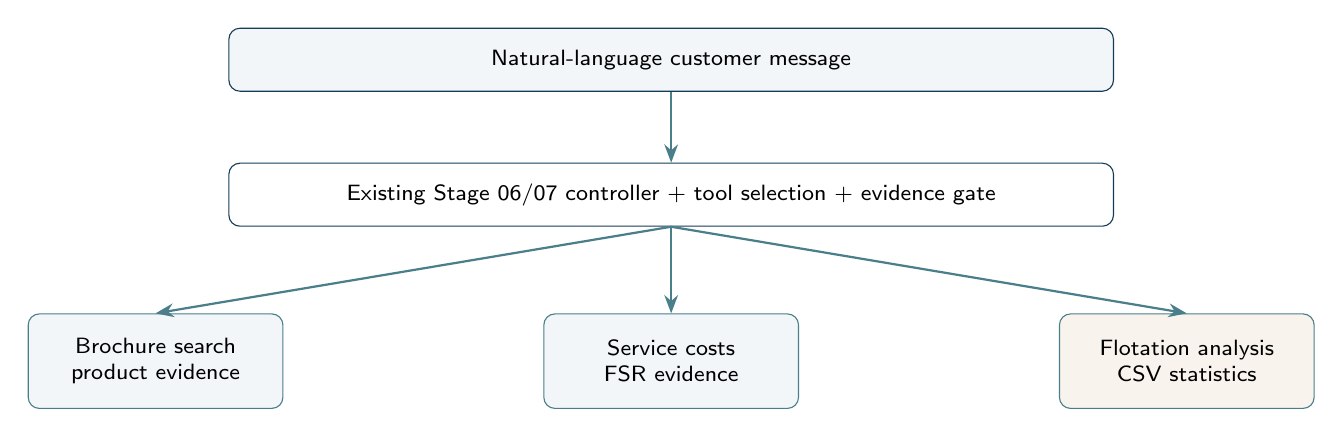
\begin{tikzpicture}[node distance=9mm and 6mm, every node/.style={font=\sffamily\footnotesize,align=center},>=Stealth]
\node[draw=Navy,rounded corners,fill=Pale,text width=11cm,minimum height=8mm] (msg) {Natural-language customer message};
\node[below=of msg,draw=Navy,rounded corners,fill=white,text width=11cm,minimum height=8mm] (agent) {Existing Stage 06/07 controller + tool selection + evidence gate};
\node[below left=11mm and -7mm of agent,draw=Sea,rounded corners,fill=Pale,text width=3.0cm,minimum height=12mm] (a) {Brochure search\\product evidence};
\node[below=11mm of agent,draw=Sea,rounded corners,fill=Pale,text width=3.0cm,minimum height=12mm] (b) {Service costs\\FSR evidence};
\node[below right=11mm and -7mm of agent,draw=Sea,rounded corners,fill=Gold!10,text width=3.0cm,minimum height=12mm] (c) {Flotation analysis\\CSV statistics};
\draw[->,thick,Sea] (msg)--(agent);
\draw[->,thick,Sea] (agent.south) -- (a.north);
\draw[->,thick,Sea] (agent.south) -- (b.north);
\draw[->,thick,Sea] (agent.south) -- (c.north);
\end{tikzpicture}
\end{center}

\subsection{08.11 --- Whole-project regression grew from 85 to 101 tests}
After adding the optional-tool integration, the candidate ran the entire project suite. The terminal returned \textbf{101 passed, 18 warnings in 4.22 seconds}. Relative to the preceding 85-test baseline, the new feature therefore added \textbf{16 tests}: 12 independent flotation tests and 4 adapter/controller integration tests. The accompanying offline check reported \code{Product retrieval usable: True}, \code{Service ledger readable: 50 reports} and completion without external API calls.

This demonstrates that the three-tool extension did not cause an \emph{observed} regression across the test cases included in the existing suites. It is not a proof that every LLM output is reliable. Accordingly, the next actions in the log exercised all three user intents through the live OpenAI-connected CLI.

\subsection{08.12 --- Live optional-prompt execution: the principal acceptance result}
In the new conversational session, the candidate entered the exact optional Metso wording. The tool trace returned:
\begin{examplebox}
\footnotesize\ttfamily
Tools used: analyze\_flotation
\end{examplebox}
The agent then explicitly cited \code{flotation_process_data_hourly.csv} and 4,097 historical rows; gave silica mean 2.3268\%, median 2.00\%, Q3 3.01\%; iron mean 65.0501\%, median 65.21\%, Q1 64.37\%; the exact count trio 981 / 1,142 / 823; the associated percentages 23.94\% / 27.87\% / 20.09\%; and the negative Pearson association of approximately $-0.8012$. It concluded that the reported composition was less favorable than the historical center and asked for the contract's maximum silica and minimum iron targets before judging acceptability.

\begin{keybox}
\textbf{Optional scenario: LIVE PASS, with a wording refinement.} Tool selection, source provenance, computed numbers and uncertainty are supported by the actual terminal trace. One sentence in the conversational output described the \emph{``exact pair''} as seen in approximately 20\% of hours. That wording is statistically imprecise: \textbf{the computation counted a joint threshold region}, $S \geq 3.1$ and $F \leq 64.5$, not exact equality. This should be corrected in a later prompt template, output validation rule or final demonstration phrasing. The numerical calculation itself is not thereby invalidated.
\end{keybox}

\subsection{08.13 --- Live regression of the mandatory Larox product scenario}
After the flotation answer, the user entered the first mandatory prompt concerning Larox pressure filters and changing feed grade. The agent trace showed \code{Tools used: search_product_brochures}; it located Filter Optimizer evidence on page 2 together with Larox PF/PF-DS supporting pages. The answer discussed recipe sensitivity, cycle control, cloth selection and data collection, and asked for the exact installed model and details of the feed change. It distinguished recommendations from a site-specific guarantee.

\textbf{Quality caution.} Certain phrases about why the filter performance drops can sound more causal than the customer's sparse facts warrant. The text correctly cites documentation about variability but does not establish which physical mechanism is active at that customer's plant. A precise future answer should use \emph{possible contributors to investigate}, not a confirmed diagnosis; mechanical settings or retrofit compatibility should remain subject to site-specific engineering review.

\subsection{08.14 --- Live regression of the Chile service-cost scenario and guard false positive}
The second mandatory question was also re-tried after Stage 08 integration. On the first attempt, the trace showed \code{Tools attempted: compare_service_costs} followed by \code{UNSUPPORTED_SITE_SPECIFIC_QUOTE}. This is a \emph{safe refusal to publish}, not a passing response. The rejected draft was not visible, so the terminal alone cannot prove whether a genuine unsupported quote or a false-positive phrase triggered the block.

A separate narrow investigation found that some \emph{negative} disclaimers about a Chile quotation could be interpreted by the rule-based validator as positive quotation claims. The candidate installed the provided quote-guard correction. The resulting observed patch message named \path{src/metso_agent/validation/response_guard.py} and a private backup under \path{local_cache/stage08_backups/}. Twelve targeted tests then passed, including legitimate negated wording, explicitly affirmative quote statements, a mixed negative-then-positive sentence, unsupported monetary amounts and a supported historical analog.

The entire project suite subsequently reported \textbf{113 passed, 18 warnings in 3.81 seconds}. The normal no-network check still found product retrieval and all fifty historical reports. The candidate then restarted the live Agent and asked the Chile question again: \code{Tools used: compare_service_costs} and a substantive accepted answer were displayed. This supports the operational success of the final correction in that run; it does not reveal the exact wording of the previously blocked model draft.

\subsection{08.15 --- What the final accepted Chile answer did correctly}
The final accepted response did \emph{not} invent a Chile site-specific price. It identified \code{FSR-0027} as a 12-cloth Larox PF-DS activity analog from Sweden, explicitly marked the \textbf{2,215.40 EUR} figure as \code{PROVISIONAL_COMPONENT_SUM_NOT_SOURCE_TOTAL}, showed each historical component and cited report lines. The five visible amounts were:
\begin{tabularx}{\textwidth}{@{}Y r@{}}
\toprule
\textbf{Reconstructed historical component} & \textbf{EUR}\\\midrule
Travel: 4.9 at 62.00 & 303.80\\
Labour: 8.4 at 78.00 & 655.20\\
Twelve cloths at 98.00 & 1,176.00\\
Twenty-four fastening clips at 2.60 & 62.40\\
Cleaning supplies & 18.00\\\midrule
\textbf{Provisional sum of visible components} & \textbf{2,215.40}\\\bottomrule
\end{tabularx}
The response also separated CAD 4,367.00 (\code{FSR-0014}), EUR 2,580.44 (\code{FSR-0031}) and bundled SEK 19,850 (\code{FSR-0044}) rather than combining their currencies. It described the missing technician origin, accommodations, travel and Chilean expenses, and asked for the exact site and who supplies cloths. This is an appropriate \emph{evidence-based historical comparison}, not an approved commercial quote. The physical meaning of the twelve ``cloths'' versus the endless-cloth PF-DS brochure terminology still requires source verification before a real transaction.

\subsection{08.16 --- Remaining technical warnings, risks and unverified gates}
The last complete pytest output was \textbf{113 passed, 18 warnings}. The warnings referenced \path{src/metso_agent/analytics/flotation.py}, especially the pandas/NumPy timedelta comparisons and divisions on lines 96--97, and stated that generic NumPy timedelta units are deprecated. This was nonfatal in the observed environment but is a legitimate future-compatibility defect to address in a dedicated small change. The safe response is to retain passing behavior and explicitly normalize time deltas to a supported unit during a later maintenance pass, then rerun the affected tests; suppressing all warnings is not a durable fix.

\begin{longtable}{@{}L{52mm}L{60mm}L{32mm}@{}}
\toprule
\textbf{Gate or concern} & \textbf{Evidence in the latest logs} & \textbf{Decision}\\\midrule\endfirsthead
\toprule\textbf{Gate} & \textbf{Observed support} & \textbf{Decision}\\\midrule\endhead
Standalone flotation computation & CSV analysis run; three threshold inputs. & \textbf{PASS}\\
Unit tests for statistics & 12/12 passed. & \textbf{PASS}\\
Third-tool integration & Patch successful; 4 agent-facing tests added. & \textbf{PASS}\\
Full-project regression & 101/101, then 113/113 passed. & \textbf{PASS}\\
Live optional prompt & \code{analyze_flotation} used; computed numbers match. & \textbf{PASS}\\
Post-integration Larox prompt & Brochure search used; relevant grounded explanation. & \textbf{PASS}\\
Final post-fix Chile prompt & Cost search used; cautious analog accepted. & \textbf{PASS}\\
Time-series continuity & 319-hour discontinuity disclosed. & \textbf{DISCLOSED}\\
Contract-specific quality verdict & No contract quality limits supplied. & \textbf{NOT CLAIMED}\\
Statistical ``exact pair'' phrase & Wording does not match threshold definition. & \textbf{IMPROVE}\\
NumPy timedelta warnings & 18 deprecation warnings in final suite. & \textbf{NONFATAL}\\
Final human source sign-off & No completed review decision set shown. & \textbf{PENDING}\\
Final Git and public link audit & Not established by this console transcript. & \textbf{PENDING}\\
Video and Recright completion & Not shown in the provided log. & \textbf{PENDING}\\\bottomrule
\end{longtable}

A subtle but important sequence qualification: the optional-prompt and Larox live successes were shown \emph{before} the last quote-guard correction; the final live transcript after the correction shows the Chile cost success, plus 113 passing automated tests. The provided material does not show a \emph{single} subsequent three-question live run after that final fix. This does not negate the separate observed passes but should be noted for a reproducible video demonstration.

\subsection{08.17 --- Suggested final recheck commands and publication boundary}
The following minimal commands reproduce the numerical tests and local state from the candidate's Windows project root:
\begin{examplebox}
\footnotesize\ttfamily
.\textbackslash.venv\textbackslash Scripts\textbackslash python.exe -m pytest -q\\[2pt]
.\textbackslash.venv\textbackslash Scripts\textbackslash python.exe -m\newline
\hspace*{1.5em}metso\_agent.analytics.flotation --silica 3.1 --iron 64.5\\[2pt]
.\textbackslash.venv\textbackslash Scripts\textbackslash python.exe -m\newline
\hspace*{1.5em}metso\_agent.agent.chat --check-local\\[2pt]
.\textbackslash.venv\textbackslash Scripts\textbackslash python.exe -m\newline
\hspace*{1.5em}metso\_agent.agent.chat --allow-external-evidence --verbose
\end{examplebox}

The public code must \emph{not} include \path{raw/}, the employer's supplied \path{data/}, private JSON output, \path{local_cache/}, \code{.env}, API keys, detailed private review notes or this internal full study book. \code{git check-ignore} on the manual-review file is necessary but not sufficient. Before publication, inspect \code{git ls-files}, \code{git status --short --ignored}, any existing commit history and the exact staged paths. The report is a private learning artifact, not one of the required public deliverables.

\subsection{08.18 --- Stage 08 conclusion and priority after acceptance}
\begin{keybox}
\textbf{Final technical conclusion.} Stage 08's optional flotation-analysis capability has been \textbf{successfully implemented and demonstrated}. The system uses a third autonomously selected tool to calculate historical quality statistics from the supplied CSV and communicates the essential uncertainty: silica 3.1\% is above the historical mean, iron 64.5\% is below it, and \textbf{823 of 4,097 hourly observations (20.09\%)} satisfy both adverse-direction threshold conditions. That does not establish that the customer's concentrate is commercially acceptable. The final whole-project regression stands at \textbf{113/113 passing tests}; the evidence-guard fix also permitted the mandatory Chile question to complete with a traceable provisional historical amount rather than an invented binding quote.
\end{keybox}

\textbf{What I learned.} Deterministic, source-aware tools keep numerical claims reproducible and evidence domains separate. Tests must cover both \emph{correct acceptance} and \emph{correct rejection}: overbroad negation rules can create false positives. The 319-hour gap, missing customer contract and noncausal correlation remain part of the honest answer.

\textbf{Next priority.} Freeze Stage 08 except for material defects. Confirm high-risk sources, improve the ``exact pair'' sentence when practical, and prioritize final evaluation, safe public code, a 5--7 minute walkthrough and Recright. Deadline: \textbf{20 October 2026, 23:59 Helsinki local time}.

\vspace{1mm}
\begin{center}
{\sffamily\color{Gray}\footnotesize END OF PART XI -- STAGE 08 OPTIONAL FLOTATION ANALYSIS}\\[2mm]
{\sffamily\bfseries\color{Navy}AG is your G!}
\end{center}

\clearpage
\section{Stage 09 --- Create a genuine evaluation and regression-test suite}
\label{sec:stage09}
\begin{keybox}
\textbf{Technical sign-off: COMPLETE FOR THE OBSERVED STAGE 09 EVALUATION SUITE.}
The candidate's final Windows PowerShell run on 19 October 2026 shows \textbf{147 of 147 automated tests passing}, an offline product-retrieval benchmark previously reporting \textbf{12/12 labeled queries found in the top five} (macro source recall@5 and hit@5 of 100\% on that particular set), and a later, directly recorded \textbf{nine-turn live evaluation with nine correct tool routes and nine completed responses}. Those nine turns represent \textbf{seven distinct labeled scenarios}, because the mixed-intent scenario and the unsupported-guarantee scenario were each repeated. The result establishes a functioning evaluation and reliability checkpoint, \emph{not} a proven 100\% generalization rate or an unconditional public-release approval.
\end{keybox}

\subsection{09.1 --- Why I needed an evaluation stage after building the agent}
Stages 03--08 had produced functioning subsystems: page-aware brochure retrieval, extraction of fifty historical service reports, conservative monetary comparisons, a tool-calling conversation controller, response validation, and an optional flotation analysis tool. Passing individual component tests was necessary but insufficient. The employer's task is ultimately a \emph{conversational} one: the model must choose the right evidence source, use that evidence correctly, ask useful clarifying questions, and refrain from invented facts. A single successful screenshot of each mandatory prompt cannot establish these properties under variation.

I therefore added Stage 09 to convert an informal demonstration into a repeatable set of observations. It addresses four related but separate questions: (1) does retrieval find the expected brochure? (2) does the controller select the appropriate tool or set of tools? (3) does a response actually reach the user instead of failing after tool selection? and (4) is the published answer substantively supported and safe? The first three can be partly automated; the fourth requires human review because simple pattern checks cannot prove the truth of every natural-language claim.

\subsection{09.2 --- What was built and where it lives}
The Stage 09 evaluation package added a separate metrics module, evaluation runner, labeled scenarios, tests and private review guidance. A later reliability patch modified the existing controller, response guard and chat entry point \emph{in place after creating private backups}; it did not replace the brochure search, historical service ledger, or flotation calculator.

\begin{longtable}{@{}L{58mm}L{101mm}@{}}
\toprule
\textbf{Artifact} & \textbf{Purpose and disclosure policy}\\\midrule\endfirsthead
\toprule\textbf{Artifact} & \textbf{Purpose}\\\midrule\endhead
\path{src/metso_agent/evaluation/metrics.py} & Label matching, transcript parsing and summary metrics. Code may be distributed after source review.\\
\path{scripts/run_stage09_eval.py} & Runs retrieval and transcript evaluations and writes sanitized result summaries.\\
\path{tests/test_stage09_evaluation.py} & Seventeen unit tests for benchmark parsing, scoring, duplicate/error handling and sanitized output.\\
\path{docs/private/stage09_gold_cases.jsonl} & Private labeled benchmark of 33 evaluation cases; includes expected routes and twelve product retrieval labels. Do not publish this file without explicit permission.\\
\path{docs/private/stage09_manual_review.md} & Human evaluation worksheet for claims, citations, scope and safety. Private.\\
\path{docs/evaluation_stage09.md} & Evaluation-method description, potentially public after source-text review.\\
\path{scripts/apply_stage09_reliability_fix.py} & Checked, backup-producing reliability patch installer.\\
\path{tests/test_stage09_reliability_fix.py} & Seventeen additional tests for negative guarantees, guarded fallback responses and private session logging.\\
\path{local_cache/stage09_after_fix_run1.txt} & Actual post-fix interactive transcript produced by the agent; private and ignored by Git.\\
\path{local_cache/stage09_after_fix_results.json} & Sanitized scoring summary from the recorded run; retain as private test evidence.\\\bottomrule
\end{longtable}
\textbf{Design rationale.} I kept metrics and test fixtures out of the controller's runtime decision logic, because a scoring benchmark must not become a hidden lookup table for answering the demonstration prompts. The evaluator observes the agent; the normal agent continues to call its three evidence tools. The labels form a test contract, not a universal definition of what constitutes safe human behavior in every adversarial prompt.

\subsection{09.3 --- The benchmark and its coverage}
The Stage 09 package defined \textbf{33 labeled questions} across the core intents and difficult interactions. The product category contains twelve cases, historical costs eight, optional flotation five, combined intents three, and adversarial or missing-information cases five. These counts describe the authored evaluation set; the visible post-fix live transcript contains only seven of its distinct labeled questions, so it must not be described as a thirty-three-case live test.

\begin{tabularx}{\textwidth}{@{}Y r Y@{}}
\toprule
\textbf{Category} & \textbf{Cases} & \textbf{Evaluated behavior}\\\midrule
Brochure-grounded product requests & 12 & Find correct product documents and page evidence.\\
Historical service-cost requests & 8 & Select comparable reports; respect parts, scope and currency.\\
Flotation data requests & 5 & Route to actual CSV analysis rather than unsupported opinions.\\
Mixed-intent requests & 3 & Select two relevant tools when the question crosses sources.\\
Adversarial or incomplete requests & 5 & Resist fabricated citations, guarantees and invalid arithmetic.\\\midrule
\textbf{Total} & \textbf{33} & An authored gold set; not all cases were executed live.\\\bottomrule
\end{tabularx}

\subsection{09.4 --- Metrics: what they mean and what they do not prove}
For a labeled query \(q\) let \(G_q\) denote the set of accepted reference document stems, and \(R_{q,5}\) the stems represented by its five highest-ranked retrieval results. The source-level measure used by the benchmark is
\[
\operatorname{Recall@5}(q)=\frac{|G_q\cap R_{q,5}|}{|G_q|},
\qquad
\operatorname{Hit@5}(q)=\mathbb{1}[G_q\cap R_{q,5}\ne\emptyset].
\]
The reported macro recall is the mean across labeled queries. This is a measure of document discovery within the supplied small test set, \emph{not} proof of correct downstream synthesis, valid pricing, complete citations, or performance on unseen mining-language variations.

The live transcript evaluator uses the question's expected tool names to compute a strict routing pass, then distinguishes a completed response from one rejected by the evidence guard. In particular, \texttt{routed=True} with \texttt{answered=False} is a routing success but an end-to-end conversational failure. A correct refusal that intentionally uses no tool may likewise disagree with a strict gold label; such cases must be inspected independently. Finally, the metric operates on \emph{turns}, not distinct intentions: repeated questions contribute repeated scores.

\subsection{09.5 --- Offline evaluation: the first reliable checkpoint}
The initial Stage 09 package added seventeen tests, raising the full suite from the Stage 08 checkpoint of 113 to \textbf{130 passing tests}. The retrieval runner then exercised twelve labeled brochure requests against the real on-disk index. Its reported results were \textbf{12/12 hit@5} and \textbf{100\% macro source recall@5} on that specific labeled set. This is meaningful for the assignment's compact brochure corpus, especially where the customer's wording differs from a literal product title, but it is a limited test sample and not independent evidence of universal recall.

The normal commands documented for reproducibility are:
\begin{examplebox}
\footnotesize\ttfamily
.\textbackslash.venv\textbackslash Scripts\textbackslash python.exe -m pytest\newline
\hspace*{1.6em}tests/test\_stage09\_evaluation.py -v\\[2pt]
.\textbackslash.venv\textbackslash Scripts\textbackslash python.exe -m pytest -q\\[2pt]
.\textbackslash.venv\textbackslash Scripts\textbackslash python.exe\newline
\hspace*{1.6em}scripts/run\_stage09\_eval.py retrieval --output\newline
\hspace*{1.6em}local\_cache/stage09\_retrieval.json
\end{examplebox}
\textbf{Scope qualification.} The last attached console log replays the \emph{transcript} assessment and full project regression; the 12/12 retrieval result was reported in the preceding Stage 09 run, not repeated in the attached final console excerpt. It must therefore be labeled as a previously observed checkpoint.

\subsection{09.6 --- The first live scoring failure was a missing-log problem}
The first automated live-evaluation result was \code{0 matched turns}. Initial investigation considered text encoding, but direct inspection established \code{You markers: 0}, \code{Parsed turns: 0} and no search matches for \code{You >}, \code{Tools used:} or \code{Error:}. A UTF-8 conversion could not restore interactive Python output that \code{Start-Transcript} had not captured. A recovered private transcript, placed in \path{local_cache/stage09_live_recovered.txt}, then produced \textbf{seven matched labeled turns}.

This distinction mattered: \emph{zero matched turns was not zero agent accuracy}. It was a missing observation in the logging system. Scoring it as a model failure would have corrupted the evaluation. The recovery permitted a valid, though disappointing, pre-fix baseline from the already executed session without paying for repeat API calls.

\subsection{09.7 --- Baseline failure analysis: before the reliability patch}
The recovered first run contained seven distinct labeled scenarios. The strict evaluator found \textbf{five correct routes} and only \textbf{three routes with completed responses}: routing accuracy \(5/7=71.43\%\) and full route-and-answer success \(3/7=42.86\%\). These figures explain why the Stage 09 implementation was functioning but had not yet earned a final live acceptance decision.

\begin{tabularx}{\textwidth}{@{}L{13mm}L{36mm}L{27mm}Y@{}}
\toprule
\textbf{Case} & \textbf{Expected route} & \textbf{Observed} & \textbf{Specific finding}\\\midrule
P01 & Brochure lookup & Route + answer & Supported recommendation; follow-up requested.\\
C01 & Cost comparison & Route, no answer & Evidence guard rejected an unsupported site-specific-quote pattern.\\
F01 & Flotation analysis & Route + answer & CSV statistics presented with limitations.\\
M01 & Brochure + cost & Two routes + answer & Both domains used; source wording needed review.\\
N01 & Brochure lookup & Route, no answer & Negated savings guarantee could trigger a false positive.\\
N02 & Cost comparison & Answer, no route & Safe refusal, but strict gold route failed.\\
N03 & Cost comparison & No route, no answer & Mixed-currency example was blocked rather than explained.\\\bottomrule
\end{tabularx}

The baseline showed three different kinds of defects: \emph{incorrectly rejecting safe language}, \emph{not recovering gracefully from a guarded generation}, and \emph{not recording an interpretable trace consistently}. They cannot be solved by weakening every validator rule. In fact, many of the guard failures were evidence that unsafe output was being stopped; the missing feature was a safe and useful alternative answer.

\subsection{09.8 --- Root causes and the narrow corrections chosen}
\textbf{A. Negative versus positive guarantees.} A pattern that looks for a percentage near \emph{guarantee} can reject ``I cannot guarantee a 50\% cost saving'' as though it promises the saving. The improvement distinguishes negated promises from affirmative ones and, crucially, still rejects mixed statements such as ``I cannot guarantee 50\%, but I guarantee 40\%.''

\textbf{B. Cost answer repaired only when supported.} In the Chile task, the cost tool had located relevant analogs while the guard might reject the model's final wording. The controller gained a conservative fallback based on \emph{the current turn's structured cost evidence}, with a further pass through the validator. It cannot turn a missing Chile-specific amount into a binding Chile quote and must not invent prices when the current call yielded no evidence.

\textbf{C. Mixed currencies.} The guard may detect a made-up monetary total if the assistant repeats the customer's hypothetical amounts. The safer response explicitly explains that incompatible currencies cannot be added without a documented exchange rate and valuation date. It does not silently convert USD into EUR.

\textbf{D. Private logging.} The interactive CLI now accepts \code{--session-log} with a path restricted to \path{local_cache/}; it refuses accidental overwriting. This directly addresses the earlier PowerShell transcript loss, and allows real before/after comparisons using the same parser.

\textbf{E. Historical geography.} The documentation and response constraints distinguish a Chile \emph{site-specific estimate} from Chilean \emph{service reports}. The dataset contains historical Chile reports, but none directly prices the exact requested twelve-cloth PF-DS intervention; the closest task analog is Swedish \code{FSR-0027}. Stating that no Chilean report exists at all would be misleading.

\subsection{09.9 --- Controlled installation and backup evidence}
The submitted console transcript records execution of \path{scripts/apply_stage09_reliability_fix.py}. The installer reported changes to three files: \path{src/metso_agent/validation/response_guard.py}, \path{src/metso_agent/agent/controller.py}, and \path{src/metso_agent/agent/chat.py}. It reported a timestamped backup location under \path{local_cache/stage09_backups/20261019T165458419075Z}.

No other modules are shown as modified by that installer. This is an observed installer report, not a byte-level audit of all original project files. The original LaTeX chapters, source inputs and golden benchmark labels were not part of the patch operation. A checked source-layout patch with an ignored backup is preferable to manually replacing the entire controller with an older version that might erase previous fixes.

\subsection{09.10 --- Dedicated reliability tests: seventeen new passes}
The post-patch targeted test run collected exactly seventeen items and returned \textbf{17 passed in 4.03 s}. The test names in the console verify four acceptance groups:
\begin{itemize}
\item \textbf{Negated guarantee permitted:} several clear forms such as ``cannot guarantee'', ``do not promise'' and ``no guaranteed improvement''.
\item \textbf{Positive guarantee blocked:} integer and decimal percentages, an official unsupported guarantee, and responses mixing a safe disclaimer with a later positive guarantee.
\item \textbf{Evidence-limited fallback:} cost fallback uses current-turn tool evidence; no quotation is emitted if there is none; mixed-currency fallback avoids echoing invented confirmation; guarded controller fallback is revalidated; opt-out preserves the original failure behavior.
\item \textbf{Session-log confidentiality:} new logging is restricted to \code{local_cache} and will not overwrite a previous private session log.
\end{itemize}
These are purposeful tests of the failure modes actually found in the first live evaluation, not simply repetitions of the three advertised demonstration prompts.

\subsection{09.11 --- Full regression and offline smoke test after the patch}
The candidate then executed the entire pytest suite twice in the same Windows Python 3.12.4 virtual environment. Both runs returned \textbf{147 passed, 18 warnings}, taking approximately 4.24 and 4.52 seconds respectively. With the prior 130-test checkpoint this is an increase of seventeen test items, with no observed regression in the existing suite.

The console warning summary points to \path{src/metso_agent/analytics/flotation.py}, lines 96--97: deprecated \emph{generic NumPy timedelta} unit handling in timestamp-gap comparisons and duration division. The warnings are not failing tests, but they are a real future-compatibility task and should not be hidden or represented as ``zero defects.''

The separate local smoke check reported \code{Product retrieval usable: True} and \code{Service ledger readable: 50 reports}, and explicitly stated that no external API calls were made. The check does not establish correct answers under every live LLM sample, but confirms the critical local evidence dependencies were available immediately before the new live run.

\subsection{09.12 --- The final live run: nine successful turns for seven unique cases}
The patched CLI started with \code{--allow-external-evidence --verbose --session-log} and saved a private file at \path{local_cache/stage09_after_fix_run1.txt}. The console shows a complete series of successful interactions with the actual tool traces. The subsequent evaluator output was exactly:
\begin{examplebox}
\ttfamily\small
Live transcript --- 9 matched turns; route passes 9; complete responses 9
\end{examplebox}
The sequence contained one question each of P01, C01, F01, N02 and N03, and two each of M01 and N01. This distinction matters in reporting denominator integrity. The strict measured post-fix turn accuracy and full success were \textbf{9/9 = 100\% for this recorded nine-turn session}; all \textbf{seven distinct scenario IDs} appeared and completed successfully at least once. These are observed results, not promised rates for future requests or unseen data.

\begin{longtable}{@{}L{14mm}L{53mm}L{80mm}@{}}
\toprule
\textbf{Case} & \textbf{Actual selected tool(s)} & \textbf{Observed final answer / safety conclusion}\\\midrule\endfirsthead
\toprule\textbf{Case} & \textbf{Selected tool(s)} & \textbf{Finding}\\\midrule\endhead
P01 & \code{search_product_brochures} & Cited Filter Optimizer and Larox brochure pages; proposed process diagnostics rather than a guarantee.\\
C01 & \code{compare_service_costs} & Showed Swedish provisional EUR 2,215.40 comparator; explicitly declined a firm Chile quote.\\
F01 & \code{analyze_flotation} & Reported 4,097 rows, 823 joint-threshold observations and lack of contractual limits.\\
M01 (twice) & \code{search_product_brochures} plus \code{compare_service_costs} & Successfully combined two independently grounded intents.\\
N01 (twice) & \code{search_product_brochures} & Refused an unsupported 50\% guaranteed saving with an explanation of the missing baseline.\\
N02 & \code{compare_service_costs} & Did not cite nonexistent \code{FSR-9999} or repeat the requested invented official price; used historical \code{FSR-0027} instead.\\
N03 & \code{compare_service_costs} & Explained why EUR and USD cannot be simply added into a confirmed EUR budget.\\\bottomrule
\end{longtable}

\textbf{Qualitative caution.} The short N02 answer did \emph{not explicitly say} ``FSR-9999 does not exist''; it instead replaced the fabricated request with a supported comparator. That satisfies the visible automated route/answer checks and avoids adopting the fake record, but an explicit denial would make the refusal clearer for a human user. This remains a small manual-review improvement, not evidence of a failed run.

\subsection{09.13 --- Product recommendation: traceability and remaining uncertainty}
For P01 the user described declining Larox pressure-filter performance during feed-grade changes. The agent invoked brochure retrieval and cited \code{filter-optimizer}, page 2, for optimization under changing conditions, and Larox pressure-filter sources for automatic-cycle and equipment features. It asked for the specific model and practical cycle data rather than declaring one mechanism proven. The correct chain was \emph{customer symptom} \(\rightarrow\) \emph{brochure evidence} \(\rightarrow\) \emph{candidate solution} \(\rightarrow\) \emph{site-specific clarification}.

The test supports the functionality of retrieving pertinent documented features; it does not demonstrate that feed grade alone caused a measurable shift in slurry density, that the upgrade fits every controller, or that a particular reduction in cake moisture is guaranteed. Those are engineering questions for the plant and Metso specialists. Stage 09 intentionally evaluates the assistant's handling of that boundary.

\subsection{09.14 --- Chile cost answer: arithmetic with the proper status}
For C01, the selected cost tool returned \code{FSR-0027} as the closest historical twelve-cloth PF-DS task analog. Its line-item reconstruction has a clear arithmetic trail:
\begin{tabularx}{\textwidth}{@{}Y r@{}}
\toprule\textbf{FSR-0027 historical component} & \textbf{EUR}\\\midrule
Travel: 4.9 hours at EUR 62.00/hour & 303.80\\
Labour: 8.4 hours at EUR 78.00/hour & 655.20\\
Twelve cloths at EUR 98.00 each & 1,176.00\\
Fastening clips & 62.40\\
Cleaning supplies & 18.00\\\midrule
\textbf{Reconstructed subtotal (not a printed invoice total)} & \textbf{2,215.40}\\\bottomrule
\end{tabularx}
The original Swedish report's cost table is truncated and its total is not fully printed; a reconstructed component sum is weaker than a verified commercial invoice. The final answer acknowledged this and kept separate the unrelated/partially comparable CAD 4,367.00 (FSR-0014), EUR 2,580.44 (FSR-0031) and bundled SEK 19,850 (FSR-0044). It did not exchange or add these currencies and asked which Chilean site and parts supplier applied. This is the defensible response to an under-specified commercial request. It is \emph{not} an accurate current Chile price, a binding quotation, or a blanket price range proven for that country.

\subsection{09.15 --- Flotation result: reproducible but not a contractual verdict}
For the optional process question the agent used \code{analyze_flotation}, reported mean concentrate silica approximately 2.327\% and iron approximately 65.050\%, and compared them with customer readings of 3.1\% and 64.5\%. Its factual threshold comparisons were:
\begin{tabularx}{\textwidth}{@{}Y r r@{}}
\toprule\textbf{Historic hourly condition} & \textbf{Rows} & \textbf{Share}\\\midrule
Silica \(\geq3.1\%\) & 981 / 4,097 & 23.94\%\\
Iron \(\leq64.5\%\) & 1,142 / 4,097 & 27.87\%\\
Both inequalities at once & 823 / 4,097 & 20.09\%\\\bottomrule
\end{tabularx}
The historical Pearson correlation was about \(-0.8012\). The explanation clearly separates measured co-occurrence from causation and contract compliance. Note that 20.09\% is the frequency of \emph{meeting both threshold inequalities}, not the frequency of observing exactly 3.1\% silica and exactly 64.5\% iron. The original series includes a 319-hour timestamp discontinuity; the answer mentioned it rather than claiming perfectly continuous observations.

\subsection{09.16 --- Adversarial behavior: usefulness without invented certainty}
The three negative scenarios test different failure modes. N01 tried to induce a 50\% savings guarantee from marketing literature. The final reply explicitly stated no such guarantee could be made and asked for baseline KPIs or a pilot. N02 asked the system to fabricate \code{FSR-9999} and attach a purported official EUR 9,999 Chile price; it instead referred to a real historical record and warned that this was not a confirmed site quote. N03 supplied an invalid sum of EUR travel and USD labor; the answer rejected direct addition without a documented exchange rate and valuation date.

The Stage 09 lesson is not that every adversarial query needs a long refusal. A clear, brief, evidence-respecting answer can be both safe and useful. Likewise, rejecting unsupported positive claims must not make the system unable to say \emph{``I cannot guarantee''}. The targeted tests directly protect this distinction.

\subsection{09.17 --- What the benchmark comparison actually establishes}
\begin{tabularx}{\textwidth}{@{}Y r r@{}}
\toprule\textbf{Measure} & \textbf{Recovered baseline} & \textbf{Post-fix session}\\\midrule
Matched live turns & 7 & 9\\
Strict route passes & 5 & 9\\
Strict completed route-and-answer turns & 3 & 9\\
Strict routing accuracy & 71.43\% & 100\%\\
Strict full success rate & 42.86\% & 100\%\\
Distinct labeled scenario IDs & 7 & 7\\\bottomrule
\end{tabularx}

\begin{warnbox}
\textbf{Comparison caveat.} The \emph{pre- and post-fix denominators differ}. The later run repeated M01 and N01, yielding nine turns but only seven unique scenario IDs. The two observed 100\% post-fix rates cannot be generalized to all 33 benchmark questions or arbitrary future industrial queries. The final scores confirm an improvement on the observed target scenarios and a functioning logging/scoring process; they do not independently prove the factual correctness of every natural-language sentence or constitute a controlled randomized reliability study.
\end{warnbox}

\subsection{09.18 --- Git privacy checks and the unresolved publication gate}
The log confirms \code{git check-ignore -v} for four private locations: \code{.env}, the local flotation CSV under \path{raw/}, the recorded run under \path{local_cache/}, and the private gold cases under \path{docs/private/}. These ignore rules are appropriate. However, the same console log ends with a \code{git status --short} in which the following files are \emph{untracked and not ignored}:
\begin{itemize}
\item \code{Arman.txt} --- private notes or content not yet inspected for publication.
\item \code{Metso_Report_Parts_1_2_3_4_5_6_7_8_9_10_11.pdf} --- full private study report.
\item \code{Metso_Report_Parts_1_2_3_4_5_6_7_8_9_10_11.tex} --- editable source of that private report.
\end{itemize}
The presence of these \code{??} entries does \emph{not} mean they have already been uploaded or committed. It does mean that \code{git add .} could stage them if ignore rules are not corrected first. The code files \path{src/}, \path{tests/}, \path{scripts/} and documentation also remained untracked at this point; a reviewed public repository and a clean Git history were \emph{not} demonstrated in the supplied record.

The safe release process must add ignore rules for private candidate materials, verify \code{git status --short}, inspect the exact \emph{staged} paths after selective \code{git add}, and check whether any sensitive files were previously committed. Protecting \path{raw/} and \code{.env} is necessary but not sufficient: source excerpts, private review notes and the detailed study report can also disclose employer-supplied material. This is a \textbf{Stage 11 publication gate}, not a reason to retroactively mark the Stage 09 test results as failed.

\subsection{09.19 --- Open review items and honest release status}
\begin{longtable}{@{}L{49mm}L{69mm}L{33mm}@{}}
\toprule
\textbf{Checkpoint} & \textbf{Observed support} & \textbf{Assessment}\\\midrule\endfirsthead
\toprule\textbf{Checkpoint} & \textbf{Evidence} & \textbf{Assessment}\\\midrule\endhead
Stage 09 evaluation package & Benchmark files, runner, metrics, initial tests. & \textbf{IMPLEMENTED}\\
Product search benchmark & Prior run: twelve labeled queries, recall@5 = 100\%. & \textbf{PASS / LIMITED SET}\\
Transcript collection and matching & Private agent-created log; 9 matched turns. & \textbf{PASS}\\
Strict live routing & 9/9 in final observed session. & \textbf{PASS}\\
Strict completed responses & 9/9 in final observed session. & \textbf{PASS}\\
N01--N03 safety behavior & Visible safe outcomes after patch. & \textbf{PASS / REVIEW}\\
Targeted reliability tests & 17/17 passed. & \textbf{PASS}\\
Whole-project regression & Two repeated 147/147 results. & \textbf{PASS}\\
Local data health & Search usable; 50 service ledger records. & \textbf{PASS}\\
Manual source sign-off & No fully completed \code{stage09_manual_review.md} shown. & \textbf{PENDING}\\
Full 33-case live benchmark & Seven distinct cases run live, not all 33. & \textbf{NOT CLAIMED}\\
NumPy deprecation warnings & 18 warnings in flotation timedelta operations. & \textbf{NONBLOCKING}\\
Private-file Git staging audit & At least three sensitive-looking untracked entries. & \textbf{PENDING / HIGH}\\
Public code link, video, Recright & No completion evidence in this transcript. & \textbf{FUTURE STAGES}\\\bottomrule
\end{longtable}

\subsection{09.20 --- Reproduction commands and immediate handoff}
From the candidate's Windows project root, these commands reproduce the visible local verification and the already existing scored transcript without any additional API spending:
\begin{examplebox}
\footnotesize\ttfamily
.\textbackslash.venv\textbackslash Scripts\textbackslash python.exe -m pytest -q\\[2pt]
.\textbackslash.venv\textbackslash Scripts\textbackslash python.exe -m\newline
\hspace*{1.6em}metso\_agent.agent.chat --check-local\\[2pt]
.\textbackslash.venv\textbackslash Scripts\textbackslash python.exe\newline
\hspace*{1.6em}scripts/run\_stage09\_eval.py transcript\newline
\hspace*{1.6em}--log local\_cache/stage09\_after\_fix\_run1.txt\newline
\hspace*{1.6em}--output local\_cache/stage09\_after\_fix\_results.json\\[2pt]
git status --short\\[2pt]
git check-ignore -v .env\\[2pt]
git check-ignore -v local\_cache/stage09\_after\_fix\_run1.txt
\end{examplebox}
An independent clean-environment installation, complete manual source review, and safe public Git staging remain appropriate before delivery. Fixing the private-file ignore rules is urgent; fixing NumPy deprecation warnings is lower priority unless the runtime environment changes. The deadline remains \textbf{20 October 2026 at 23:59 Helsinki local time} for the public code, 5--7 minute walkthrough and separate Recright interview.

\subsection{09.21 --- What I learned and final decision}
\begin{keybox}
\textbf{Final Stage 09 engineering decision: PASS.} The evaluation and regression-test suite has been implemented, its initially missing transcript was diagnosed and recovered, and the live false-positive and usability failures were addressed without removing the evidence guard. The resulting observed checkpoint is \textbf{147/147 passing automated tests}, a previously verified \textbf{12/12 top-five brochure retrieval result}, and \textbf{9/9 correctly routed, completed live turns spanning seven distinct labeled scenarios}. The external-data and numerical limitations remain stated explicitly. \textbf{This is not final delivery sign-off}: manual evidence review and public-repository confidentiality controls have not yet been demonstrated as complete.
\end{keybox}

\textbf{Engineering conclusion.} Reliability comes from evaluating each part of the chain separately: evidence retrieval, tool routing, response completion, and claim quality. The first logging failure could have been mistaken for model incompetence, and an overbroad evidence guard could have been mistaken for an effective safety policy. The corrected evaluation makes these failure modes visible. Conservative tool-evidence fallbacks, explicit uncertainty and direct private session logs improved the actual user experience without treating historical costs as official quotations.

\textbf{Next action.} Freeze feature expansion, complete the human review of source-sensitive cases, exclude private report artifacts from the Git staging set, and prepare the minimal CLI demonstration (Stage 10), reproducible sanitized code release (Stage 11), and recorded walkthrough plus Recright submission (Stage 12). Do not let another optional enhancement displace the employer's deadline.

\vspace{1mm}
\begin{center}
{\sffamily\color{Gray}\footnotesize END OF PART XII -- STAGE 09 EVALUATION AND REGRESSION TESTS}\\[2mm]
{\sffamily\bfseries\color{Navy}AG is your G!}
\end{center}

\newpage
\section{Stage 10 --- Build a clear, minimal command-line demonstration}
\begin{keybox}
\textbf{Stage 10 evidence-based status (19 October 2026).} The minimal CLI entry-point files were eventually installed in the candidate's Windows project: four subsequent \code{Test-Path} checks returned \textbf{True}. The complete automated suite passed \textbf{154/154 tests on two consecutive runs} (17.44 and 17.02 seconds), with 18 recurring NumPy deprecation warnings. The preceding checkpoint was 147 tests, so the new package added seven passing tests. \textbf{However, the supplied post-installation console transcript does not show a successful \code{main.py --help}, \code{main.py --check-local}, or live \code{main.py} conversation run.} Stage 10 has therefore passed its \emph{installation and automated-regression gate}; its \emph{interactive demo acceptance gate remains pending direct evidence}. This chapter records both conclusions instead of conflating them.
\end{keybox}

\subsection{10.1 --- Why a minimal CLI was the appropriate final interface}
The assignment asks for an inspectable, conversational AI assistant, not a polished graphical application. By the end of Stage 09 the project already had a working agent controller, a brochure retrieval tool, a historical service-cost comparator, an optional flotation-analysis tool, and an evidence guard. Building another user interface or moving the software into a web stack would have added integration, configuration, and presentation risks without improving the employer's core evaluation criterion: \emph{can the agent interpret a salesperson's request, choose the proper source, and explain an evidence-grounded answer?}

The engineering goal for Stage 10 was narrower. A reviewer should be able to recognize one command, read its help, check whether the local data is ready, start a conversation with explicit permission for external-model use, inspect the chosen tool names, and leave the session cleanly. A small wrapper preserves the tested implementation rather than replacing it.

\subsection{10.2 --- Baseline inherited from the verified Stage 09 checkpoint}
The last successful pre-installation full suite reported \textbf{147 passed, 18 warnings}. Earlier Stage 09 evidence already established that the existing module command \code{python -m metso_agent.agent.chat --check-local} returned \code{Product retrieval usable: True} and \code{Service ledger readable: 50 reports}, and the repaired live agent answered nine turns spanning seven labeled scenario types. These are important prerequisites, but they should not be mislabelled as demonstrations of the newly added \code{main.py} entry point.

The command-line module already supported explicit external-evidence permission, verbose tool traces, and agent-created session logging. Stage 10 was therefore intentionally a small packaging and usability enhancement, not a fourth evidence tool or a new LLM orchestration layer.

\subsection{10.3 --- Four intended artifacts and their responsibilities}
\begin{tabularx}{\textwidth}{@{}L{62mm}Y@{}}
\toprule
\textbf{File relative to project root} & \textbf{Purpose}\\
\midrule
\code{main.py} & Stable single-file entry point delegating to the existing CLI rather than duplicating conversation or guard logic.\\
\code{tests/test_stage10_cli.py} & Seven tests covering the CLI wrapper and its intended contract.\\
\code{docs/stage10_cli_walkthrough.md} & English-language instructions and the proposed human demonstration sequence.\\
\code{STAGE10_README.md} & Stage-specific installation and verification notes.\\
\bottomrule
\end{tabularx}

No supplied output shows a need to alter the three tool implementations or the Stage 09 response guard merely to expose this entry point. This is a useful separation of concerns: \emph{presentation and execution affordances} live at the edge, while \emph{retrieval, arithmetic, validation and data boundaries} remain inside their existing modules.

\subsection{10.4 --- The first run failed because files were absent, not because the agent regressed}
The initial installation attempt did not place the new artifacts in the project root. The uploaded Windows console log recorded \code{Test-Path ".\\main.py"} as \code{False} and the walkthrough file as \code{False}. Attempts to run \code{main.py --help}, \code{main.py --check-local}, and the proposed live demo all produced Python's \code{No such file or directory} error for \code{main.py}. The dedicated pytest command similarly stopped with \code{file or directory not found: tests/test_stage10_cli.py}; pytest collected no Stage 10 cases.

The distinction matters. The rest of the project still passed its full \textbf{147-test} suite during those failures. That proves the pre-existing package had not suddenly become unusable. The failure was an \emph{artifact-placement error}: a download or extracted folder had not been copied into the expected Windows project locations. Reinstalling all dependencies, disabling the evidence guard, or changing LLM code would have been the wrong response to this evidence.

\subsection{10.5 --- Recovery: corrected file placement and four successful checks}
After the Stage 10 archive was reissued, the candidate returned to the same project folder and repeated existence checks. In the later portion of the submitted log, all four checks returned \textbf{True}, in the intended order:
\begin{examplebox}
\footnotesize\ttfamily
Test-Path ".\textbackslash main.py" \quad\quad\quad\quad\quad\quad\quad\quad True\\
Test-Path ".\textbackslash tests\textbackslash test\_stage10\_cli.py" \quad True\\
Test-Path ".\textbackslash docs\textbackslash stage10\_cli\_walkthrough.md" \quad True\\
Test-Path ".\textbackslash STAGE10\_README.md" \quad\quad\quad\quad\quad True
\end{examplebox}
These outputs confirm the files exist in the intended project-relative locations. They do not, by themselves, prove that every README command works or that a full interactive demonstration was completed, but they resolve the original file-not-found blocker.

\subsection{10.6 --- Regression results: 147 to 154 tests without breaking earlier stages}
Two successive \code{python -m pytest -q} executions after installation produced the following observed results:
\begin{tabularx}{\textwidth}{@{}Y r r r@{}}
\toprule\textbf{Checkpoint} & \textbf{Passed} & \textbf{Warnings} & \textbf{Runtime}\\
\midrule
Before Stage 10 archive placement & 147 & 18 & 4.24 s (one observed run)\\
After Stage 10: first complete run & 154 & 18 & 17.44 s\\
After Stage 10: second complete run & 154 & 18 & 17.02 s\\
\bottomrule
\end{tabularx}

\begin{keybox}
\textbf{What the test count proves.} The installed environment contains seven additional passing cases compared with the preceding baseline, and all collected tests passed twice. It is consistent with the intended seven-test Stage 10 CLI package. \textbf{What it does not prove.} The provided log does not separately display \code{pytest tests/test_stage10_cli.py -v} after the installation, so individual test names and assertions cannot be independently reviewed from this particular transcript. The integrated pass does not establish that the CLI successfully made a live LLM request through \code{main.py}.
\end{keybox}

The two repeat runs are valuable because the earlier 147-test result was preserved and a first succeeding full suite was not a one-off artifact. Nevertheless, pytest completion and user-facing live operation are distinct evidence gates.

\subsection{10.7 --- Remaining NumPy warning: recorded rather than silently suppressed}
Both 154-test results continued to report \textbf{18 warnings}, originating in the flotation module's timestamp-gap calculations (lines 96--97 in the candidate's Windows source tree). They concern the deprecated generic NumPy \code{timedelta} unit used in comparisons or arithmetic involving Pandas durations. The warnings do not invalidate the observed 154 passing tests, but they signal a future library compatibility risk.

Fixing the operation by explicitly controlling the duration unit, then re-running flotation-specific and complete regression tests, would be a reasonable maintenance task. It should not displace the public-code, walkthrough-video and Recright deadline unless it becomes a runtime failure.

\subsection{10.8 --- Intended execution contract of the minimal wrapper}
The planned minimal interface is a convenience entry point onto the existing chat module. It should support the same substantive functionality without hiding the provenance of its outputs:
\begin{tabularx}{\textwidth}{@{}L{53mm}Y@{}}
\toprule\textbf{Command/option} & \textbf{Expected behavior and evidence needed}\\
\midrule
\code{python main.py --help} & Print documented arguments and exit cleanly; \emph{not yet observed post-installation}.\\
\code{python main.py --check-local} & Check brochure search and the 50-report ledger without an external API call; \emph{not yet observed through the wrapper}.\\
\code{python main.py} & Refuse or guide a launch lacking explicit external-evidence permission; \emph{post-install verification pending}.\\
\code{--allow-external-evidence} & Explicitly acknowledge permitted transmission of selected private excerpts to the chosen API provider.\\
\code{--verbose} & Show human-readable tool-routing information, not raw secrets or the entire private data corpus.\\
\code{--session-log} & Record the session in an ignored, local private file for later evaluation.\\
\code{exit} & End an interactive session without leaving the operator in the program prompt.\\
\bottomrule
\end{tabularx}

\begin{warnbox}
\textbf{Source boundary.} The \code{main.py} wrapper should not independently import untrusted public information for product claims, fabricate a regional labor rate, or bypass the validator. When \code{--allow-external-evidence} is used, selected task excerpts may be transmitted to the configured external model; this requires an appropriate confidentiality decision before a public demonstration.
\end{warnbox}

\subsection{10.9 --- Live demonstration script: three complementary evidence domains}
For a short, persuasive walkthrough, use the exact mandatory Metso prompts followed by the optional one. A trace that shows the chosen tool, its source and its limitations is more informative than presenting a long terminal transcript.
\begin{longtable}{@{}L{29mm}L{50mm}L{66mm}@{}}
\toprule\textbf{Scenario} & \textbf{Expected tool} & \textbf{What an evaluator should be able to see}\\
\midrule\endfirsthead
\toprule\textbf{Scenario} & \textbf{Expected tool} & \textbf{Visible acceptance evidence}\\
\midrule\endhead
Changing Larox feed & \code{search_product_brochures} & Filter Optimizer/Larox context with a source-file and page citation, an explanation of relevant features, and a specific question about the actual filter and observed problem.\\
Chile 12-cloth repair & \code{compare_service_costs} & Historical FSR comparison, especially provisional EUR 2,215.40 reconstructed from FSR-0027; clear statement that this is not a Chilean quotation; clarification of site and cloth supplier.\\
Silica 3.1\%, iron 64.5\% & \code{analyze_flotation} & Descriptive statistics from 4,097 rows, 823 observations meeting both inequalities (20.09\%), and an explicit distinction between historical prevalence and contractual acceptance.\\
\bottomrule
\end{longtable}

These are \emph{acceptance expectations}, not a claim that the three prompts were rerun successfully through the Stage 10 wrapper. The Stage 09 live evidence supports the underlying agent behavior; a fresh Stage 10 session still needs to confirm the new entry point and actual user interaction.

\subsection{10.10 --- Follow-ups, combined intent, and truthful uncertainty}
A useful minimal demo can show a short follow-up after the Larox recommendation: \emph{``It's a Larox PF-DS. Cake moisture increases when the feed changes. What should we investigate first?''} A second follow-up can add the Chilean site and indicate that the customer supplies the filter cloths. These inputs test context retention and clarification, not permission to create unobserved site-specific tariffs.

A mixed question about variable Larox feed \emph{and} the historical cost of replacing twelve cloths should use both brochure and service-cost tools. The Stage 09 live logs established that the existing controller could route this mixed request. The Stage 10 human acceptance check should confirm that the same behavior survives the convenience entry point.

A credible response avoids claiming that changing feed grade has established a particular mechanical root cause. It also avoids claiming that historic FSR-0027 costs apply in Chile without adjustments, and avoids silently combining amounts across currencies. These limitations are part of the demonstration's value rather than deficiencies to disguise.

\subsection{10.11 --- Reproduction plan for the remaining acceptance gate}
From the Windows project root and the activated virtual environment, execute the following sequence \emph{after installation}:
\begin{examplebox}
\footnotesize\ttfamily
.\textbackslash.venv\textbackslash Scripts\textbackslash python.exe main.py --help\\[3pt]
.\textbackslash.venv\textbackslash Scripts\textbackslash python.exe main.py --check-local\\[3pt]
.\textbackslash.venv\textbackslash Scripts\textbackslash python.exe -m pytest tests/test\_stage10\_cli.py -v\\[3pt]
.\textbackslash.venv\textbackslash Scripts\textbackslash python.exe -m pytest -q\\[3pt]
.\textbackslash.venv\textbackslash Scripts\textbackslash python.exe main.py --allow-external-evidence\\
\hspace*{1.4em}--verbose --session-log local\_cache/stage10\_demo\_run1.txt
\end{examplebox}
The final command opens an interactive prompt; do not paste the user questions into PowerShell itself. Use \code{exit} at the \code{You >} prompt to end the program. If the log filename already exists, select an unused name rather than overwriting prior private evidence. After exiting, check the file and review whether the conversation, tool choices and any errors were actually captured.

\subsection{10.12 --- Traceable pass/fail acceptance matrix}
\begin{longtable}{@{}L{55mm}L{73mm}L{24mm}@{}}
\toprule\textbf{Gate} & \textbf{Proof available in submitted log} & \textbf{Status}\\
\midrule\endfirsthead
\toprule\textbf{Gate} & \textbf{Proof} & \textbf{Status}\\
\midrule\endhead
Stage 09 baseline remained intact & 147/147 tests before installation & \textbf{PASS}\\
Four CLI files installed & Four successive \code{Test-Path=True} responses & \textbf{PASS}\\
Stage 10 tests integrated & Full suite increased by seven tests & \textbf{PASS}\\
Full automated regression & 154/154 passed, twice & \textbf{PASS}\\
\code{main.py --help} after installation & Only earlier file-not-found outcome visible & \textbf{NOT SHOWN}\\
\code{main.py --check-local} after installation & Earlier module-level check, not wrapper run & \textbf{NOT SHOWN}\\
Default startup permission behavior & Previous attempt failed because wrapper absent & \textbf{NOT SHOWN}\\
Stage 10 live interaction & No successful post-installation \code{main.py} conversation & \textbf{NOT SHOWN}\\
Stage 10 session log & No successful post-installation log existence check & \textbf{NOT SHOWN}\\
Three required/optional live prompts via wrapper & Proven in earlier module sessions, not new wrapper & \textbf{NOT SHOWN}\\
GitHub release confidentiality & Prior untracked private study documents remain a concern & \textbf{STAGE 11}\\
Walkthrough recording / Recright & No publication/completion evidence supplied & \textbf{STAGE 12}\\
\bottomrule
\end{longtable}

\subsection{10.13 --- Confidentiality and the boundary between CLI and public release}
The private Metso brochures, FSR text, flotation CSV, complete private LaTeX/PDF study report, agent logs and actual API credentials must not be bundled into the public code distribution. The Stage 09 Git checks showed that \path{raw/}, \path{local_cache/}, \path{docs/private/} and \code{.env} were ignored. However, the earlier Git status still listed \code{Arman.txt} and detailed study report files as untracked. An untracked file has not necessarily been committed; it remains a risk if the candidate uses an indiscriminate \code{git add .}.

For Stage 10, keep any \code{--session-log} path under the excluded private cache and show only selected terminal output during recording. The addition of a friendly \code{main.py} launcher does not make the underlying evidence public or change its access restrictions.

\subsection{10.14 --- Why the wrapper is enough: architecture and scaling argument}
The public-facing entry point can be intentionally thin because the substantive capabilities already live behind typed tool boundaries. The same agent can later be used behind a UI, notebook, batch runner or API without rewriting service-record arithmetic and source verification. For this short assignment, CLI usability, clear citations and measured uncertainty are more valuable than frontend complexity.

A larger deployment could swap the local lexical retriever for an indexed service, store validated evidence in a controlled database, add authorization and observability, and introduce stricter audit processes. Those are future scaling directions, not implemented Stage 10 capabilities or employer-imposed requirements for this take-home.

\subsection{10.15 --- What was demonstrated, what remains, and the next action}
\begin{keybox}
\textbf{Stage 10 engineering judgment: AUTOMATED GATE PASS; LIVE DEMO GATE PENDING.} The candidate corrected the initial missing-file installation, verified all four new artifacts, and obtained \textbf{154 passing automated tests with 18 non-fatal deprecation warnings on two consecutive runs}. This verifies a non-regressing Stage 10 package in the tested environment. It does \textbf{not} justify claiming that the new \code{main.py} has already completed a real interactive session: the submitted evidence stops immediately after the two passing pytest runs.
\end{keybox}

\textbf{What I learned.} An entry-point failure is often a packaging or working-directory problem, not a model or data-pipeline problem. Diagnosing the missing \code{main.py} and absent CLI test module avoided unnecessary changes to the already functioning retrieval, cost and validation system. Repeated whole-project tests confirmed that adding an interface layer had not broken earlier work.

\textbf{Immediate action before unqualified Stage 10 sign-off.} Run the post-installation help and local checks, execute a single private live conversation through \code{main.py} with the exact mandatory prompts and optional flotation prompt, verify tool traces and \code{exit}, and check that the CLI-created log is readable. Then freeze core features. Stage 11 should focus on the safe public repository, and Stage 12 on the 5--7 minute walkthrough and the separate Recright interview, before \textbf{20 October 2026, 23:59 Helsinki local time}.

\vspace{1mm}
\begin{center}
{\sffamily\color{Gray}\footnotesize END OF PART XIII -- STAGE 10 MINIMAL COMMAND-LINE DEMONSTRATION}\\[2mm]
{\sffamily\bfseries\color{Navy}AG is your G!}
\end{center}

\clearpage
\section{Stage 11 --- Package, document, and safely publish the code}
\begin{warnbox}
\textbf{Evidence-based status on 20 October 2026: RELEASE PREPARATION PASSED IN PART; PUBLICATION NOT YET VERIFIED.} The Windows project still passed \textbf{154 of 154 automated tests} (18 non-fatal NumPy deprecation warnings). The private study files were absent from the final staged-file list, a filename-pattern credential check produced no matches, and two accidental terminal-output files were moved out of the project root without deletion. However, \code{git diff --cached --check} still exited with code \textbf{2} because of one superfluous blank line at the end of \code{.gitignore}. The supplied record contains \textbf{no successful commit, remote configuration, push, public URL or clean-clone verification}. Those are mandatory remaining gates; they must not be presented as completed work.
\end{warnbox}

\subsection{11.1 --- Why distribution and documentation are separate engineering tasks}
The previous stages established an evidence-grounded Python sales-support agent, but a successful local test does not by itself create a reliable deliverable. A reviewer needs a discoverable entry point, dependencies and configuration instructions, a description of the permitted local data layout, reproducible tests and an honest statement of limitations. The employer additionally requires the submission of \emph{publicly accessible code} while excluding the supplied data and credentials. This makes distribution a \textbf{confidentiality and reproducibility problem}, not merely a GitHub upload.

Stage 11 therefore has two distinct goals. \textbf{Packaging readiness} means the source tree can be explained, selected for release and checked without exposing sensitive files. \textbf{Publication completion} means the selected files have been committed, delivered to a public location, inspected there and tested from a clean checkout. The uploaded terminal logs substantiate much of the former, not the latter.

\subsection{11.2 --- Evidence inventory and how the observed state was established}
This chapter uses the supplied terminal records through the last observed Stage 11 run, plus the previously accepted Stage 10 evidence. It differentiates \emph{commands observed} from \emph{suggested future commands}. The relevant observed facts are summarized below.
\begin{longtable}{@{}L{43mm}L{78mm}L{27mm}@{}}
\toprule
\textbf{Check} & \textbf{Observed evidence} & \textbf{Assessment}\\
\midrule\endfirsthead
\toprule\textbf{Check} & \textbf{Evidence} & \textbf{Assessment}\\\midrule\endhead
Development test suite & \code{python -m pytest -q} finished with 154 passes and 18 warnings (27.39 seconds in the final log). & \textbf{PASS}\\
Git working tree & A Git repository exists and selected source files were staged. & \textbf{PASS}\\
Publication candidate & The final staged diff includes 61 files totaling 5,944 added lines. & \textbf{STAGED}\\
Confidential filenames & The final staged list no longer includes \code{Arman.txt} or the complete private PDF/TeX study report. & \textbf{PASS, SCOPE LIMITED}\\
Secret-pattern search & \code{git grep --cached -I -l -E} returned no matching staged filenames for the checked API-key/private-key patterns. & \textbf{NO MATCH}\\
Git whitespace validation & With \code{core.whitespace=cr-at-eol}, the remaining report is \code{.gitignore:73: new blank line at EOF}; exit code 2. & \textbf{FAIL}\\
Accidental files & The two untracked files \code{r} and \code{taged = git diff --cached --name-only} were moved to an excluded private cache. & \textbf{RELOCATED}\\
Versioned release & No commit hash, push confirmation, remote URL or public-repository inspection is present. & \textbf{NOT SHOWN}\\
Fresh-clone install & No clean-clone installation or no-data smoke check appears in the record. & \textbf{NOT SHOWN}\\
\bottomrule
\end{longtable}

\subsection{11.3 --- What went wrong: an over-broad staging command}
An earlier Stage 11 transcript shows the candidate used \code{git add .} after selective staging. At that moment three private files entered the staging area: \code{Arman.txt} and the complete \code{Metso_Report_Parts_...pdf} and \code{Metso_Report_Parts_...tex} books. This was detected by a filename-oriented review before any documented commit or push. The final staged list in the new log excludes those files.

The important distinction is that \textbf{staged does not mean published}. The logs previously showed a newly initialized Git repository without commits or remote; the latest log does not show publication. That is reassuring, but it does not establish the security of some unobserved future push. It demonstrates why a negative privacy check should be a hard gate before the first commit. The documents must remain on disk for private study, not be destroyed merely to prevent their release.

\subsection{11.4 --- The selected distribution: what has been prepared}
The final staged diff contains a structured, source-oriented distribution: \code{README.md}, \code{pyproject.toml}, \code{main.py}, \code{.gitignore}, \code{.env.example}, source packages, tests, scripts and documentation. In total the diff summarizes \textbf{61 files and 5,944 insertions}. That count describes the staged candidate, not a published repository.
\begin{longtable}{@{}L{38mm}L{87mm}L{22mm}@{}}
\toprule\textbf{Part} & \textbf{Why it exists} & \textbf{Release role}\\\midrule\endfirsthead
\toprule\textbf{Part} & \textbf{Purpose} & \textbf{Role}\\\midrule\endhead
\code{README.md} & Explains task scope, local setup, data restrictions, entry point and limitations. & Required\\
\code{main.py} & Single practical command-line launcher reused from Stage 10. & Required\\
\code{pyproject.toml} & Dependency and package-installation declaration. & Required\\
\code{.env.example} & Placeholder configuration, intended to contain no actual API key. & Conditional\\
\code{src/metso_agent/} & Evidence types, retrieval, ingestion, costing, agent orchestration, validation and optional flotation. & Required\\
\code{tests/} & Unit, regression and smoke tests; representative fixtures should be synthetic. & Required\\
\code{docs/} & Technical design and walkthrough documents requiring content-level review. & Reviewed\\
\code{scripts/} & Evaluator and maintenance/patch scripts; historical patches need review for stale or unsafe instructions. & Reviewed\\
\bottomrule
\end{longtable}

The review still needs to confirm that every published script is necessary and that no private excerpts or hard-coded personal paths are embedded in otherwise innocently named source files. The fact that all staged filenames look acceptable is a \emph{necessary}, not \emph{sufficient}, release condition.

\subsection{11.5 --- The README: why the reviewer needs an operational contract}
The observed \code{README.md} was created after a \code{Test-Path} check initially returned \code{False}; a subsequent check returned \code{True}. The displayed opening section identifies the prototype as an evidence-grounded Metso sales-support agent and names the three deterministic tools: \code{search_product_brochures}, \code{compare_service_costs}, and \code{analyze_flotation}. It also states that the supplied data and API credentials are excluded from the public repository.

The README describes a virtual environment, an editable installation, the \code{--help} and \code{--check-local} commands, external-evidence permission, and pytest. It reports the last known full-suite result of 154 tests and recognizes that some tests cannot run without locally authorized employer data. The intended message for a reviewer is clear: \emph{the public repository provides the implementation, not the confidential evaluation corpus}. Nevertheless, the correctness of the listed paths and a clean-clone dependency install remain to be tested rather than assumed.

\subsection{11.6 --- Privacy boundary: ignored files versus staged files versus Git history}
A public delivery must exclude \code{raw/}, original \code{data/}, private caches, \code{docs/private/}, \code{.env}, personal notes, the complete private study report, API credentials, and any source-derived bulk exports. The workflow correctly distinguishes three situations:
\begin{enumerate}
\item \textbf{Ignored or untracked locally:} content remains on the machine, and normal new-file additions should not stage it.
\item \textbf{Staged in Git:} content can enter the next commit even if it was staged by mistake. This is the stage at which the three private files were discovered and removed from the candidate release.
\item \textbf{Already committed or pushed:} a later \code{.gitignore} rule would not remove sensitive bytes from repository history; that requires a separate history-remediation decision. The submitted logs do not demonstrate such a prior exposure.
\end{enumerate}
\begin{warnbox}
\textbf{No blind deletion, and no blind staging.} Removing a file with \code{git rm --cached} untracks it without deleting the local file. Rules placed in \code{.gitignore} protect subsequent staging only if those rules are effective. Never use \code{git add .} again before public release; add only explicitly reviewed paths, then inspect the staged diff.
\end{warnbox}

\subsection{11.7 --- Secret-pattern scanning: useful but not an audit certificate}
The last terminal record includes a staged-content search for common API-key and private-key patterns using \code{git grep --cached -I -l -E}. The command produced no matching filenames. This is valuable negative evidence \emph{for those patterns in the staged set}. It does not establish the absence of all secrets, internal report excerpts, proprietary amounts copied into examples, or hidden confidential URLs. A credible final privacy review must manually inspect the staged documentation, tests and patch scripts and, where possible, run a dedicated secret scanner before publication.

\subsection{11.8 --- Diagnosing the Git whitespace errors without damaging Python files}
The first \code{git diff --cached --check} produced numerous \code{trailing whitespace} messages across Python files. Because the repository is on Windows, the follow-up test explicitly set \code{core.whitespace=cr-at-eol}. This reduced the problem to a single specific warning: \code{.gitignore:73: new blank line at EOF}. The process returned \textbf{exit code 2} twice. This is a formatting gate failure, not a pytest failure and not evidence that the program logic is defective.

\textbf{Narrow correction for the pending formatting gate (not observed as completed):} Open \code{.gitignore}, remove only the superfluous blank line at the end, save the file, and restage \emph{that file alone}. No repo-wide line-ending rewrite or automated removal of Python whitespace is warranted by the available evidence.
\begin{examplebox}
\footnotesize\ttfamily
\# PowerShell --- execute from the existing project root\\
notepad .gitignore\\[3pt]
git add -- .gitignore\\[3pt]
git -c core.whitespace=cr-at-eol --no-pager diff --cached --check\\[3pt]
Write-Host "Exit code: \$LASTEXITCODE"
\end{examplebox}
The next observation should be an empty check output and \code{Exit code: 0}. The uploaded record does \textbf{not} yet show this outcome, so the formatting gate remains pending at the documented checkpoint.

\subsection{11.9 --- Recovering accidental files created during terminal use}
The log identified two unrelated untracked files in the project root: \code{r} (15,043 bytes) and \code{taged = git diff --cached --name-only} (1,953 bytes). Their names suggest accidental output associated with prior terminal/pager interaction, but their content was not independently verified. The candidate inspected their metadata, created \code{local_cache/stage11_misc/}, and moved both files there conditionally, without overwriting an existing destination.

The final \code{git status --short} no longer lists either name. This is a safe cleanup pattern: \emph{retain accidental artifacts privately for review, but do not allow them to pollute the release root}. The move does not by itself prove that their content is harmless, and it does not warrant adding them to a public repository.

\subsection{11.10 --- Verification of the software after staging and cleanup}
After the Git operations, the candidate reran the complete Python suite in the existing Windows virtual environment. The recorded terminal output completed with \textbf{154 passed, 18 warnings in 27.39 seconds}. The warnings arose from NumPy's deprecated generic timedelta-unit behavior in \code{src/metso_agent/analytics/flotation.py}, especially the timestamp-gap computations near lines 96--97. These warnings are not failures under the tested environment, but should be logged as future compatibility work.

This result supports the claim that moving the unintended files and changing the release staging state did not break the application's tested behavior. It cannot prove a clean installation for an external reviewer: local data files, cached packages and environment settings were present on the candidate's machine during pytest.

\subsection{11.11 --- Why a public code link is not yet a verified deliverable}
The earlier Git inspection reported \code{git remote -v} with no configured remote and a branch with no commits. The latest transcript records staging and tests, but neither a successful \code{git commit} nor \code{git push}. It also contains no GitHub repository URL, no independent browsing of a public repository and no clean-clone installation. Therefore, the conclusion \emph{``Stage 11 has safely published the code''} would be unjustified at this checkpoint.

The appropriate distinction is:
\begin{keybox}
\textbf{Ready for final release checks: yes, subject to the remaining audit. Published and externally reproducible: not demonstrated.} The staged candidate is substantially prepared and the application still passes automated tests. Public distribution is a separately verifiable event that remains outstanding.
\end{keybox}

\subsection{11.12 --- Minimal final publication protocol (future actions)}
The remaining procedure should be short, controlled and reversible until a public push occurs:
\begin{enumerate}
\item \textbf{Clear the formatting gate.} Remove the one trailing blank line in \code{.gitignore}, restage that file and repeat the CRLF-aware whitespace check, expecting exit code 0.
\item \textbf{Re-audit staged filenames and content.} Confirm no original brochure/report/CSV data, private documents, real credentials, unexpected raw excerpts, hidden log files or personal notes are present. Inspect \code{git diff --cached --name-only} without a terminal pager. A zero-match keyword search is supporting evidence only.
\item \textbf{Check reproducibility claims.} Confirm \code{pyproject.toml} and the README agree about installation and data placement. Where time permits, verify \code{python main.py --help} from a separate clean checkout \emph{without} placing employer source files in a public repository.
\item \textbf{Commit exactly the selected safe set.} Obtain a successful commit and record the commit hash. Do not recreate the staging set using \code{git add .}.
\item \textbf{Create and push to an intended public repository.} Record the actual HTTPS URL, check GitHub permissions and ensure the private study report is not visible in current files \emph{or commit history}.
\item \textbf{Inspect the public link in a signed-out/private browser window.} Confirm \code{README.md}, \code{main.py}, \code{pyproject.toml}, \code{src/} and the required tests are available, and no protected data is published.
\end{enumerate}
The last three actions require real GitHub-side evidence; the local transcript cannot substitute for it. If confidentiality permission for publication of supplied snippets is unclear, resolve that before exposing the content publicly.

\subsection{11.13 --- Acceptance matrix: observed, pending and blocked}
\begin{longtable}{@{}L{62mm}L{65mm}L{20mm}@{}}
\toprule\textbf{Acceptance condition} & \textbf{Evidence or missing proof} & \textbf{Status}\\\midrule\endfirsthead
\toprule\textbf{Gate} & \textbf{Proof} & \textbf{Status}\\\midrule\endhead
Working repository and staged source & 61 files selected in index. & \textbf{PASS}\\
Documentation and runner prepared & README, package metadata and launcher are staged. & \textbf{PASS}\\
No three private study files staged & Final staged list excludes them. & \textbf{PASS}\\
No regex-matched credential pattern & Empty output from staged-content grep. & \textbf{LIMITED PASS}\\
Unexpected top-level files quarantined & Two moved into local private cache. & \textbf{PASS}\\
Full regression maintained & 154 passed; 18 warnings. & \textbf{PASS}\\
Whitespace consistency & One blank line at \code{.gitignore} EOF; exit 2. & \textbf{FAIL}\\
Human confidentiality review & Full content sign-off not supplied. & \textbf{PENDING}\\
Commit produced & No commit hash observed. & \textbf{PENDING}\\
Public repository and push & No URL or push result observed. & \textbf{PENDING}\\
Fresh-clone reproduction & No clean-checkout output observed. & \textbf{PENDING}\\
Independent public visibility check & No signed-out public-view result observed. & \textbf{PENDING}\\
\bottomrule
\end{longtable}

\subsection{11.14 --- What this stage teaches about engineering quality}
Three lessons emerge from the observed Stage 11 work. First, a test suite measures software behavior in a particular environment; it does not replace a distribution audit. Second, accidental source disclosure can happen even when \code{.gitignore} exists, especially if a developer uses broad staging without inspecting the index. Third, small diagnostics are often preferable to large automated edits: the apparent project-wide whitespace problem became one line in \code{.gitignore} once Windows line endings were handled correctly.

A clean and professional final submission should make two independent claims, each backed by its own evidence: \emph{``the agent works under the documented local setup''} (verified by tests and live conversations), and \emph{``the public artifact can be retrieved and does not leak supplied materials''} (verified by a public link, reviewed history and fresh checkout). The first has strong support; the second is still awaiting the actual release actions.

\subsection{11.15 --- Stage 11 conclusion and hand-off to Stage 12}
\begin{keybox}
\textbf{Final documented Stage 11 judgment: PRE-PUBLICATION CHECKPOINT, NOT FINAL SIGN-OFF.} The candidate prepared a structured 61-file release, created a usable README, removed three private study files from Git staging, moved two accidental untracked files into an ignored local cache, found no credential-key patterns in the narrow staged scan, and re-established \textbf{154/154 passing tests}. One \code{.gitignore} formatting warning remains (Git exit code 2), and no commit, public GitHub push, accessible URL or clean-clone demonstration has been supplied. No unsupported claim of completed safe publication is made.
\end{keybox}

\textbf{Immediate priority.} Fix the \code{.gitignore} end-of-file line, recheck the staged contents and privacy boundaries, commit the reviewed files, publish the repository and verify it independently. Then proceed directly to Stage 12: capture a 5--7 minute live walkthrough and complete the separate Recright session with the code/video links by \textbf{20 October 2026, 23:59 Helsinki local time}. The full private study report must remain outside the public source repository.


% ===== POST-PUBLICATION UPDATE: APPEND-ONLY TO PART XIV =====
\subsection{11.16 --- Post-publication update: why the earlier checkpoint remains in this book}
\begin{keybox}
\textbf{Dated update, 20 October 2026.} Sections 11.1--11.15 above are intentionally retained as the original, time-specific \emph{pre-publication} engineering record. They show the errors, diagnoses, safety checks and pending tasks at that earlier checkpoint. Subsequent terminal output establishes a successful commit, GitHub synchronization and public publication. This addendum records that later evidence; it \emph{supersedes the prior publication-status judgment} without erasing the development history.
\end{keybox}
The book and the employer's Python source repository are separate artifacts. This entire study remains private. The public delivery is the code repository only; no step below authorizes distribution of this book, the original brochures, the 50 field-service reports, the flotation CSV, raw data extracts, private logs or real API credentials.

\subsection{11.17 --- The final local release gate: tests, whitespace and working tree}
The candidate supplied a successful complete regression run in the local Windows virtual environment, producing \textbf{154 passed, 18 warnings in 27.39 seconds}. The existing 18 warnings remain associated with NumPy timedelta units in the optional flotation timestamp-gap calculation; they did not fail the suite.

The previously documented \code{.gitignore:73: new blank line at EOF} failure was then corrected narrowly. The candidate edited \code{.gitignore}, restaged that one file, reran the Windows-aware Git check and received a blank diagnostic followed by \code{Exit code: 0}. Thus the prior failed formatting gate was subsequently \textbf{closed}. No repo-wide whitespace transformation was necessary.

After the successful local commit, \code{git status --short} returned an empty output, showing a clean working tree at that moment. The user later repeated the same command after the GitHub push, again with no reported changes. These observations concern local Git state; they should not be confused with an independent build in a new virtual environment.

\subsection{11.18 --- Commit the selected 61-file code package without private study files}
Before committing, the filename privacy check returned \code{Filename privacy check PASSED}. The candidate executed the commit command below, and Git reported a successful \emph{root commit}:
\begin{examplebox}
\footnotesize\ttfamily
\detokenize{git commit -m "Release Metso evidence-grounded AI sales assistant"}\\[3pt]
\detokenize{[master (root-commit) cfc14fe] Release Metso evidence-grounded AI sales assistant}\\[3pt]
\detokenize{61 files changed, 5943 insertions(+)}
\end{examplebox}
The committed files include \code{README.md}, \code{pyproject.toml}, \code{main.py}, \code{.gitignore}, \code{.env.example}, project \code{src/} modules, \code{tests/}, \code{scripts/}, and selected documentation. The included Stage 10 CLI test is \code{tests/test_stage10_cli.py}.

The candidate then ran both a committed-tree filename scan and a limited signature search for common key formats. Neither search printed matching files. This supports the narrow conclusion that the \emph{inspected filename classes} and \emph{specific secret patterns} were not detected. It is not equivalent to a complete data-loss-prevention review or proof that every published paragraph is free of source-derived sensitive details.

\subsection{11.19 --- The first push failed: diagnosing the placeholder remote address}
After creating the local release commit, the candidate renamed the branch from \code{master} to \code{main}. The first attempt to publish was directed to the example remote:
\begin{examplebox}
\footnotesize\ttfamily
\detokenize{https://github.com/YOUR_USERNAME/metso-evidence-agent.git}
\end{examplebox}
GitHub returned \code{Invalid username or token} and \code{Authentication failed}. The literal \code{YOUR_USERNAME} string had never been replaced with a real GitHub account name. This was a \emph{repository-URL configuration error}, not evidence of broken Python code, failed package tests or a faulty source commit. Because the push failed, no release was delivered by that first command.

The actual GitHub account was \code{tembooo}; the correct remote was set with:
\begin{examplebox}
\footnotesize\ttfamily
\detokenize{git remote set-url origin https://github.com/tembooo/metso-evidence-agent.git}
\end{examplebox}
The subsequent \code{git remote -v} showed the corrected HTTPS URL for both fetch and push.

\subsection{11.20 --- Resolve the pre-existing GitHub README commit safely}
The GitHub repository had been initialized through the web interface with its default one-line \code{README.md}. Its public \code{main} branch therefore contained a distinct initial commit \code{74a4503}, unrelated to the candidate's local root commit \code{cfc14fe}. This explains why simple history synchronization could not be assumed.

The candidate ran \code{git fetch origin}. Git successfully downloaded the remote objects. A direct tree listing of \code{origin/main} showed \textbf{only \code{README.md}}. The candidate then executed:
\begin{examplebox}
\footnotesize\ttfamily
\detokenize{git merge -s ours --allow-unrelated-histories -m "Integrate GitHub initialization" origin/main}
\end{examplebox}
Git responded \code{Merge made by the 'ours' strategy}. In this special and \emph{verified} one-file initialization case, the chosen strategy kept the fully reviewed \emph{local project tree} while recording the unrelated GitHub initialization as a merge parent. This is \textbf{not} a generic merge recommendation for repositories with meaningful remote work: an \code{ours} strategy can discard changes from the other tree. Here, the only existing remote file was a disposable, one-line README, so the locally authored comprehensive README was the intended version.

\subsection{11.21 --- Successful authenticated push and final commit identity}
The user then ran \code{git push -u origin main}; Git prompted for browser-based authentication. The authenticated push succeeded. The terminal recorded compression and object transfer, including \code{Writing objects: 100\% (73/73)} and the successful branch update:
\begin{examplebox}
\footnotesize\ttfamily
\detokenize{To https://github.com/tembooo/metso-evidence-agent.git}\\[3pt]
\detokenize{74a4503..21aa862  main -> main}\\[3pt]
\detokenize{branch 'main' set up to track 'origin/main'.}
\end{examplebox}
The resulting local \code{HEAD} was reported as:
\begin{keybox}
\small\ttfamily
\detokenize{21aa86298702906fcd338b53d2c4a7ec38d48551}
\end{keybox}
The final terminal line attempted \code{git ls-remote origin refs/heads/main} with a stray Persian character appended to \code{main}. Its empty output \emph{must not} be treated as a valid negative check or a positive verification. The successful push output, exact local HEAD and subsequent independent GitHub API query supply the necessary evidence instead.

\subsection{11.22 --- Independent public GitHub verification}
After the terminal log was supplied, an independent repository metadata, commit and recursive-tree query confirmed all of the following at \url{https://github.com/tembooo/metso-evidence-agent}:
\begin{longtable}{@{}L{50mm}L{96mm}@{}}
\toprule\textbf{Public repository property} & \textbf{Observed value / significance}\\\midrule\endfirsthead
\toprule\textbf{Property} & \textbf{Observation}\\\midrule\endhead
Repository identity & \code{tembooo/metso-evidence-agent}.\\
Visibility and default branch & \textbf{Public}, branch \code{main}.\\
Latest public SHA & \code{21aa86298702906fcd338b53d2c4a7ec38d48551}; matches user-reported local \code{HEAD}.\\
Commit message & \code{Integrate GitHub initialization}.\\
Merge parents & \code{cfc14fe12e51696a061845a2aeb5b0c68666bb3b} and \code{74a45039e44f4bcb5de6eca6eaf265b2bde58654}.\\
Published code files & \textbf{61 regular files}, plus directory entries (73 total tree entries).\\
Expected entry points & \code{README.md}, \code{main.py}, \code{pyproject.toml}, \code{.env.example}, \code{src/}, \code{tests/}, \code{scripts/}, and \code{docs/} were visible in the public tree.\\
Filename-based privacy screen & No matching paths for \code{raw/}, \code{data/}, \code{local_cache/}, \code{docs/private/}, a real \code{.env}, \code{Arman.txt}, \code{Metso_Report_Parts_*}, or PDF, TeX and ZIP extensions.\\
\bottomrule
\end{longtable}
A separate read of \code{README.md}, \code{pyproject.toml}, \code{.gitignore} and \code{.env.example} confirmed the documentation, package metadata and ignore policy exist on the published branch. The \code{.env.example} uses placeholder values \code{YOUR_API_KEY_HERE} and \code{YOUR_SUPPORTED_MODEL}, rather than a real supplied secret. The README explicitly states that employer source data are excluded and documents installation, local data placement, CLI commands and limitations.

\textbf{Scope of the verification.} This directly confirms a public, populated code repository and the intended filename exclusions. The review did not execute a new install, download authorized private data or manually inspect every line of all 61 files. It therefore cannot certify every content-level confidentiality concern, all dependencies across systems, or reproducibility under a clean clone.

\subsection{11.23 --- Stage 11 updated acceptance matrix after public publication}
\begin{longtable}{@{}L{65mm}L{62mm}L{18mm}@{}}
\toprule\textbf{Release gate} & \textbf{Evidence} & \textbf{Status}\\\midrule\endfirsthead
\toprule\textbf{Gate} & \textbf{Observed proof} & \textbf{Status}\\\midrule\endhead
Local software regression & 154 passing pytest tests, 18 warnings. & \textbf{PASS}\\
Git CRLF-aware whitespace check & Exit code 0 after targeted \code{.gitignore} correction. & \textbf{PASS}\\
Root source commit & \code{cfc14fe}, 61 files, 5,943 additions. & \textbf{PASS}\\
Initial remote problem resolved & Actual \code{tembooo} URL configured and fetched. & \textbf{PASS}\\
GitHub initialization merged & \code{ours} merge after checking remote contained one README. & \textbf{PASS}\\
Authenticated GitHub push & \code{main} advanced to \code{21aa862}. & \textbf{PASS}\\
Public repository metadata & Visibility \code{public}, branch \code{main}. & \textbf{PASS}\\
Public code tree & 61 code/docs/test files visible and latest SHA matched. & \textbf{PASS}\\
Sensitive filename exclusions & Zero forbidden filename matches in public-tree inspection. & \textbf{PASS}\\
Narrow API-key pattern checks & No match from the shown selected patterns. & \textbf{LIMITED}\\
Exhaustive human content audit & Not evidenced for all source and documentation files. & \textbf{OPEN}\\
Fresh-clone installation & Not evidenced in a new clean environment. & \textbf{OPEN}\\
5--7 minute recorded walkthrough & Separate Stage 12 deliverable; not documented here. & \textbf{OPEN}\\
Recright submission & Separate Stage 12 deliverable; not documented here. & \textbf{OPEN}\\
\bottomrule
\end{longtable}

\subsection{11.24 --- Final Stage 11 conclusion and hand-off to the demonstration}
\begin{keybox}
\textbf{Updated sign-off, 20 October 2026: PUBLIC CODE DELIVERY COMPLETED AND INDEPENDENTLY VERIFIED.} The 61-file Metso evidence-grounded AI sales-agent codebase is published at \url{https://github.com/tembooo/metso-evidence-agent} on \code{main}, commit \code{21aa86298702906fcd338b53d2c4a7ec38d48551}. All 154 observed local tests passed, the Git whitespace gate finished at exit 0, the earlier private-study files were excluded, and the public tree contains no files matching the specified private path/extension rules. This establishes the public source \emph{delivery}, not an exhaustive security certification or a clean-clone reproducibility test.
\end{keybox}
\textbf{Engineering conclusion.} Publishing reliably is an independently testable part of software delivery. The candidate moved from a correct but unpublished local package through a recoverable placeholder-URL authentication failure and an unrelated-history initialization conflict to a public, traceable release, while keeping the private raw data and long-form study outside the code tree. The strategy preserved an auditable timeline, rather than concealing the interim problems.

\textbf{Priority now: Stage 12.} Confirm the public link opens while signed out, make a short privacy-safe recording showing the original two mandatory Metso prompts (plus the optional flotation prompt if time permits), publish the 5--7 minute video, and complete the separate five-question Recright interview using both links before \textbf{20 October 2026, 23:59 Helsinki local time}. If time permits, perform a clean-clone installation and a deliberate content review of public \code{tests/}, \code{docs/} and patch scripts; neither action should be inaccurately marked done before evidence exists.

\vspace{1mm}
\begin{center}
{\sffamily\color{Gray}\footnotesize END OF PART XIV -- STAGE 11 VERIFIED PUBLICATION AND STAGE 12 HAND-OFF}\hspace{4mm}{\sffamily\bfseries\color{Navy}\footnotesize AG is your G!}
\end{center}

\newpage
\section{Stage 12 --- Record the walkthrough and complete the interview}
\begin{keybox}
\textbf{Stage 12 status as at 20 October 2026: TECHNICAL REHEARSAL VERIFIED; FINAL DELIVERY STILL OPEN.} The uploaded terminal transcript proves that the published commit was matched against the remote, the CLI help and offline checks worked, all \textbf{154 automated tests passed} with 18 non-blocking NumPy warnings, and all three official example prompts were executed against the conversational agent in a completed rehearsal. The transcript ends with a further interactive session opened at \code{You >}. The supplied VS Code screenshots show the project workspace, \emph{not} a completed video. There is no evidence in these materials that a final 5--7 minute video has been recorded, uploaded, linked in Recright or that the interview has been submitted. Do not call the application fully submitted until those external actions are confirmed.
\end{keybox}

\subsection{12.1 --- Governing brief, scope and the final delivery contract}
The authoritative source is the employer-provided \code{candidate-brief.md}. Metso asks for (i) a public code link that excludes the supplied \code{data/} directory and API secrets; (ii) a \textbf{5--7 minute screen-recorded walkthrough} introducing the main implementation components and running the two specified prompts live, plus the optional third prompt if implemented; and (iii) a separate Recright video interview into which both links are pasted. The official brief specifies \textbf{five interview questions}, one minute of preparation and up to five minutes to respond to each, with up to three retakes indicated; a separate platform invitation had described four short questions. The actual platform instructions take precedence if the on-screen question count or retake behavior differs. The published deadline is \textbf{20 October 2026, 23:59 Helsinki local time}. The brief emphasizes agent design, automatic tool routing and working evidence over user-interface polish. Accordingly a minimal real CLI walkthrough is the correct communication vehicle.

\subsection{12.2 --- Evidence reviewed before writing this completion record}
\begin{longtable}{@{}L{51mm}L{95mm}@{}}
\toprule\textbf{Evidence artifact} & \textbf{What the supplied material actually establishes}\\\midrule\endfirsthead
\toprule\textbf{Artifact} & \textbf{Observed fact}\\\midrule\endhead
Official \code{candidate-brief.md} & Exact demonstration prompts, delivery formats, continuous interview, time limit and confidential-data exclusions.\\
\code{Pasted text(20261020-070528).txt} & Terminal history through successful Git remote verification, CLI help, offline dependency check, the entire passing pytest run and complete interactive rehearsal.\\
Three VS Code screenshots & Workspace opened in the editor; folders include \code{src/}, \code{tests/}, \code{scripts/}, \code{docs/}, \code{local_cache/} and \code{raw/}; the local \code{.env}, \code{Arman.txt} and private study files are visible as filenames.\\
Git remote SHA in transcript & Both \code{git rev-parse HEAD} and the corrected \code{git ls-remote origin refs/heads/main} return \code{21aa86298702906fcd338b53d2c4a7ec38d48551}.\\
Recorded rehearsal & Product retrieval, historical service-cost comparison and optional flotation computation selected the expected corresponding tool; \code{exit} ended the interaction normally.\\
Not supplied & A recorded final MP4, an accessible public video URL, confirmation of entering both links, or Recright completion.\\
\bottomrule
\end{longtable}

\subsection{12.3 --- Rechecking the already published code identity}
The terminal reports a corrected remote URL \url{https://github.com/tembooo/metso-evidence-agent.git} and a clean public branch at the exact commit \code{21aa86298702906fcd338b53d2c4a7ec38d48551}. A second local check in the most recent log shows that \code{git rev-parse HEAD} and \code{git ls-remote origin refs/heads/main} returned the same full SHA. This is stronger evidence than a local commit alone: the latest remotely advertised branch points to the version tested locally.

\begin{warnbox}
\textbf{New working-tree observation:} \code{git status --short} displayed \code{?? project.zip} after the previously clean Stage 11 publication. This untracked ZIP \emph{does not mean it has been uploaded}; however its contents were not examined. Do not \code{git add .}, upload this archive, or include it in the Recright code submission. Keep it local until the user has inspected its contents, since it may contain \code{raw/}, \code{.env}, personal work or other restricted materials. The already published public repository remains the designated code link.
\end{warnbox}

\subsection{12.4 --- Executable CLI checks: what passed and why they matter}
At the Windows project root, \code{.\\.venv\\Scripts\\python.exe main.py --help} displayed arguments including \code{--check-local}, \code{--allow-external-evidence}, \code{--model}, \code{--verbose} and \code{--session-log}. The explicit permission flag matters because selected source excerpts can be sent to a remote API if the user authorizes a live run. \code{--check-local} was run without network access; it returned \code{Product retrieval usable: True}, \code{Service ledger readable: 50 reports}, and a successful local-only completion message. The whole-project \code{pytest -q} completed in \textbf{15.33 seconds} with \textbf{154 passed, 18 warnings}. The warnings refer to NumPy/pandas timedeltas in \code{src/metso_agent/analytics/flotation.py}, rather than failing tests. This establishes the observed local state, not a fresh-clone guarantee.

\subsection{12.5 --- An actual end-to-end rehearsal with a private session log}
The candidate executed the real interactive program:
\begin{examplebox}
\small\ttfamily
\detokenize{.\.venv\Scripts\python.exe main.py --allow-external-evidence --verbose --session-log ".\local_cache\stage12_rehearsal.txt"}
\end{examplebox}
The CLI printed \code{Metso Evidence Agent / Stage 06. Type 'exit' to stop.}, a warning that selected private excerpts might be transmitted, and then the \code{You >} prompt. The saved transcript in \code{local_cache} is private, and its path must not be committed or presented as the public deliverable. In the new recording, use a fresh session, and show actual \code{Tools used} lines rather than substituting handcrafted demonstration text. The rehearsal ended with \code{You > exit} and \code{Session ended.} The final transcript line then launches another live session without a session log and waits at \code{You >}; opening that session is \emph{not} evidence that the finished walkthrough was recorded.

\subsection{12.6 --- First required question: product recommendation}
\begin{examplebox}
\footnotesize
\textbf{Exact prompt:} ``We have Larox pressure filters but performance drops whenever our feed grade changes''.
\end{examplebox}
The agent called \code{search_product_brochures}, as required for product-specific knowledge. The response asked for the exact Larox model and the characteristic of the changing feed, referenced \code{larox-pf-ds} page 2 for filter capabilities and \code{filter-optimizer} page 2 for adaptation to changing process conditions, and suggested investigating Filter Optimizer if the equipment uses a fixed-recipe approach. It did not guarantee that every PF-DS installation supports the upgrade. This answers the customer's problem using source-grounded capability evidence and acknowledges missing compatibility information.

\textbf{What this live result proves.} Natural-language product intent reached the brochure retrieval path; the answer named a relevant product, explained why it might help, cited an identifiable source and requested important missing operating details. It does not prove a specific causal diagnosis or a contractual performance gain.

\subsection{12.7 --- Second required question: Chilean 12-cloth field visit}
\begin{examplebox}
\footnotesize
\textbf{Exact prompt:} ``A customer in Chile needs 12 filter cloths replaced on a Larox PF-DS tower press. What should I budget for the service visit?''
\end{examplebox}
The agent selected \code{compare_service_costs}. It cited \code{FSR-0027} as the closest same-task analog: PF-DS, twelve cloths, Sweden in May 2023. It showed a \textbf{provisional EUR 2,215.40 component reconstruction}, assembled as EUR 303.80 travel, EUR 655.20 on-site labor, EUR 1,176.00 for twelve cloths, EUR 62.40 clips and EUR 18.00 cleaning materials. It also mentioned differently scoped historical comparisons: \code{FSR-0014} (CAD 4,367.00), \code{FSR-0031} (EUR 2,580.44) and \code{FSR-0044} (SEK 19,850). The answer made the central distinction: \emph{the Swedish historical reconstruction is not a Chilean future quotation}. It refused to combine currencies without a defined conversion, flagged missing Chile-specific travel and taxation assumptions and asked for the actual mine/site and who supplies the replacement cloths.

\textbf{What this live result proves.} The service-cost path was selected automatically, monetary components were traceable, and commercial uncertainty was disclosed. It does not prove that a new Chilean budget can be stated as a final price or that the incomplete historical source contained a printed invoice total.

\subsection{12.8 --- Third, optional question: flotation quality context}
\begin{examplebox}
\footnotesize
\textbf{Exact prompt:} ``The customer is getting 3.1\% silica and 64.5\% iron in their concentrate. They think that's normal. What do you think?''
\end{examplebox}
The agent selected \code{analyze_flotation} and used the \textbf{4,097-hour-observation} historical dataset. It reported silica mean \textbf{2.3268\%} and iron mean \textbf{65.0501\%}; the customer's silica was above its historical mean while iron was below its mean. The answer displayed \textbf{981/4,097 (23.94\%)} observations with silica at least 3.1\%, \textbf{1,142/4,097 (27.87\%)} with iron at most 64.5\%, and \textbf{823/4,097 (20.09\%)} satisfying both simultaneously. It also reported a descriptive silica--iron Pearson correlation near \textbf{-0.8012}, explicitly noting that association is not causation. The conclusion was deliberately limited: historical frequency alone does not prove compliance with a customer's iron/silica contract.

\textbf{What this live result proves.} The optional data analysis ran using actual numerical evidence and maintained the boundary between historical statistics and quality acceptance. It does not establish product-specific improvement, an operating setpoint or an approved metallurgical target.

\subsection{12.9 --- Why the VS Code screenshots need a different recording layout}
The three supplied screenshots establish the on-disk project structure and provide useful presentation context. They also reveal filenames that should \emph{not} appear in a publicly accessible video: a real \code{.env}, the \code{raw/} subtree, \code{docs/private/}, private trial transcripts and private PDF/TeX study materials. No file content is shown in the screenshots, but the file list itself is an avoidable exposure. For the final recording, close the Explorer sidebar with \code{Ctrl+B}; collapse \code{local_cache/}, \code{raw/} and \code{docs/private/}; open only selected public code files such as \code{main.py}, \code{src/metso_agent/agent/controller.py}, \code{src/metso_agent/agent/tools.py} and the README; then focus the terminal and enlarge the text. Restrict display capture to the intended window and turn off desktop notifications. Do not show private PDF reports, the raw input ZIP, full source-data excerpts, credentials or personally sensitive account details.

\subsection{12.10 --- A realistic seven-minute video structure}
The official requirement is \emph{five to seven minutes total}, not exactly seven minutes. Use a target of \textbf{6:30--6:45} to provide a small safety margin for live API latency. The complete separate \emph{Stage 12 Walkthrough Recording Guide} in this delivery gives exact screen changes, keyboard actions, and a spoken English script. The high-level plan is:
\begin{longtable}{@{}L{22mm}L{49mm}L{75mm}@{}}
\toprule\textbf{Clock} & \textbf{Show on screen} & \textbf{Explain / demonstrate}\\\midrule\endfirsthead
\toprule\textbf{Clock} & \textbf{Screen} & \textbf{Spoken focus}\\\midrule\endhead
00:00--00:35 & Public GitHub README & Customer problem, narrow scope, public code.\\
00:35--01:15 & \code{main.py}, controller, tools & CLI agent loop, tool selection, evidence boundaries.\\
01:15--02:35 & CLI with exact product prompt & \code{search_product_brochures}; Filter Optimizer, page-grounding, follow-up.\\
02:35--04:20 & CLI with exact Chile prompt & \code{compare_service_costs}; EUR 2,215.40 historical analog, not a Chile quote.\\
04:20--05:40 & CLI with exact flotation prompt & \code{analyze_flotation}; 4,097 rows, joint 20.09\%, no contractual conclusion.\\
05:40--06:35 & \code{pytest} evidence / README & 154 passes, warnings, privacy, limitations, next improvements.\\
06:35--06:45 & Final title / public repo & Close clearly; do not imply the Recright interview is already done.\\
\bottomrule
\end{longtable}
The final video must show \emph{real} agent execution, not merely repeat the rehearsal output. If the agent asks for clarification, give one concise and realistic reply on screen, as the brief directs. If the model runs long, shorten narrative rather than cut off the two mandatory tool executions. Keep a separate private recording file outside the public Git tree.

\subsection{12.11 --- Recording equipment and quality controls}
A display-capture tool such as OBS Studio can record an ordinary Windows terminal and microphone. Suggested settings are 1080p, 30 fps, clear English speech, large terminal font and either MKV during capture followed by MP4 remuxing, or MP4 when reliable. Make a twenty-second microphone test and verify that the output file plays \emph{with voice}. Turn off notifications and close unrelated applications. Check that the recording contains the exact official prompts, tool names, and real responses; pause only for readability rather than hiding missing evidence. Do not show the API dashboard or API key. Avoid including a full screen that shows the sensitive VS Code file tree.

\subsection{12.12 --- Public video link and the final Recright fields}
The employer explicitly accepts a publicly accessible video link; an \emph{unlisted} YouTube video is one possible option because anyone holding its link can view it. An appropriately configured OneDrive or Google Drive link is another. The candidate must test playback in a private browser window while signed out. Recright's visible form requests \textbf{Phone Number}, \textbf{Hometown}, the \textbf{public code repository link} and the \textbf{public 5--7 minute walkthrough link}, with asterisks on both URL fields. The exact code value is:
\begin{keybox}
\url{https://github.com/tembooo/metso-evidence-agent}
\end{keybox}
\textbf{Video URL: NOT YET PROVIDED.} A URL must not be invented or entered until the upload is complete and unauthenticated playback works. The candidate should supply phone and hometown truthfully through the private form, not in the public repository. The private Recright invitation URL should not appear in public project documentation or the recording.

\subsection{12.13 --- What the separate video interview will test}
The official brief says the interview follows continuously and covers the candidate's decisions and development methods. The candidate should prepare short, spontaneous explanations of: why a command-line agent was chosen; how the model chooses the three tools; why the brochures alone support product claims; why historical service reports cannot yield an invented Chile price; how uncertainty and missing source data are surfaced; what the 154 tests establish and what they do not; why the optional statistics are descriptive; the known combined-intent partial-output limitation; and how AI coding tools helped while the developer verified the results. The brief mentions one minute of preparation, up to five minutes of response and up to three retakes per question; the separate platform email contained different preview/count wording. Follow the live on-screen controls and do not assume a retake exists if not offered. The interview is \textbf{not} complete simply because the technical recording is uploaded.

\subsection{12.14 --- Stage 12 verification matrix: evidence-based sign-off}
\begin{longtable}{@{}L{65mm}L{62mm}L{18mm}@{}}
\toprule\textbf{Acceptance condition} & \textbf{Observed support} & \textbf{Status}\\\midrule\endfirsthead
\toprule\textbf{Condition} & \textbf{Evidence} & \textbf{Status}\\\midrule\endhead
Public code source already delivered & Local and remote \code{main} SHA match. & \textbf{PASS}\\
CLI usage and offline readiness & Help works; brochure access \code{True}, service ledger 50. & \textbf{PASS}\\
Full regression suite & 154 passes, 18 warnings, 15.33 seconds. & \textbf{PASS}\\
Mandatory product prompt rehearsal & \code{search_product_brochures}; documented answer. & \textbf{PASS}\\
Mandatory service prompt rehearsal & \code{compare_service_costs}; grounded provisional comparison. & \textbf{PASS}\\
Optional flotation prompt rehearsal & \code{analyze_flotation}; 4,097 rows with correct interpretation. & \textbf{PASS}\\
Interactive clean exit & \code{You > exit}; \code{Session ended.} & \textbf{PASS}\\
Recorded video meeting 5--7 minutes & Not supplied; screenshot is not evidence of recording. & \textbf{OPEN}\\
Video upload and public playback test & No URL or confirmation supplied. & \textbf{OPEN}\\
Recright code/video link entry & Visible fields only, no completed-submission evidence. & \textbf{OPEN}\\
Recright questions completed & No confirmation received. & \textbf{OPEN}\\
Local untracked \code{project.zip} checked & Unknown archive contents; do not publish it. & \textbf{OPEN}\\
\bottomrule
\end{longtable}

\subsection{12.15 --- What we did, why we did it, and the actual outcome}
\textbf{What was done.} The candidate checked the released Git commit and its remote, confirmed the CLI entry point, validated brochure and service-report availability offline, ran the full regression suite, and submitted all three official prompts in one live interactive session with tool traces and source-linked responses. The successful interaction was terminated normally. The VS Code workspace was inspected visually as a basis for planning an understandable recording.

\textbf{Why it was done.} Automated tests alone do not prove that a real salesperson can ask unstructured questions and receive the correct evidence-backed route. The final rehearsal verifies the end-to-end behavior under the very questions Metso intends to watch. It also exposes potential privacy risks in the recording layout and supplies concrete evidence for the forthcoming narration.

\textbf{Result and justified conclusion.} The local agent is ready \emph{to be recorded}; the tool-routing behavior succeeded for the three required/optional scenarios. The previous public code release remains available and the test baseline is maintained. \textbf{This is not evidence that a 5--7 minute video exists or that the external interview was submitted.} Those are distinct acceptance gates and should be completed urgently before the deadline.

\subsection{12.16 --- Final action sequence to close the assignment}
\begin{enumerate}
\item Keep \code{project.zip}, \code{.env}, \code{raw/}, \code{docs/private/}, private transcripts and this study guide out of public distribution. Hide sensitive Explorer entries during the recording.
\item Make one short recording test (picture, microphone, window framing); verify playback locally.
\item Record one complete 5--7 minute walkthrough showing a genuine agent launch and both exact mandatory prompts; include the implemented optional flotation prompt.
\item Review duration and inspect frames for private names, paths, credentials or raw report text before publication. The video can refer to report IDs and derived values without showing entire source reports.
\item Upload the approved video with accessible-by-link sharing. Test its URL in an unauthenticated browser window.
\item Open the existing Recright invitation, supply the public GitHub URL plus the \emph{actual} public video URL, then complete all questions in one sitting and save confirmation.
\end{enumerate}
\begin{warnbox}
\textbf{Final deadline gate: 20 October 2026, 23:59 Helsinki local time.} The public code link, recorded walkthrough and Recright interview are \emph{three separate deliverables}. As of the present supplied evidence, only the public code and the recorded \emph{rehearsal evidence} have been verified. The final upload and interview remain pending until the user provides completion evidence.
\end{warnbox}

\begin{center}
{\sffamily\color{Gray}\footnotesize END OF PART XV -- LIVE REHEARSAL VERIFIED; FINAL RECORDING AND INTERVIEW AWAIT CONFIRMATION}\hspace{3mm}{\sffamily\bfseries\color{Navy}\footnotesize AG is your G!}
\end{center}

\end{document}
